\documentclass[]{iisreport}

% --- subfigure support (used by the two-loop self-energy topology figure) ---
\usepackage{subcaption}
% --- Feynman-diagram styles used in the self-energy diagrams (theory/20) ---
\usetikzlibrary{decorations.pathmorphing}
\tikzset{
  phonon/.style={decorate, decoration={snake, amplitude=0.6pt, segment length=5pt}},
  fc3 vertex/.style={circle, fill, inner sep=2pt},
  fc4 vertex/.style={rectangle, fill, inner sep=2.2pt},
}
% --- logos/title image live in elements/ ---
\graphicspath{{fig/}{elements/}}

\addbibresource{./bib/main.bib}
\addbibresource{references.bib}

\title{Anharmonic Phonon-Phonon Interactions}

\author{Paul Fischill}
\email{pfischill@student.ethz.ch}

\semester{Spring Semester 2026}
\date{\today}
\reporttype{Project Notes}

\professor{Prof.\ Dr.\ M.\ Luisier, mluisier@iis.ee.ethz.ch}
\advisor{Dr.\ Jiang\ Cao, jiacao@iis.ee.ethz.ch}
\advisor{Dr.\ Alexandros\ Nikolaos\ Ziogas, alexandros.ziogas@iis.ee.ethz.ch}

\titlelogo{title-page-image}
\titlelogoheight{7cm}

\begin{document}

\frontmatter

\tableofcontents

\mainmatter

\chapter{Theory}

% ----------------------------------------------------------------------
\section{Force Constants}
\label{sec:fd}
% ----------------------------------------------------------------------

\subsection{Potential-energy expansion}

For theoretical description of lattice vibrations,  the crystal potential energy
in the atomic displacements is expanded from from equilibrium
\cite{born_dynamical_1996, maradudin_theory_1963},
\begin{multline}\label{eq:e_exp_ph}
    E\bigl(\{u_i\}_{i=1}^{\ndof}\bigr)
    = E_0 +
      \sum_{i}^{\ndof} \frac{\partial E}{\partial u_i}\, u_i +
      \frac{1}{2}\sum_{ij}^{\ndof}
        \frac{\partial^2 E}{\partial u_i\,\partial u_j}\, u_i\, u_j \\
    + \frac{1}{6}\sum_{ijk}^{\ndof}
        \frac{\partial^3 E}{\partial u_i\,\partial u_j\,\partial u_k}\,
        u_i\, u_j\, u_k
    + \cdots,
\end{multline}
where $\ndof = 3\nsuper = 3\Ncell\nprim$ is the total number of
degrees of freedom (see \cref{sec:notation_fourier} for the notation).
At equilibrium, the first-order term vanishes.  The
second-order coefficients define the harmonic, or second-order,
interatomic force constants (IFC2), the third-order coefficients
define the cubic, or third-order, force constants (IFC3).
The harmonic approximation retains
\cref{eq:e_exp_ph} to second order, and is sufficient for phonon
dispersion and most equilibrium thermodynamic quantities
\cite{dove_introduction_1993, wallace_thermodynamics_1998}.
Anharmonic lattice-dynamics methods include the cubic and potentially higher-order terms.
These introduce phonon--phonon scattering processes and hence the finite linewidth,
frequency shift, and thermal transport properties of crystalline solids
\cite{ziman_electrons_2001, srivastava_physics_2019}.

% ----------------------------------------------------------------------
\subsection{Harmonic force constants (IFC2)}
\label{sub:fc2}
% ----------------------------------------------------------------------

Introducing the primitive-cell degree-of-freedom (DOF) index
$\mu = (\kappa, \alpha)$, which bundles the basis atom $\kappa$ and
the Cartesian direction $\alpha$ into a single label, the harmonic
force constants are defined as
\begin{equation}\label{eq:fc2_def}
  \Phi(0\mu,\, l'\mu')
  = \frac{\partial^2 E}
         {\partial u_{0\mu}\,\partial u_{l'\mu'}},
\end{equation}
where $u_{l\mu}$ is the displacement of DOF $\mu$ in cell $l$.
Within a perfect crystal, translational symmetry lets us fix the
first cell index to the home cell ($l{=}0$) without loss of
generality, so that $\Phi(0\mu,\,l'\mu')$ depends only on the
relative cell separation.  Grouping the three Cartesian directions
for a fixed pair of atoms $(\kappa,\kappa')$ yields a
$3\times 3$ block whose rows and columns correspond to force and
displacement components, respectively.

The IFC2 quantify how a small displacement of DOF $\mu'$ in cell
$l'$ changes the force on DOF $\mu$ in the home cell.  Linearising
the Newtonian equations of motion around equilibrium then gives the
force--displacement relation
\begin{equation}\label{eq:force-disp}
  F(0\mu)
  = -\sum_{l'\mu'} \Phi(0\mu,\, l'\mu')\, u_{l'\mu'},
\end{equation}
which is crucial to both harmonic lattice dynamics and the
finite-displacement schemes used to compute the IFC2 discussed in
\cref{sub:fc_computation}.

By construction, the IFC2 tensor obeys three exact relations that are
useful both for reducing storage and for enforcing physical
consistency when force constants are obtained numerically.
The first is permutation symmetry: since partial derivatives
commute, the tensor is symmetric under exchange of its two legs,
\begin{equation}\label{eq:fc2_perm}
  \Phi(0\mu,\,l'\mu') = \Phi(l'\mu',\,0\mu),
\end{equation}
which, combined with translational invariance, can equivalently be
written as
\begin{equation}
  \Phi(0\mu,\,l'\mu')
  =
  \Phi(0\mu',\,(-l')\mu).
  \label{eq:ifc-symmetry-equivalent}
\end{equation}
This form is commonly used in lattice-dynamical treatments of force
constants
\cite{born_dynamical_1996, maradudin_theory_1963, gonze_dynamical_1997}.

The second symmetry is translational invariance: a rigid translation of
the whole crystal in any Cartesian direction $\alpha'$ cannot generate
a restoring force, which leads to the acoustic sum rule
\begin{equation}\label{eq:fc2_asr}
  \sum_{l'\kappa'} \Phi_{\alpha\alpha'}(0\kappa,\,l'\kappa') = 0
  \qquad \forall\;\kappa,\alpha,\alpha',
\end{equation}
where the condition must hold for each triple
$(\kappa,\alpha,\alpha')$ separately \cite{born_dynamical_1996, pick_microscopic_1970, gonze_dynamical_1997}.
This relation guarantees that the three
acoustic branches have zero frequency at the $\Gamma$
point, and in practice its enforcement is critical for numerically
computed IFC2, as even small residual violations produce spurious
acoustic gaps in the dispersion.  The third is space-group
symmetry: under each operation $\{S|\vc{v}\}$ of the crystal point
group, the IFC2 transform as a second-rank Cartesian tensor on the
index pair and simultaneously map one atom--cell pair onto another.
The resulting linear relations among the entries of $\Phi$
typically reduce the number of independent parameters by one or two
orders of magnitude, and are exploited systematically by software
packages such as phonopy \cite{togo_first_2015} and symfc
\cite{seko_projector-based_2024}, and are discussed in-depth in \citet{fu_group_2019}.

Phonon frequencies and polarisation vectors are obtained as
eigenpairs of the mass-weighted Fourier transform of $\Phi$, the
dynamical matrix (see \cref{sec:notation_fourier} for the two phase
conventions used in this work).  See the standard literature, e.g.
\citet{born_dynamical_1996}, \citet{maradudin_theory_1963}, and
\citet{dove_introduction_1993}.

% ----------------------------------------------------------------------
\subsection{Anharmonic force constants (IFC3)}
\label{sub:fc3}
% ----------------------------------------------------------------------

The cubic, or third-order, interatomic force constants are the
generalisation of \cref{eq:fc2_def} to the next order of the
Taylor expansion \cref{eq:e_exp_ph}.  In the composite-index
notation, they read
\begin{equation}\label{eq:fc3_def}
  \Phi^{(3)}(0\mu,\,l'\mu',\,l''\mu'')
  = \frac{\partial^3 E}
         {\partial u_{0\mu}\,
          \partial u_{l'\mu'}\,
          \partial u_{l''\mu''}},
\end{equation}
and, as before, translational symmetry lets us fix the first cell
index to the home cell.  The IFC3 tensor captures the leading
anharmonic corrections to lattice dynamics.  It sets the amplitude
of three-phonon scattering processes, determines the finite
linewidth and temperature-dependent frequency shift of phonon modes,
and provides the dominant resistive mechanism for lattice thermal
conductivity in most crystalline solids \cite{ziman_electrons_2001, srivastava_physics_2019}.

The symmetry properties of IFC3 parallel those of IFC2, but with a
richer permutation structure due to the three legs of the
tensor.  Commutativity of partial derivatives now gives full $S_3$
symmetry, so that $\Phi^{(3)}(0\mu,\,l'\mu',\,l''\mu'')$ is
invariant under all six simultaneous permutations of its three
cell--DOF pairs:
\begin{equation}\label{eq:fc3_perm}
  \Phi^{(3)}(0\mu,\,l'\mu',\,l''\mu'')
  = \Phi^{(3)}(l'\mu',\,0\mu,\,l''\mu'')
  = \Phi^{(3)}(l''\mu'',\,l'\mu',\,0\mu)
  = \cdots
\end{equation}
\cite{srivastava_physics_2019}.  Translational
invariance again generates acoustic sum rules, now one per leg:
summing $\Phi^{(3)}$ over the cell--atom labels of any one leg must
vanish for all choices of the remaining indices,
\begin{equation}\label{eq:fc3_asr}
  \sum_{l''\kappa''}
     \Phi^{(3)}_{\alpha\alpha'\alpha''}(0\kappa,\,l'\kappa',\,l''\kappa'')
  = 0
  \qquad \forall\;\kappa,\kappa',l',\alpha,\alpha',\alpha'',
\end{equation}
and analogously under summation over the first or second leg
\cite{srivastava_physics_2019}.  As for the
harmonic case, enforcing these sum rules on numerically extracted
IFC3 is essential for a consistent phonon self-energy and, hence,
for accurate thermal-transport predictions \cite{li_shengbte_2014}.
Space-group symmetry acts as a third-rank Cartesian tensor on the
index triple while simultaneously permuting the atom--cell labels,
and typically reduces the independent-entry count by one to two
orders of magnitude \cite{fu_group_2019, seko_projector-based_2024,
esfarjani_method_2008}.

Despite these reductions, the storage requirements for the full IFC3
grow quickly with system size.  After fixing one cell index by
translational symmetry, the number of independent entries scales as
$\cO(\nprim\,\ndof^2) = \cO(\Ncell^2\nprim^3)$, which rapidly
becomes prohibitive for large supercells.  This scaling,
together with the even more unfavourable
cost of the four-tensor contraction that enters the phonon--phonon
self-energy, motivates the compression schemes developed in
\cref{sub:fc3_compression}.

% ----------------------------------------------------------------------
\subsection{Computation of force constants}
\label{sub:fc_computation}
% ----------------------------------------------------------------------

Several established methods exist for obtaining interatomic force
constants from first-principles calculations.  We summarise the
main approaches below. The choice among them involves trade-offs
between computational cost, accessible interaction range, the
order of anharmonicity that can be treated, and availability of software.

% ----------------------------------------------------------------------
\subsubsection{Finite displacements}
\label{ssub:fd_fc}
% ----------------------------------------------------------------------
The most widely used approach constructs a supercell, displaces atoms
one at a time along symmetry-inequivalent directions, performs a
self-consistent DFT calculation for each displaced structure, and
reconstructs the force-constant tensor by inverting the
force--displacement relation \cref{eq:force-disp}.  The method was
introduced by \citet{parlinski_first-principles_1997} and is
implemented in codes such as phonopy \cite{togo_first_2015},
PHON \cite{alfe_phon_2009}, and Phonon
\cite{parlinski_first-principles_1997}.  Space-group symmetry reduces
the number of independent displacements and hence the number of
required DFT calculations, making the approach practical for cells of
moderate size.

For cubic force constants, the analogous procedure requires displacing
two atoms simultaneously. The number of required supercell
calculations therefore grows quadratically with the number of atoms in
the primitive cell
\cite{esfarjani_method_2008, li_shengbte_2014}.  \Citet{esfarjani_method_2008}
introduced a general method that extracts harmonic and anharmonic FCs
to arbitrary neighbour shell from a single set of displacements by
solving a linear least-squares problem with symmetry constraints.
Widely used implementations for the IFC3 include thirdorder.py
(distributed with ShengBTE) \cite{li_shengbte_2014} and phono3py
\cite{togo_first_2015, togo_implementation_2023}.  The
latter also provides the infrastructure for computing phonon
linewidths, thermal conductivity, and spectral functions from the
extracted IFC3.

\paragraph{Supercell convergence and aliasing.}
The choice of supercell determines the real-space range over which the
force constants can be resolved before periodic wrap-around introduces
aliasing.  For a supercell of linear dimension $N$ along a lattice
direction, the calculated force constant at separation $r$ is the
periodically folded sum
\begin{equation}\label{eq:fc_aliasing}
  \Phi_{\mathrm{per}}^{(N)}(r)
  = \sum_{p\in\mathbb{Z}} \Phi(r + pN).
\end{equation}
In a $2\times 2\times 2$ supercell, the resolvable relative
translations are limited to those representable within the finite
periodic cell -- contributions from more distant cells are folded back
onto these separations.  A larger supercell therefore allows force
constants to be resolved over a wider real-space range before aliasing
occurs \cite[Chs.~2,~6]{dove_introduction_1993}.

This aliasing directly affects the phonon dispersion. At wavevectors
$\vq$ that are not commensurate with the supercell mesh, the
Fourier-interpolated dynamical matrix inherits errors from the
folded-back tails of $\Phi$. In practice, convergence must therefore be
checked for the target observable---phonon frequencies, thermal
conductivity, or self-energy---by increasing the supercell size until
the aliased contributions are negligible
\cite{togo_first_2015, parlinski_first-principles_1997}.

For the IFC3, the aliasing issue is compounded by the fact that three
cell indices are involved: each pair in the triplet
$(0\kappa, l'\kappa', l''\kappa'')$ must lie within the
interaction range resolvable by the supercell.  This makes third-order
properties more demanding in supercell size than their harmonic
counterparts \cite{li_shengbte_2014, esfarjani_method_2008}.

% ----------------------------------------------------------------------
\subsubsection{Density-functional perturbation theory (DFPT)}
\label{ssub:dfpt_fc}
% ----------------------------------------------------------------------
Density functional perturbation theory avoids explicit supercell
calculations by computing the linear response of the electron density
to a phonon perturbation at an arbitrary wave-vector $\vq$ within the
primitive cell.  The method was introduced by
\citet{baroni_greens-function_1987} and
\citet{gonze_adiabatic_1995}, with a comprehensive review by
\citet{baroni_phonons_2001}.  Second-order force constants at any
$\vq$ are obtained directly from the self-consistent solution of the
Sternheimer equations, and real-space IFC2 are obtained by Fourier
interpolation of the dynamical matrix computed on a regular mesh of
$\vq$-points \cite{gonze_interatomic_1994}.

For cubic force constants, the $2n{+}1$ theorem allows $\Phi^{(3)}$
to be extracted from the first-order wavefunction and density
responses already computed at the IFC2 stage, without requiring
second-order responses \cite{debernardi_anharmonic_1995, debernardi_third-order_1994}.
\citet{deinzer_ab_2003} applied this
to compute phonon linewidths in Ge and Si, and
\citet{paulatto_anharmonic_2013} generalised it to arbitrary
triplets $(\vq_1,\vq_2,\vq_3)$ with $\vq_1{+}\vq_2{+}\vq_3 =\vc{G}$,
enabling the direct evaluation of three-phonon scattering matrix
elements throughout the Brillouin zone without real-space
supercells.  \citet{paulatto_first-principles_2015} later extended
the approach to compute phonon spectral functions with strong anharmonicity.

DFPT-based codes differ substantially in what they support at the
IFC2 and IFC3 levels.  For harmoinc IFCs, Quantum ESPRESSO
\cite{giannozzi_quantum_2009, giannozzi_advanced_2017} (via
\texttt{ph.x}) supports norm-conserving (NC), ultrasoft (USPP), and
projector-augmented-wave (PAW) pseudopotentials, with LDA, GGA, and
(in recent versions) hybrid functionals. ABINIT
\cite{gonze_abinit_2009} similarly supports both NC and PAW datasets,
non-magnetic, collinear, and non-collinear spin, as well as DFT$+U$.
VASP \cite{kresse_efficient_1996} provides a more rudimentary
DFPT implementation (\texttt{IBRION}\,{=}\,7,\,8) that is restricted
to displacements commensurate with the supercell ($\vq{=}\vc 0$) and
to LDA/GGA functionals.

For cubic force constants, the picture is more restrictive.  In
Quantum ESPRESSO, $\Phi^{(3)}$ is available through the D3Q and
\texttt{thermal2} packages
\cite{paulatto_anharmonic_2013, fugallo_ab_2013}.  These
codes support only norm-conserving pseudopotentials and only LDA or
GGA exchange--correlation functionals. Neither USPP, PAW, meta-GGA,
hybrid functionals, nor DFT$+U$ are currently implemented at third
order.  The same limitation applies to all third-order energy
derivatives in Quantum ESPRESSO, including Raman cross-sections.  In
ABINIT, a framework for third-order derivatives of the total energy
(3DTE) exists and is used in literature for non-linear optical
responses and Raman tensors \cite{veithen_nonlinear_2005, romero_abinit_2020}.
The extraction of the full three-phonon IFC3
tensor on a $\vq$-grid analogous to D3Q, however, is not available and, in
practice, anharmonic lattice dynamics in ABINIT is usually performed via
the supercell-based a-TDEP module \cite{bottin_-tdep_2020} rather than through pure
DFPT.  VASP does not currently implement third-order DFPT, and cubic
force constants with VASP are typically obtained through
finite--displacement calculations with, e.g., phono3py
\cite{togo_distributions_2015}. Hence, when computing IFC3 with DFPT, one is
effectively restricted to a LDA/GGA exchange correlation with
norm-conserving pseudopotentials, via Quantum ESPRESSO + D3Q.

% ----------------------------------------------------------------------
\subsubsection{Compressive sensing and machine-learning approaches}
\label{ssub:csld_fc}
% ----------------------------------------------------------------------
Compressive-sensing lattice dynamics (CSLD) casts the force-constant
extraction as an $\ell_1$-regularised regression on DFT forces
computed for a small number of randomly displaced configurations
\cite{zhou_lattice_2014, zhou_compressive_2019}.  The sparsity prior
selects the minimal set of non-negligible FC entries, potentially
capturing long-range couplings that would require prohibitively large
supercells in the standard finite-displacement scheme.  The hiPhive
package \cite{eriksson_hiphive_2019} implements this idea and uses
crystal-symmetry reduction and advanced regression
algorithms to extract force constants up to arbitrary order
from semi-random displacement configurations. These regression-based approaches are
particularly attractive when the full enumeration of finite
displacements becomes prohibitively expensive for large systems.

% ----------------------------------------------------------------------
\subsection{FC3 Compression}
\label{sub:fc3_compression}
% ----------------------------------------------------------------------

Storing the full FC3 tensor requires $\cO(\nprim\,\ndof^{2}) = \cO(\Ncell^{2}\nprim^{3})$
memory, which is prohibitive for large-scale simulations. Beyond storage, the dense four-tensor
contraction entering the phonon--phonon self-energy scales as $\cO(\ndof^{4})$ per frequency
point and dominates the cost of the quantum-transport simulation. It is hence desirable to
efficiently approximate the FC3 interactions.

Effectively every published anharmonic phonon NEGF implementation avoids the problem by
dropping self-energy and FC3 entries at large atomic separations
\cite{guo_quantum_2020, guo_anharmonic_2021, luisier_atomistic_2012, li_anharmonic_2009,
      polanco_nonequilibrium_2021, mingo_anharmonic_2006}.
The standard choice is a real-space pair-distance cut-off: keep only those triplets
$(0\kappa, l'\kappa', l''\kappa'')$ whose largest pairwise distance lies below some
$r_\mathrm{c}$. The same idea is used in the BTE workflows of ShengBTE and its successors,
which restrict FC3 to a few nearest-neighbour shells \cite{li_shengbte_2014}.

The drawback is that the approximation error is uncontrolled: there is no variational bound
on what is discarded, and the truncation removes genuine non-local contributions that can
matter quantitatively in the phonon self-energy. In anharmonic NEGF this is already visible in
silicon. \citeauthor{guo_quantum_2020} use first-principles FC3 in a quantum-transport treatment
of cross-plane heat flow in Si thin films, where they compare first- and third-nearest-neighbour
FC3 cutoffs \cite{guo_quantum_2020}. Using the same FC3 data in ShengBTE, they report bulk Si
thermal conductivities at 300~K of $120.69$, $136.46$, and $147.13~\mathrm{W\,m^{-1}K^{-1}}$ when
FC3 was truncated at the first, second, and third neighbour shell, respectively, so that a
first-shell cut-off underestimates the converged bulk value by nearly $20\%$. For bulk silicon,
including up to 4th nearest neighbour interactions gives converged results
\cite{li_shengbte_2014, qin_accelerating_2018}.

For three-dimensional covalent crystals, the cut-off problem is usually less severe than in
two-dimensional materials. \citeauthor{mcgaughey_phonon_2019} report heat conductivities
$\kappa_\ell(300\,\mathrm{K}) = 150, 152, 155, 151,$ and $149~\mathrm{W\,m^{-1}K^{-1}}$ for
cubic cut-offs of $2$, $3$, $4$, $5$, and $6$ neighbour shells, respectively in bulk Si, indicating
that once a few shells are retained the residual cut-off dependence is already small
\cite{mcgaughey_phonon_2019}. \citeauthor{jiang_how_2022} reached the same qualitative conclusion
by contrasting graphene and silicene against bulk Si: whereas the 2D systems require inclusion of
up to 14th order NN shells, bulk Si shows ``no convergence issue'' even for very small neighbour
cut-offs \cite{jiang_how_2022}.

That behaviour is, however, not universal across 3D materials. \citeauthor{qin_accelerating_2018}
showed that bulk SnSe still exhibits strong interactions at distances around $6.15~\text{\AA}$,
and that these coincide with a sharp change in the converged $\kappa_\ell$ once the pair cut-off
exceeds roughly $6~\text{\AA}$ \cite{qin_accelerating_2018}. They also show that for the 2D
materials studied, the observables in BTE diverge for increasing $q$-grid when the cut-off is too
small.

We therefore seek a representation of the FC3 tensor that
\begin{itemize}
    \item provides a controllable approximation error,
    \item achieves significant compression of the stored data, and
    \item turns the dense $\cO(\ndof^{4})$ self-energy contraction into a sum of low-order
          contractions whose cost scales polynomially in a parameter~$R$.
\end{itemize}
A large body of work has developed such representations in similar settings.
In quantum chemistry, tensor hypercontraction (THC) \cite{hohenstein_tensor_2012,
parrish_tensor_2012} and density fitting \cite{whitten_coulombic_1973} factorise the four-index
electron-repulsion integral tensor into products of matrices. In many-body physics, tensor
networks (matrix product states, tensor trains) \cite{oseledets_tensor-train_2011,
cichocki_tensor_2016} compress high-dimensional objects at controlled error. For the present
setting, lattice dynamics, tensor decomposition has recently proved effective:
\citeauthor{luo_data-driven_2024} used a truncated SVD on the electron-phonon matrix in Wannier
basis and recovered high-accuracy transport, spin, and superconducting observables from $1$--$2\%$
of the singular values \cite{luo_data-driven_2024}. The same group then proposed the permanent
CP (PCP) ansatz for the $n$-IFC tensors and reported $10^{3}$--$10^{4}$ compression factors
across Si, HgTe, MgO, TiNiSn and monoclinic ZrO$_2$ while retaining $>98\%$ accuracy on
$\kappa_\ell$ for three- and four-phonon scattering \cite{luo_tensor_2025}. Compressive-sensing
lattice dynamics (CSLD) is a method applied to a related problem at the fitting stage: an
$\ell_1$-regularised regression on DFT forces selects a sparse set of non-negligible FC entries
directly \cite{zhou_lattice_2014, zhou_compressive_2019}. Projector-based approaches, implemented
in the symfc software, construct a complete orthonormal basis for FCs compatible with all
crystal symmetries \cite{seko_projector-based_2024}, while group-theoretical reductions enumerate
the independent FC3 entries from the space group \cite{fu_group_2019}. In the following, we take
the fully-populated FC3 tensor as given (from finite displacements, DFPT, or CSLD) and compress
its representation. However, one can likely also fit a compressed tensor from DFT data with an
adaption of CSLD or similar methods without ever obtaining a full FC3 tensor.

\citet{kolda_tensor_2009} organise tensor compression into two principal families: the
Tucker decomposition, which writes a tensor as a core tensor multiplied by a factor matrix
along each mode (generalising principal-component analysis), and the CP
(CANDECOMP/PARAFAC) decomposition, which writes it as a sum of rank-one outer products
(generalising the matrix SVD in a different direction). Applied to a tensor with the FC3 index
pattern and combined with the possible symmetry constraints on the factor matrices, these two
families yield five canonical ans\"atze, ordered here from least to most
tensor-structure-aware:
\begin{enumerate}
  \item Truncated matricization SVD, i.e.\ the classical matrix SVD applied to an matricization of
        the tensor. fully algebraic and Eckart--Young optimal in the chosen matricization, but
        separating only one leg from the other two.
  \item Truncated HOSVD (Tucker), with independent factor matrices per mode and a small dense core.
  \item CP, obtained by restricting the Tucker core to be diagonal, with three
        independent rank-$R$ factor matrices and no symmetry constraint.
  \item INDSCAL \cite{carroll_analysis_1970}, obtained from CP by setting the
        factor matrices on the two internal legs equal, exploiting the
        $S_2$ symmetry $\Phi_{\mu j k} = \Phi_{\mu k j}$.
  \item Symmetric CP, equivalent to the Waring decomposition of a homogeneous
        cubic polynomial \cite{brachat_symmetric_2010, comon_symmetric_2008,
        oeding_eigenvectors_2013}, obtained from CP by setting all three factor
        matrices equal (using the $p(\mu)$ lift of a primitive-cell DOF to its
        supercell counterpart in cell zero), exploiting the full $S_3$
        symmetry.
\end{enumerate}
Entries 1 and 2 are non-iterative. Entries 3--5 are NP-hard in the worst case
\cite{hillar_most_2013} and use iterative optimisation, with the known caveats of
rank-degeneracy and non-closedness of rank-$R$ sets
\cite{stegeman_degeneracy_2006, de_silva_tensor_2008}. Each added symmetry constraint from
entry~2 onwards reduces the parameter count at matched rank while shrinking the set of
representable tensors. As discussed in %\cref{sub:fc3_observable_error}
\todo{write section about relation between error and observable}
, the most-constrained ansatz is not necessarily the least accurate per
parameter.

% ----------------------------------------------------------------------
\subsubsection{Truncated matricization SVD}
\label{sub:fc3_matsvd}
% ----------------------------------------------------------------------
Stack the $3\nprim$ slices $M_\mu = \Phi_{\mu,:,:}\in\mathbb{R}^{\ndof\times\ndof}$
into a single matrix
\begin{equation}\label{eq:fc3_matsvd_stack}
  M_{\mathrm{stack}}
  = \begin{pmatrix} M_1 \\ \vdots \\ M_{3\nprim} \end{pmatrix}
  \in \mathbb{R}^{3\nprim\,\ndof \,\times\, \ndof}.
\end{equation}
A truncated matrix SVD at rank $R$ gives
\begin{equation}\label{eq:fc3_matsvd_ansatz}
    \tilde\Phi_{\mu j k}^{\mathrm{mSVD}}
    = \sum_{r=1}^{R} F_r(\mu,j)\; h_r(k),
\end{equation}
with $F_r(\mu,j) = \sigma_r\,[\vc{u}_r]_{(\mu-1)\ndof+j}$ and $h_r(k)=[\vc{v}_r]_k$, where
$\sigma_r$, $\vc{u}_r$, $\vc{v}_r$ are the $R$ leading singular values, left singular vectors,
and right singular vectors of $M_{\mathrm{stack}}$. This is equivalent to a Tucker1 decomposition
with compression on mode~3 only \cite[\S4]{kolda_tensor_2009}.

\paragraph{Computation.} A single matrix SVD of $M_{\mathrm{stack}}$, computed by
standard dense LAPACK routines or, for large $\ndof$, by randomised linear algebra algorithms
\cite{halko_finding_2011}. The Eckart--Young--Mirsky theorem
\cite{eckart_approximation_1936, mirsky_symmetric_1960} guarantees that, at the chosen $(\mu,j)|k$ bipartition,
the truncation is globally optimal among all rank-$R$ approximations in the Frobenius norm.
This makes it the natural baseline against which the structurally richer decompositions of
\cref{sub:fc3_tucker,sub:fc3_cp,sub:fc3_indscal,sub:fc3_symcp} must be compared. The ansatz does
not exploit the $S_2$ symmetry on $(j,k)$: modes~1 and~2 are folded into a single flat index, so
parameters are wasted on storing redundant information and the reconstruction is not exactly
symmetric in $(j,k)$ unless restored in post-processing.

\paragraph{Parameter count.}
\begin{equation}\label{eq:fc3_matsvd_params}
  N_{\mathrm{param}}^{\mathrm{mSVD}}(R)
  = R\bigl((3\nprim+1)\,\ndof + 1\bigr)
  \;\sim\; \cO\!\bigl(R\,\nprim\,\ndof\bigr)
  \;=\; \cO\!\bigl(R\,\Ncell\,\nprim^{2}\bigr),
\end{equation}
one factor of $\nprim$ worse than the CP-family ans\"atze below.

\paragraph{Self-energy kernel.} The separable structure factorises the ring contraction entering
the phonon--phonon self-energy into two independent bilinear forms. The $\vq$-convolution is an
FFT over the $R^{2}$ rank pairs, replacing the dense $\ndof^{4}$ contraction by
$R^{2}\ndof$-scaling accumulations.

% ----------------------------------------------------------------------
\subsubsection{Truncated HOSVD (Tucker decomposition)}
\label{sub:fc3_tucker}
% ----------------------------------------------------------------------
The Tucker ansatz writes FC3 as a multilinear contraction of a small core tensor with one factor
matrix per mode \cite{tucker_mathematical_1966, kolda_tensor_2009}:
\begin{equation}\label{eq:fc3_tucker_ansatz}
    \tilde\Phi_{\mu j k}^{\mathrm{HOSVD}}
    = \sum_{p=1}^{R_1}\sum_{q=1}^{R_2}\sum_{r=1}^{R_2}
      G_{p q r}\; A_{\mu p}\; B_{j q}\; B_{k r},
\end{equation}
with $A\in\mathbb{R}^{3\nprim\times R_1}$, $B\in\mathbb{R}^{\ndof\times R_2}$ columnwise
orthonormal, and a core $G\in\mathbb{R}^{R_1\times R_2\times R_2}$. To preserve the $S_2$
symmetry of the two internal legs, the factor matrices on modes~2 and~3 can be chosen identical ($B=C$)
and the core is constrained to satisfy $G_{pqr}=G_{prq}$.

\paragraph{Computation.} The truncated higher-order SVD (HOSVD) of
\citet{de_lathauwer_multilinear_2000} produces $A$ and $B$ in closed form as the $R_1$ and $R_2$
leading left singular vectors of the mode-$1$ and mode-$2$ unfoldings of $\Phi$, followed by the
core contraction $G = \Phi\times_1 A^\top\times_2 B^\top\times_3 B^\top$ (which is automatically
$S_2$-symmetric when $\Phi$ is). This is quasi-optimal: the truncation error is bounded by a
factor $\sqrt{3}$ above the best rank-$(R_1,R_2,R_2)$ approximation error
\cite{hackbusch_tensor_2019, oseledets_tensor-train_2011}. The fit can optionally be refined by a
few steps of higher-order orthogonal iteration (HOOI), an alternating least squares (ALS)-type loop
 \cite{de_lathauwer_best_2000}. The special case $R_1=3\nprim$, $A=I$ (compression of the two
internal legs only) is the Tucker1 baseline and is obtained by a single SVD of the corresponding
unfolding.

\paragraph{Parameter count.}
\begin{equation}\label{eq:fc3_tucker_params}
  N_{\mathrm{param}}^{\mathrm{HOSVD}}(R_1,R_2)
  = 3\nprim\,R_1 + \ndof\,R_2 + R_1\,\tfrac{R_2(R_2+1)}{2}
  \;\sim\; \cO\!\bigl(R_2\,\ndof + R_1\,R_2^{2}\bigr),
\end{equation}
where the $S_2$ constraint halves the nominal core cost $R_1 R_2^{2}$ to $R_1 R_2(R_2+1)/2$.
The $R_2^{2}$-scaling core term makes Tucker the most parameter-heavy of the five ans\"atze
when $R_2$ is not small compared to $\ndof^{1/2}$. for strongly anharmonic systems where the
effective rank is moderate this is mitigated by allowing $R_1\ll R_2$.

\paragraph{Self-energy kernel.} The self-energy contraction factorises into three mode-wise
contractions against $A$ and $B$, leaving the $R_1\times R_2\times R_2$ core as a small dense
sub-problem. The total cost scales as $R_2^{2}(R_1+\ndof)$ per frequency point rather than
$\ndof^{4}$.

% ----------------------------------------------------------------------
\subsubsection{Canonical Polyadic decomposition (CP)}
\label{sub:fc3_cp}
% ----------------------------------------------------------------------
Dropping the off-diagonal entries of the Tucker core yields the CP approximation, also
known as CANDECOMP and PARAFAC \cite{harshman_foundations_1970, hitchcock_expression_1927, carroll_analysis_1970}, a sum of
rank-one outer products with three independent factor vectors per term:
\begin{equation}\label{eq:fc3_cp_ansatz}
    \tilde\Phi_{\mu j k}^{\mathrm{CP}}
    = \sum_{r=1}^{R} \lambda_r\;a_r(\mu)\;b_r(j)\;c_r(k).
\end{equation}
No symmetry between the modes is imposed. For a tensor that is
$S_2$- or $S_3$-symmetric, the fit does not necessarily converge to a symmetric
solution \cite{ten_berge_typical_2004}. Uniqueness can be shown under certain conditions
\cite{kruskal_three-way_1977, sidiropoulos_uniqueness_2000} and is generically
guaranteed for the FC3 tensor of interest here
\cite{chiantini_generic_2012}.

\paragraph{Computation.} The standard algorithm is alternating least squares
(CP-ALS), which cycles through the three modes solving, at each step, a
linear least-squares problem for one factor matrix while the other two are
fixed \cite[Sec.~3.4]{kolda_tensor_2009}. Convergence is only to a
stationary point and can be slow. Variants include
damped Gauss--Newton (dGN), PMF3 \cite{paatero_weighted_1997},
line-search extrapolation (ELS) \cite{rajih_enhanced_2008}, and
simultaneous-diagonalisation approaches \cite{de_lathauwer_link_2006}
that recast CP as a generalised eigenproblem when
$R\le\min(3\nprim,\ndof)$.

\paragraph{Parameter count.}
\begin{equation}\label{eq:fc3_cp_params}
  N_{\mathrm{param}}^{\mathrm{CP}}(R)
  = R\,\bigl(3\nprim + 2\,\ndof + 1\bigr)
  \;\sim\; \cO\!\bigl(R\,\ndof\bigr)
  \;=\; \cO\!\bigl(R\,\Ncell\,\nprim\bigr).
\end{equation}

% ----------------------------------------------------------------------
\subsubsection{INDSCAL (CP with internal-leg symmetry)}
\label{sub:fc3_indscal}
% ----------------------------------------------------------------------
Individual-differences-in-scaling (INDSCAL) \cite{carroll_analysis_1970, kolda_tensor_2009} is the
specialisation of CP in which the factor matrices on two modes are constrained equal, tailored
to tensors whose slices $\Phi_{\mu,:,:}$ are symmetric:
\begin{equation}\label{eq:fc3_indscal_ansatz}
    \tilde\Phi_{\mu j k}^{\mathrm{INDSCAL}}
    = \sum_{r=1}^{R} d_r(\mu)\; v_r(j)\; v_r(k),
\end{equation}
with $d_r\in\mathbb{R}^{3\nprim}$ and $v_r\in\mathbb{R}^{\ndof}$. This imposes the $S_2$
symmetry $\Phi_{\mu j k}=\Phi_{\mu k j}$. Typical and maximal ranks for
partially symmetric tensors were characterised by
\citet{ten_berge_typical_2004}: for the shapes relevant here, they coincide with or
are strictly smaller than the ranks of generic nonsymmetric tensors of the same shape, so the
symmetry constraint is not costly in expressive power.

\paragraph{Computation.} \citet{carroll_analysis_1970} originally proposed running unconstrained
CP-ALS with the two internal factors $B$ and $C$ updated separately, relying on symmetry of the
data to drive $B\to C$. \citet{ten_berge_typical_2004, ten_berge_carroll_2009} showed that this convergence is generic
but not guaranteed. Modern implementations impose equality explicitly via a symmetric ALS or via
a Gauss--Newton method \cite{kolda_tensor_2009, kolda_numerical_2015}.
A cheap closed-form alternative performs a matrix SVD of $\Phi$ reshaped to
$3\nprim\times\ndof^{2}$ followed by an eigendecomposition of each symmetric slice of the
resulting right factors, and keeps the $R$ terms with largest amplitude. This is not jointly
optimal (the total rank needed to match a given error is typically larger than that of a
jointly-fitted INDSCAL) but is useful as an initialisation.

\paragraph{Parameter count.}
\begin{equation}\label{eq:fc3_indscal_params}
  N_{\mathrm{param}}^{\mathrm{INDSCAL}}(R)
  = R\,\bigl(3\nprim + \ndof\bigr)
  \;\sim\; \cO\!\bigl(R\,\ndof\bigr)
  \;=\; \cO\!\bigl(R\,\Ncell\,\nprim\bigr),
\end{equation}
one factor of $\ndof$ smaller than CP at matched rank, from merging $b_r\equiv c_r$.

\paragraph{Self-energy kernel.} Identical in scaling to CP, $\cO(R^{2}\ndof)$ per frequency, but
with the additional property that the reconstruction is exactly $S_2$-symmetric in $(j,k)$, so
ASR-sensitive observables receive only the quadratic-in-error contribution discussed in
\todo{actually discuss this}%\cref{sub:fc3_observable_error}.


% ----------------------------------------------------------------------
\subsubsection{Symmetric CP (Waring) decomposition}
\label{sub:fc3_symcp}
% ----------------------------------------------------------------------
The symmetric CP decomposition imposes equality of all three factor matrices, $A=B=C$, on the
fully $S_3$-symmetrised FC3 tensor obtained via the supercell lift
$p:\{1,\dots,3\nprim\}\to\{1,\dots,\ndof\}$. The Waring parametrisation reads:
\begin{equation}\label{eq:fc3_waring_ansatz}
    \tilde\Phi_{\mu j k}^{\mathrm{Waring}}
    = \sum_{r=1}^{R} \lambda_r\;
      v_r\!\bigl(p(\mu)\bigr)\; v_r(j)\; v_r(k),
\end{equation}
with $v_r\in\mathbb{R}^{\ndof}$ and $\lambda_r\in\mathbb{R}$. This is the tensor form of the
classical Waring problem: expressing a homogeneous cubic polynomial as a sum of $R$ cubes of
linear forms \cite{brachat_symmetric_2010, comon_symmetric_2008, oeding_eigenvectors_2013}. For
generic third-order symmetric tensors on $\ndof$ indices, the Waring rank equals
$\lceil\binom{\ndof+2}{3}/\ndof\rceil$ by the Alexander--Hirschowitz theorem
\cite{alexander_generic_1997} (which is a non-trivial statement and proven by Alexander and Hirschowitz
in a set of 5 papers of over 100 pages). An alternative ``permanent-CP'' parametrisation, introduced
by \citet{luo_tensor_2025} as PCP, uses three distinct vectors per term explicitly symmetrised
over $S_3$,
\begin{equation}\label{eq:fc3_pcp_ansatz}
    \tilde\Phi_{\mu j k}^{\mathrm{PCP}}
    = \sum_{\xi=1}^{R} \frac{\lambda_\xi}{6}
      \sum_{\sigma\in S_3}
      u^{\xi}_{\sigma_1}\!\bigl(p(\mu)\bigr)\;
      u^{\xi}_{\sigma_2}(j)\;
      u^{\xi}_{\sigma_3}(k),
\end{equation}
with $u^{\xi}_1, u^{\xi}_2, u^{\xi}_3\in\mathbb{R}^{\ndof}$. PCP fits the same class of symmetric
tensors as Waring but with more capacity per term (at threefold parameter cost) and a smoother
optimisation landscape.

\paragraph{Computation.} Algorithms fall into two categories. Algebraic methods reconstruct the
decomposition from moment and flattening matrices via generalised eigenproblems and are exact up
to numerical precision when the rank is below the generic bound
\cite{brachat_symmetric_2010, oeding_eigenvectors_2013}. Numerical methods optimise
$\|\Phi-\tilde\Phi\|_F^{2}$ directly: the shifted symmetric higher-order power method (SS-HOPM)
\cite{kolda_shifted_2011} and the subspace power method \cite{kileel_subspace_2025} extract
components one at a time with provable convergence for low-rank tensors; all-at-once gradient
and Gauss--Newton methods \cite{kolda_numerical_2015} fit all $R$ components simultaneously.
Degeneracy and diverging-norm instabilities can appear because the set of symmetric tensors of
rank $\le R$ is not closed in general
\cite{stegeman_degeneracy_2006, de_silva_tensor_2008}. Remedies include norm penalties and
second-order line searches.

\paragraph{Parameter count.}
\begin{align}
  N_{\mathrm{param}}^{\mathrm{Waring}}(R) &= R\,(\ndof + 1)
    \;\sim\; \cO\!\bigl(R\,\ndof\bigr)
    \;=\; \cO\!\bigl(R\,\Ncell\,\nprim\bigr),
    \label{eq:fc3_waring_params}\\
  N_{\mathrm{param}}^{\mathrm{PCP}}(R) &= R\,(3\,\ndof + 1)
    \;\sim\; \cO\!\bigl(R\,\ndof\bigr)
    \;=\; \cO\!\bigl(R\,\Ncell\,\nprim\bigr).
    \label{eq:fc3_pcp_params}
\end{align}

\paragraph{Self-energy kernel.} Identical in scaling to CP and INDSCAL, $\cO(R^{2}\ndof)$ per
frequency, but with the additional property that the reconstruction is exactly $S_3$-symmetric
in $(p(\mu),j,k)$, so ASR-sensitive observables receive only the quadratic-in-error contribution
discussed in \todo{discuss}
%\cref{sub:fc3_observable_error}.


% ----------------------------------------------------------------------
\subsubsection{Further approximations}
\label{sub:fc3_other}
% ----------------------------------------------------------------------
The five ans\"atze of
\cref{sub:fc3_matsvd,sub:fc3_tucker,sub:fc3_cp,sub:fc3_indscal,sub:fc3_symcp} do not exhaust the
useful choices. Further approximations appear in the broader literature and can either be
combined with them or replace them in specific regimes.

\paragraph{Cross / CUR / skeleton approximations.} Rather than fitting a compressed form to a
precomputed $\Phi$, one can build the approximation from a small number of sampled fibers of the
tensor and interpolate the rest:
\begin{equation}
  \tilde\Phi_{\mu j k}^{\mathrm{CUR}}
  = \sum_{p,q,r}\Phi_{\mu,J_q,K_r}\,
    \Phi_{I_p,J_q,K_r}^{-1}\,\Phi_{I_p,j,k},
\end{equation}
where $I,J,K$ are index subsets of size $\sim R$ selected to maximise the volume of the
intersection subtensor, and $\Phi_{I,J,K}$ is inverted in the appropriate pseudoinverse sense.
This bypasses the construction of the full FC3 altogether, which is normally the computational
bottleneck (finite-displacement DFT). Rank-$R$ tensor cross
\cite{oseledets_tt-cross_2010, savostyanov_quasioptimality_2014} accesses $\cO(R^{2}\ndof)$ entries.
Adaptive cross approximation \cite{bebendorf_approximation_2000} and CUR-style subset selection
\cite{goreinov_theory_1997, mahoney_cur_2009} give analogous matrix-level
guarantees, and fiber-sampling Tucker (FSTD) of \citet{caiafa_generalizing_2010} yields an explicit
Tucker form from $\cO(R^{N-1})$ fibers. The tensor-CURT extension of
\citet{song_relative_2019} provides the first relative-error bounds in this setting. For
FC3 the main challenge is that cross methods have no intrinsic notion of ASR or $S_3$ symmetry.
A hybrid that samples in the symmetric CP parameter space would combine the two sets of
guarantees.

\paragraph{Tensor train and hierarchical Tucker.} The tensor-train (TT) format
\cite{oseledets_tensor-train_2011} writes an $N$-index tensor as a contraction of $N$ three-index
cores with bond ranks $(R_1,\dots,R_{N-1})$. For third-order tensors this collapses to
\begin{equation}
  \tilde\Phi_{\mu j k}^{\mathrm{TT}}
  = \sum_{\alpha_1,\alpha_2} G_1(\mu,\alpha_1)\,
    G_2(\alpha_1,j,\alpha_2)\,G_3(\alpha_2,k),
\end{equation}
which is structurally a Tucker1 SVD of the $(\mu)|(j,k)$ unfolding followed by a Tucker1 SVD of
the $(\alpha_1 j)|(k)$ matricisation of the residual. It does not offer independent advantages
beyond \cref{sub:fc3_tucker}. TT and the hierarchical Tucker (HT) format of
\citet{hackbusch_tensor_2019} become first-class methods at order
$\ge 4$ and are the natural representation for FC4 (four-phonon) tensors, where CP and Tucker
lose efficiency. \citet{lee_solving_2026} recently used Matrix Product States (= TT) to solve the
Peierls--Boltzmann equation in silicon.

\paragraph{Block-term decomposition (BTD).} \citet{de_lathauwer_decompositions_2008, de_lathauwer_decompositions_2008-1}
generalise both CP and Tucker by writing the tensor as a sum of low-multilinear-rank Tucker blocks,
\begin{equation}
  \tilde\Phi_{\mu j k}^{\mathrm{BTD}}
  = \sum_{r=1}^{R}\bigl(\mathcal{G}_r\times_1 A_r\times_2 B_r\times_3 C_r\bigr)_{\mu j k},
\end{equation}
with each $\mathcal{G}_r$ of small core shape (e.g.\ the rank-$(L,L,1)$ BTD has
$\mathcal{G}_r$ of shape $L\times L\times 1$). CP is the rank-$(1,1,1)$ special case; Tucker is
the single-block special case. For FC3 this structurally expresses block patterns like
per-atom-species or per-shell contributions in a single decomposition, and inherits the
uniqueness and ALS algorithms of the parent families.

\paragraph{Constrained / symmetry-adapted decompositions (CANDELINC).} CANDELINC
\cite{carroll_candelinc_1980} is CP with factor matrices constrained to user-chosen
linear subspaces,
\begin{equation}
  A=\Phi_A\hat A,\quad B=\Phi_B\hat B,\quad C=\Phi_C\hat C,
\end{equation}
where $\Phi_A,\Phi_B,\Phi_C$ are columnwise-orthonormal basis matrices. It reduces to an ordinary
CP fit in the reduced coordinates $(\hat A,\hat B,\hat C)$ applied to the projected tensor
$\hat\Phi = \Phi\times_1\Phi_A^\top\times_2\Phi_B^\top\times_3\Phi_C^\top$. For FC3 this is the
natural framework to couple any of the five ans\"atze with a space-group-compatible basis:
choose $\Phi_A,\Phi_B,\Phi_C$ to span the ASR-respecting, symmetry-invariant subspace (symfc
\cite{seko_projector-based_2024}, Fu--Marianetti \cite{fu_group_2019}, CSLD
\cite{zhou_lattice_2014, zhou_compressive_2019}), then fit INDSCAL or symmetric CP on the reduced
tensor.

\paragraph{Sparse / structured CP.} Imposing sparsity or smoothness priors on the CP factor
vectors yields decompositions whose rank-$R$ components are localised on a few atoms or DOFs.
As an example, one can penalise the loss with
\begin{equation}
  L(A,B,C) = \tfrac12\|\Phi - ( A,B,C)\|_{F}^{2}
            + \lambda_1\sum_r\bigl(\|a_r\|_1+\|b_r\|_1+\|c_r\|_1\bigr),
\end{equation}
optionally replacing $\|\cdot\|_1$ by group-sparse or total-variation terms
\cite{papalexakis_parcube_2012, kim_sparse_2007}, and are solved by
ALS or AO-ADMM.

% ----------------------------------------------------------------------
\section{Phonon NEGF}
\label{sec:ph_negf}
% ----------------------------------------------------------------------

We apply the non-equilibrium Green's function (NEGF) formalism to phonon quantum transport,
taking as starting point the energy expansion in atomic displacements introduced in
\cref{eq:e_exp_ph}. Truncated at second order, the Hamiltonian generates
ballistic (harmonic) transport. The third-order contribution gives the
leading anharmonic phonon--phonon scattering, treated perturbatively in
the self-consistent Born approximation (SCBA). The phonon NEGF algorithm is
in close analogy with the electronic case~\cite{caroli_direct_1971,meir_landauer_1992,haug_quantum_2008,wang_quantum_2008, wang_nonequilibrium_2014},
with two major differences: the natural energy variable is
$\omega^2$ because the lattice equation of motion is second-order in
time, and the particles are bosons whose vacuum-fluctuation
contributions persist at $T = 0$. The phonon-NEGF strategy was developed
by Mingo and Yang for ballistic transport~\cite{mingo_calculation_2003, mingo_phonon_2003},
extended to anharmonicity by~\citet{mingo_anharmonic_2006, wang_nonequilibrium_2007,wang_nonequilibrium_2007},
and by~\cite{luisier_atomistic_2012,lee_anharmonic_2018}. An explicit derivation
of the SCBA self-energy at the diagrammatic level is given by~\citet{guo_quantum_2020}.

% ----------------------------------------------------------------------
\subsection{Hamiltonian and lattice-dynamical setup}
\label{sub:ph_hamiltonian}
% ----------------------------------------------------------------------

Let $u_{l\kappa\alpha}$ denote the Cartesian displacement of atom $\kappa$
in unit cell $l$, and let $m_\kappa$ be its mass. In
mass-weighted coordinates $\tilde{u}_{l\kappa\alpha}=\sqrt{m_\kappa}\,u_{l\kappa\alpha}$,
the lattice Hamiltonian truncated at third order is
\begin{equation}\label{eq:H_phonon}
  \hat{H}
  = \tfrac{1}{2}\sum_{\mu}\tilde{p}_\mu^{\,2}
    + \tfrac{1}{2}\sum_{\mu\nu} D_{\mu\nu}\,\tilde{u}_\mu \tilde{u}_\nu
    + \tfrac{1}{3!}\sum_{\mu\nu\lambda} \Phi_{\mu\nu\lambda}\,
      \tilde{u}_\mu \tilde{u}_\nu \tilde{u}_\lambda
    + \mathcal{O}(\tilde{u}^4),
\end{equation}
where the multi-index $\mu = (l,\kappa,\alpha)$ collects unit-cell,
sublattice, and Cartesian labels. The mass-weighted second- and
third-order force constants are
\begin{align}
  D_{\mu\nu} &= \frac{1}{\sqrt{m_\kappa m_{\kappa'}}}\,\Phi^{(2)}_{\mu\nu}, &
  \Phi_{\mu\nu\lambda} &= \frac{1}{\sqrt{m_\kappa m_{\kappa'} m_{\kappa''}}}\,\Phi^{(3)}_{\mu\nu\lambda},
\end{align}
with $\Phi^{(2)}_{\mu\nu}=\partial^2 V/\partial u_\mu \partial u_\nu$ and analogously
for $\Phi^{(3)}$. The acoustic sum rules
\begin{equation}\label{eq:asr}
  \sum_{l\kappa} \Phi^{(n)}_{l\kappa\alpha,\,\mu_2\ldots\mu_n}
  = 0
  \qquad (n = 2, 3, \ldots),
\end{equation}
plus translational and permutation symmetry are imposed by the definition of the FCs.

Quantizing in the harmonic basis,
\begin{equation}
  \tilde{u}_\mu(t)
  = \sum_{s} \sqrt{\frac{\hbar}{2\omega_s}}\,e_{\mu s}\,
    \bigl[a_s\,e^{-i\omega_s t} + a_s^\dagger\,e^{i\omega_s t}\bigr],
  \qquad D\,e_s = \omega_s^2\,e_s,
\end{equation}
we obtain $\omega^2$ as the spectral variable of phonon Green's
functions.

% ----------------------------------------------------------------------
\subsection{Contour-ordered Green's function and Dyson equation}
\label{sub:ph_dyson}
% ----------------------------------------------------------------------

Following the conventions of~\citet{wang_nonequilibrium_2014}, we
define the contour-ordered phonon Green's function on the Keldysh contour $\mathcal{C}$:
\begin{equation}\label{eq:G_def}
  G_{\mu\nu}(\tau,\tau')
  = -\frac{i}{\hbar}\,
    \bigl\langle T_{\mathcal{C}}\,
      \tilde{u}_\mu(\tau)\,\tilde{u}_\nu(\tau')\bigr\rangle.
\end{equation}
Projecting $\tau$ onto the upper/lower branches yields the
lesser, greater, retarded, advanced, and time-ordered components
$G^{\lessgtr},\, G^{R/A},\, G^t$, with the standard relations
\begin{align}
  G^R(t,t') &= \theta(t-t')\bigl[G^>(t,t') - G^<(t,t')\bigr], &
  G^A &= (G^R)^\dagger,\\
  G^R - G^A &= G^> - G^<. &
  G^t &= G^< + G^r
\end{align}
At equilibrium, the fluctuation--dissipation theorem can be written as~\cite[Eq. 24]{wang_nonequilibrium_2014}
\begin{equation}\label{eq:phonon_fdt}
  G^<(\omega) = -2 i\,n_{\mathrm{BE}}(\omega,T)\,\mathrm{Im}\,G^R(\omega),\qquad
  G^>(\omega) = -2 i\,[1 + n_{\mathrm{BE}}(\omega,T)]\,\mathrm{Im}\,G^R(\omega).
\end{equation}
Out of
equilibrium, \cref{eq:phonon_fdt} does not hold and one must solve the
Keldysh equation
\begin{equation}\label{eq:keldysh_eq}
  G^{\lessgtr}(\omega) = G^R(\omega)\,\Sigma^{\lessgtr}(\omega)\,G^A(\omega).
\end{equation}
The retarded Green's function can be computed from the Dyson equation
\begin{equation}\label{eq:system}
  \bigl[G^R(\omega^2)\bigr]^{-1}
  = (\omega^2 + i\eta)\,\mathbb{I}
    - D
    - \Sigma^R(\omega^2),
\end{equation}
with $D$ the dynamical matrix, $\eta>0$ a numerical broadening matched
to the frequency grid, and the total retarded self-energy decomposed as
\begin{equation}
  \Sigma^R(\omega^2) = \Sigma_L^R(\omega^2) + \Sigma_R^R(\omega^2)
                      + \Sigma_s^R(\omega^2).
\end{equation}
The lead self-energies $\Sigma_{L,R}^R$ are due to the semi-infinite harmonic
contacts. $\Sigma_s^R$ collects all many-body scattering and equals zero
in the ballistic limit. The spectral function is defined as
\begin{equation}\label{eq:spectral}
  A(\omega^2) = i[G^R(\omega^2)-G^A(\omega^2)] = -2\,\mathrm{Im}\,G^R(\omega^2),
\end{equation}
with sum rule $\int_0^\infty\!\frac{d(\omega^2)}{2\pi}\,[A(\omega^2)]_{\mu\mu}
= 1$ and poles only at positive $\omega^2$.

% ----------------------------------------------------------------------
\subsection{Transverse periodic NEGF}
\label{sub:transper_negf}
% ----------------------------------------------------------------------

We consider both finite and transversely periodic geometries, with
transport along $x$ and periodicity in $(y,z)$. Following~\cite{tian_enhancing_2012,zhang_simulation_2007,guo_quantum_2020},
the transverse wave vector
$\qp$ (we use $q$ for phonons, $k$ for electrons) is sampled on a uniform
Monkhorst--Pack mesh
\begin{equation}
  k_i = \frac{n_i + 0.5}{N_i} - 0.5 + \mathrm{shift}_i,
  \qquad n_i = 0,\ldots,N_i-1,
\end{equation}
with total count $N_q$ chosen to converge the transverse Brillouin-zone
integral (e.g.\ $N_q=400$ on a $20\times 20$ grid). The Dyson equation
becomes $\qp$-dependent,
\begin{equation}\label{eq:dyson_qp}
  \bigl[G^R(\omega^2,\qp)\bigr]^{-1}
  = (\omega^2 + i\eta)\,\mathbb{I}
    - D(\qp)
    - \Sigma^R(\omega^2,\qp).
\end{equation}
For fixed $\qp = (q_x,q_y)$, the on-site and nearest-neighbour
transport-direction blocks are obtained by partial Fourier transform
over the $q_z$ mesh:
\begin{align}
  H_{00}(\qp)
    &= \frac{C}{N_{q_z}}
       \sum_{q=0}^{N_{q_z}-1}
       D^{(\mathrm{B})}\!\left(q_x,q_y,\frac{q}{N_{q_z}}\right),
  \label{eq:H00}\\
  H_{01}(\qp)
    &= \frac{C}{N_{q_z}}
       \sum_{q=0}^{N_{q_z}-1}
       D^{(\mathrm{B})}\!\left(q_x,q_y,\frac{q}{N_{q_z}}\right)\,
       e^{-2\pi i q / N_{q_z}}.
  \label{eq:H01}
\end{align}
At nonzero $\qp$, these blocks are generally complex and may equivalently
be written as the 2D Fourier transform of the real-space FC2:
\begin{equation}
  H_{0n_z}(\qp)
  = \sum_{n_x,n_y}
    \Phi(n_x,n_y,n_z)\,e^{2\pi i(q_x n_x + q_y n_y)},
\end{equation}
with hermiticity enforcing $H_{10}(\qp) = H_{01}^\dagger(\qp)$.

% ----------------------------------------------------------------------
\subsection{Contact self-energy}
\label{sub:contact_se}
% ----------------------------------------------------------------------

The contact self-energies $\Sigma^R_{L,R}$ embed the semi-infinite
harmonic leads via the surface Green's function $g_s$, computed
iteratively by the renormalization--decimation algorithm of~\citet{sancho_highly_1985}.
The method has quadratic-doubling convergence: each iteration
doubles the number of decimated layers, so the iteration error
falls as $\|T\|^{2^n}$ with $n$ the iteration index.

\paragraph{Decimation iteration.}
Given the bulk on-site and coupling blocks $H_{00}$ and $H_{01}$,
initialize
\begin{equation}
  \epsilon = \epsilon_s = (\omega^2 + i\eta)\mathbb{I} - H_{00},
  \qquad
  \alpha = -H_{10},
  \qquad
  \beta  = -H_{01},
\end{equation}
and iterate
\begin{align}
  \epsilon_s &\leftarrow \epsilon_s - \alpha\,\epsilon^{-1}\beta, \label{eq:sr_eps_s}\\
  \epsilon   &\leftarrow \epsilon - \alpha\,\epsilon^{-1}\beta
              - \beta\,\epsilon^{-1}\alpha, \label{eq:sr_eps}\\
  \alpha     &\leftarrow \alpha\,\epsilon^{-1}\alpha, \label{eq:sr_alpha}\\
  \beta      &\leftarrow \beta\,\epsilon^{-1}\beta, \label{eq:sr_beta}
\end{align}
terminating when $\|\alpha\|+\|\beta\|<\mathrm{tol}$. The surface
Green's function is then $g_s = \epsilon_s^{-1}$. For the left lead
$g_L = g_s(H_{00},H_{01})$. For the right lead, the coupling direction
is reversed, $g_R = g_s(H_{00},H_{01}^\dagger)$. The contact
self-energies follow from
\begin{equation}\label{eq:sigma_lr}
  \Sigma_L^R = D_{10}\,g_L\,D_{01},
  \qquad
  \Sigma_R^R = D_{01}\,g_R\,D_{10},
\end{equation}
and the broadening matrices, which set the rate at which lead $\ell$
injects phonons into the device, are
\begin{equation}\label{eq:gamma_def}
  \Gamma_\ell(\omega^2) = i[\Sigma_\ell^R(\omega^2) - \Sigma_\ell^A(\omega^2)].
\end{equation}

\paragraph{Convergence rate and concrete error bound.}
The decimation can be written as a transfer-matrix recursion. Eliminating
odd-numbered layers in the bulk lead leads to an effective
coupling between layers separated by $2,4,8,\ldots$ unit cells. In
matrix form, writing $T_n$ for the effective transfer operator after
$n$ decimation steps,
\begin{equation}\label{eq:Tn_recursion}
  T_{n+1} = T_n^2,
  \qquad
  T_0 = -\epsilon_0^{-1} H_{01}.
\end{equation}
The eigenvalues of $T_0$ are $\lambda_j = e^{i k_j a}$ with $k_j$ the
complex band wavevectors at energy $\omega^2$. In a bulk gap,
$|\lambda_j| < 1$ strictly for evanescent solutions and
$|\lambda_j|\to\infty$ for those that grow into the lead; only the
former survive the iteration. After $n$ steps,
\begin{equation}\label{eq:sr_decay}
  \|\alpha_n\|,\;\|\beta_n\| \;\sim\; \rho^{2^n},
  \qquad
  \rho := \max_j\bigl\{|\lambda_j|: |\lambda_j|<1\bigr\} < 1,
\end{equation}
i.e.  double-exponential convergence in $n$. On a
propagating band, $\max_j |\lambda_j| = 1$ exactly, and the convergence
is entirely due to $\eta>0$: writing
$|\lambda_j(\omega^2 + i\eta)| = 1 - c_j \eta + \mathcal{O}(\eta^2)$,
\begin{equation}\label{eq:sr_decay_band}
  \|\alpha_n\|\sim e^{-c_j\,\eta\cdot 2^n},
\end{equation}
which is still exponential in $2^n$ but with a small effective rate.
At van Hove singularities where $v_g \to 0$, $c_j \to 0$ and the
decay degenerates to algebraic.

\paragraph{Alternative algorithms.}
Several alternatives exist. Direct eigenvalue methods solve the
quadratic eigenvalue problem
$(\lambda^2 H_{10} + \lambda(H_{00} - \omega^2 \mathbb{I}) +
H_{01})\xi = 0$ to obtain $g_s$ in closed form~\cite{ando_quantum_1991,ong_efficient_2015},
and have been claimed to be faster than Sancho-Rubio for
electron transport~\cite{ong_efficient_2015}. for phonons they have the additional
advantage of producing mode-resolved transmission directly.
\todo[inline]{Elaborate on the others in quatrex}

% ----------------------------------------------------------------------
\subsection{Phonon--phonon scattering self-energy}
\label{sub:phph_se}
% ----------------------------------------------------------------------

The anharmonic self-energy has been reported in slightly different forms in the
literature: the prefactor reported for the same diagram in~\citet{wang_nonequilibrium_2007,wang_quantum_2008},
\citet{mingo_anharmonic_2006}, and \citet{luisier_atomistic_2012} differ by
factors of $\pi/9$ and $4$, as analysed by~\citet{guo_quantum_2020}
who also provided the diagrammatic derivation.
We give a derivation below.

Let $\hat{V}_3(\tau) = \tfrac{1}{3!}\sum_{\mu\nu\lambda}
\Phi_{\mu\nu\lambda}\,\tilde{u}_\mu(\tau)\,\tilde{u}_\nu(\tau)\,\tilde{u}_\lambda(\tau)$
be the cubic interaction in the interaction picture (With respect to the harmonic operators). For the interaction
we compute the S-matrix~\cite{rammer_quantum_1986,haug_quantum_2008}
\begin{equation}\label{eq:S_matrix}
  S_{\mathcal{C}} = T_{\mathcal{C}}\exp\!\left[-\frac{i}{\hbar}\oint_{\mathcal{C}}d\tau\,\hat{V}_3(\tau)\right].
\end{equation}
Wick's theorem (valid for the contour-ordered Green's function~\cite{wang_quantum_2008}) decomposes contour-ordered
products into pair contractions. The full Green's function is
\begin{equation}\label{eq:G_full}
  G_{\mu\nu}(\tau,\tau')
  = -\frac{i}{\hbar}\,\frac{
       \langle T_{\mathcal{C}}\,
       S_{\mathcal{C}}\,
       \tilde{u}_\mu(\tau)\,
       \tilde{u}_\nu(\tau')\rangle_0}
      {\langle S_{\mathcal{C}}\rangle_0},
\end{equation}
and the linked-cluster theorem cancels the denominator against the
disconnected diagrams in the numerator, leaving only connected diagrams
in the self-energy.

% ----------------------------------------------------------------------
%  (a) Sunset diagram
% ----------------------------------------------------------------------
\begin{figure}[ht]
\centering
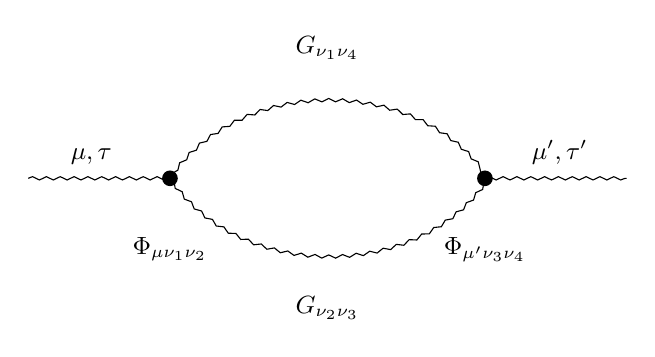
\begin{tikzpicture}[every node/.style={font=\small}]
  \coordinate (v1) at (0,0);  \coordinate (v2) at (4,0);
  \draw[phonon] (-1.8,0) -- (v1);
  \draw[phonon] (v2)      -- (5.8,0);
  \node[above] at (-1.0, 0.05) {$\mu,\tau$};
  \node[above] at ( 4.95,0.05) {$\mu',\tau'$};
  \draw[phonon] (v1) to[bend left=55]  (v2);
  \draw[phonon] (v1) to[bend right=55] (v2);
  \node at (2, 1.65) {$G_{\nu_1\nu_4}$};
  \node at (2,-1.65) {$G_{\nu_2\nu_3}$};
  \node[fc3 vertex] at (v1) {};
  \node[fc3 vertex] at (v2) {};
  \node[below=18pt] at (v1) {$\Phi_{\mu\nu_1\nu_2}$};
  \node[below=18pt] at (v2) {$\Phi_{\mu'\nu_3\nu_4}$};
\end{tikzpicture}
\caption{Sunset (two-vertex bubble) Feynman diagram for the leading
$(\Phi^{(3)})^2$ phonon--phonon self-energy of
\cref{eq:sigma_sunset_contour}. Wavy lines denote phonon propagators
$G$, filled circles denote cubic FC3 vertices. The two equivalent
internal lines produce the symmetry factor $\tfrac{1}{2}$.}
\label{fig:sunset_diagram}
\end{figure}


To order $(\Phi^{(3)})^2$, the proper self-energy is given by the
``sunset'' diagram (\cref{fig:sunset_diagram}), in which two cubic
vertices are connected by two internal phonon propagators. The
value of the diagram, including all combinatorial factors,
is~\cite{guo_quantum_2020,wang_nonequilibrium_2014}
\begin{equation}\label{eq:sigma_sunset_contour}
  \Sigma^{(2)}_{\mu\mu'}(\tau,\tau')
  = \frac{i\hbar}{2}\sum_{\nu_1\nu_2\nu_3\nu_4}
    \Phi_{\mu\nu_1\nu_2}\,
    G_{\nu_1\nu_4}(\tau,\tau')\,
    G_{\nu_2\nu_3}(\tau,\tau')\,
    \Phi_{\mu'\nu_3\nu_4}.
\end{equation}

\begin{figure}[ht]
\centering
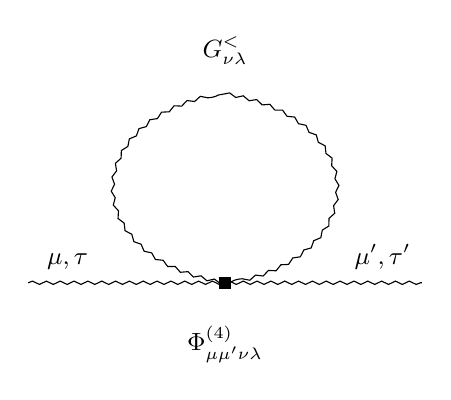
\begin{tikzpicture}[every node/.style={font=\small}]
  \coordinate (v) at (0,0);
  \draw[phonon] (-2.5,0) -- (v);
  \draw[phonon] (v)      -- (2.5,0);
  \node[above] at (-2.0, 0.05) {$\mu,\tau$};
  \node[above] at ( 2.0, 0.05) {$\mu',\tau'$};
  \draw[phonon] (v) to[bend left=80, looseness=2.0] (0,2.4);
  \draw[phonon] (0,2.4) to[bend left=80, looseness=2.0] (v);
  \node at (0,2.95) {$G^{<}_{\nu\lambda}$};
  \node[fc4 vertex] at (v) {};
  \node[below=12pt] at (v) {$\Phi^{(4)}_{\mu\mu'\nu\lambda}$};
\end{tikzpicture}
\caption{Hartree--Fock (one-loop) tadpole self-energy from a single
quartic FC4 vertex. The filled square denotes
$\Phi^{(4)}_{\mu\mu'\nu\lambda}$. The two internal lines contract into
the closed loop $G^{<}_{\nu\lambda}(\tau,\tau)$. The diagram is real
and frequency-independent and acts as a temperature-dependent
renormalisation $D\mapsto D + \Sigma^{(4),\mathrm{HF}}$.}
\label{fig:fc4_tadpole}
\end{figure}


A second diagram, lower order in derivatives but one loop, survives:
the FC4 Hartree--Fock ``loop'' tadpole
$\Sigma^{(4),\mathrm{HF}}_{\mu\mu'} = -\tfrac{\hbar}{2}
\sum_{\nu\lambda} \Phi^{(4)}_{\mu\mu'\nu\lambda}\,
G^{<}_{\nu\lambda}(\tau,\tau)$ from a single quartic vertex (\cref{fig:fc4_tadpole}).
The loop self-energy is real and frequency-independent.
It therefore produces no phonon linewidth, but shifts the phonon
dispersion, $D \mapsto D + \Sigma^{(4),\mathrm{HF}}$, providing the
leading temperature-dependent mode renormalisation of self-consistent
phonon theory~\cite{tadano_first-principles_2018,wang_nonequilibrium_2014}. In a
transport-focused SCBA targeting the imaginary part of $\Sigma_s$, the
loop can be absorbed into a renormalised harmonic spectrum
computed independently (e.g.\ via SCP or
SSCHA~\cite{paulatto_first-principles_2015,tadano_first-principles_2018}) and is not
re-included diagram-by-diagram in the iteration.

The factor $1/2$ above corresponds to the fully-symmetric FC3
$\Phi_{\mu\nu\lambda}$ defined by
$\Phi_{\mu\nu\lambda} = \partial^3 V/(\partial u_\mu \partial u_\nu \partial u_\lambda)$,
divided by $3!$ in \cref{eq:H_phonon}. ~\citet{mingo_anharmonic_2006} obtains an extra factor of $\pi/9$
which~\citet{guo_quantum_2020} attribute to a different convention in
the symmetrization of the cubic vertex.

Applying the Langreth analytic continuation rules~\cite{devreese_linear_1976,haug_quantum_2008}
to the contour product of two $G$'s in
\cref{eq:sigma_sunset_contour} yields real-time lesser/greater
components,
\begin{equation}\label{eq:sigma_guo}
  \Sigma^{\gtrless}_{\mu\mu'}(\omega)
  = \frac{i\hbar}{2}
    \sum_{\nu_1\nu_2\nu_3\nu_4}
    \Phi_{\mu\nu_1\nu_2}
    \left[
      \int\frac{d\omega'}{2\pi}\,
      G^{\gtrless}_{\nu_1\nu_4}(\omega')\,
      G^{\gtrless}_{\nu_2\nu_3}(\omega-\omega')
    \right]
    \Phi_{\mu'\nu_3\nu_4},
\end{equation}
which is the form derived in detail in~\cite{wang_nonequilibrium_2014,guo_quantum_2020}.
The convolution enforces the
energy-conservation $\delta(\omega - \omega' - \omega'')$ implicit in
the contour integral. Substituting equilibrium FDT
\cref{eq:phonon_fdt} reproduces Fermi's-golden-rule expressions for
three-phonon scattering rates: in mode basis,
\begin{align}\label{eq:fgr}
  \mathrm{Im}\,\Sigma^R_s(\omega_s,\qp)
  &\;=\;
   -\,\frac{\pi\hbar}{8 \omega_s(\qp)}
   \sum_{s_1 s_2}\sum_{\qp{}'}
   |V_3(s\qp; s_1\qp{}'; s_2,\qp{-}\qp{}')|^2 \notag\\
  &\quad\times
   \Bigl\{
     [1 + n_1 + n_2]\,\delta(\omega_s - \omega_{s_1} - \omega_{s_2})
     + 2[n_1 - n_2]\,\delta(\omega_s - \omega_{s_1} + \omega_{s_2})
   \Bigr\},
\end{align}
with $n_i = n_{\mathrm{BE}}(\omega_{s_i},T)$, exhibiting the
splitting/recombination ($1\to 2$) channel and the absorption ($2\to 1$)
channel. This expression coincides with the Boltzmann result of~\citet{klemens_anharmonic_1966}
in the relaxation-time approximation,.

\subsubsection{Retarded self-energy}
\label{subsub:KK}

By construction $\Sigma^R$ is causal in time, so its frequency
components satisfy a Kramers--Kronig relation. Starting from
$\Sigma^R = \tfrac{1}{2}(\Sigma^t + \Sigma^{\bar{t}}) +
\tfrac{1}{2}(\Sigma^> - \Sigma^<)$ and using the spectral identity for
$\Sigma^{t,\bar{t}}$, one obtains~\cite{guo_quantum_2020,wang_nonequilibrium_2014}
\begin{equation}\label{eq:sigma_R_full}
  \Sigma^R(\omega)
  = \tfrac{1}{2}\bigl[\Sigma^>(\omega) - \Sigma^<(\omega)\bigr]
    + i\,\mathcal{P}\!\!\int_{-\infty}^{\infty}\!\frac{d\omega'}{2\pi}\,
      \frac{\Sigma^>(\omega') - \Sigma^<(\omega')}{\omega - \omega'}.
\end{equation}
The antihermitian (dissipative) first term carries inverse-lifetime
information,
\begin{equation}\label{eq:lifetime}
  \tau_s^{-1}(\qp)
  \equiv -\frac{2}{\hbar\omega_s(\qp)}\,
     \mathrm{Im}\,\langle s|\Sigma^R(\omega_s,\qp)|s\rangle,
\end{equation}
while the dispersive second term encodes the anharmonic frequency
renormalization $\Delta\omega_s \approx
\mathrm{Re}\,\Sigma^R/(2\omega_s)$ (mode hardening or softening).
Numerical evaluation of the principal value is expensive, so in practice
the dispersive part is often dropped:
\begin{equation}\label{eq:sigma_r}
  \Sigma^R(\omega)
  \approx \tfrac{1}{2}\bigl[\Sigma^>(\omega) - \Sigma^<(\omega)\bigr].
\end{equation}

\subsubsection{Detailed balance}

The $\Sigma^{\gtrless}$ of \cref{eq:sigma_guo} satisfy detailed balance
at equilibrium,
\begin{equation}\label{eq:detailed_balance}
  \Sigma^>(\omega) = e^{\beta\hbar\omega}\,\Sigma^<(\omega),
\end{equation}
which together with the Keldysh equation \cref{eq:keldysh_eq}
guarantees that $G^{\lessgtr}$ also satisfy detailed balance, recovering
\cref{eq:phonon_fdt} when $\Sigma_L,\Sigma_R$ correspond to a single
temperature. The presence of two leads at different temperatures breaks
detailed balance and drives a steady-state heat current.

\subsubsection{Higher-order corrections}
\label{subsub:higher_order}
\begin{figure}[ht]
\centering
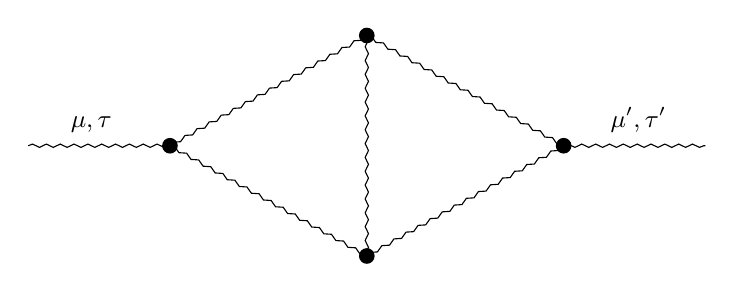
\begin{tikzpicture}[every node/.style={font=\small}]
  \coordinate (v1) at (0,0);     \coordinate (v2) at (5,0);
  \coordinate (vt) at (2.5, 1.4);  \coordinate (vb) at (2.5,-1.4);
  \draw[phonon] (-1.8,0) -- (v1);
  \draw[phonon] (v2)      -- (6.8,0);
  \node[above] at (-1.0, 0.05) {$\mu,\tau$};
  \node[above] at ( 5.95,0.05) {$\mu',\tau'$};
  \draw[phonon] (v1) -- (vt);   \draw[phonon] (v1) -- (vb);
  \draw[phonon] (vt) -- (v2);   \draw[phonon] (vb) -- (v2);
  \draw[phonon] (vt) -- (vb);
  \foreach \pt in {v1,v2,vt,vb}{\node[fc3 vertex] at (\pt) {};}
\end{tikzpicture}
\caption{Two-loop $\Phi^{(3)}$ vertex correction to the phonon
self-energy ($\mathcal{O}((\Phi^{(3)})^4)$). Four cubic vertices form a
1PI ``diamond'' subgraph}
\label{fig:vertex_correction}
\end{figure}

\begin{figure}[ht]
\centering
\begin{subfigure}[b]{0.95\linewidth}
\centering
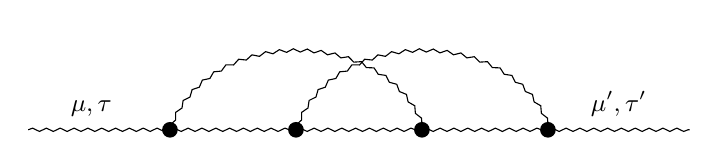
\begin{tikzpicture}[every node/.style={font=\small}]
  \coordinate (v1) at (0  ,0);  \coordinate (v2) at (1.6,0);
  \coordinate (v3) at (3.2,0);  \coordinate (v4) at (4.8,0);
  \draw[phonon] (-1.8,0) -- (v1);
  \draw[phonon] (v4)      -- (6.6,0);
  \node[above] at (-1.0,0.05) {$\mu,\tau$};
  \node[above] at ( 5.7,0.05) {$\mu',\tau'$};
  \draw[phonon] (v1) -- (v2);
  \draw[phonon] (v2) -- (v3);
  \draw[phonon] (v3) -- (v4);
  \draw[phonon] (v1) to[bend left=70, looseness=1.1] (v3);
  \draw[phonon] (v2) to[bend left=70, looseness=1.1] (v4);
  \foreach \pt in {v1,v2,v3,v4}{\node[fc3 vertex] at (\pt) {};}
\end{tikzpicture}
\caption{Crossed two-loop self-energy graph at order
$(\Phi^{(3)})^4$.}
\label{fig:crossed_graph}
\end{subfigure}

\vspace{1em}
\begin{subfigure}[b]{0.95\linewidth}
\centering
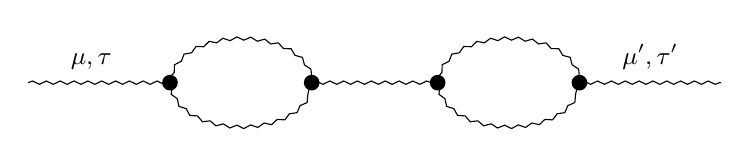
\begin{tikzpicture}[every node/.style={font=\small}]
  \coordinate (v1) at (0  ,0);   \coordinate (v2) at (1.8,0);
  \coordinate (v3) at (3.4,0);   \coordinate (v4) at (5.2,0);
  \draw[phonon] (-1.8,0) -- (v1);
  \draw[phonon] (v4)      -- (7.0,0);
  \node[above] at (-1.0,0.05) {$\mu,\tau$};
  \node[above] at ( 6.1,0.05) {$\mu',\tau'$};
  \draw[phonon] (v1) to[bend left=80]  (v2);
  \draw[phonon] (v1) to[bend right=80] (v2);
  \draw[phonon] (v3) to[bend left=80]  (v4);
  \draw[phonon] (v3) to[bend right=80] (v4);
  \draw[phonon] (v2) -- (v3);
  \foreach \pt in {v1,v2,v3,v4}{\node[fc3 vertex] at (\pt) {};}
\end{tikzpicture}
\caption{Ladder topology at order $(\Phi^{(3)})^4$:
two sunset bubbles connected by a single line.}
\label{fig:ladder_graph}
\end{subfigure}

\caption{Non-trivial two-loop self-energy topologies at order
$(\Phi^{(3)})^4$ that lie beyond bubble-SCBA.}
\label{fig:two_loop_topologies}
\end{figure}

\Cref{eq:sigma_guo} captures the leading three-phonon process. Higher
orders include~\cite{wang_nonequilibrium_2014,guo_quantum_2020}:
(i) the four-phonon tadpole from $\Phi^{(4)}$,
$\Sigma^{(4),\mathrm{HF}}_{\mu\mu'} = -\tfrac{\hbar}{2}\sum_{\nu\lambda}
\Phi^{(4)}_{\mu\mu'\nu\lambda}\,G^<_{\nu\lambda}(\tau,\tau)$,
which is real, frequency-independent, and renormalizes
$D \mapsto D + \Sigma^{(4),\mathrm{HF}}$, contributing the
temperature-dependent thermal expansion and frequency
shifts~\cite{wang_nonequilibrium_2014} (\cref{fig:fc4_tadpole}),
(ii) the two-loop $\Phi^{(3)}$ vertex correction, relevant at high
$T$ where $\hbar\omega_{\max}/k_B T \lesssim 1$ and three-phonon
processes saturate (\cref{fig:vertex_correction}) and
(iii) crossed and ladder graphs that are needed to maintain
$\Phi$-derivability.

The $\Phi$-derivability framework of Baym and Kadanoff~\cite{baym_conservation_1961, baym_self-consistent_1962}
states that $\Sigma$ must be the functional derivative of a generating
functional $\Phi[G]$ for the conservation laws (energy, particle number)
to be satisfied identically. The sunset diagram of
\cref{eq:sigma_sunset_contour} is $\Phi$-derivable when the same
$G$ enters both internal lines, but only asymptotically as the
SCBA iteration converges~\cite{lee_anharmonic_2018}. This is e.g. addressed by
the LOA-based scheme of~\citet{lee_anharmonic_2018}
which is exactly conserving at every iteration.

\subsubsection{Transverse periodic case}

For a 3D system with periodicity transverse to transport, the
self-energy acquires a $\qp$ argument and an internal sum over
transverse momenta~\cite{guo_quantum_2020}:
\begin{align}\label{eq:sigma_phph}
  \sse{\gtrless}_{x x'}(\omega,\qp)
  = \frac{i\hbar}{2}
    &\sum_{y_1 y_2 y_3 y_4}
    \frac{1}{N}\sum_{\qp{}'}
    \tilde{\Phi}_{x y_1 y_2}\!\bigl(\qp{}',\qp - \qp{}'\bigr)\,
    \tilde{\Phi}_{x' y_3 y_4}\!\bigl(\qp{}'-\qp,-\qp{}'\bigr)
    \notag\\
  &\times
    \int\!\dw\;
    G^{\gtrless}_{y_1 y_4}(\omega',\qp{}')\,
    G^{\gtrless}_{y_2 y_3}(\omega-\omega',\qp - \qp{}'),
\end{align}
where $x,y$ denote transport-direction DOF indices, i.e.\ $x=(l_x,\mu)=(l_x,\kappa,\alpha)$
with $l_x$ enumerating transport-direction slabs/supercells. The
partially Fourier-transformed FC3 entering this expression is
\begin{align}\label{eq:fc3_fourier}
  \tilde{\Phi}_{x y_1 y_2}(\qp,\qp{}')
  = \tilde{\Phi}^{l m_1 m_2}_{\mu \nu_1 \nu_2}(\qp,\qp{}')
  = \sum_{\substack{n_1,\,n_2\\ n_{ix}=m_{ix}}}
    \Phi^{l n_1 n_2}_{\mu \nu_1 \nu_2}\;
    e^{-i\qp\cdot (n_1 - m_1)}\;
    e^{-i\qp{}'\cdot (n_2 - m_2)},
\end{align}
i.e.\ the sum runs over transverse supercells at fixed transport-direction
cell. Unlike the harmonic FC2 object which depends on a single
transverse wavevector, the cubic tensor depends on two: the
$\qp{}'$ sum couples all transverse wavevectors, so evaluating
$\Sigma_s(\qp)$ requires Green's functions at every $\qp{}'$, destroying
the embarrassing parallelism of the ballistic problem. The arithmetic
complexity scales as $\mathcal{O}(N_q^2 N_\omega^2 N_{\mathrm{DOF}}^4)$
before any low-rank or stochastic acceleration. This is the dominant
cost of the anharmonic simulation, as reported in~\cite{luisier_atomistic_2012,guo_quantum_2020, lee_anharmonic_2018}.

% ----------------------------------------------------------------------
\subsection{Observables}
\label{sub:negf_obs}
% ----------------------------------------------------------------------

We collect the observables computable from $G^{R,A,\lessgtr}$ in both
the ballistic and anharmonic regimes.

\subsubsection{Spectral function and local density of states}

The spectral function and LDOS are
\begin{equation}\label{eq:dos}
  A(\omega^2) = i[G^R - G^A],
  \qquad
  \rho_\mu(\omega^2) = \frac{1}{\pi}\,A_{\mu\mu}(\omega^2),
\end{equation}
related to the standard $\omega$-resolved density of states by
$\rho(\omega) = 2\omega\,\rho(\omega^2)$. In the transverse periodic
case $\rho_\mu(\omega) = (2\omega/N_q)\sum_{\qp} A_{\mu\mu}(\omega^2,\qp)/\pi$.

\subsubsection{Ballistic transmission and conductance}

In the ballistic limit ($\Sigma_s = 0$) the transmission function is
given by the Caroli formula~\cite{caroli_direct_1971,mingo_calculation_2003,wang_nonequilibrium_2007},
\begin{equation}\label{eq:caroli}
  \mathcal{T}(\omega^2,\qp)
  = \mathrm{Tr}\bigl[\Gamma_L\,G^R\,\Gamma_R\,G^A\bigr],
\end{equation}
with the transverse-averaged transmission
\begin{equation}
  \bar{\mathcal{T}}(\omega^2)
  = \frac{1}{N_q}\sum_{\qp} \mathcal{T}(\omega^2,\qp).
\end{equation}
The thermal conductance per unit area is the Landauer integral
\begin{equation}\label{eq:G_thermal}
  G(T)
  = \frac{1}{A_c}\int_0^\infty\!\frac{d\omega}{2\pi}\;
    \bar{\mathcal{T}}(\omega)\,\hbar\omega\,
    \frac{\partial n_\mathrm{BE}}{\partial T},
\end{equation}
with $A_c$ the cross-sectional area and
\begin{equation}
  \frac{\partial n_\mathrm{BE}}{\partial T}
  = \frac{\hbar\omega}{k_B T^2}\,
    \frac{e^{\hbar\omega/k_B T}}
         {(e^{\hbar\omega/k_B T}-1)^2}.
\end{equation}
The integrand vanishes at both endpoints, so a trapezoidal rule on the
sampled frequency grid suffices.

\subsubsection{Mode-resolved transmission}

Diagonalizing $\Gamma_\ell$ at fixed $(\omega,\qp)$ yields incoming and
outgoing mode bases of the leads. Writing $\Gamma_L = U_L \Lambda_L
U_L^\dagger$ and similarly for $R$, the transmission matrix element from
incoming mode $m\in L$ to outgoing mode $m'\in R$ is
\begin{equation}\label{eq:mode_T}
  t_{m'm}(\omega,\qp)
  = \sqrt{\Lambda_R^{m'}}\,
    \bigl[U_R^\dagger G^R U_L\bigr]_{m'm}\,
    \sqrt{\Lambda_L^{m}},
\end{equation}
with $\sum_{m'm}|t_{m'm}|^2 = \mathcal{T}$. This is the phonon analogue
of the Fisher--Lee relation~\cite{fisher_relation_1981}.
For phonons the mode-matching formulation~\cite{ong_efficient_2015}
provides an alternative route to the same
quantity through the eigenproblem of the bulk transfer matrix.

\subsubsection{Meir--Wingreen heat current}

In the anharmonic regime the Caroli formula no longer holds: there is
no $\mathcal{T}(\omega)$ that captures both elastic and inelastic
processes. The generalization is the phonon Meir--Wingreen
formula~\cite{meir_landauer_1992,wang_nonequilibrium_2007,wang_quantum_2008},
\begin{equation}\label{eq:meir_wingreen}
  I_L
  = \int_0^\infty\!\frac{d\omega}{4\pi}\,\hbar\omega\,
    \mathrm{Tr}\bigl[
      \Sigma_L^<(\omega)\,G^>(\omega)
    - \Sigma_L^>(\omega)\,G^<(\omega)
    \bigr].
\end{equation}
\Cref{eq:meir_wingreen} is exact for any
many-body $\Sigma_s$, provided $G^{\lessgtr}$ are obtained from the full
Keldysh equation \cref{eq:keldysh_eq}. In the ballistic limit, the
Keldysh equation gives $G^{<} = G^R(\Sigma_L^< + \Sigma_R^<)G^A$, and
substitution into \cref{eq:meir_wingreen} reproduces \cref{eq:caroli}
weighted by $\hbar\omega[n_L-n_R]$, recovering Landauer.

\subsubsection{Local heat current and conservation}

The bond-resolved heat current of Hardy~\cite{hardy_energy-flux_1963} can provide atomic insight.
Between two transport-direction slabs $i$
and $j = i + 1$,
\begin{equation}\label{eq:I_local}
  I_{i,i+1}
  = -\int_0^\infty\!\frac{d\omega}{2\pi}\,\hbar\omega\,
    \mathrm{Re}\,\mathrm{Tr}\bigl[H_{i,i+1}\,G^<_{i+1,i}(\omega)\bigr],
\end{equation}
with $H_{i,i+1}$ the inter-slab coupling block. In a converged SCBA
solution the steady-state continuity equation enforces $I_{i,i+1}$
independent of $i$ throughout the device, providing physically meaningful convergence test:
\begin{equation}
  \delta I = \max_i I_{i,i+1} - \min_i I_{i,i+1}
\end{equation}
measures the violation of energy conservation by approximations in
$\Sigma_s$ (incomplete SCBA iteration, Hilbert-transform truncation,
finite frequency grid). A convergence criteron for SCBA can be
$\delta I/\bar I \lesssim \varepsilon$~\cite{luisier_atomistic_2012,guo_quantum_2020} for
appropriate $\varepsilon$ (e.g. $10^{-3}$ in \cite{guo_quantum_2020}).

Heat conservation at the level of \cref{eq:sigma_sunset_contour}
is guaranteed by $\Phi$-derivability~\cite{baym_self-consistent_1962} only at full
self-consistency. At any finite iteration count, $\delta I/\bar I$ is
non-zero. The Hilbert-transform neglect of \cref{eq:sigma_r} introduces an additional
$\mathcal{O}(\Delta\omega/\omega)$ conservation error.

% ----------------------------------------------------------------------
\subsection{SCBA iterations}
\label{sub:scba}
% ----------------------------------------------------------------------

\Cref{eq:system,eq:keldysh_eq,eq:sigma_phph,eq:sigma_r} together define
a nonlinear fixed-point problem $\Sigma_s = \mathcal{F}[G[\Sigma_s]]$,
solved iteratively in the SCBA. Convergence is two-fold: numerical
(consecutive iterates close in some norm) and physical (current
conservation, \cref{eq:I_local}). Mixing schemes are necessary because
pure fixed-point iteration of \cref{eq:sigma_phph} is often divergent or
oscillatory at finite anharmonicity~\cite{wang_nonequilibrium_2007,luisier_atomistic_2012}.

\subsubsection{Linear mixing}

The simplest scheme,
\begin{equation}\label{eq:linear_mix}
  \Sigma^{(n+1)} = (1-\alpha)\,\Sigma^{(n)} + \alpha\,\Sigma^{\mathrm{new}},
\end{equation}
with damping parameter $\alpha \in (0,1]$. Linear mixing converges if
the fixed-point Jacobian
$J = \partial\mathcal{F}/\partial\Sigma_s$ has spectral radius
$\sigma(I - \alpha J) < 1$, i.e.\ $\alpha < 2/(1+|\sigma(J)|_{\max})$.
For weak anharmonicity ($|\sigma(J)|<1$) any $\alpha \le 1$ works; for
strong anharmonicity the spectrum of $J$ extends close to $-1$ in
some directions and small $\alpha\sim 0.1\text{--}0.3$ is required, with
linear convergence rate $1-\alpha$ in the slowest mode.

\subsubsection{Anderson mixing}

Anderson acceleration~\cite{anderson_iterative_1965} constructs a quasi-Newton
update from a history of residuals,
\begin{equation}\label{eq:anderson}
  \vc{x}_{k+1}
  = \bigl(\vc{x}_k + \alpha\,\vc{f}_k\bigr)
    - \bigl(\Delta\vc{X} + \alpha\,\Delta\vc{F}\bigr)\,\vc{\gamma}_k,
\end{equation}
with $\vc{f}_k = G(\vc{x}_k) - \vc{x}_k$ the residual,
$\Delta\vc{X}, \Delta\vc{F}$ the matrices of consecutive iterate and
residual differences, and $\vc{\gamma}_k$ solving the regularized
least-squares problem
\begin{equation}
  (\Delta\vc{F}^H \Delta\vc{F} + \lambda \mathbb{I})\,\vc{\gamma}
  = \Delta\vc{F}^H \vc{f}_k,
  \qquad
  \lambda = 10^{-8}\,\tr(\Delta\vc{F}^H \Delta\vc{F}).
\end{equation}
For linear problems Anderson mixing is
essentially equivalent to GMRES applied to the residual
equation~\cite{walker_anderson_2011,rohwedder_analysis_2011}, with provable
$q$-linear convergence with $q$-factor $q = 3c - c^2$ for depth-1
Anderson when the underlying iteration is a contraction with constant
$c < 2-\sqrt{3}$~\cite{toth_convergence_2015,bian_anderson_2021}. Local
convergence in nonlinear electronic-structure problems is well
established under mild Lipschitz assumptions on the
fixed-point map~\cite{rohwedder_analysis_2011,toth_convergence_2015}. In
practice, Anderson mixing dramatically accelerates convergence when the
fixed-point equation is well-conditioned, with rates approaching that
of Newton's method. However, storing the history is often prohibitive, so that
Anderson mixing becomes infeasible for large structures.

\subsubsection{Convergence diagnostics}

We monitor three quantities across iterations: (i) the relative
Frobenius norm
$\|\Sigma_s^{(n+1)}-\Sigma_s^{(n)}\|/\|\Sigma_s^{(n)}\|$,
(ii) the conductance $G(T)$ from \cref{eq:G_thermal} or, in the
inelastic case, the Meir--Wingreen current, and (iii) the slab-resolved
current imbalance $\delta I/\bar I$. Convergence is declared when (i)
and (iii) fall below prescribed tolerances simultaneously.

\subsubsection{Lowest-order approximation.}

An attractive alternative to direct SCBA, developed by~\citet{lee_anharmonic_2018,lee_quantum_2019}, is the
lowest-order approximation (LOA) implemented through Padé
resummation. LOA collects only the conserving ($\Phi$-derivable) diagrams
at each order in $\Phi^{(3)}$, ensuring exact current conservation
at every iteration, then accelerates the resulting series by
Padé approximants. Compared to SCBA, LOA achieves comparable accuracy
at $\sim 2\times$ lower cost for thermal transport in 3D
nanostructures~\cite{lee_anharmonic_2018}.

% ----------------------------------------------------------------------
\subsection{Decay properties and Truncation errors}
\label{sub:decay}
% ----------------------------------------------------------------------

Truncations at every step (real-space FC cutoff, finite device length, finite $\omega$ grid,
finite Sancho-Rubio iteration count) introduce errors with
quantifiable scaling. We summarize, from first principles, the decay
rates of each of the involved quantities.

\subsubsection{Real-space decay of harmonic force constants}
\label{subsub:fc2_decay}

The asymptotic behaviour of $\Phi^{(2)}(R)$ at large $|R|$ is controlled
by the analytic structure of the dielectric response of the underlying
electronic system. \Citet{cances_decay_2025} prove the following
within the reduced Hartree--Fock (or random-phase
approximation) model:

\paragraph{Insulators at zero electronic temperature.}
The dynamical matrix $D(\qp)$ is singular at $\qp = 0$, with the
non-analytic dipole--dipole structure given in~\cite{cochran_dielectric_1962}:
\begin{equation}\label{eq:fc2_dipole}
  D^{\mathrm{LR}}_{\kappa\alpha,\kappa'\beta}(\qp \to 0)
  \;\sim\;
  \frac{4\pi}{\Omega_{\mathrm{cell}}}\,
  \frac{(\qp\cdot Z^*_{\kappa})_\alpha\,(\qp\cdot Z^*_{\kappa'})_\beta}
       {\qp\cdot \epsilon_\infty\cdot \qp},
\end{equation}
where $Z^*_\kappa$ is the Born effective charge tensor of atom $\kappa$
and $\epsilon_\infty$ the optical dielectric tensor. Inverse Fourier
transform of this $\qp\to 0$ singularity gives an algebraic
real-space tail to $\Phi$.

\paragraph{Materials at finite electronic temperature (metals).}
\Citet{cances_decay_2025} prove that the
dynamical matrix is analytic in $\qp$, and
$\Phi^{(2)}(R)$ decays exponentially:
\begin{equation}\label{eq:fc2_metal}
  |\Phi^{(2)}(R)|\;\le\;C\,e^{-|R|/\xi_e},\qquad
  \xi_e \;\sim\;\frac{\hbar v_F}{k_B T_{\mathrm{el}}}.
\end{equation}

\paragraph{Concrete truncation error.}
Truncating at distance $R_c$ introduces an error in the dynamical matrix
of order
\begin{equation}\label{eq:fc2_error_metal}
  \|D(\qp) - D^{R_c}(\qp)\| \;\lesssim\;C \frac{e^{-R_c/\xi_e}}{1 - e^{-1/\xi_e}}
  \quad\text{(metals, exponential)},
\end{equation}
or, in polar insulators, $\sim 1/R_c^3$ for the bare truncation, but
$\sim e^{-R_c/\xi_e}$ if the short-range part once the
$1/r^3$ Cochran--Cowley tail has been subtracted analytically and added
back exactly via Ewald summation~\cite{gonze_dynamical_1997}.

\subsubsection{Transverse $\qp$-mesh convergence}
\label{subsub:qp_decay}

The convergence of observables in $N_q$ depends on the differentiability
of the integrand. For the Caroli formula \cref{eq:caroli}, the
$\qp$-integrand is generically smooth and trapezoidal Monkhorst--Pack
sampling converges as $\mathcal{O}(N_q^{-2})$ in 2D. At Brillouin-zone boundaries or near van
Hove singularities, convergence degrades to $\mathcal{O}(N_q^{-1})$;
a Gaussian smearing or tetrahedron method may then be preferable. The
self-energy convolution \cref{eq:sigma_phph} couples $\qp$ and $\qp{}'$,
so the effective integrand has $N_q^{-1/2}$ statistical-noise structure
under random sampling, but adaptive importance sampling can recover
$\mathcal{O}(N_q^{-1})$ ~\cite{lee_anharmonic_2018}.

\subsubsection{Convergence rate of Sancho-Rubio decimation revisited}

As discussed in \cref{sub:contact_se}, the decimation iteration
\cref{eq:sr_eps_s,eq:sr_eps,eq:sr_alpha,eq:sr_beta} effectively doubles
the number of decimated layers at each step, with iterates obeying
$\|\alpha_n\|, \|\beta_n\| \sim \rho^{2^n}$ inside gaps and
$e^{-c\eta\cdot 2^n}$ on bands. The practical implication is that
\emph{doubling the tolerance roughly costs one extra iteration}; total
cost is $\mathcal{O}(N_\omega\,N_q\,N_{\mathrm{DOF}}^3\,N_{\mathrm{iter}})$
with $N_{\mathrm{iter}}$ essentially constant (and small,
$\sim 10\text{--}30$).

% ----------------------------------------------------------------------
\section{Computation of the Phonon-Phonon Scattering Self Energy}
\label{sec:phph_computation}
% ----------------------------------------------------------------------

The phonon-phonon SSE in \cref{eq:sigma_phph} involves three computational
steps that dominate the cost of an SCBA iteration of the anharmonic
SCAB equations: a four-index ring
contraction over $y_1,y_2,y_3,y_4$, an internal sum over the
transverse wavevector $\qp'$, and a frequency convolution along
$\omega$. The frequency convolution is structurally identical to the
polarisation that appears in the GW formalism
\cite{deuschle_electron-electron_2025},
\begin{equation}\label{eq:gw_polarization}
  P_{ij}^{\gtrless}(E)
  = -i \int dE'\;
       G_{ij}^{\gtrless}(E')\,G_{ji}^{\gtrless}(E'-E),
\end{equation}
and reuses the same FFT-based machinery. The $\qp'$-sum couples
distinct transverse wavevectors through the FC3 vertices
$\tilde\Phi$ and is unique to the transverse-periodic geometry. The
inner four-index contraction has no analogue in GW: in
\cref{eq:gw_polarization}, the contraction structure of $P$ is local
in the orbital pair $(i,j)$, whereas the phonon bubble couples
$y_1,\dots,y_4$ across the supercell. In what follows we omit the
$\gtrless$ superscripts unless the distinction matters; all
derivations apply unchanged to lesser, greater, and (via the
fluctuation--dissipation construction of \cref{eq:sigma_r}) retarded
self-energies.

% ----------------------------------------------------------------------
\subsection{Frequency convolution and discretisation}
\label{ssec:phph_freq}
% ----------------------------------------------------------------------

The integrand in \cref{eq:sigma_phph} contains a single frequency
convolution $\int d\omega'\;G_1(\omega')\,G_2(\omega-\omega')$. We
turn it into a pointwise product in time through the Fourier
transform pair
\begin{equation}\label{eq:g_tau}
  g(\tau;\cdot)
  = \int\!\frac{d\omega}{2\pi}\;
    G(\omega;\cdot)\,e^{-i\omega\tau},
  \qquad
  G(\omega;\cdot)
  = \int\!d\tau\;g(\tau;\cdot)\,e^{+i\omega\tau},
\end{equation}
under which the 1D convolution theorem gives
\begin{equation}\label{eq:omega_conv}
  \int\!d\omega'\;
    G_1(\omega';\cdot)\,G_2(\omega-\omega';\cdot)
  = \int\!d\tau\;
    g_1(\tau;\cdot)\,g_2(\tau;\cdot)\,e^{+i\omega\tau}.
\end{equation}
Substituting \cref{eq:omega_conv} into \cref{eq:sigma_phph}, the
bubble takes the $\tau$-domain form
\begin{equation}\label{eq:sigma_phph_tau}
\begin{aligned}
  \Sigma_{xx'}(\omega;\qp)
  = \frac{i\hbar}{2}
    &\sum_{y_1y_2y_3y_4}
    \frac{1}{N}\sum_{\qp'}
    \tilde\Phi_{xy_1y_2}(\qp',\qp-\qp')\,
    \tilde\Phi_{x'y_3y_4}(\qp'-\qp,-\qp')\\
    &\times\int\!d\tau\;
    g_{y_1y_4}(\tau;\qp')\,g_{y_2y_3}(\tau;\qp-\qp')\,
    e^{+i\omega\tau}.
\end{aligned}
\end{equation}
The $\omega$-integral has been replaced by a $\tau$-integral, the
two propagators are now multiplied pointwise, and a
final $\tau\to\omega$ Fourier transform delivers
$\Sigma$ on the original frequency grid.

\paragraph{Discrete frequency grid.} Numerically, the SSE is
evaluated on a uniform grid
$\omega_n = \omega_\mathrm{min} + n\Delta\omega$ for
$n=0,\ldots,N_\omega-1$, with broadening
$\eta = \eta_\mathrm{factor}(\Delta\omega)^{2}$ to suppress
spurious poles at the resolution scale of the grid. The convolution
is evaluated by FFT on a zero-padded grid of length
\begin{equation}\label{eq:nfft_pad}
  N_\mathrm{fft} = 2N_\omega - 1,
\end{equation}
which is the smallest length that avoids cyclic wrap-around between
the two factors when both have support of width $N_\omega$. Stages~1 and~3
(\cref{ssec:phph_distribution}) operate on $N_\mathrm{fft}$-long
arrays, the SSE on the original grid is recovered by truncation to
the first $N_\omega$ points after the inverse FFT.

\paragraph{Convolution support: $f_{\max}\!\ge\!2\omega_{\max}/2\pi$.}
The harmonic Green's functions $G^{\gtrless}(\omega)$ have spectral
support bounded by the largest phonon frequency $\omega_{\max}$ of the
device, i.e.\ the spectrum of
$H_{00}+H_{01}+H_{01}^{\dagger}$. The product
$g_1(\tau)\,g_2(\tau)$ in \cref{eq:omega_conv} has Fourier support
that is the convolution sum of the individual supports, so
$\Sigma^{\gtrless}(\omega)$ is nonzero on
\begin{equation}\label{eq:conv_support}
  \omega\in[-2\omega_{\max},\,2\omega_{\max}]
\end{equation}
and only there. The truncated linear convolution \cref{eq:nfft_pad} is
unbiased on that interval \emph{only when the grid covers it}, i.e.\
when $f_{\max}\ge 2\omega_{\max}/2\pi$. If the grid is shorter,
$f_{\max}<2\omega_{\max}/2\pi$, the bubble contributions at
$|\omega|\in(f_{\max},2\omega_{\max})$ are missing from the inverse
FFT and, on a discrete grid, the residual aliases back into the
visible window. The bubble then carries large spurious contributions
that fake a strong-coupling self-energy and drive the SCBA loop
unstable. The required grid size is therefore set by the stiffest
mode of the device, not by the thermally populated bands; in
particular, an H-terminated wire with $\omega_{\max}/2\pi\sim 64$\,THz
from the Si--H stretch needs $f_{\max}\gtrsim 130$\,THz, not the
$\sim 16$\,THz of a bulk-Si default. \Cref{sec:phonon_solver_pkg}
documents the runtime safety net that enforces this condition.

\paragraph{Negative-frequency handling.} The bosonic phonon Green's
functions live on a real frequency grid centred on $\omega=0$. Both
$\Sigma^{<}$ and $\Sigma^{>}$ involve products of $G^{\gtrless}$ at
shifted arguments. Depending on the relative sign of $\omega$ and
$\omega'$, these give two distinct convolution patterns. Following
the convention used in the GW SSE
\cite{deuschle_electron-electron_2025}, we can split each product into a
forward convolution on the positive-frequency support and a
cross-correlation against the conjugate on the negative-frequency
support. Concretely, defining
\begin{equation}
  \mathrm{conv}(f,g)[\omega]
    = \int\!d\omega'\,f(\omega')\,g(\omega-\omega'),
  \qquad
  \mathrm{corr}(f,g)[\omega]
    = \int\!d\omega'\,f(\omega')\,g(\omega'-\omega),
\end{equation}
the bubble splits as
\begin{equation}
  \Sigma^{\gtrless}(\omega) \;\propto\;
    \mathrm{conv}\bigl(g^{\gtrless},g^{\gtrless}\bigr)[\omega]
    + \mathrm{corr}\bigl(g^{\gtrless},(g^{\lessgtr})^{*}\bigr)[\omega],
\end{equation}
the second term capturing contributions where one factor's frequency
exceeds $\omega$ in absolute value. Both pieces are evaluated by FFT
on the padded grid \cref{eq:nfft_pad}. The only book-keeping is the
sign convention on the frequency axis. The retarded SSE is
constructed from $\Sigma^{>}-\Sigma^{<}$ via \cref{eq:sigma_r},
optionally with the Hilbert-transform real-part correction obtained
by another FFT-based pass.

% ----------------------------------------------------------------------
\subsection{Inner ring contraction}
\label{ssec:phph_ring}
% ----------------------------------------------------------------------

At each working point $(\tau,\qp,\qp')$, the SSE entry $\Sigma_{xx'}$
contains the four-tensor ring contraction
\begin{equation}\label{eq:inner_contraction}
  \mathcal{B}_{xx'}
  = \sum_{y_1y_2y_3y_4}
    \Phi_{xy_1y_2}\,g_{y_1y_4}\,g_{y_2y_3}\,\Phi_{x'y_3y_4},
\end{equation}
where $\Phi$ stands for either $\tilde\Phi$ at the working
$(\qp,\qp')$ or the real-space FC3, and the indices each range over
$\ndof = N_{AO} = \NB\NBS$ degrees of freedom. The graph defined by
the index structure is a four-cycle: $x \to y_1 \to y_4 \to x'$ via
$\Phi_L$ and $g$, and $x' \to y_3 \to y_2 \to x$ via $\Phi_R$ and the
second $g$. The two $\Phi$ legs and two $g$ legs alternate around
the ring.

A ring of four tensors admits
three structurally distinct evaluation orders, distinguished by
which pair of adjacent tensors is contracted first.

\paragraph{Outside-in.} Contract one $\Phi$ leg at a time, starting
from one corner of the ring. The intermediate $A_{x,c,d} = \sum_{e}
\Phi_{x,c,e}\,g_{e,d}$ has three free indices and per-entry cost
$\cO(\ndof)$. Building $A$ for all $(x,c,d)$ costs $\cO(\ndof^{4})$
and uses $\cO(\ndof^{3})$ memory; iterating around the ring gives
two more steps of the same shape, for a total cost
$\cO(\ndof^{4})$.

\paragraph{Balanced tree.} Compute the two halves
\begin{equation}\label{eq:balanced_tree}
  T_1(x)_{y_2y_4}
  = \sum_{y_1}\Phi_{xy_1y_2}\,g_{y_1y_4},
  \qquad
  T_2(x')_{y_2y_4}
  = \sum_{y_3}g_{y_2y_3}\,\Phi_{x'y_3y_4},
\end{equation}
in parallel, then contract along the shared $(y_2,y_4)$
indices,
\begin{equation}\label{eq:balanced_pair}
  \mathcal{B}_{xx'}
  = \sum_{y_2y_4}
    T_1(x)_{y_2y_4}\,T_2(x')_{y_2y_4}.
\end{equation}
Each half-tree has the same arithmetic shape as one outside-in step
($\cO(\ndof^{4})$ to build, $\cO(\ndof^{3})$ memory per piece). The
final pairing has cost $\cO(\ndof^{4})$. The total is again
$\cO(\ndof^{4})$ but now exposes two independent halves that can be
distributed across disjoint resources.

\paragraph{Inside-out.} Contract the two propagators first into the
four-index intermediate $C_{y_1y_4y_2y_3}=g_{y_1y_4}g_{y_2y_3}$, then
sandwich with $\Phi_L,\Phi_R$. This intermediate has four free
spatial indices and $\cO(\ndof^{4})$ entries; building it costs
$\cO(\ndof^{4})$ and the subsequent contraction with each $\Phi$
costs $\cO(\ndof^{5})$. The intermediate also defeats sparsity
exploitation, because the propagator pair is generically denser
than either $g$ alone. We discard this order in what follows.

Outside-in (i) and
balanced-tree (ii) have identical asymptotic cost
\begin{equation}\label{eq:cic_cost}
  \mathcal{C}_\mathrm{ic}^\mathrm{dense}
  = \cO\!\bigl(\ndof^{4}\bigr),
\end{equation}
which we take as the unit cost throughout. Balanced-tree is
preferable when the two halves can be evaluated on different ranks,
which is the case in our distribution scheme; otherwise the two are
interchangeable. Outside-in is the natural form for a single-rank
evaluation and is the form we use to express the per-block kernel
in \cref{ssec:phph_algebra}.

% ----------------------------------------------------------------------
\subsection{Q-space and real-space formulations}
\label{ssec:phph_qspace}
% ----------------------------------------------------------------------

We present two evaluation strategies of \cref{eq:sigma_phph_tau} that differ in how
they treat the $\qp'$-sum: a direct evaluation in the Brillouin zone
(``q-space'' below), or a reformulation in real space via a second
application of the convolution theorem.

\paragraph{Q-space formulation.} The direct evaluation retains the
explicit $\qp'$-loop. At each working point $(\tau,\qp,\qp')$, the
partially Fourier-transformed FC3 $\tilde\Phi_{xy_1y_2}(\qp',\qp-\qp')$
is needed. We assemble it on the fly by streaming through the
$N_\perp^{2}$ non-zero real-space FC3 entries with the corresponding
phase factors. Because $N_\perp^{2} \ll \ndof^{2}$ for realistic
FC3 cut-offs, this phase assembly is negligible compared with the
subsequent ring contraction. We never materialise the dense
$\tilde\Phi$ at every $(\qp,\qp')$. Defining the $\tau$-bubble at
fixed transverse $\qp$,
\begin{equation}\label{eq:bubble_q}
\begin{aligned}
  \mathcal{B}_{xx'}(\tau;\qp)
  \equiv \frac{1}{N}\sum_{\qp'}
    \sum_{y_1y_2y_3y_4}
    \tilde\Phi_{xy_1y_2}&(\qp',\qp-\qp')\,
    g_{y_1y_4}(\tau;\qp')\,\\
    &\times g_{y_2y_3}(\tau;\qp-\qp')\,
    \tilde\Phi_{x'y_3y_4}(\qp'-\qp,-\qp'),
\end{aligned}
\end{equation}
the SSE follows from a single $\tau\to\omega$ Fourier transform.
The total cost is
\begin{equation}\label{eq:cost_q}
  \mathcal{W}_q = N_\tau\,N_q^{\,2}\,\mathcal{C}_\mathrm{ic},
\end{equation}
with $N_\tau = N_\mathrm{fft}$ the number of frequency grid points,
$N_q$ the number of transverse Brillouin-zone samples (e.g.\
$N_q=400$ for a $20\times 20$ grid). The factor $N_q^{2}$
is the direct consequence of the two transverse momentum arguments
of $\tilde\Phi$ and is the primary cost increase of the
transverse-periodic problem over the purely local one.

\paragraph{Real-space formulation.} The $N_q^{2}$ factor in
\cref{eq:cost_q} can in principle be eliminated by applying the
convolution theorem to the $\qp'$-sum and evaluating the resulting
expression on a finite real-space lattice of $\vR$ values.

Substituting the Fourier expansion \cref{eq:fc3_fourier} of both
FC3 factors into \cref{eq:sigma_phph}:
\begin{align}
  \tilde\Phi_{xy_1y_2}(\qp',\qp-\qp')
  &= \sum_{\vc{\rho}_1,\vc{\rho}_2}
     \Phi_{xy_1y_2}(\vc{\rho}_1,\vc{\rho}_2)\,
     e^{-i\qp'\cdot\vc{\rho}_1}\,
     e^{-i(\qp-\qp')\cdot\vc{\rho}_2},
  \label{eq:v1_expand}\\
  \tilde\Phi_{x'y_3y_4}(\qp'-\qp,-\qp')
  &= \sum_{\vc{\rho}_3,\vc{\rho}_4}
     \Phi_{x'y_3y_4}(\vc{\rho}_3,\vc{\rho}_4)\,
     e^{-i(\qp'-\qp)\cdot\vc{\rho}_3}\,
     e^{+i\qp'\cdot\vc{\rho}_4}.
  \label{eq:v2_expand}
\end{align}
Collecting the four phase factors gives
\begin{equation}\label{eq:phases_combined}
  e^{-i\qp'\cdot\vc{\rho}_1}\,e^{-i(\qp-\qp')\cdot\vc{\rho}_2}\,
  e^{-i(\qp'-\qp)\cdot\vc{\rho}_3}\,e^{+i\qp'\cdot\vc{\rho}_4}
  =
  \underbrace{e^{+i\qp\cdot(\vc{\rho}_3-\vc{\rho}_2)}}_{\text{$\qp$-dep.}}
  \cdot
  \underbrace{e^{-i\qp'\cdot\vc{S}}}_{\text{$\qp'$-dep.}},
\end{equation}
with $\vc{S} = \vc{\rho}_1 - \vc{\rho}_2 + \vc{\rho}_3 - \vc{\rho}_4$.
The $\qp$-dependence is now a single phase
multiplying everything, and the $\qp'$-dependence is
in the second factor and in the two $g$-arguments. Pulling the
$\qp$-phase outside the $\qp'$-sum and applying the convolution
theorem to the $\qp'$-sum yields
\begin{equation}\label{eq:conv_result}
\begin{aligned}
  \frac{1}{N}\sum_{\qp'} e^{-i\qp'\cdot\vc{S}}\,
  G_{y_1y_4}(\omega';&\qp')\,G_{y_2y_3}(\omega-\omega';\qp-\qp')\\
  &= \sum_{\vR}
    g_{y_1y_4}(\omega';\vR-\vc{S})\,
    g_{y_2y_3}(\omega-\omega';\vR)\,e^{-i\qp\cdot\vR},
\end{aligned}
\end{equation}
where the shift by $\vc{S}$ in the first $g$ argument reflects the
multiplication by $e^{-i\qp'\cdot\vc{S}}$ in $\qp'$-space. A change
of variables $\vR' = \vR - (\vc{\rho}_3 - \vc{\rho}_2)$ combined
with the identity
\begin{equation}
  \vc{\rho}_3 - \vc{\rho}_2 - \vc{S}
  = \vc{\rho}_4 - \vc{\rho}_1
\end{equation}
cancels the $\qp$-dependent phase against the $e^{-i\qp\cdot\vR}$
factor produced by \cref{eq:conv_result}, leaving
\begin{equation}\label{eq:sigma_realspace}
  \Sigma_{xx'}^{\gtrless}(\omega;\qp)
  = \frac{i\hbar}{2}
    \sum_{\vR}\int\!d\tau\;
    \mathcal{B}_{xx'}(\tau;\vR)\,e^{+i\omega\tau}\,e^{-i\qp\cdot\vR},
\end{equation}
with the real-space bubble
\begin{equation}\label{eq:bubble_realspace}
\begin{aligned}
  \mathcal{B}_{xx'}(\tau;\vR)
  \equiv
  \!\!\sum_{\substack{\vc{\rho}_1,\ldots,\vc{\rho}_4\\y_1,\ldots,y_4}}\!\!
  &\Phi_{xy_1y_2}(\vc\rho_1,\vc\rho_2)\,
   \Phi_{x'y_3y_4}(\vc\rho_3,\vc\rho_4)\\
  &\times g_{y_1y_4}(\tau;\,\vR{+}\vc\rho_4{-}\vc\rho_1)\,
          g_{y_2y_3}(\tau;\,\vR{+}\vc\rho_3{-}\vc\rho_2).
\end{aligned}
\end{equation}
The structure of \cref{eq:bubble_realspace} replaces the explicit
$\qp'$-sum by a loop over $N_D \le N_\perp^{4}$ FC3-displacement
quadruples and an effective lattice $\mathcal{R}_\mathrm{eff}$ of
size $N_T^\mathrm{eff} = (4 N_\mathrm{cut}+1)^{2}$, the latter
following from the largest possible $\vR + \vc\rho_i - \vc\rho_j$
shift with $|\vc\rho_i|\le N_\mathrm{cut}$. The total cost is
\begin{equation}\label{eq:cost_real}
  \mathcal{W}_R = N_\tau\,N_D\,N_T^\mathrm{eff}\,\mathcal{C}_\mathrm{ic}.
\end{equation}
Comparing \cref{eq:cost_q,eq:cost_real}, the real-space approach
becomes favourable when $N_D N_T^\mathrm{eff} < N_q^{2}$. With
$N_\mathrm{cut} = 3$ and $N_\perp = 7$ (a typical FC3 support along
each transverse direction), $N_D \sim 7^{4} \approx 2400$ and
$N_T^\mathrm{eff} = 13^{2} \approx 170$, giving $N_D N_T^\mathrm{eff}
\sim 4\times 10^{5}$. For a $20\times 20$ transverse grid
($N_q = 400$, $N_q^{2} = 1.6\times 10^{5}$), the q-space form is
already cheaper, and the gap widens for finer Brillouin-zone
sampling.

% ----------------------------------------------------------------------
\subsection{Sparsity layers}
\label{ssec:phph_sparsity}
% ----------------------------------------------------------------------

Three block-level sparsity patterns reduce the dense ring cost
\cref{eq:cic_cost} by several orders of magnitude before any further
approximation is introduced. These mirror the sparsity exploitations
of the GW solver
\cite{vetsch_ab-initio_2025, deuschle_electron-electron_2025} and
follow from the same physical assumption -- a real-space cut-off on
inter-atomic interactions -- applied to the harmonic and cubic
parts of the lattice Hamiltonian. The cut-offs act at the granularity
of \emph{transport-cell blocks}: a block is either present in full
(stored as a dense $\NBS\times\NBS$ or $\NBS\times\NBS\times\NBS$
array) or absent. Within a present block the implementation uses
dense BLAS/einsum throughout
(\cref{ssec:phph_distribution,ssec:phph_dist_impl}); intra-block
atom-pair sparsity is \emph{not} exploited at compute time. CRS/COO
representations exist in the storage layer
(\texttt{DSDBSparse} in \cite{vetsch_ab-initio_2025}) only to (i)
record which block pairs are non-zero in the BT band and (ii) carry
the \texttt{stack}/\texttt{nnz} redistribution traffic; the inner
linear algebra always operates on the dense block view.

We denote by $r_{\mathrm{cut}}$ the physical real-space cut-off
radius applied to both IFC2 and IFC3 (in \AA), by $r_c$ the
corresponding bandwidth on the block-tridiagonal representation of
$G^{\gtrless}$ (the number of primitive blocks within $r_{\mathrm{cut}}$
along the transport direction), and by $N_\mathrm{c,x}$ the FC3
cut-off in transport-cell units along the transport direction
($N_\mathrm{c,x}\le 3$ typically). The transport-cell size $\NBS$
absorbs all the intra-cell degrees of freedom.

\paragraph{(a)~BT-band cut-off on $G^{\gtrless}$.} As in the
electronic GW problem, applying $r_{\mathrm{cut}}$ to the harmonic
dynamical matrix gives $G^{\gtrless}$ a block-banded structure of
width $r_c$ along the transport direction. Block entries $G_{KK'}$
are non-zero only for $|K-K'|\le r_c$, and each non-zero block is
stored densely as an $\NBS\times\NBS$ matrix. The total entry count
of $G$ per frequency is
\begin{equation}\label{eq:G_bb_nnz}
  \mathrm{nnz}(G)_\mathrm{BB}
  = \cO\!\bigl(\NB\,r_c\,\NBS^{2}\bigr)
  = \cO\!\bigl(N_{AO}\,r_c\,\NBS\bigr).
\end{equation}

\paragraph{(b)~Inter-block FC3 cut-off.} The decay of cubic force
constants with pair distance (\cref{sub:fc3_compression}) admits the
same real-space cut-off $r_{\mathrm{cut}}$ on $\Phi^{(3)}$. For
transport-cell labels $(I,K_1,K_2)$, $\tilde\Phi^{(3)}_{I,K_1,K_2}$
is non-zero (and stored as a dense $\NBS\times\NBS\times\NBS$
array) only when
\begin{equation}\label{eq:fc3_block_support}
  |I-K_1|, \quad |I-K_2|, \quad |K_1-K_2| \le N_\mathrm{c,x}.
\end{equation}
The block-pair index
\begin{equation}\label{eq:phph_pair_index}
  \mathcal{P}(I,J)
  = \bigl\{(K_1,K_2) :
      \Phi^{(3)}_{I,K_1,K_2}\;\text{and}\;
      \Phi^{(3)}_{J,K_2,K_1}\;\text{both present}\bigr\},
\end{equation}
encodes which inner block-pairs contribute to a given output
block-pair $(I,J)$. From \cref{eq:fc3_block_support} together with
the BT-band requirement on the output ($|I-J|\le 1$), the cardinality
of $\mathcal{P}(I,J)$ is bounded by
$|\mathcal{P}(I,J)| = \cO(N_\mathrm{c,x}^{2})$, with the proportionality
constant set by the lattice geometry. For a cubic lattice and
$N_\mathrm{c,x}=3$, $|\mathcal{P}(I,J)|\le 49$ in the worst case.
The partial Fourier transform $\Phi^{(3)} \to \tilde\Phi^{(3)}(\qp,\qp')$
over the transverse cells preserves block-sparsity along the transport direction unchanged.

\paragraph{(c)~Output BT band.} $\Sigma$ inherits the BT structure of
the upstream SCBA solver: only $(I,J)$ with $|I-J|\le 1$ are
retained, and each retained block is stored densely. The number of
distinct output block-pairs is $\cO(\NB)$, and the bubble decomposes
into a finite sum
\begin{equation}\label{eq:sigma_block_sum}
  \Sigma_{IJ}(\omega;\qp)
  = \frac{i\hbar}{2}
    \sum_{(K_1,K_2)\in\mathcal{P}(I,J)}
      \mathcal{B}_{IJ}^{K_1K_2}(\omega;\qp).
\end{equation}
This output truncation is consistent with the input truncation (a)
on $G$.

\paragraph{Per-pair kernel cost.} For each surviving block triple
$(I, K_1, K_2)$ and its conjugate $(J, K_2, K_1)$, the per-frequency
ring contraction
\cref{eq:phph_step_A,eq:phph_step_B,eq:phph_step_S} is evaluated as
three dense \texttt{einsum} contractions on dense
$\NBS^{3}$- and $\NBS^{2}$-shaped tensors. The intermediates
$A\in\mathbb{C}^{N_\tau\times\NBS\times\NBS\times\NBS}$ and
$B\in\mathbb{C}^{N_\tau\times\NBS\times\NBS\times\NBS}$ both have
$\cO(N_\tau\,\NBS^{3})$ entries; the dominant arithmetic is the
$B$-build at $\cO(N_\tau\,\NBS^{4})$ flops per pair (per $\tau$,
$\cO(\NBS^{4})$). The per-pair ring cost is therefore
\begin{equation}\label{eq:cic_block_dense}
  \mathcal{C}_\mathrm{ic}^\mathrm{block}
  = \cO\!\bigl(\NBS^{4}\bigr).
\end{equation}
This coincides with the dense-ring estimate \cref{eq:cic_cost} on a
single transport cell because there is no intra-block sparsity to
exploit; the savings relative to the naive global ring (which would
scan all of $\ndof = N_\mathrm{AO}$) come entirely from the
block-level cut-offs (a)--(c), not from intra-block sparsity. With
GPU-resident dense BLAS this kernel is compute-bound for
$\NBS\gtrsim 10^{2}$ and saturates the device's FP64 (or FP32)
throughput.

Combining \cref{eq:cic_block_dense} with the q-space cost
\cref{eq:cost_q} and the $\mathcal{P}$-cardinality bound
$|\mathcal{P}(I,J)|=\cO(N_\mathrm{c,x}^{2})$, the total q-space SSE
cost reduces to
\begin{equation}\label{eq:cost_phph_total}
  \mathcal{W}_\mathrm{phph}
  = \cO\!\bigl(N_\tau\,N_q^{2}\,\NB\,N_\mathrm{c,x}^{2}\,
               \NBS^{4}\bigr)
  = \cO\!\bigl(N_\tau\,N_q^{2}\,N_{AO}\,N_\mathrm{c,x}^{2}\,
               \NBS^{3}\bigr).
\end{equation}
The $\NBS^{3}$ scaling sets a hard upper bound on the
transport-cell size that can be handled at fixed compute budget and
motivates the FC3 decomposition of \cref{sec:phph_decomp}, which
replaces $\NBS^{3}$ by $R\,\NBS$ in the per-pair kernel.

\paragraph{Notation: intra-block dimension $C_a$ in later sections.}
The separable kernel of \cref{ssec:phph_separable} and the full
decomposition derivations of \cref{sec:phph_decomp} are written in
terms of a generic intra-block dimension $C_a$ -- the number of
atoms within $r_\mathrm{cut}$ of any reference atom, which would
control the per-block density if intra-block sparsity were
exploited by the inner kernel. The present quatrex implementation
runs dense BLAS within each block, so the effective value is
$C_a=\NBS$ and all cost comparisons in those sections collapse to
the block-dense baseline \cref{eq:cic_block_dense,eq:cost_phph_total}.
Retaining $C_a$ symbolically keeps the decomposition derivations
forward-compatible with a future implementation that exploits
intra-block sparsity (e.g.\ via block-CSR BLAS or atom-pair-sparse
einsum kernels); the operation counts in that hypothetical regime
would become $\NBS\to\NBS$, $\NBS^{2}\to\NBS\,C_a$,
$\NBS^{3}\to\NBS\,C_a^{2}$, $\NBS^{4}\to\NBS\,C_a^{3}$.

% ----------------------------------------------------------------------
\subsection{Separable FC3 approximation}
\label{ssec:phph_separable}
% ----------------------------------------------------------------------

The intra-block sparsity layer (d) reduces the per-pair ring cost
from $\NBS^{4}$ to $\NBS\,C_a^{3}$, but $C_a^{3}$ remains the
dominant arithmetic factor at production block sizes. The factor can
be reduced further by exploiting low-rank structure in the FC3
itself, replacing $\Phi$ by a sum-of-products approximation that
factorises the ring into a product of two independent bilinear
forms.

Treating $\Phi_{xy_1y_2}(\vc\rho_1,\vc\rho_2)$ as a matrix with row
index $(\vc\rho_1,y_1)$ and column index $(\vc\rho_2,y_2)$, a
rank-$R$ truncated SVD yields
\begin{equation}\label{eq:fc3_lowrank}
  \Phi_{xy_1y_2}(\vc\rho_1,\vc\rho_2)
  \approx \sum_{r=1}^{R}
    f^{x}_{y_1,r}(\vc\rho_1)\,
    h_{y_2,r}(\vc\rho_2),
\end{equation}
with $R \ll \NBS$, and analogously for the second FC3 factor with
factors $f',h'$ at rank $R$.  Substituting both into
\cref{eq:inner_contraction} gives the factorised ring
\begin{equation}\label{eq:sep_split}
  \mathcal{B}_{xx'}
  = \sum_{r,s}
    \underbrace{
      \Bigl[\sum_{y_1,y_4}f^{x}_{y_1,r}\,g_{y_1y_4}\,h'_{y_4,s}\Bigr]
    }_{P^{x}_{rs}}
    \cdot
    \underbrace{
      \Bigl[\sum_{y_2,y_3}h_{y_2,r}\,g_{y_2y_3}\,f'^{x'}_{y_3,s}\Bigr]
    }_{Q^{x'}_{rs}}.
\end{equation}
Naive evaluation of $P^{x}_{rs}$ as $R^{2}$ independent bilinears
costs $\cO(R^{2}\ndof^{2})$ per working point. Sharing the
matrix-vector products across $(r,s)$ pairs gives a two-stage
evaluation:
\begin{enumerate}
  \item For each $s$, compute the projected propagator
    $\vc{v}_s^{y_1} = \sum_{y_4}g_{y_1,y_4}\,h'_{y_4,s}$. With $g$
    sparse (nnz $\NBS\,C_a$ per block, banded with bandwidth $r_c$),
    each $\vc{v}_s$ costs $\cO(\ndof\,r_c\,C_a)$. Total over $s$:
    $\cO(R\,\ndof\,r_c\,C_a)$.
  \item For each $(r,s,x)$, compute the inner product
    $P^{x}_{rs} = \sum_{y_1}f^{x}_{y_1,r}\,\vc{v}_s^{y_1}$ at cost
    $\cO(C_a)$ per output (intra-block-sparse $f$). Total over
    $(r,s,x)$: $\cO(R^{2}\,\ndof\,C_a)$.
\end{enumerate}
The combined per-pair cost is
\begin{equation}\label{eq:cost_opt}
  \cO\!\bigl(R\,\ndof\,r_c\,C_a + R^{2}\,\ndof\,C_a\bigr),
\end{equation}
to be compared with $\cO(\ndof\,C_a^{3}/\NBS)$ from
\cref{eq:cic_block_dense} under the assumption that intra-block
sparsity is exploitable (cf.\ the forward note in
\cref{ssec:phph_sparsity}: in the current dense-kernel
implementation $C_a=\NBS$, and the comparison collapses to the
asymptotically equivalent $\cO(\NBS^{3})$ baseline). For
$R\ll C_a^{2}$ the separable form is the cheaper one.
Structurally richer decompositions (Tucker, CP, INDSCAL, symmetric
CP; \cref{sub:fc3_tucker,sub:fc3_cp,sub:fc3_indscal,sub:fc3_symcp})
plug into the same kernel with different factor matrices and the
same two-stage evaluation.

In the transverse-periodic setting, Fourier-transforming each
factor in \cref{eq:fc3_lowrank} turns the $\qp'$-sum at fixed
$(r,s)$ into a convolution evaluated by FFT. The dense
$\ndof^{2}\times N_q^{2}$ ring is replaced by $R^{2}$ pointwise
products of two FFT-convolved factors, each of which inherits the
two-stage assembly cost \cref{eq:cost_opt}.

% ----------------------------------------------------------------------
\subsection{Algebraic structure: FFT placement and evaluation order}
\label{ssec:phph_algebra}
% ----------------------------------------------------------------------

The bubble involves five elementary operations: forward FFT
$\mathcal{F}_\omega$ along $\omega$, inverse FFT
$\mathcal{F}^{-1}_\tau$ along $\tau$, contractions $\mathcal{C}_L$
and $\mathcal{C}_R$ with $\Phi_L$ and $\Phi_R$, and the pointwise
product $\mathcal{M}_\tau$ that closes the ring at fixed $\tau$.
Because $\mathcal{F}_\omega$ acts on the $\omega$-axis while
$\mathcal{C}_{L/R}$ acts only on index axes, the two commute,
\begin{equation}\label{eq:fft_contraction_commute}
  \mathcal{F}_\omega\circ\mathcal{C}_{L/R}
  = \mathcal{C}_{L/R}\circ\mathcal{F}_\omega,
\end{equation}
and we may choose the order of operations.

\paragraph{FFT placement.} Two orderings are possible.

\emph{(i) FFT-first.} Take the input $G^{\gtrless}(\omega)$ to the
$\tau$-domain once, and perform all FC3 contractions on $g(\tau)$.
The FFT input has $\mathrm{nnz}(G)$ entries (\cref{eq:G_bb_nnz}
times intra-block sparsity), each FFT'd independently along $\omega$
at cost $\cO(N_\omega\log N_\omega)$. Total FFT work:
\begin{equation}\label{eq:fft_cost_first}
  W_\mathrm{FFT}^\mathrm{first}
  = \cO\!\bigl(N_\omega\log N_\omega \cdot
               N_{AO}\,r_c\,C_a\bigr).
\end{equation}

\emph{(ii) Contract-first.} Perform all index contractions in the
$\omega$-domain to produce a four-index intermediate of FC3 shape,
then FFT the result. The intermediate has nnz proportional to
$\mathrm{nnz}(\Phi^{(3)})\sim N_{AO}\,N_\mathrm{c,x}^{2}\,C_a^{2}$,
each entry needs an FFT along $\omega$ at cost
$\cO(N_\omega\log N_\omega)$. Total FFT work:
\begin{equation}\label{eq:fft_cost_after}
  W_\mathrm{FFT}^\mathrm{after}
  = \cO\!\bigl(N_\omega\log N_\omega \cdot
               N_{AO}\,N_\mathrm{c,x}^{2}\,C_a^{2}\bigr).
\end{equation}

he FFT-first ordering is therefore the
clearly superior choice.

\paragraph{Per-pair kernel.} With the FFT-first ordering, the
balanced-tree (or, equivalently for one-rank evaluation, outside-in)
contraction at fixed $(I,J,K_1,K_2)\in\mathcal{P}$ takes the form
\begin{align}
  A_{w,a,c,d}
    &= \sum_{e}(\Phi_L)_{a,c,e}\,(g_b)_{w,e,d},
    \label{eq:phph_step_A}\\
  B_{w,a,b,d}
    &= \sum_{c}A_{w,a,c,d}\,(g_a)_{w,c,b},
    \label{eq:phph_step_B}\\
  \hat\Sigma_{w,a,J}
    &= \sum_{b,d}B_{w,a,b,d}\,(\Phi_R)_{J,d,b},
    \label{eq:phph_step_S}
\end{align}
where $w$ enumerates the padded $\tau$-grid of size
$N_\mathrm{fft}=2N_\omega-1$, $\Phi_L \equiv \Phi^{(3)}_{I,K_1,K_2}$
and $\Phi_R \equiv \Phi^{(3)}_{J,K_2,K_1}$ are the FC3 blocks for
the working triplet, and $g_a \equiv \mathcal{F}_\omega^{-1}\bigl[
G^{\gtrless}_{K_1\bullet}\bigr]$,
$g_b \equiv \mathcal{F}_\omega^{-1}\bigl[G^{\gtrless}_{K_2\bullet}\bigr]$
are the FFTs of the relevant blocks of $G$ along the transport
direction. The intermediates $A,B$ are stored only on the joint
sparse support of their inputs: $A$ on
$\mathrm{supp}(\Phi_L)\cap\mathrm{supp}(g_b)$ (which has nnz
$\cO(\NBS\,C_a^{2})$ per $\tau$ at fixed $(I,K_1,K_2)$), and
similarly for $B$.

An optimisation arises from sharing intermediates across FC3 triplets
that share an inner block. For fixed $K_1$, all
$(I,K_2)\in\mathcal{P}$ produce $A$-tensors that share the same
$g_a$-input. The $\mathcal{C}_L$ contraction can therefore be
batched into a single sparse einsum over the FC3 entries with
shared $K_1$.. Analogous sharing
applies across $K_2$.

% ----------------------------------------------------------------------
\subsection{Distribution and parallelisation}
\label{ssec:phph_distribution}
% ----------------------------------------------------------------------

The FFT-first pipeline factorises into three computational stages,
each of which is local in a different index. Let $P_E$ be the number of
ranks distributed along the $\omega$-axis, $P_S$ the number of ranks
distributed along the transport-direction blocks $I$ (the spatial
decomposition of \cite{vetsch_ab-initio_2025}), and $P=P_E P_S$ the
total rank count.

\paragraph{Stages.} We can split the computation in three stages,
\begin{align}
  g_{ij}(\tau)
    &= \mathcal{F}_{\omega\to\tau}\bigl[G_{ij}(\omega)\bigr]
    \qquad\text{(Stage~1: forward FFT, local in $(i,j)$)},
    \label{eq:phph_stage1}\\
  \sigma_{xx'}(\tau)
    &= \!\!\sum_{(K_1,K_2)\in\mathcal{P}(I,J)}\!\!
       \mathcal{B}_{IJ}^{K_1K_2}(\tau)
    \qquad\text{(Stage~2: ring contraction, local in $\tau$)},
    \label{eq:phph_stage2}\\
  \Sigma_{xx'}(\omega)
    &= \tfrac{i\hbar}{2}\,
       \mathcal{F}^{-1}_{\tau\to\omega}\bigl[\sigma_{xx'}(\tau)\bigr]
    \qquad\text{(Stage~3: inverse FFT, local in $(I,J)$)}.
    \label{eq:phph_stage3}
\end{align}
Stage~1 acts independently on each $(i,j)$ entry, Stage~2 acts independently at
each $\tau$ but couples block-diagonal $g$-blocks at different
$(K_1,K_2)$, and Stage~3 acts independently on each output $(I,J)$.

Following the GW solver, we use a block-banded sparse container with two
interconvertible distributions:
\begin{itemize}
  \item \texttt{stack}: each rank holds an $\omega$-slice (or
        $\tau$-slice after FFT) for the full BT band. The non-zero
        pattern of the BT band is replicated on every rank, the
        $\omega$-axis is partitioned across $P_E$.
  \item \texttt{nnz}: each rank holds the full $\omega$-axis for an
        $(i,j)$-slice of the BT band. The frequency axis is
        replicated, the non-zero pattern is partitioned across
        $P_E P_S = P$.
\end{itemize}
The \texttt{dtranspose} primitive converts between the two via a
balanced \texttt{Alltoall}. Stage~1 and Stage~3 are local in
\texttt{nnz}; Stage~2 is local in \texttt{stack}. Placing each stage in its preferred
distribution gives a four-redistribution pipeline:
\begin{enumerate}[label=(\roman*)]
  \item \texttt{stack}$\to$\texttt{nnz} on $G^{\gtrless}$.
  \item \texttt{nnz}: FFT $G\to g(\tau)$.
  \item \texttt{nnz}$\to$\texttt{stack} on $g(\tau)$.
  \item \texttt{stack}: per-$\tau$ ring contraction
        \cref{eq:phph_step_A,eq:phph_step_B,eq:phph_step_S} (Stage~2).
  \item \texttt{stack}$\to$\texttt{nnz} on $\sigma(\tau)$.
  \item \texttt{nnz}: IFFT $\sigma\to\Sigma$ (Stage~3).
  \item \texttt{nnz}$\to$\texttt{stack} on $\Sigma$ for hand-off
        to the next SCBA iteration.
\end{enumerate}
The four redistributions occur at steps (i), (iii), (v), (vii).

\paragraph{Per-rank cost derivation.} Each stage's cost follows
from the sparsity bookkeeping of \cref{ssec:phph_sparsity} together
with the distribution above.

\emph{Stage~1 (FFT, $G$ in \texttt{nnz})}. Memory: each rank holds
the full $\omega$-axis for its share of the BT-band non-zero blocks.
With $\mathrm{nnz}(G)$ per $\omega$ given by \cref{eq:G_bb_nnz}, the
per-rank footprint is
\begin{equation}
  M^{(1)}_\mathrm{rank}
  = \cO\!\Bigl(\frac{N_\omega \cdot N_{AO}\,r_c\,\NBS}{P}\Bigr).
\end{equation}
Computation: each non-zero $(I,J)$ block is FFT'd elementwise
along $\omega$; per-rank work is the same expression times
$\log N_\omega$:
\begin{equation}
  W^{(1)}_\mathrm{rank}
  = \cO\!\Bigl(\frac{N_\omega\log N_\omega \cdot N_{AO}\,r_c\,\NBS}{P}\Bigr).
\end{equation}
Communication: the \texttt{stack}$\to$\texttt{nnz} dtranspose has
the same volume as the memory footprint (this is the entire payload
that traverses the dtranspose).

\emph{Stage~2 (ring contraction, $g(\tau)$ in \texttt{stack})}. The
arithmetic at each working point is bounded by
\cref{eq:cic_block_dense}; summed over all working points and
distributed across all ranks,
\begin{equation}
  W^{(2)}_\mathrm{rank}
  = \cO\!\Bigl(\frac{N_q^{2}\,N_\tau\,N_{AO}\,N_\mathrm{c,x}^{2}\,\NBS^{3}}{P}\Bigr).
\end{equation}
Memory: dominated by the FC3 dictionary, which is partitioned along
its first leg $I$ across $P_S$ but not along $\omega$ (the FC3 is
$\omega$-independent). Each $P_S$ rank therefore holds
\begin{equation}
  M^{(2)}_\mathrm{rank}
  = \cO\!\Bigl(\frac{N_{AO}\,N_\mathrm{c,x}^{2}\,\NBS^{2}}{P_S}\Bigr).
\end{equation}
The $g(\tau)$ payload itself is in \texttt{stack} and adds an
$\cO(M^{(1)}_\mathrm{rank})$ contribution which is sub-leading at
production block sizes. Communication: the only Stage~2
communication is the spatial halo exchange discussed below.

\emph{Stage~3 (IFFT, $\sigma(\tau)$ in \texttt{nnz})}. The output
$\Sigma$ inherits the BT band of $G$: only $|I-J|\le 1$ blocks are
retained, each stored densely. The output entry count per $\omega$
is therefore $\cO(N_{AO}\,\NBS)$ (the BT-band factor $r_c$ of $G$
is replaced by the strict $|I-J|\le 1$ output band). Memory and
computation scale as
\begin{equation}
  M^{(3)}_\mathrm{rank}
    = \cO\!\Bigl(\frac{N_\omega\,N_{AO}\,\NBS}{P}\Bigr),
  \qquad
  W^{(3)}_\mathrm{rank}
    = \cO\!\Bigl(\frac{N_\omega\log N_\omega\,N_{AO}\,\NBS}{P}\Bigr).
\end{equation}

\paragraph{Spatial decomposition and halo.} When $P_S>1$ ranks
partition the transport-direction blocks, the FC3 cut-off implies
that for any output block $I\in\mathcal{I}_p$, only $g_{KK'}$ blocks
with $|K-I|, |K'-I|\le N_\mathrm{c,x}$ enter Stage~2. Each $P_S$
rank therefore needs only its assigned range $\mathcal{I}_p$ plus a
halo of width $N_\mathrm{c,x}$ blocks. The halo traffic per
$(P_E,P_S)$ rank is
\begin{equation}\label{eq:halo_volume}
  V_\mathrm{halo}^\mathrm{rank}
  = \cO\!\Bigl(\frac{N_\tau\,N_\mathrm{c,x}\,\NBS^{2}}{P_E}\Bigr),
\end{equation}
independent of $\NB$.

\paragraph{Aggregate per-rank cost.} The dominant cost contributions
balance across stages and ranks, giving
\begin{align}
  W^\mathrm{rank}_\mathrm{phph}
    &= \cO\!\Bigl(\frac{N_q^{2}\,N_\tau\,N_{AO}\,N_\mathrm{c,x}^{2}\,\NBS^{3}}{P}\Bigr),
    \label{eq:cost_phph_dist}\\
  V^\mathrm{rank}_\mathrm{phph}
    &= \cO\!\Bigl(\frac{N_\omega\,N_{AO}\,r_c\,\NBS}{P}\Bigr),
    \label{eq:vol_phph_dist}\\
  M^\mathrm{rank}_\mathrm{phph}
    &= \cO\!\Bigl(\frac{N_\omega\,N_{AO}\,r_c\,\NBS}{P}\Bigr)
       + \cO\!\Bigl(\frac{N_{AO}\,N_\mathrm{c,x}^{2}\,\NBS^{2}}{P_S}\Bigr).
    \label{eq:mem_phph_dist}
\end{align}
The two terms in \cref{eq:mem_phph_dist} reflect the two kinds of
data resident on a rank: the $\omega$-distributed $G$ and $\Sigma$
payloads (split over $P$) and the $\omega$-independent FC3
dictionary (split over $P_S$ only). Stage~2 dominates the
arithmetic; Stages~1 and 3 dominate the communication.

% ----------------------------------------------------------------------
\subsection{Memory and batching}
\label{ssec:phph_memory}
% ----------------------------------------------------------------------

The peak memory consumer in the per-pair kernel is the intermediate
$A$ or $B$ in \cref{eq:phph_step_A,eq:phph_step_B}, both of which
are dense $\NBS^{3}$-shaped tensors per $\tau$, i.e.\
$\cO(N_\mathrm{fft}\,\NBS^{3})$ entries across the padded grid.
At production block sizes ($\NBS\sim 2\times 10^{3}$,
$N_\omega\sim 10^{4}$), this is several TB per block triplet in
complex FP64 -- well beyond a single device. Two batching axes keep
the resident working set bounded:
\begin{itemize}
  \item The $\tau$-axis is point-wise within Stage~2 and can be
        batched without inducing additional communication. Batches
        of $N_b$ contiguous $\tau$-slices are sized adaptively from
        the free HBM at runtime, mirroring the GW polarisation
        kernel's batching strategy (\texttt{PCoulombScreening.compute}
        in \cite{vetsch_ab-initio_2025}).
  \item The output $(I,J)$-axis is batched analogously, since the
        contributions from different $(I,J)$ pairs are independent;
        the per-batch intermediate footprint is then
        $\cO(N_b\,\NBS^{3})$ per active $(I,J)$ pair.
\end{itemize}

The FC3 dictionary, with non-zero count
$\cO(\NB\,N_\mathrm{c,x}^{2}\,\NBS^{3})$ for block-dense storage,
is partitioned along its first leg $I$ across the $P_S$ spatial
ranks. With $\NBS\sim 2000$, $N_\mathrm{c,x}=3$ shells, the per-rank
FC3 footprint is hundreds of GB on a single device -- the
single-device regime is only practical for much smaller transport
cells ($\NBS\lesssim 300$). The compressed FC3 representations of
\cref{eq:fc3_lowrank,sub:fc3_compression} replace the per-block
$\NBS^{3}$ count by $R\,\NBS$ at moderate $R$ and integrate into
the same kernel and distribution scheme without further
modification; together with the GPU-resident dense BLAS that
already dominates Stage~2's arithmetic, they bring per-rank FC3
storage and per-pair arithmetic back to the few-GB / few-TFLOP
regime that fits a single HBM device.

% ----------------------------------------------------------------------
\subsection{Implemented distributed phonon-phonon SSE}
\label{ssec:phph_dist_impl}
% ----------------------------------------------------------------------

The current quatrex production implementation
(\texttt{quatrex.phonon.sse\_phonon\_phonon.SigmaPhononPhonon})
realises the dense-block kernel of \cref{eq:cic_block_dense} on
top of the distribution scheme of \cref{ssec:phph_distribution}.
It uses no FC3 decomposition (\cref{sec:phph_decomp} remains a
future optimisation), and it deliberately runs the contraction in
the \texttt{stack} distribution rather than the \texttt{nnz}
distribution used by the GW polarisation
\cite{vetsch_ab-initio_2025}: the phonon bubble couples block
triples through $\mathcal{P}(I,J)$ and so does not admit the same
per-nnz locality that makes the GW polarisation embarrassingly
parallel in \texttt{nnz}. The distribution exposes two levers:
\begin{itemize}
  \item ``\textbf{Frequency} $P_E$ via \texttt{comm.stack}.'' Each
        rank holds an $\omega$-slice of every BT-band $G$ and
        $\Sigma$ block. Inside the bubble, the diagonal blocks
        $g_{KK}(\omega)$ are all-gathered along $\omega$ across
        \texttt{comm.stack} into a full-axis tensor of shape
        $(N_\omega, \NBS, \NBS)$. Only diagonal blocks enter the
        contraction (\cref{eq:phph_pair_index} restricts to
        $G_{K_1K_1}\,G_{K_2K_2}$), so off-diagonal BT-band $G$
        blocks are never communicated.
  \item ``\textbf{Spatial} $P_S$ via \texttt{comm.block}.'' Each
        rank owns a contiguous global-block range
        $[I_\mathrm{lo}, I_\mathrm{hi})$ determined by
        \texttt{block\_section\_offsets}. The outer
        $(I,J)\in\mathcal{P}$ loop is filtered to $I\in
        [I_\mathrm{lo}, I_\mathrm{hi})$ so each rank contributes
        only the output blocks it owns; cross-rank diagonal blocks
        are made available through an additional
        \texttt{comm.block.all\_gather} of the locally-owned
        diagonals (requires uniform block sizes, which
        \texttt{SCBAData} enforces by default).
\end{itemize}

\paragraph{Pipeline.} A single SCBA iteration invokes the
implemented routine in three phases, all stack-resident:
\begin{enumerate}[label=(\roman*)]
  \item \emph{State restoration contract.} On entry the routine
        records each buffer's incoming distribution state and, if
        necessary, dtranspose's everything to \texttt{stack}. On
        exit (\texttt{finally} block) the incoming state is
        restored on every buffer. This makes the routine composable
        with the SCBA loop's \texttt{stack}$\to$\texttt{nnz}
        dtranspose: the GW polarisation runs in \texttt{nnz} and
        the phph SSE returns control with everything still in
        \texttt{nnz}, exactly as the surrounding driver expects.
  \item \emph{Diagonal-only gather.} For each local block $K$, the
        $\omega$-axis of $g_{KK}^{<,>}$ is all-gathered across
        \texttt{comm.stack} into a full-axis array. When
        $P_S>1$ a subsequent \texttt{comm.block.all\_gather} of the
        stacked local diagonals produces, on every rank, the full
        global $\{g_{KK}\}_{K=0}^{N_B-1}$ dictionary at full
        $\omega$.
  \item \emph{Per-rank bubble + write-back.} For each
        $(I,J)\in\mathcal{P}$ with $I\in[I_\mathrm{lo},
        I_\mathrm{hi})$ and $|I-J|\le 1$, the rank walks the
        precomputed block-pair index
        $\mathcal{P}(I,J)$, accumulates
        $\Sigma^{<,>}_{IJ}(\omega)$ via the dense
        \texttt{bubble\_dense} kernel (three \texttt{einsum}s on
        dense $\NBS$-shaped tensors plus an FFT along $\omega$),
        forms $\Sigma^R$ from the bosonic Hilbert transform
        $\Sigma^R = \tfrac{1}{2}(\Sigma^>{-}\Sigma^<)
        + \tfrac{i}{2}\mathcal{H}\{\Sigma^>{-}\Sigma^<\}$, and
        writes the $[e_\mathrm{lo}{:}e_\mathrm{hi}]$
        $\omega$-slice -- where
        $e_\mathrm{lo}=\sum_{r<\mathtt{stack.rank}}
        \mathtt{stack\_section\_sizes}_r$ -- into the
        local-block-indexed output buffer
        $\Sigma_{\bullet}.\mathtt{blocks}[I_\mathrm{loc},
        J_\mathrm{loc}]$.
\end{enumerate}

\paragraph{Per-rank cost.} The dominant arithmetic is the dense
ring of \cref{eq:cic_block_dense} summed over the rank's owned
outputs, giving
\begin{equation}\label{eq:cost_phph_impl}
  W^\mathrm{rank}_{\mathrm{phph,impl}}
  = \cO\!\Bigl(
      \frac{N_\omega\,\log N_\omega \cdot \NB\,N_\mathrm{c,x}^{2}\,\NBS^{4}}{P_S}
    \Bigr),
\end{equation}
where the $P_E$ factor does \emph{not} appear because each
\texttt{comm.stack} rank still computes the bubble at full
$\omega$ on its assigned $(I,J)$ outputs (this is the cost of not
distributing along $\omega$; recovering it would require a
distributed 1-D FFT, deferred). Communication is dominated by the
diagonal-block gather:
\begin{equation}\label{eq:vol_phph_impl}
  V^\mathrm{rank}_{\mathrm{phph,impl}}
  = \cO\!\Bigl(\frac{N_\omega\,\NB\,\NBS^{2}}{P}\Bigr),
\end{equation}
i.e.\ the per-$\omega$ payload of $N_B$ diagonal blocks of size
$\NBS\times\NBS$, divided across the $P=P_EP_S$ ranks. The FC3
dictionary is partitioned along $I$ across $P_S$ only:
\begin{equation}\label{eq:mem_phph_impl}
  M^\mathrm{rank}_{\mathrm{phph,impl}}
  = \cO\!\Bigl(\frac{N_\omega\,\NB\,\NBS^{2}}{P}\Bigr)
  + \cO\!\Bigl(\frac{\NB\,N_\mathrm{c,x}^{2}\,\NBS^{3}}{P_S}\Bigr).
\end{equation}

\paragraph{Validation.} The implementation is pinned against the
single-block dense reference of
\texttt{phonon.solver.dense.compute\_phph\_self\_energy\_finite}
(see \texttt{tests/quatrex/phonon/test\_sse\_phonon\_phonon.py})
in two regimes: (i) one transport cell, where the production
\texttt{\_bubble\_block} reproduces the dense reference to
$<10^{-10}$ relative Frobenius; (ii) multi-block ($N_B\ge 3$),
where an independently written reference assembles the BTD
$\Sigma_{IJ}$ output from the same FC3 dictionary and the same
diagonal $G$ blocks, again matching to $<10^{-10}$. A second test
pins the state-restoration contract.

\paragraph{Composition with the Interaction registry.}
The implemented bubble is registered as
\texttt{PhononPhononInteraction}, one of several concrete
\texttt{Interaction} instances iterated by the SCBA driver
(\texttt{quatrex.core.scba.SCBA.\_compute\_interactions}). The
registry is the architectural seam for adding a coupled
electron-phonon SSE: a future
\texttt{ElectronPhononInteraction} reads from both the electron
and phonon subsystems' Green's functions and writes its
contribution into the appropriate $\sigma_*$ buffer, using the
same \texttt{comm.stack}/\texttt{comm.block} grid and the same
\texttt{dtranspose} machinery as the existing interactions, with
no further driver-side changes required. In particular, the
state-restoration contract above guarantees that
\texttt{PhononPhononInteraction.compute} can be sequenced before
or after a future \texttt{ElectronPhononInteraction.compute}
without spurious distribution-state transitions between them.

% ----------------------------------------------------------------------
\section{Phonon-Phonon SSE with decomposed FC3}
\label{sec:phph_decomp}
% ----------------------------------------------------------------------

The sparsity layers of \cref{ssec:phph_sparsity} reduce the per-pair
ring contraction from $\cO(\NBS^{4})$ to $\cO(\NBS\,C_a^{3})$. The
factor $C_a^{3}$ remains the dominant const in
\cref{eq:cost_phph_total}. We now show that any decomposition of the FC3
in \cref{sub:fc3_compression} reduces this further to
$\cO(R\,\NBS\,r_c\,C_a + R^{2}\NBS)$ by collapsing the four-cycle of
the ring contraction into a single Gram matrix on the propagator.
The reduction is independent of which decomposition is used in the
sense that all CP-family decompositions (CP, INDSCAL, Waring, PCP) produce
the same kernel structure. The symmetry constraints distinguishing
them affect only which factor vectors enter the Gram product and how
much it can be symmetrised.

We derive this under two assumptions that hold for the SSE of a single
SCBA iteration on a single FC3 dataset. First, both vertices of the
sunset diagram (\cref{fig:sunset_diagram}) are evaluated against the
same $\Phi^{(3)}$: $\Phi_L \equiv \Phi_R \equiv \Phi$. Second, the
two internal propagator lines are restrictions of the same Green's
function $g(\tau)$ to (possibly different) block-row supports.

The section is organised as follows.
\Cref{ssec:phph_decomp_setup} fixes the notation and the abstract
separable form. \Cref{ssec:phph_decomp_kernel} derives the factorised
kernel and identifies the algebraic simplification that distinguishes
the symmetric ans\"atze from plain CP.
\Cref{ssec:phph_decomp_ansatze} specialises to each ansatz of
\cref{sub:fc3_compression}. \Cref{ssec:phph_decomp_blocks} traces
through the three block-sparsity layers of \cref{ssec:phph_sparsity}
under decomposition. \Cref{ssec:phph_decomp_compute} gives a concrete
three-step algorithm and its cost. \Cref{ssec:phph_decomp_qspace}
addresses the partial Fourier transform.
\Cref{ssec:phph_decomp_dist} reworks the distributed pipeline of
\cref{ssec:phph_distribution}.
\Cref{ssec:phph_decomp_asr,ssec:phph_decomp_error} cover ASR and
observable-error propagation. \Cref{ssec:phph_decomp_summary}
collects the asymptotic results.

% ----------------------------------------------------------------------
\subsection{Setup}
\label{ssec:phph_decomp_setup}
% ----------------------------------------------------------------------

Every decomposition considered in \cref{sub:fc3_compression} writes the FC3 vertex as a sum of
separable terms. The most general form is
\begin{equation}\label{eq:fc3_separable_general}
  \Phi_{x y_1 y_2}
  \;\approx\;
  \sum_{r=1}^{R} \lambda_r\;\alpha_r(x)\;\beta_r(y_1)\;\gamma_r(y_2),
\end{equation}
with weights $\lambda_r\in\mathbb{R}$ and factor vectors
$\alpha_r,\beta_r,\gamma_r\in\mathbb{R}^{\ndof}$. The symmetry constraints are
\begin{equation}\label{eq:symmetry_constraints}
\begin{aligned}
  \text{CP:}      \quad& \text{no constraint,}\\
  \text{INDSCAL:} \quad& \beta_r=\gamma_r,\\
  \text{Waring:}  \quad& \alpha_r=\beta_r=\gamma_r,\\
  \text{Tucker:}  \quad& \text{$\beta,\gamma$ taken from a common $R_2$-dim basis,}\\
                   & \text{$\alpha$ from a separate $R_1$-dim basis, plus a small core.}
\end{aligned}
\end{equation}
These constraints reduce parameter count
(\cref{eq:fc3_matsvd_params,eq:fc3_tucker_params,eq:fc3_cp_params,eq:fc3_indscal_params,eq:fc3_waring_params,eq:fc3_pcp_params})
and enforce permutation symmetry of
the reconstructed tensor in $(y_1,y_2)$ (INDSCAL, Waring) or all
three legs (Waring, PCP). PCP is treated separately in
\cref{ssec:phph_decomp_ansatze} because its $6$-term explicit
symmetrisation interacts non-trivially with the kernel.

We collect the factor vectors as columns of three matrices
$A,B,C \in \mathbb{R}^{\ndof\times R}$ with
$A_{x,r}\!=\!\alpha_r(x)$, $B_{y,r}\!=\!\beta_r(y)$,
$C_{y,r}\!=\!\gamma_r(y)$, and the weights as a diagonal matrix
$\Lambda = \diag(\lambda_1,\dots,\lambda_R)$. Under the constraints
\cref{eq:symmetry_constraints}, $B=C$ for INDSCAL and $A=B=C\equiv U$
for Waring. The propagator $g\equiv g(\tau)\in\mathbb{R}^{\ndof\times\ndof}$
is the time-domain Green's function obtained from Stage~1 of
\cref{ssec:phph_distribution}. We will not yet distinguish lesser,
greater, or retarded components, the derivation applies unchanged to
all three.

% ----------------------------------------------------------------------
\subsection{Factorised kernel}
\label{ssec:phph_decomp_kernel}
% ----------------------------------------------------------------------

The per-pair ring \cref{eq:inner_contraction} is
\begin{equation}
  \mathcal{B}_{xx'}
  = \sum_{y_1 y_2 y_3 y_4}
    \Phi(x,y_1,y_2)\,g(y_1,y_4)\,g(y_2,y_3)\,
    \Phi(x',y_3,y_4).
\end{equation}
Substituting \cref{eq:fc3_separable_general} for both copies of
$\Phi$, factoring the $g$-independent parts, and collecting yields
\begin{align}
  \label{eq:bubble_factorised}
  \mathcal{B}_{xx'}
  &= \sum_{r,s=1}^{R} \lambda_r\,\lambda_s\;
      \alpha_r(x)\,\alpha_s(x')\;
      P_{rs}\,Q_{rs},
  \\
  \label{eq:gram_P}
  P_{rs} &\equiv \beta_r^{\!\top} g\,\gamma_s \;=\; (B^{\!\top} g C)_{rs},
  \\
  \label{eq:gram_Q}
  Q_{rs} &\equiv \gamma_r^{\!\top} g\,\beta_s \;=\; (C^{\!\top} g B)_{rs}.
\end{align}
The four-cycle in the original ring collapses to two independent
two-cycles. Each two-cycle is a scalar bilinear form on the
propagator. The full $\NBS\times\NBS$ propagator entered
\cref{eq:inner_contraction} four times through tensor contractions. In
\cref{eq:bubble_factorised,eq:gram_P,eq:gram_Q}, it enters twice as the
kernel of a quadratic form.

The matrices $P$ and $Q$ defined in \cref{eq:gram_P,eq:gram_Q} are
not independent. They satisfy the algebraic identity
\begin{equation}\label{eq:Q_transpose}
  Q \;=\; C^{\!\top} g\,B \;=\; (B^{\!\top} g^{\!\top} C)^{\!\top}.
\end{equation}

\emph{INDSCAL ($B=C$).} The two bilinear forms are
\begin{equation}\label{eq:P_indscal}
  P_{rs} \;=\; \beta_r^{\!\top} g\,\beta_s
         \;=\; (B^{\!\top} g B)_{rs}
         \;=\; Q_{rs},
\end{equation}
identical entry-by-entry. The result holds without any symmetry
assumption on $g$.

\emph{Waring ($A=B=C=U$).} Same as INDSCAL, with the additional
property that the assembly factor $\alpha$ also reduces to $U$:
\begin{equation}\label{eq:bubble_waring}
  \mathcal{B}_{xx'}^{\mathrm{Waring}}
  = \sum_{r,s} \lambda_r \lambda_s\,U_{x,r}\,U_{x',s}\,
      \bigl[(U^{\!\top} g\,U)_{rs}\bigr]^{2}.
\end{equation}
The bilinear form is squared elementwise; the entire kernel is
parametrised by a single $\ndof\times R$ matrix $U$ and the weights
$\lambda$.

For CP without symmetry, $P\ne Q$ in general.

\paragraph{Unified kernel.}
Under the simplifications above, the bubble \cref{eq:bubble_factorised}
can be written as a single GEMM--Hadamard--GEMM sequence:
\begin{align}
  \label{eq:kernel_step1}
  V       &= g\,W,                          \\
  \label{eq:kernel_step2}
  P       &= W^{\!\top} V,                     \\
  \label{eq:kernel_step3}
  H_{rs}  &= \lambda_r\,\lambda_s\,P_{rs}\,P^{\star}_{rs}, \\
  \label{eq:kernel_step4}
  \Sigma  &= A\,H\,A^{\!\top},
\end{align}
where the choice of $W$ and $P^{\star}$ depends on the ansatz:
\begin{equation}\label{eq:kernel_choices}
\begin{aligned}
  \text{Waring:}\;\; & W = U,\;\; P^\star = P, \;\; A = U, \\
  \text{INDSCAL:}\;\; & W = B,\;\; P^\star = P, \;\; A = A_{\mathrm{INDSCAL}}, \\
  \text{CP:}\;\; & W = (B,C),\;\; P^\star = Q, \;\; A = A_{\mathrm{CP}}.
\end{aligned}
\end{equation}
For CP, $W=(B,C)$ denotes that two SpMMs are needed (one against $B$,
one against $C$) to obtain $V_B=gB$ and $V_C=gC$.INDSCAL and Waring need only
one SpMM. This is the dominant cost saving from imposing internal
symmetry on the decomposition.

% ----------------------------------------------------------------------
\subsection{Specialisation to each ansatz}
\label{ssec:phph_decomp_ansatze}
% ----------------------------------------------------------------------

The CP-family ans\"atze all fit the unified kernel
\cref{eq:kernel_step1,eq:kernel_step2,eq:kernel_step3,eq:kernel_step4}
with the choices \cref{eq:kernel_choices}. Tucker and the
matricisation SVD require minor modifications, given below.

\paragraph{CP.}
$\Phi_{xy_1y_2}^{\mathrm{CP}} = \sum_{r} \lambda_r\,a_r(x)\,b_r(y_1)\,c_r(y_2)$
with $A,B,C$ independent. The kernel requires both $V_B = gB$ and
$V_C = gC$; $P = B^{\!\top}V_C$ and (assuming $g=g^{\!\top}$) $Q=P^{\!\top}$,
giving $H_{rs}=\lambda_r\lambda_s P_{rs}P_{sr}$. The reconstructed
tensor is generically not $S_2$-symmetric in $(y_1,y_2)$; this
asymmetry survives into $\Sigma$ unless restored in post-processing.

\paragraph{INDSCAL.}
$\Phi_{xy_1y_2}^{\mathrm{INDSCAL}} = \sum_{r}\,d_r(x)\,v_r(y_1)\,v_r(y_2)$
with $B=C\equiv V$ and $A_\mathrm{INDSCAL} = D = [d_1\,\dots\,d_R]$.
The kernel computes $V_B = gV$, $P=V^{\!\top}V_B$ (a single GEMM-like
product), and assembles via $\Sigma = D\,(P\circ P)\,D^{\!\top}$ with
the elementwise square $(P\circ P)_{rs}=\lambda_r\lambda_s P_{rs}^{2}$.
The reconstructed tensor is exactly $S_2$-symmetric, so the SSE
inherits exact $\Sigma_{xx'}=\Sigma_{x'x}$ at the algorithmic level.

\paragraph{Waring.}
$\Phi_{xy_1y_2}^{\mathrm{Waring}} = \sum_{r}\lambda_r\,u_r(p(x))\,u_r(y_1)\,u_r(y_2)$,
where $p$ is the supercell lift of \cref{sub:fc3_symcp}. With
$A=B=C=U$, the kernel reduces further: a single matrix $U$
parametrises both the SpMM input and the output assembly. The bubble
is symmetric in $(r,s)$ by construction, so $P$ is symmetric
($P=P^{\!\top}$) and may be computed as a SYRK (upper-triangular GEMM)
at half the cost of the general INDSCAL GEMM.

\paragraph{PCP.}
$\Phi^{\mathrm{PCP}}_{xy_1y_2} = \sum_{\xi}\tfrac{\lambda_\xi}{6}
\sum_{\sigma\in S_3}
u^{\xi}_{\sigma_1}(p(x))\,u^{\xi}_{\sigma_2}(y_1)\,u^{\xi}_{\sigma_3}(y_2)$.
Each $\sigma\in S_3$ contributes a CP-shaped term, so PCP is
algebraically equivalent to CP at rank $6R$ with a specific structure
on the $6R$ triplets. The kernel
\cref{eq:kernel_step1,eq:kernel_step2,eq:kernel_step3,eq:kernel_step4}
applies with $R \to 6R$. For SSE evaluation, PCP is dominated by
Waring at matched fitting cost; we include it only for completeness.

\paragraph{Tucker.}
$\Phi_{xy_1y_2}^{\mathrm{Tucker}}=\sum_{pqr}G_{pqr}A_{xp}B_{y_1 q}B_{y_2 r}$
with $A\in\mathbb{R}^{\ndof\times R_1}$, $B\in\mathbb{R}^{\ndof\times R_2}$
columnwise orthonormal and a core $G\in\mathbb{R}^{R_1\times R_2\times R_2}$
with $G_{pqr}=G_{prq}$. The factorised kernel becomes matrix-valued:
\begin{align}
  \label{eq:tucker_kernel_step1}
  V_B    &= g\,B \in\mathbb{R}^{\ndof\times R_2},\\
  \label{eq:tucker_kernel_step2}
  M      &= B^{\!\top} V_B \in\mathbb{R}^{R_2\times R_2},\\
  \label{eq:tucker_kernel_step3}
  H_{pp'} &= \sum_{q r q' r'} G_{p q r}\,G_{p' q' r'}\,M_{q r'}\,M_{r q'},\\
  \label{eq:tucker_kernel_step4}
  \Sigma &= A\,H\,A^{\!\top},
\end{align}
The bilinear form is a single $R_2\times R_2$ Gram matrix $M$ (a
single SpMM-GEMM); the core contraction
\cref{eq:tucker_kernel_step3} is purely propagator-independent and
has cost $\cO(R_1^{2}R_2^{3})$ after $S_2$ symmetrisation. The
propagator-side cost is $\cO(R_2\,\NBS\,r_c\,C_a + R_2^{2}\NBS)$,
identical in form to the CP family with $R\to R_2$.

% ----------------------------------------------------------------------
\subsection{Block sparsity}
\label{ssec:phph_decomp_blocks}
% ----------------------------------------------------------------------

The unified kernel
\cref{eq:kernel_step1,eq:kernel_step2,eq:kernel_step3,eq:kernel_step4}
contracts $g$ against a dense factor matrix $W$ in step
\cref{eq:kernel_step1} and contracts $H$ against $A$ in step
\cref{eq:kernel_step4}. Two of the four block-sparsity layers of
\cref{ssec:phph_sparsity} survive the decomposition unchanged; one is
absorbed into the factor vectors; one becomes the support pattern of
$P$.

\paragraph{(a) BT-band of $g$ — preserved.}
The cut-off $r_c$ on the dynamical matrix gives $g(\tau)$
a block-banded structure of bandwidth $r_c$ along the transport
direction (\cref{eq:G_bb_nnz}). The SpMM $V=g\,W$ is therefore a
block-banded matrix times a dense $\ndof\times R$ matrix. The
non-zero pattern of $V$ is dictated by $g$: for any block $I$ on the
transport axis, $V_I = \sum_{|J-I|\le r_c}\,g_{IJ}\,W_J$, a band of
width $2r_c+1$ in the input. The non-zero count of $V$ is
\begin{equation}\label{eq:V_nnz}
  \mathrm{nnz}(V) \;=\; R\cdot\mathrm{nnz}_{\text{cols}}(g)
                 \;=\; \cO\!\bigl(R\,\NBS\,\NB\bigr)
                 \;=\; \cO\!\bigl(R\,\ndof\bigr),
\end{equation}
provided $W$ is dense (factor vectors with full support along
transport). The cost of the SpMM is
$\cO(R\cdot\mathrm{nnz}(g))=\cO(R\,\ndof\,r_c\,C_a)$.

\paragraph{(b) Intra-block atom-pair sparsity of $g$ — preserved.}
Within each $\NBS\times\NBS$ block, $g_{IJ}$ has nominal density
$C_a/\NBS$ (with $C_a=\NBS$ in the present dense-block kernel; see
the forward note in \cref{ssec:phph_sparsity}). The block-level SpMM
$V_I=\sum_J g_{IJ}\,W_J$ is therefore a sparse--dense block product
with cost
$\cO(R\,\NBS\,C_a)$ per source block $J$, summed over the $\cO(r_c)$
blocks within bandwidth, giving $\cO(R\,\NBS\,r_c\,C_a)$ per output
block and $\cO(R\,\ndof\,r_c\,C_a)$ for the full SpMM.

\paragraph{(c) FC3 inter-block support — absorbed.}
The FC3 cut-off
\cref{eq:fc3_block_support} restricts $\Phi^{(3)}_{I,K_1,K_2}$ to
block triples with mutual transport-direction distance
$\le N_\mathrm{c,x}$. After decomposition, the FC3 cut-off is
absorbed into the support of the factor vectors. Specifically, for
a CP fit of the full FC3 tensor, each rank-one component
$\lambda_r\,a_r\otimes b_r\otimes c_r$ has full support
$\mathrm{supp}(a_r)\times\mathrm{supp}(b_r)\times\mathrm{supp}(c_r)$;
all such supports must lie within the FC3 cut-off, so each individual
factor vector has support within $\cO(N_\mathrm{c,x}+\mathrm{spread})$
transport blocks. The total non-zero count of $W$ is therefore
\begin{equation}\label{eq:W_nnz}
  \mathrm{nnz}(W) \;=\; \cO\!\bigl(R\,\NBS\,N_\mathrm{c,x}\bigr)
                 \;=\; \cO\!\bigl(R\,\ndof\,N_\mathrm{c,x}/\NB\bigr),
\end{equation}
substantially smaller than the dense $R\,\ndof$ when
$N_\mathrm{c,x}\ll\NB$ (true for any transport device longer than
the FC3 cut-off).

In practice, an unconstrained CP-ALS fit produces factor vectors
without compact support: the rotational gauge of CP allows globally
delocalised factors to represent locally supported tensors. To
preserve the FC3 cut-off as factor-vector support, one of three
strategies is used: (i) initialise CP-ALS from a spatially localised
seed (e.g.\ the slice-wise SVD initialisation of
\cref{sub:fc3_indscal}); (ii) regularise with an $\ell_1$ or
group-sparse penalty as in
\cite{papalexakis_parcube_2012, kim_sparse_2007}; or (iii) work in
the CANDELINC framework of \cref{sub:fc3_other} with a basis that
respects the FC3 cut-off. All three preserve \cref{eq:W_nnz} at
matched accuracy; the choice is empirical and beyond the scope of
the SSE kernel.

\paragraph{(d) Output BT band — preserved by output projection.}
The output $\Sigma$ lives on the same BT band as $G$, with
$|I-J|\le 1$. The assembly step \cref{eq:kernel_step4} is therefore
restricted to this band. \emph{Crucially}, this restriction is
applied at the output, not at the intermediate $H$: the $R\times R$
matrix $H$ has dense support and does not inherit the band structure
of $\Sigma$. We compute $H$ once per $\tau$ and project to the BT
band when constructing $\Sigma$.

\paragraph{Effective sparsity of $P$.}
The Gram matrix $P$ has entries $P_{rs} = \beta_r^{\!\top} g\,\gamma_s$.
Two effects can render $P$ sparse:
\begin{itemize}
  \item \emph{Disjoint factor supports.} If
    $\mathrm{supp}(\beta_r)\cap N_{r_c}(\mathrm{supp}(\gamma_s))=\emptyset$
    (where $N_{r_c}$ is the $r_c$-block neighbourhood induced by $g$'s
    bandwidth), then $P_{rs}=0$ exactly.
  \item \emph{Approximate orthogonality.} For Waring with
    fitted $u_r$ that are approximately orthonormal in the metric
    $g$, the off-diagonal entries of $P$ are small. This is a
    refit-dependent property and we do not assume it.
\end{itemize}
The first effect can be substantial: for FC3 with $N_\mathrm{c,x}=3$
and a device of $\NB$ transport blocks, the fraction of $P_{rs}$
pairs with overlapping supports scales as
$N_\mathrm{c,x}/\NB$ — between $10^{-2}$ and $10^{-1}$ at production
device sizes. Exploiting this sparsity in step
\cref{eq:kernel_step2} converts the dense $R^{2}\NBS$ GEMM into a
sparse--sparse product at cost $\cO(R^{2}N_\mathrm{c,x})$, dominated
by the SpMM cost.

% ----------------------------------------------------------------------
\subsection{Computation strategy}
\label{ssec:phph_decomp_compute}
% ----------------------------------------------------------------------

The per-$\tau$ kernel
\cref{eq:kernel_step1,eq:kernel_step2,eq:kernel_step3,eq:kernel_step4}
maps onto three numerical primitives, all standard in modern linear
algebra libraries:
\begin{enumerate}
  \item \emph{Step \cref{eq:kernel_step1}: batched sparse SpMM.}
        $V = g\,W$, where $g$ is block-banded sparse and $W$ is
        $\ndof\times R$ with FC3-induced support \cref{eq:W_nnz}.
        Implemented as a sparse matrix times dense matrix product
        with $R$ right-hand sides batched into a single SpMM call.
        Cost: $\cO(R\,\ndof\,r_c\,C_a)$ flops, memory traffic
        $\cO(\mathrm{nnz}(g) + R\,\ndof)$. With $R$ batched RHSs,
        the arithmetic intensity is $\cO(R)$ flops/byte, placing the
        kernel firmly in the compute-bound regime of modern
        accelerators for $R\gtrsim 32$.
  \item \emph{Step \cref{eq:kernel_step2}: small dense GEMM.}
        $P = W^{\!\top}V$, a dense $R\times\ndof$ times $\ndof\times R$
        product yielding an $R\times R$ matrix.
        For Waring, $P$ is symmetric and the product reduces to
        SYRK. Cost: $\cO(R^{2}\,\ndof)$ flops. With $R^{2}$ output
        entries and $\cO(R\,\ndof)$ input non-zeros, the arithmetic
        intensity is $\cO(\ndof/R)$ flops/byte, comfortably
        compute-bound.
  \item \emph{Step \cref{eq:kernel_step4}: sparse-output sandwich.}
        $\Sigma = A\,H\,A^{\!\top}$ restricted to the output BT band
        and any available intra-block atom-pair sparsity
        (with $C_a=\NBS$ in the present dense-block kernel; see the
        forward note in \cref{ssec:phph_sparsity}).
        Implemented as: (i) precompute $T=AH$, a dense $\ndof\times R$
        matrix, cost $\cO(R^{2}\ndof)$; (ii) for each non-zero
        entry $(x,x')$ in the output support, compute
        $\Sigma_{xx'}=T_{x,:}\cdot A_{x',:}^{\!\top}$, cost
        $\cO(R)$. Total: $\cO(R^{2}\ndof + R\,\ndof\,C_a)$.
\end{enumerate}
The Hadamard step \cref{eq:kernel_step3} has cost $\cO(R^{2})$ and
is negligible.

\paragraph{Per-$\tau$ cost.}
Summing the dominant terms,
\begin{equation}\label{eq:per_tau_cost}
  \mathcal{C}_{\tau}^{\mathrm{decomp}}
  \;=\;
  \underbrace{\cO\!\bigl(R\,\ndof\,r_c\,C_a\bigr)}_{\text{SpMM}}
  \;+\;
  \underbrace{\cO\!\bigl(R^{2}\,\ndof\bigr)}_{\text{Gram + assembly}}.
\end{equation}
This is to be compared with the sparse-ring per-$\tau$ cost
\cref{eq:cost_phph_total},
\begin{equation}\label{eq:per_tau_cost_sparse}
  \mathcal{C}_{\tau}^{\mathrm{sparse}}
  \;=\;
  \cO\!\bigl(\ndof\,N_\mathrm{c,x}^{2}\,C_a^{3}\bigr).
\end{equation}
At Si-nanoribbon parameters ($C_a\sim 30$, $N_\mathrm{c,x}=3$,
$r_c\sim 2$), the sparse-ring cost has prefactor
$N_\mathrm{c,x}^{2}C_a^{3}\sim 2.4\times 10^{5}$; the factorised
kernel has prefactor $R\,r_c\,C_a + R^{2}\sim 60R + R^{2}$. For
$R=100$, the factorised kernel is roughly two orders of magnitude
cheaper.

\paragraph{Crossover.}
The factorised kernel is cheaper than the sparse ring when
\begin{equation}\label{eq:crossover}
  R\,r_c\,C_a + R^{2}
  \;<\; N_\mathrm{c,x}^{2}\,C_a^{3},
\end{equation}
which, for $R\ll C_a$, simplifies to $R\lesssim N_\mathrm{c,x}^{2}\,C_a^{2}/r_c\sim 10^{4}$
at the same parameters; for $R$ comparable to $C_a$, the $R^{2}$
term enters and the crossover moves to
$R\lesssim N_\mathrm{c,x}\,C_a^{3/2}\sim 500$. Reported CP and
Waring ranks for FC3 of Si, MgO, HgTe, TiNiSn, ZrO$_2$
\cite{luo_tensor_2025} are well below these bounds, placing the
factorised kernel firmly in the favourable regime.

\paragraph{Batching over $\tau$.}
The kernel is local in $\tau$: each $\tau$-slice produces an
independent $\Sigma(\tau)$. The natural batching strategy is to
process $N_b$ $\tau$-slices in a single call, stacking the
$N_b$ propagator slices into a $\ndof\times\ndof\times N_b$ tensor
and the corresponding $V$ matrices into a $\ndof\times R\times N_b$
tensor. The SpMM becomes a batched SpMM (cuSPARSE/MKL support);
the GEMM becomes a batched GEMM. Batch size $N_b$ is chosen
adaptively from the free HBM, with the dominant memory term being
the $V$ tensor at $\cO(N_b R\,\ndof)$.

\paragraph{Sparse-factor optimisation.}
When the factor vectors $W$ are intra-block sparse with density
$C_a/\NBS$ (the case for FC3-localised factors, see
\cref{ssec:phph_decomp_blocks}), the GEMM in
\cref{eq:kernel_step2} can be replaced by a sparse--dense product at
cost $\cO(R^{2}\,C_a\,N_\mathrm{c,x})$, reducing the second term in
\cref{eq:per_tau_cost} by a factor $\NBS/(C_a N_\mathrm{c,x})$. The
SpMM cost is unaffected (it is already proportional to
$\mathrm{nnz}(g)$, not to the density of $W$).

% ----------------------------------------------------------------------
\subsection{Transverse periodic case}
\label{ssec:phph_decomp_qspace}
% ----------------------------------------------------------------------

In the transverse-periodic setting of \cref{sub:transper_negf}, the
SSE \cref{eq:sigma_phph} carries an internal sum over a transverse
wavevector $\qp'$ which couples $g$ at $\qp'$ and $\qp-\qp'$ via the
FC3 evaluated at the same pair of momenta. We carry the
factorised kernel through the partial Fourier transform and identify
the structural simplifications.

\paragraph{Partial Fourier transform of CP factors.}
Performing the CP decomposition on the real-space FC3
$\Phi^{(3)}_{\mu,\,l_1\nu_1,\,l_2\nu_2}$ gives factor matrices in
which the second and third legs include the transverse cell label.
The partial Fourier transform \cref{eq:fc3_fourier} acts on these
cell labels and produces
\begin{equation}\label{eq:cp_fourier_decomp}
  \tilde\Phi^{(3)}_{\mu\nu_1\nu_2}(\qp,\qp')
  \;=\; \sum_{r}\lambda_r\,a_r(\mu)\,b_r(\nu_1;\qp)\,c_r(\nu_2;\qp'),
\end{equation}
with $\qp$-dependent factor vectors
$b_r(\nu_1;\qp)=\sum_{l_1}\tilde b_r(l_1,\nu_1)e^{-i\qp\cdot l_1}$ and
likewise for $c_r$. The CP rank is preserved exactly under the
partial Fourier transform: the decomposition
\cref{eq:fc3_separable_general} commutes with the cell-FT because the
FT acts on each factor leg separately. For Waring, the single
factor vector $u_r$ has all three legs Fourier-transformed against
the appropriate cell labels.

\paragraph{Factorised kernel in $\qp$-space.}
With $\Phi_L=\Phi_R$ at $(\qp',\qp-\qp')$ and $(\qp'-\qp,-\qp')$
respectively, and noting that for real factor vectors
$b_r(\nu;-\qp)=b_r(\nu;\qp)^{*}$, the kernel
\cref{eq:bubble_factorised} becomes
\begin{align}
  \label{eq:bubble_qspace}
  \mathcal{B}_{xx'}(\tau,\qp,\qp')
  &= \sum_{rs}\lambda_r\lambda_s\,a_r(x)\,a_s(x')\,
      P_{rs}(\tau,\qp,\qp')\,Q_{rs}(\tau,\qp,\qp'),\\
  \label{eq:P_qspace}
  P_{rs}(\tau,\qp,\qp')
  &= b_r(\cdot;\qp')^{\!\top}\,g(\tau,\qp')\,c_s(\cdot;\qp-\qp')^{*},\\
  \label{eq:Q_qspace}
  Q_{rs}(\tau,\qp,\qp')
  &= c_r(\cdot;\qp-\qp')^{\!\top}\,g(\tau,\qp-\qp')\,b_s(\cdot;\qp')^{*}.
\end{align}
The two bilinear forms now involve $g$ at \emph{different} transverse
momenta, $\qp'$ and $\qp-\qp'$, and are no longer related by transposition
even for Waring. They are, however, related by a change of summation
variable: under $\qp'\to\qp-\qp'$,
$P_{rs}(\tau,\qp,\qp-\qp')=Q_{rs}(\tau,\qp,\qp')$. After summing over
the full Monkhorst--Pack mesh (which is closed under
$\qp'\to\qp-\qp'$ for appropriate shifts), the contributions of $P$ and
$Q$ to $\Sigma$ are equal, so only $P$ need be evaluated.

\paragraph{Kernel restructure.}
The change-of-variable identity collapses
\cref{eq:bubble_qspace,eq:P_qspace,eq:Q_qspace} to
\begin{equation}\label{eq:sigma_qspace_final}
  \Sigma_{xx'}(\tau,\qp)
  = \frac{2}{N}\!\sum_{\qp'}\!
    \sum_{rs}\lambda_r\lambda_s a_r(x)a_s(x')\,
    P_{rs}(\tau,\qp,\qp')\,P_{rs}(\tau,\qp,\qp-\qp'),
\end{equation}
which is a convolution along $\qp'$ of the matrix-valued quantity
$P(\tau,\qp,\qp')$ with its shift $P(\tau,\qp,\qp-\qp')$. The
$\qp'$-sum is therefore a Fourier transform of a per-block product, and
the $N_q^{2}$ factor in \cref{eq:cost_q} is replaced by
$N_q \log N_q$ after a single FFT along the transverse axis. The
explicit factor of 2 in \cref{eq:sigma_qspace_final} comes from the
$P\leftrightarrow Q$ symmetry; for CP without internal symmetry the
factor is 1 and both bilinear forms enter explicitly.

% ----------------------------------------------------------------------
\subsection{Distributed implementation}
\label{ssec:phph_decomp_dist}
% ----------------------------------------------------------------------

The four-redistribution pipeline of \cref{ssec:phph_distribution} is
preserved bit-for-bit. The decomposition changes only Stage~2 of the
pipeline (the per-$\tau$ ring contraction). Stages~1 and~3
(FFT $G\to g$ and IFFT $\sigma\to\Sigma$), the two interconvertible
distributions \texttt{stack}/\texttt{nnz}, and the four
\texttt{stack}$\leftrightarrow$\texttt{nnz} dtransposes are unchanged.

\paragraph{Stage~2 with decomposition.}
The ring contraction
\cref{eq:phph_step_A,eq:phph_step_B,eq:phph_step_S} is replaced by
the unified kernel
\cref{eq:kernel_step1,eq:kernel_step2,eq:kernel_step3,eq:kernel_step4}.
On a single rank holding a $\tau$-slice of $g$ in the \texttt{stack}
distribution, the kernel is purely local in $\tau$ and consists of
SpMM, GEMM, and the sparse-output sandwich. No communication is
incurred inside Stage~2 except the FC3-dictionary halo discussed
below.

\paragraph{Per-rank arithmetic.}
Summing over $N_\tau$, $N_q^{2}$ (or $N_q\log N_q$ in the
$\qp'\to\qp-\qp'$ symmetrised form of
\cref{eq:sigma_qspace_final}) and distributing across $P=P_E\,P_S$
ranks gives
\begin{equation}\label{eq:cost_phph_dist_cp}
  W^{\mathrm{rank}}_\mathrm{phph,decomp}
  \;=\;
  \cO\!\Bigl(
    \tfrac{N_\tau\,N_q^{2}\,N_{AO}\,(R\,r_c\,C_a + R^{2})}{P}
  \Bigr).
\end{equation}
The $C_a^{3}\,N_\mathrm{c,x}^{2}$ factor of \cref{eq:cost_phph_dist}
is replaced by $R\,r_c\,C_a + R^{2}$. At $C_a=30$, $r_c=2$, $R=100$:
the old factor is $2.4\times 10^{5}$, the new factor is
$\sim 1.6\times 10^{4}$ --- a 15$\times$ arithmetic reduction. With
$\qp'$-FFT symmetrisation (\cref{ssec:phph_decomp_qspace}), an
additional factor $N_q/\log N_q\sim 50$ is gained for production
$N_q=400$.
 
\chapter{Results}
\label{sec:results}

This chapter collects the validation and production measurements. The
harmonic backbone is checked first (\cref{sec:res_ballistic}), then the
force-constant inputs (\cref{sec:res_fc}), the anharmonic transport on
finite silicon nanowires (\cref{sec:res_nw}), the transversely-periodic
$q_\perp$-resolved anharmonic problem and the silicon thin-film benchmark
(\cref{sec:res_qfilm}), the still-open question of the absolute
three-phonon self-energy prefactor (\cref{sec:res_prefactor}), the cost
of the numerical approximations (\cref{sec:res_approx}), a Si/Ge
heterostructure (\cref{sec:res_hetero}), and the distributed-solver and
GPU-memory scaling of the implementation
(\cref{sec:res_scaling}). Implementation mechanisms referenced here are
described in \cref{ssec:phph_distribution,ssec:phph_qdist}; the dense
reference solver used for the standalone studies is documented in
\cref{app:convergence_diagnosis}.

% ======================================================================
\section{Ballistic phonon NEGF validation}
\label{sec:res_ballistic}
% ======================================================================

The harmonic transport backbone is validated against an independent
Sancho--Rubio decimation plus Caroli reference on identical harmonic
inputs, transverse mesh, and frequency grid. For homogeneous bulk
silicon the two transmissions agree, confirming the phonopy block
extraction, the block-tridiagonal assembly, and the open-boundary
treatment.

As a heterogeneous test we model a ballistic Si/Ge interface in the
mass-mismatch approximation: bulk-Si force constants throughout, with
the Si/Ge distinction entering only through the atomic masses
($m_\mathrm{Si}=28.09$, $m_\mathrm{Ge}=72.64$~amu). At $\Gamma$ the Si
optical maximum is $15.55$~THz and the Ge mass-clone gives $9.67$~THz,
consistent with $f_\mathrm{Ge}=f_\mathrm{Si}\sqrt{m_\mathrm{Si}/m_\mathrm{Ge}}$.
On a $20\times20$ transverse mesh the interfacial conductance at
$300$~K is $G=196$~MW\,m$^{-2}$K$^{-1}$, within $\sim7\%$ of the
literature values ($210$, Latour 2017; $209$, Tian 2012); the
remaining gap is consistent with the coarse transverse mesh and the
minimal FC2 calculation.

% ======================================================================
\section{Force constants: methods, quality, and compression}
\label{sec:res_fc}
% ======================================================================

\paragraph{Method cross-check.} Bulk-silicon harmonic force constants
computed by density-functional perturbation theory (QE \texttt{ph.x}
$\to$ \texttt{q2r.x}) and by finite displacement (phono3py + symfc) on
the same primitive cell agree to $1.6\%$ on the zone-centre optical
frequency ($15.12$ vs $15.37$~THz; \cref{fig:res_fcmethod}). The two
\emph{ab-initio} routes are therefore mutually consistent at the
harmonic level. (DFPT third-order constants via \texttt{d3q} require a
norm-conserving pseudopotential and were not used for transport here.)

\begin{figure}[htb]
  \centering
  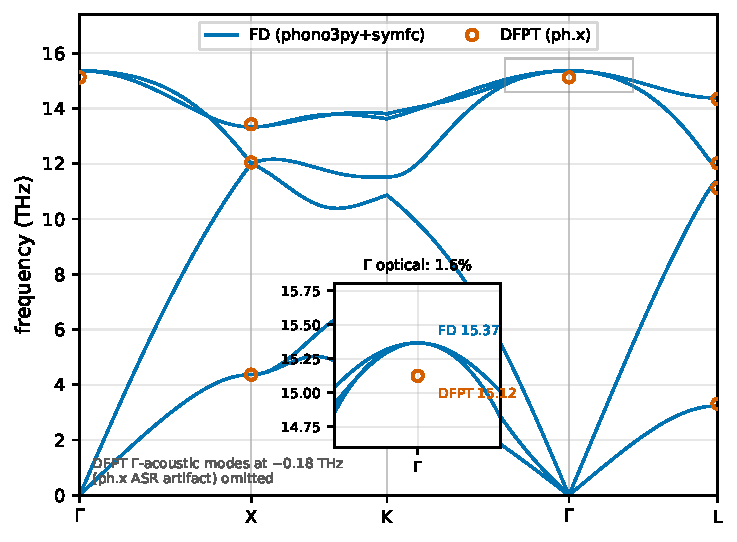
\includegraphics[width=0.6\linewidth]{transport_sweeps/fc_method_dispersion_si.pdf}
  \caption{Bulk-silicon phonon dispersion from DFPT versus
  finite-displacement force constants. The two \emph{ab-initio} methods
  agree to $1.6\%$ on the $\Gamma$ optical frequency.}
  \label{fig:res_fcmethod}
\end{figure}

\paragraph{Bulk-$\kappa$ anchor.} The finite-displacement FC3, fed to a
phono3py RTA-BTE calculation (natural isotopes), gives bulk-silicon
$\kappa(300\,\mathrm{K})=110.7$~W\,m$^{-1}$K$^{-1}$ on an $11^3$ mesh,
rising to $115.2$ on $19^3$. This is $\sim20$--$30\%$ below the
experimental $\sim150$, the known underestimate of a $2\times2\times2$
FC3 supercell (cutoff $5.5$~\AA); a larger supercell would close most of
the gap. This bulk $\kappa$ is the reference against which the
anharmonic self-energy prefactor should ultimately be benchmarked
(\cref{sec:res_prefactor}).

\paragraph{FC3 compression.} The decomposition machinery of
\cref{sec:fc3_compression} was applied to the $3\times3\times3$ silicon
FC3. The transport observable converges far faster than the Frobenius
residual: targeting a $1\%$ relative conductance error is reached by an
INDSCAL fit at rank $8$ ($117\times$ compression) while its Frobenius
residual is still $\sim17\%$, and the spectral heat-current curves are
visually indistinguishable from the dense reference by rank $16$. The
practical lesson is that the relevant fitting target for phonon NEGF is
a transport residual, not the Frobenius norm the fitters minimise.

% ======================================================================
\section{Anharmonic transport in silicon nanowires}
\label{sec:res_nw}
% ======================================================================

We study two hydrogen-passivated [100] silicon nanowires: \texttt{d5a}
($\mathrm{Si}_9\mathrm{H}_{12}$ per cell, $63$ DOF) and the wider
\texttt{d11a} ($135$ DOF). Their harmonic transport is clean
(\cref{fig:res_ballistic_curves}): the ballistic conductance rises with
temperature (thermal activation, saturating) and \texttt{d11a} carries
$\sim1.5\times$ the conductance of \texttt{d5a} (more channels). The
apparent decrease of $G$ with device length at finite broadening is the
$\eta$-induced coherence attenuation ($\ell\sim v_g/\eta_w$), not
diffusive resistance; the true Landauer plateau requires $\eta\to0$.

\begin{figure}[htb]
  \centering
  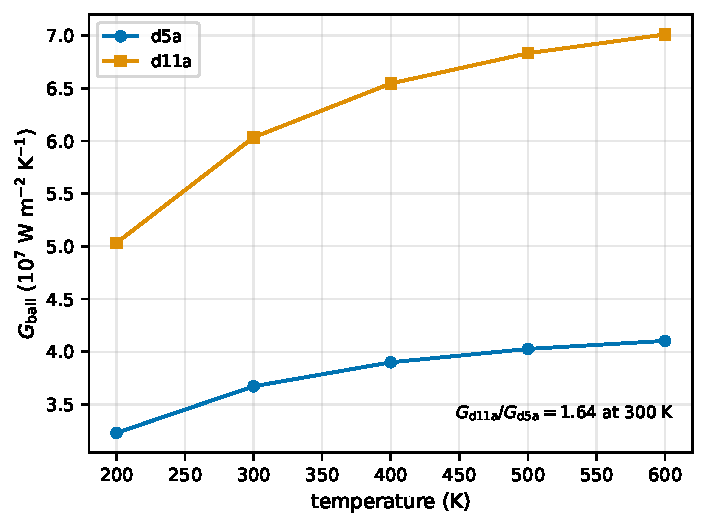
\includegraphics[width=0.48\linewidth]{transport_sweeps/ballistic_vs_T_d5_d11.pdf}\hfill
  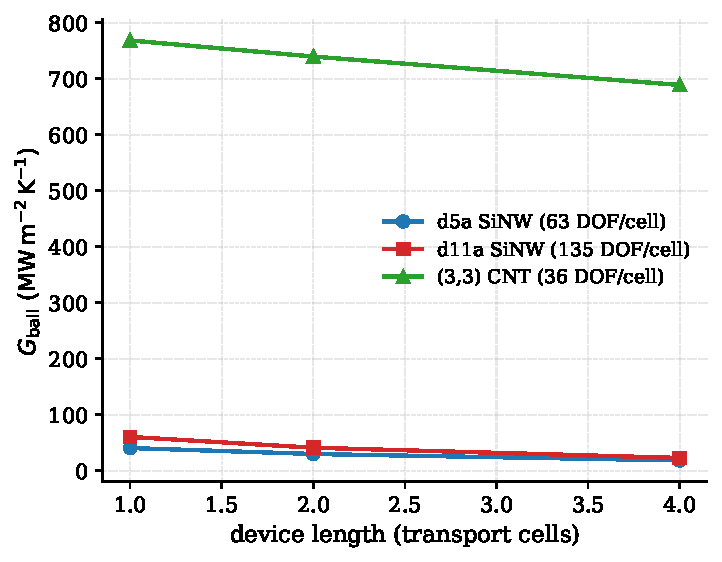
\includegraphics[width=0.48\linewidth]{transport_sweeps/ballistic_vs_length_d5_d11.pdf}
  \caption{Ballistic conductance of the \texttt{d5a} and \texttt{d11a}
  silicon nanowires. Left: $G(T)$; right: $G$ versus device length (the
  decrease is finite-$\eta$ coherence attenuation).}
  \label{fig:res_ballistic_curves}
\end{figure}

\paragraph{Mode-resolved anharmonic physics.} A phono3py analysis of the
bulk-silicon FC3 (\cref{fig:res_modephysics}) gives the context for the
nanowire results: phonon lifetimes have a median of $4.2$~ps with a
$\tau\!\propto\!\omega^{-2}$ envelope; $50\%$ of $\kappa$ is carried by
phonons with mean free path $>134$~nm and $93\%$ by acoustic modes;
Umklapp accounts for $0.44$ of the scattering at $300$~K; and the mode
Gr\"uneisen parameters have mean $|\gamma|=1.04$, matching the
experimental Si value and independently validating the FC3
\emph{anharmonicity strength}. Crucially, only $1.3\%$ of bulk
$\kappa$ comes from phonons with mean free path below $10$~nm. The
$\sim1$~nm nanowire cores therefore sit far below the bulk
phonon-MFP spectrum: they are \emph{boundary-scattering limited} and
retain almost none of the bulk anharmonic-limited $\kappa$. This is
why, at a single transport cell, the anharmonic correction to the
nanowire conductance is a small perturbation
($G_\mathrm{anh}/G_\mathrm{ball}\approx1$), and it is consistent across
the BTE-RTA and NEGF pictures.

\begin{figure}[htb]
  \centering
  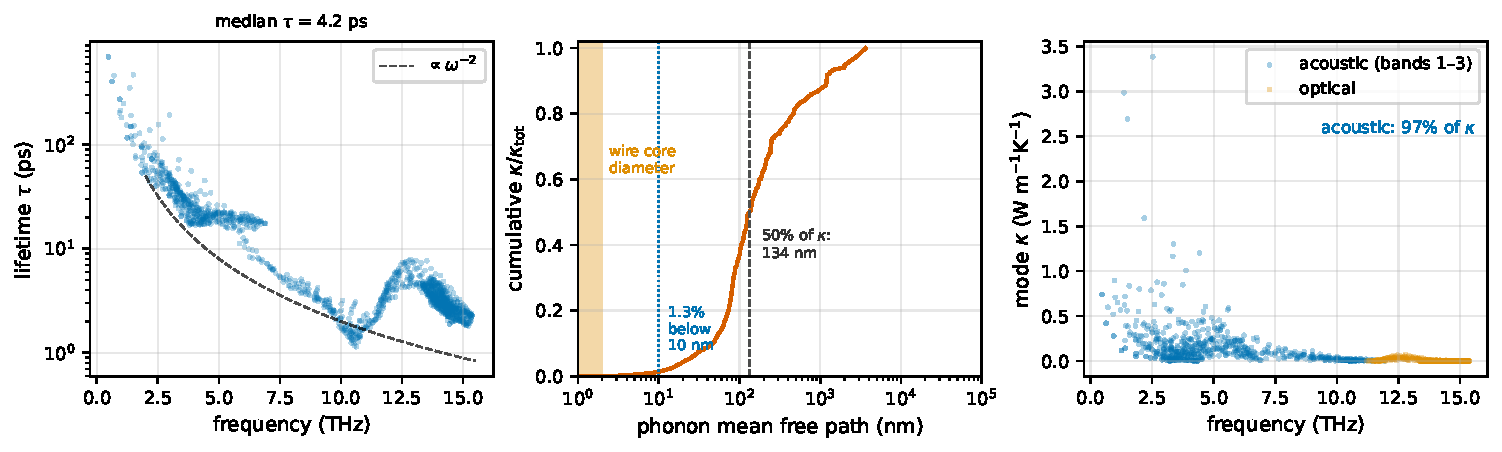
\includegraphics[width=0.48\linewidth]{transport_sweeps/phph_physics_si.pdf}\hfill
  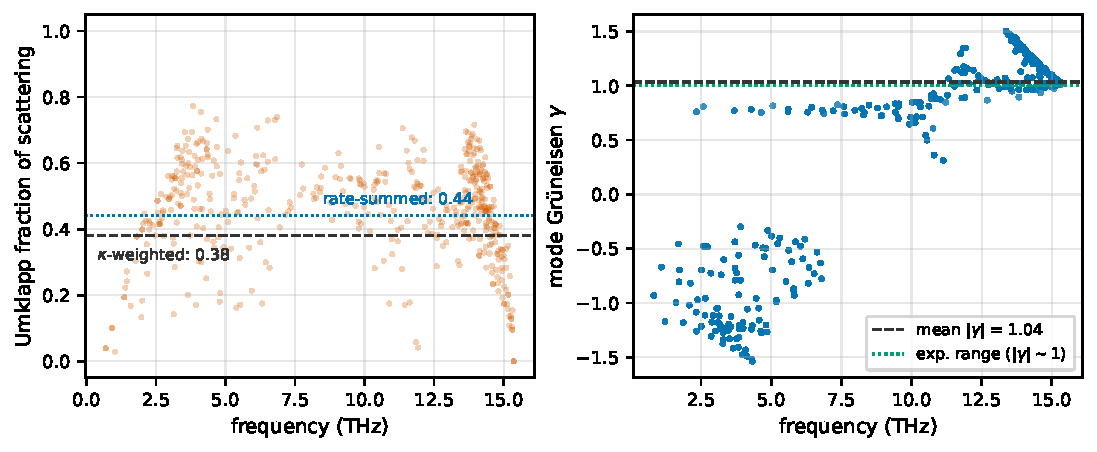
\includegraphics[width=0.48\linewidth]{transport_sweeps/phph_NU_gruneisen_si.pdf}
  \caption{Bulk-silicon mode-resolved anharmonic physics (phono3py,
  FD FC3). Left: lifetimes, $\kappa$-accumulation versus mean free path,
  and the acoustic-mode $\kappa$ fraction. Right: Normal/Umklapp split
  and the mode Gr\"uneisen distribution (mean $|\gamma|=1.04$).}
  \label{fig:res_modephysics}
\end{figure}

At physical broadening and moderate vertex strength the SCBA converges
cleanly and gives the physical $G_\mathrm{anh}<G_\mathrm{ball}$; the
soft-mode (\texttt{d5a} $0.027$~THz twist) and strong-coupling
behaviour, and the diagnosis that the original $\eta/\lambda$ sweep was
run at an unphysically large $\eta$, are documented in
\cref{app:convergence_diagnosis}.

% ======================================================================
\section{q-resolved anharmonic transport: silicon thin film}
\label{sec:res_qfilm}
% ======================================================================

For a transversely-periodic system the three-phonon self-energy couples
the transverse momenta by crystal-momentum conservation
(\cref{eq:sigma_q_dist}). As a quantitative benchmark we model
cross-plane heat transport through a silicon thin film following
Guo, Bescond and Zhang~\cite{guo_anharmonic_negf_2020}: the film is
bulk silicon truncated to $N$ layers along the transport direction with
in-plane two-dimensional periodicity, so it is exactly the
transverse-$q_\perp$ problem and reuses the \emph{bulk} silicon force
constants. The driver reduces to the $\Gamma$-only finite-device
transmission at a $1\times1$ mesh (checked automatically). Conductance
is reported per unit area, $G=J/(A_\perp\Delta T)$, and the cross-plane
conductivity of a film of thickness $L$ is $\kappa(L)=G\,L$.

\paragraph{Ballistic baseline.} The transverse mesh and broadening must
both be converged: at a fixed eight-layer thickness the ballistic
conductance converges for $8\times8$ or finer
($G_\mathrm{ball}=970/928/921/920$~MW\,m$^{-2}$K$^{-1}$ at
$4\times4/8\times8/12\times12/16\times16$), and a small $\eta$ is needed
to avoid the coherence attenuation of \cref{sec:res_nw} that otherwise
crushes the conductance. With these settings $G_\mathrm{ball}$ is nearly
thickness-independent ($\approx10^{3}$~MW\,m$^{-2}$K$^{-1}$) and the
ballistic $\kappa=G_\mathrm{ball}L$ rises essentially linearly with $L$
(\cref{fig:res_sifilm}, right) -- the non-intensive ballistic regime.
This ballistic conductance matches the scale of
Guo~\emph{et al.} to within a few percent.

\paragraph{Anharmonic conductance.} \Cref{fig:res_sifilm} (left)
compares our cross-plane conductance to the anharmonic-NEGF values of
Guo~\emph{et al.} at $3$ and $5$ unit cells. With the self-energy as
implemented (\emph{native} prefactor, \cref{sec:res_prefactor}) the
three-phonon scattering reduces the $3$-unit-cell conductance by
$\sim45\%$ ($G_\mathrm{anh}\approx570$~MW\,m$^{-2}$K$^{-1}$), markedly
more than the reference's $\sim10\%$
($G_\mathrm{anh}=939.7$). \emph{We have not resolved this
discrepancy}: it is either a transport-setup effect ($\eta$, mesh,
thin-device artifacts), the reference's additional approximations, the
difference in exchange--correlation functional of the underlying force
constants, or an absolute-prefactor error in the self-energy. The
second (green) curve in \cref{fig:res_sifilm} shows the effect of
scaling the vertex by one half (so $\Sigma\to\Sigma/4$); it moves the
conductance toward the reference ($831$ and $704$) but does not match
it, and we do \emph{not} claim it as a correction. The prefactor is
discussed honestly in \cref{sec:res_prefactor}.

\begin{figure}[htb]
  \centering
  
\includegraphics[width=0.92\linewidth]{transport_sweeps/si_film_conductance.pdf}
  \caption{Cross-plane heat transport through a silicon thin film at
  $300$~K with bulk-silicon force constants (transverse mesh $8\times8$,
  $121$ frequencies). \emph{Left}: per-area conductance versus
  thickness -- our ballistic and anharmonic NEGF against
  Guo~\emph{et al.}~\cite{guo_anharmonic_negf_2020}. The native
  self-energy over-scatters relative to the reference; the
  vertex-scaled curve illustrates the unresolved absolute prefactor
  (\cref{sec:res_prefactor}), and is not an established correction.
  \emph{Right}: the ballistic $\kappa=G_\mathrm{ball}L$ rises linearly
  with thickness (ballistic regime).}
  \label{fig:res_sifilm}
\end{figure}

% ======================================================================
\section{The three-phonon self-energy prefactor (open)}
\label{sec:res_prefactor}
% ======================================================================

The absolute scale of the anharmonic self-energy is, at the time of
writing, \textbf{not settled}, and we report it as an open issue rather
than a resolved one. The implemented kernel is the standard sunset
diagram (\cref{eq:sigma_guo}), which reduces analytically to the
correct Fermi-golden-rule three-phonon linewidth
(\cref{eq:fgr}). Against this, the silicon thin film over-scatters
relative to Guo~\emph{et al.} (\cref{sec:res_qfilm}), which would be
reconciled by a factor in the range $\sim2$--$4$ on the self-energy
(Guo~\emph{et al.} note a ``factor of four'' over-count of the repeated
internal pairings in the earlier Luisier convention). However, our
attempt to pin this factor independently against phono3py's
golden-rule linewidths for bulk silicon on the same FC3 is dominated by
the equilibrium-Green's-function normalisation: the broadening-free,
units-matched ratio
$\int(-\mathrm{Im}\,\Sigma^{\mathrm{NEGF}}_s)\,d\omega/\int 2\omega_s\,\gamma^{\mathrm{p3p}}_s\,d\omega$
comes out mode-independent and close to $(2\pi)^2$, i.e.\ a
normalisation/unit artifact of the standalone reconstruction rather than
a clean physical factor. The check therefore does not determine the
prefactor, and we have reverted to the unscaled (native) self-energy as
the default. The definitive, convention-free test -- bulk-silicon
$\kappa$ computed from the code's \emph{own} SCBA Green's functions and
compared to the phono3py RTA value of \cref{sec:res_fc} on the identical
FC3 -- is identified but not yet completed. All anharmonic conductances
in this chapter are quoted at the native prefactor and should be read
with this caveat.

% ======================================================================
\section{Full versus approximated self-energy}
\label{sec:res_approx}
% ======================================================================

The $q_\perp$-resolved transport driver computes, by construction, only
the slab-diagonal self-energy (the reference's ``diagonal-block''
approximation). We implemented the \emph{full} off-diagonal multi-slab
self-energy $\Sigma_{IJ}(q_\perp,\omega)$ -- which reduces exactly
(relative error $0$) to the $\Gamma$-only multi-slab self-energy at a
$1\times1$ mesh -- to measure each numerical approximation against the
unapproximated result. These ratios are prefactor-independent. For a
three-slab silicon film (first-Born step from the ballistic Green's
function): the off-diagonal self-energy blocks carry $47\%$ of the
Frobenius weight yet change the conductance by only $-1.8\%$, so the
diagonal-block approximation is well justified despite the blocks being
individually large; restricting the third-order vertex to the
nearest-neighbour slab shell changes the result by $<0.1\%$ (the
long-range FC3 is negligible, echoing the FC3-quality analysis); but
truncating the inter-slab \emph{Green's function} range gives an
unphysical (negative) conductance -- the off-diagonal $G$ coherence is
essential and must not be cut. Of the reference's numerical
approximations, the two it makes are benign at the few-percent level
here, while the Green's-function-range truncation, which it does
\emph{not} make, would be catastrophic.

% ======================================================================
\section{Silicon/germanium heterostructure}
\label{sec:res_hetero}
% ======================================================================

A Ge-layer barrier embedded in a silicon film (Si force constants,
Ge mass; Si contacts) is built with a per-slab mass profile threaded
through the $q_\perp$-resolved driver (an all-Si profile reproduces the
homogeneous driver to machine precision). The mass-mismatch barrier
raises the \emph{ballistic} thermal resistance by $+340$--$370\%$
(harmonic interface reflection). The phonon-phonon enhancement of the
resistance is present in the pure silicon film -- $+32\%$ at $2.3$~nm
growing to $+51\%$ at $5.4$~nm (the anharmonic resistance accumulates
with thickness, the diffusive crossover) -- but is suppressed
($\lesssim1\%$) in the barrier-dominated heterostructure, because the
strong mass barrier filters transmission to low-frequency acoustic
phonons that are anharmonically long-lived. (The magnitude of the
anharmonic enhancement inherits the prefactor caveat of
\cref{sec:res_prefactor}; the barrier reflection and the qualitative
filtering picture do not.)

% ======================================================================
\section{Distributed solver and self-energy; GPU memory}
\label{sec:res_scaling}
% ======================================================================

\paragraph{Dyson solve.} The block-tridiagonal recursive Green's
function (RGF) solve is linear in the number of transport cells while
the dense reference is cubic ($57\times$ apart at $32$ blocks, agreeing
to $\sim10^{-13}$; \cref{fig:res_solver}, left). Distributing the energy
points across MPI ranks gives $5.3\times$ at eight ranks
(\cref{fig:res_solver}, right) -- the Dyson solve is
energy-embarrassingly-parallel.

\begin{figure}[htb]
  \centering
  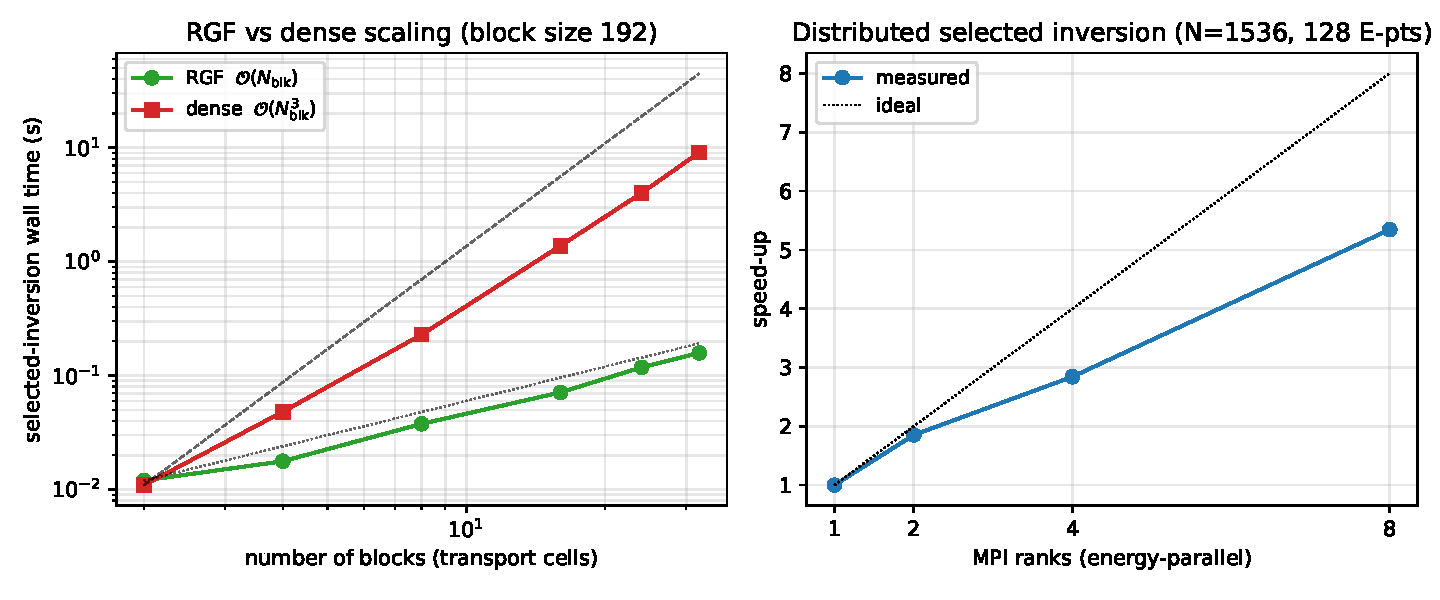
\includegraphics[width=0.48\linewidth]{transport_sweeps/solver_scaling.pdf}\hfill
  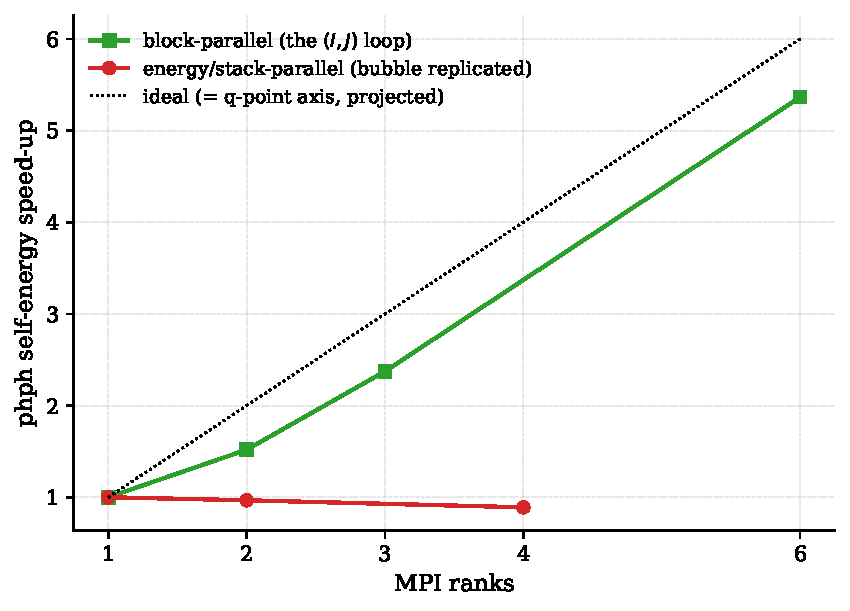
\includegraphics[width=0.48\linewidth]{transport_sweeps/phph_scaling.pdf}
  \caption{Left: solver scaling -- RGF (linear) versus dense
  selected-inversion (cubic), and the energy-parallel speed-up
  ($5.3\times$ at eight ranks). Right: distributed scaling of the
  production three-phonon self-energy -- the spatial-block
  $(I,J)$ axis is near-ideal while the energy axis is flat because the
  energy convolution is replicated (\cref{ssec:phph_distribution}).}
  \label{fig:res_solver}
\end{figure}

\paragraph{Self-energy.} The production phonon-phonon self-energy
parallelises near-ideally over the spatial-block axis ($1.0/1.52/2.37/5.36\times$
at $1/2/3/6$ ranks) but is flat over the energy axis: the bubble is an
energy convolution that couples all frequencies, so each stack rank
recomputes the full-frequency FFT and writes only its slice
(\cref{fig:res_solver}, right).

\paragraph{Transverse-momentum axis.} The dedicated $q$-communicator of
\cref{ssec:phph_qdist} -- distributing the external $q_\perp$ and
all-gathering the internal-momentum Green's functions -- scales
near-ideally: $1.0/1.87/3.58/6.58\times$ at $1/2/4/8$ ranks
($82\%$ efficiency), with the self-energy bit-identical across rank
counts (\cref{fig:res_qscaling}, left). This is the scalable axis for
the periodic anharmonic problem, in contrast to the replicated energy
axis.

\paragraph{GPU memory.} For the periodic problem the binding constraint
is memory: the dense Fourier vertex $\tilde\Phi(q_\perp,q_\perp')$ scales
as $\cO(N_q^2\,\ndof^3)$ (16~GB already at an $8\times8$ mesh and
wire-scale cross section). Streaming it from the gathering matrices and
the real-space FC3 (\cref{ssec:phph_qdist}) drops the peak to
$\cO(N_q\,\ndof^2)$ (\cref{fig:res_qscaling}, right), bit-identical to
the dense path, and composes with the $q$-communicator at no extra
communication.

\begin{figure}[htb]
  \centering
  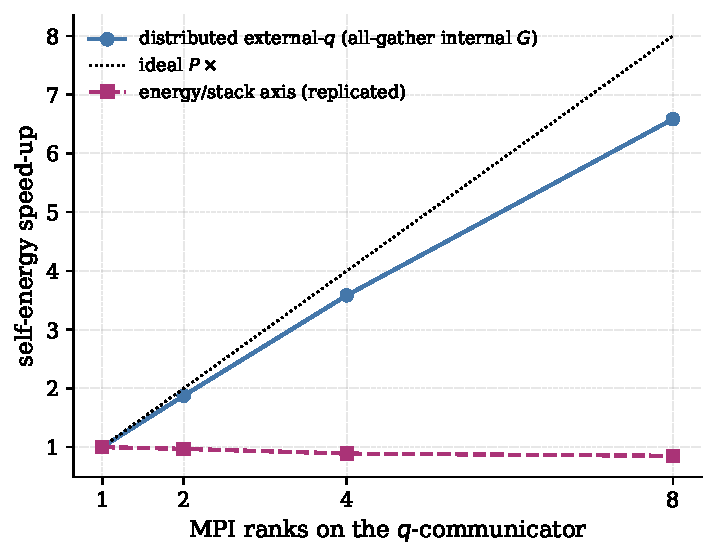
\includegraphics[width=0.48\linewidth]{transport_sweeps/phph_q_scaling.pdf}\hfill
  
\includegraphics[width=0.48\linewidth]{transport_sweeps/phph_memory.pdf}
  \caption{Left: distributed scaling of the $q_\perp$-resolved
  three-phonon self-energy over the $q$-communicator (near-ideal;
  self-energy bit-identical across ranks). Right: peak memory of the
  momentum-space vertex -- dense $\cO(N_q^2\ndof^3)$ versus streamed
  $\cO(N_q\ndof^2)$ (the star is a measured value).}
  \label{fig:res_qscaling}
\end{figure}

% ======================================================================
\section{Cutoff hierarchy and transport sensitivity}
\label{sec:res_cutoffs}
% ======================================================================

A self-energy-level cutoff sweep on the \texttt{d5a} and \texttt{d11a}
nanowires (\cref{fig:res_cutoffs}) quantifies the truncations: the FC3
magnitude threshold converges quickly for \texttt{d5a}
($10^{-3}\to0.7\%$ relative change in $\Sigma^<$) but the wider
\texttt{d11a} needs a tighter threshold (it has more small-but-relevant
vertex elements), whereas a diagonal-$G$ approximation inside the bubble
is catastrophic ($5\times$ for \texttt{d5a}, $30\times$ for
\texttt{d11a}). The dominant cutoff is the Green's-function range, not
the vertex magnitude -- consistent with the q-resolved finding of
\cref{sec:res_approx} that the inter-slab $G$ coherence must be kept.

\begin{figure}[htb]
  \centering
  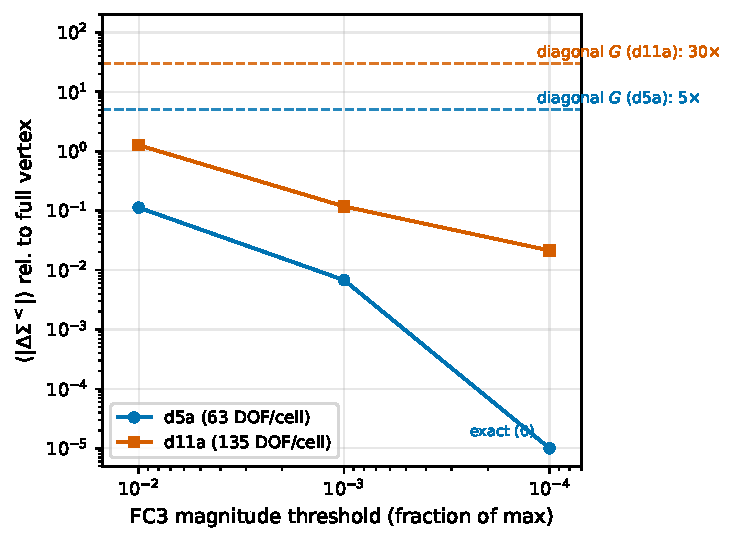
\includegraphics[width=0.6\linewidth]{transport_sweeps/cutoff_sse_d5_d11.pdf}
  \caption{Self-energy sensitivity to the FC3 magnitude cutoff and to a
  diagonal-$G$ approximation for the \texttt{d5a} and \texttt{d11a}
  nanowires. The off-diagonal Green's-function content dominates.}
  \label{fig:res_cutoffs}
\end{figure}


\appendix

\chapter{Conventions and Units}
\label{ch:conventions_units}

This chapter collects the unit systems, notation, and Fourier
conventions used in this document.  The harmonic force
constants may originate either from phonopy finite-displacement
calculations or from Quantum ESPRESSO (QE) density-functional
perturbation theory, while the QuaTrEx solver uses its own internal
frequency-squared convention.  Since the later extraction, transport,
and anharmonic self-energy steps all rely on consistent units and phase
conventions, we summarize them here once and refer back to this section
% REVIEW: this file IS the chapter; refer to the document, not the chapter
throughout the document.

% ----------------------------------------------------------------------
\section{Units in phonopy and Quantum ESPRESSO}
\label{sec:phonopy_units}
% ----------------------------------------------------------------------

Phonopy stores force constants in eV/\AA$^2$, atomic masses in amu, and
atomic positions in \AA.  The dynamical matrix eigenvalues therefore
have units
\begin{equation}
  [\lambda] = \frac{\mathrm{eV}}{\mathrm{amu}\cdot\mathrm{\si{\angstrom}}^2}.
\end{equation}
Phonopy converts these eigenvalues to frequencies in THz via
% REVIEW: the appended ~15.633 THz is the VaspToTHz prefactor alone (lambda-independent), not the value of f
\begin{equation}\label{eq:VaspToTHz}
  f\;[\mathrm{THz}]
  = \mathrm{sgn}(\lambda)\,\sqrt{|\lambda|}
    \times
    \frac{1}{2\pi}\sqrt{\frac{e}{m_u A^2}}  \approx 15.633\;\mathrm{THz},
\end{equation}
where $e = 1.602\times 10^{-19}$\,J is the elementary charge,
$m_u = 1.661\times 10^{-27}$\,kg is the atomic mass unit, and
% REVIEW: 1e-10 m is the Angstrom-to-metre factor, not metre-to-Angstrom
$A = 10^{-10}$\,m is the \AA-to-metre conversion factor.

When phonopy is used together with the QE interface, the internal
representation inherited from QE uses atomic units: lattice vectors are
in bohr and force constants in Ry/bohr$^2$.  These quantities are
therefore converted before being used together with the rest of the
workflow.  The required relations are
\begin{align}
  a\;[\mathrm{\si{\angstrom}}]
    &= a\;[\mathrm{bohr}] \times a_0,
    & a_0 &= 0.52918\;\mathrm{\si{\angstrom}/bohr}, \\
  \Phi\;[\mathrm{eV/\si{\angstrom}^2}]
    &= \Phi\;[\mathrm{Ry/bohr^2}] \times \frac{E_h/2}{a_0^2},
    & \frac{E_h/2}{a_0^2} &\approx 48.59.
\end{align}
Here $E_h$ denotes the Hartree energy, so that $E_h/2 = 1$\,Ry.  In the
same way, Cartesian forces parsed from QE output are converted using
\begin{equation}
  1\;\mathrm{Ry/bohr} \approx 25.711\;\mathrm{eV/\si{\angstrom}}.
\end{equation}

The downstream workflow therefore treats eV, \AA, and amu as the common
intermediate unit system, independent of whether the original data came
from phonopy directly or through QE.  In other words, everything is
normalized to the phonopy eV/\AA/amu convention upon loading.

% ----------------------------------------------------------------------
\section{QuaTrEx solver units}
\label{sec:solver_units}
% ----------------------------------------------------------------------

The QuaTrEx phonon solver operates in angular frequency squared,
\begin{equation}
  \omega^2 \quad \text{in} \quad (\mathrm{rad/s})^2.
\end{equation}
Accordingly, the mass-weighted real-space blocks passed to the solver
must be converted from the phonopy eigenvalue units
eV/(amu$\cdot$\AA$^2$) to $(\mathrm{rad/s})^2$.  The corresponding
conversion factor is
\begin{equation}\label{eq:conversion}
  C = \frac{e}{m_u A^2}
  \approx 9.648 \times 10^{27}\;\mathrm{(rad/s)^2}.
\end{equation}
If $\Phi(0,\vc{R})$ denotes a harmonic force-constant block in
eV/\AA$^2$, then the real-space matrix block used by QuaTrEx is
\begin{equation}
  H(\vc{R})
  = C\,
    \frac{\Phi(0,\vc{R})}{\sqrt{m\,m'}},
\end{equation}
with $m$ and $m'$ in amu.  The resulting $H(\vc{R})$ therefore has units
of $(\mathrm{rad/s})^2$.

The same logic extends to cubic force constants.  After mass-weighting,
the third-order tensor
\begin{equation}
  \Psi_{\alpha\beta\gamma}
  = \frac{\Phi^{(3)}_{\alpha\beta\gamma}}
         {\sqrt{M_\kappa M_{\kappa'} M_{\kappa''}}}
\end{equation}
has units
\begin{equation}
  [\Psi] = \frac{\mathrm{eV}}
                 {\mathrm{\si{\angstrom}}^3\cdot\mathrm{amu}^{3/2}}.
\end{equation}
Its SI conversion factor is
\begin{equation}\label{eq:conversion_fc3}
  \texttt{CONVERSION\_FC3}
  = \frac{C}{A\sqrt{m_u}}
  = \frac{e}{m_u^{3/2} A^3}
  \approx 2.368\times10^{51},
\end{equation}
which converts
eV/(\AA$^3\cdot$amu$^{3/2}$) to the SI units required in the
phonon--phonon self-energy expressions.

% REVIEW: code->doc -- the production phonon-phonon stack (quatrex/phonon/units.py; static_self_energy.py device_fc3_mass_weighted; bubble_prefactor_thz = i*hbar*dOmega/(4 pi)) actually runs in a THz^2 / plain-THz internal system, not (rad/s)^2; reconcile
\paragraph{THz-based internal unit system.}
The $(\mathrm{rad/s})^2$ statement above is the SI-facing equivalent.  In
practice the production phonon--phonon stack
(\texttt{quatrex/phonon/units.py},
\texttt{static\_self\_energy.py:\,device\_fc3\_mass\_weighted}) works in a
\emph{THz-based} internal system: the dynamical matrix $D$ and all
self-energies are carried in $\mathrm{THz}^2$, while the frequency axis
$\omega$ is in plain THz, with the bubble assembled using
$\texttt{bubble\_prefactor\_thz} = i\hbar\,\Delta\Omega/(4\pi)$.  The
$\mathrm{THz}^2$ convention and this prefactor are documented in
\cref{ap:fa_overview}; the $(\mathrm{rad/s})^2$ form and
\cref{eq:conversion_fc3} provide the SI-facing equivalents.

\paragraph{Green's-function sign convention.}
% REVIEW: labeling tension -- theory/30_scba_eta0.tex and infrared.tex write G^<_eq=-i n A (textbook sign) while invoking "occupation-positive"; the stored solver sign is +i n A. Those two appendix statements should cite the textbook sign G^<=-inA explicitly. (FLAG-ONLY: no math changed here.)
The solver stores the phonon Green's functions and self-energies
\emph{occupation-positive}: $-iG^{\lessgtr}(\omega)\succeq0$ for $\omega>0$, the
same sign as the lead injection
$\Sigma_\ell^{\lessgtr}=+i\,n_\ell(\pm1)\Gamma_\ell$. This differs from the
common textbook choice $G^<=-i\,nA$ by an overall sign of $G^{\lessgtr}$ --- and
hence of any self-energy quadratic in $G$, such as the three-phonon bubble; see
the remark following \cref{eq:sigma_r} for the consequent sign handling.

% ----------------------------------------------------------------------
\section{Notation and Fourier conventions}
\label{sec:notation_fourier}
% ----------------------------------------------------------------------

We first collect the symbols used throughout this work.

\begin{center}
\begin{tabular}{llr}
  \toprule
  Symbol & Meaning & Range \\
  \midrule
  $l,m$                              & Supercell index                              & $\Ncell$ \\
  $\kappa,\kappa',\kappa''$          & Basis-atom within a primitive cell            & $\nprim$ \\
  $\alpha,\alpha',\alpha''$          & Cartesian component ($x,y,z$)                & $C=3$ \\
  $i, j, k$                          & DOF index                                    & $\ndof$ \\
  $\mu, \nu$                         & Primitive-cell DOF index                     & $3\nprim$ \\
  $\vq_\perp$                        & Transverse wavevector (2D BZ)                & $N_q$ points \\
  $x,y$                              & Transport-direction DOF                      & $\ntrans = 3\nprim N_\mathrm{transport}$ \\
  $\vR_\perp$                        & Transverse lattice vector                    & $N_q$ points (dual) \\
  $\omega,\omega'$                   & Real frequency                               & $N_\omega$ points \\
  $\tau$                             & Conjugate time variable                      & $N_\tau = N_\omega$ \\
  $N$                                & Total number of $\vq$-points, $N_q$          & \\
  \bottomrule
\end{tabular}
\end{center}

Here $\Ncell$ is the total number of supercells (e.g.\ $3^3 = 27$),
$\nprim$ the number of atoms in the primitive cell (e.g.\ $2$ for
bulk Si), and
% REVIEW: Ncell is the TOTAL cell count (=27), so total DOF = 3 Ncell nprim; drop the spurious cube
$\ndof = 3\nsuper = 3\Ncell\nprim$ the total number of degrees of
freedom in the simulation.  $\ntrans$ is the total number of DOFs in
the transport direction (i.e.\ when transverse cells are not
included), and $N_\mathrm{transport}$ is the number of transport
(super)-cells.

Bold symbols such as $\vR$ and $\vq$ denote lattice vectors and
wavevectors, respectively.  The displacement of atom $\kappa$ in
cell $l$ along direction $\alpha$ is written $u_\alpha(l\kappa)$.
The lattice vector of cell $l$ is $\vR_l$, while $\vc{\tau}_\kappa$
denotes the basis-atom position within the unit cell.  Unless stated
otherwise, $\vc{\tau}_\kappa$ and $\vq$ are expressed in fractional
% REVIEW: two phase conventions actually coexist; the blanket "2pi in all phases" claim contradicts eq:dft_fwd/eq:dft_inv -- state both explicitly
crystal coordinates.  Two distinct phase conventions are used in this
work: the dynamical-matrix transforms
(\cref{eq:DA_conv,eq:DB_conv,eq:fourier_series_conv}) carry an explicit
$2\pi$, i.e.\ $e^{+2\pi i\,\vq\cdot\vR}$, whereas the
Green's-function/self-energy discrete Fourier pair
(\cref{eq:dft_fwd,eq:dft_inv}) absorbs the $2\pi$ into $\vq$ and uses the
opposite forward sign, $e^{-i\,\vq\cdot\vR}$.

The harmonic force constants are written as
\begin{equation}
  \Phi_{\alpha\alpha'}(0\kappa,\,l'\kappa'),
\end{equation}
and the corresponding mass-weighted dynamical matrix at wavevector
$\vq$ is a Fourier transform of these real-space couplings.
Two phase conventions are used in this work.  In the phonopy
convention,
\begin{equation}\label{eq:DA_conv}
  D_{\alpha\alpha'}^{(\mathrm{A})}(\kappa\kappa',\vq)
  = \frac{1}{\sqrt{m_\kappa m_{\kappa'}}}
    \sum_{l'} \Phi_{\alpha\alpha'}(0\kappa,\,l'\kappa')\,
    e^{2\pi i\,\vq\cdot
      [\vR_{l'} + \vc{\tau}_{\kappa'} - \vc{\tau}_\kappa]},
\end{equation}
whereas the QuaTrEx convention uses only the lattice vector in the
phase,
\begin{equation}\label{eq:DB_conv}
  D_{\alpha\alpha'}^{(\mathrm{B})}(\kappa\kappa',\vq)
  = \frac{1}{\sqrt{m_\kappa m_{\kappa'}}}
    \sum_{l'} \Phi_{\alpha\alpha'}(0\kappa,\,l'\kappa')\,
    e^{2\pi i\,\vq\cdot\vR_{l'}}.
\end{equation}
The two are related by a diagonal unitary gauge transformation,
\begin{equation}\label{eq:gauge_conv}
  D^{(\mathrm{B})}(\vq)
  = P(\vq)\,D^{(\mathrm{A})}(\vq)\,P^\dagger(\vq),
\end{equation}
with
\begin{equation}
  P(\vq)_{\kappa\alpha,\kappa'\alpha'}
  = \delta_{\kappa\kappa'}\delta_{\alpha\alpha'}\,
    e^{2\pi i\,\vq\cdot\vc{\tau}_\kappa}.
\end{equation}
Under Convention~B, the dynamical matrix is a pure lattice Fourier
series,
\begin{equation}\label{eq:fourier_series_conv}
  D^{(\mathrm{B})}(\vq)
  = \sum_{\vR} H(\vR)\,e^{2\pi i\,\vq\cdot\vR}.
\end{equation}
% REVIEW: symbol overloading -- H(R) here is the (rad/s)^2 block of eq:conversion (= C*Phi/sqrt(mm')), i.e. it carries the C conversion, unlike the bare mass-weighted Phi/sqrt(mm') used in eq:DB_conv
Here $H(\vR)$ is the SI-converted mass-weighted block introduced in
\cref{eq:conversion}, $H(\vR) = C\,\Phi(0,\vR)/\sqrt{m\,m'}$, so that it
already carries the conversion factor $C$; the $D^{(\mathrm{B})}$ of
\cref{eq:DB_conv} instead uses the bare mass-weighted force constants
$\Phi/\sqrt{m_\kappa m_{\kappa'}}$ and therefore differs from
\cref{eq:fourier_series_conv} by the overall factor $C$.

For the transverse directions we write $\vq_\perp$ for the
two-dimensional transverse wavevector.  A partial Fourier sum over
transverse lattice vectors $\vR_\perp$ then takes the form
\begin{equation}
  D(\vq_\perp)
  = \sum_{\vR_\perp} M(\vR_\perp)\,
    e^{2\pi i\,\vq_\perp\cdot\vR_\perp}.
\end{equation}
The transverse wavevectors are sampled on a Monkhorst--Pack mesh,
\begin{equation}
  q_{\perp,i} = \frac{n_i + 0.5}{N_i} - 0.5 + \mathrm{shift}_i,
  \qquad n_i = 0,\ldots,N_i-1.
\end{equation}

We also define the discrete Fourier-transform pair
\begin{align}
  G(\omega;\vq) &= \sum_{\vR} g(\omega;\vR)\,e^{-i\vq\cdot\vR},
  \label{eq:dft_fwd} \\
  g(\omega;\vR) &= \frac{1}{N}\sum_{\vq} G(\omega;\vq)\,e^{+i\vq\cdot\vR},
  \label{eq:dft_inv}
\end{align}
with the associated discrete convolution theorem
\begin{equation}\label{eq:conv_theorem}
  \frac{1}{N}\sum_{\vq'} A(\vq')\,B(\vq-\vq')
  = \sum_{\vR} a(\vR)\,b(\vR)\,e^{-i\vq\cdot\vR}.
\end{equation}
\chapter{Quatrex Documentation}
\label{ch:quatrex_doc}

% ----------------------------------------------------------------------
\subsection{QuaTrEx Input format}
\label{sec:quatrex_input}
% ----------------------------------------------------------------------

The QuaTrEx solver reads three input files which
specify the real-space Hamiltonian, the crystal structure, and the
transport parameters.

\subsubsection{Input files}
\label{sec:input_files}

\paragraph{\texttt{dynamical\_matrix.mat}}
This MATLAB \texttt{.mat} file stores the real-space blocks
$H(\vc{R})$ in Convention~B, already converted to
$(\mathrm{rad/s})^2$.  Each block is stored under a string key of the
form
\begin{equation}
  \texttt{"[nx, ny, nz]"},
\end{equation}
mapping to a real matrix of dimension
$(n_\mathrm{dof}\times n_\mathrm{dof})$, where
$n_\mathrm{dof}=3N_b$ and $N_b$ is the number of atoms in the unit
cell.  For nearest-neighbour interactions extracted on a
$3\times3\times3$ mesh, the file contains up to 27 blocks.

The solver interprets these blocks as real-space couplings and, for
periodic transverse directions, performs the Fourier sum
\begin{equation}
  D(\vc{k}_\perp)
  = \sum_{(n_x,n_y)} M(n_x,n_y)\;
    e^{2\pi i\,(k_x n_x + k_y n_y)}.
\end{equation}

\paragraph{\texttt{structure.xyz}}
This is an extended XYZ file containing the lattice vectors in the
header and Cartesian atomic positions in the body.  It follows the ASE
extended-XYZ convention, for example
\begin{verbatim}
8
Lattice="5.4018 0.0 0.0 0.0 5.4018 0.0 0.0 0.0 5.4018" ...
Si  0.00000000  0.00000000  0.00000000
...
\end{verbatim}
The loader (\texttt{distributed\_read\_xyz}) extracts the $3\times3$
lattice matrix and Cartesian atom positions.  The number of atoms times
\texttt{num\_orbitals\_per\_atom} determines $n_\mathrm{dof}$.

\paragraph{\texttt{quatrex\_config.toml}}
This file specifies the transport setup, such as transport direction,
number of transport cells, neighbour cutoff, transverse $k$-mesh,
broadening, and the open-boundary-condition algorithm.  Important fields are
\begin{center}
\begin{tabular}{lll}
  \toprule
  Field & Example value & Purpose \\
  \midrule
  \texttt{transport\_direction}       & \texttt{'z'}            & transport axis \\
  \texttt{construct\_from\_unit\_cell}& \texttt{true}           & input mode selector \\
  \texttt{num\_transport\_cells}      & 4                       & device length in unit cells \\
  \texttt{neighbor\_cell\_cutoff}     & \texttt{[1,1,1]}        & block-range cutoff \\
  \texttt{kpoint\_grid}               & \texttt{[4,4,1]}        & transverse mesh \\
  \texttt{kpoint\_shift}              & \texttt{[0,0,0]}        & Monkhorst--Pack shift \\
  \texttt{num\_orbitals\_per\_atom.Si}& 3                       & DOFs per atom \\
  \texttt{phonon.eta}                 & \texttt{1e-8}           & broadening $(\mathrm{rad/s})^2$ \\
  \texttt{phonon.obc.algorithm}       & \texttt{"sancho-rubio"} & OBC method \\
  \bottomrule
\end{tabular}
\end{center}

\subsubsection{Input modes}
\label{sec:input_modes}

QuaTrEx supports two input modes, selected by
\texttt{construct\_from\_unit\_cell}.  In both modes the input is a
MATLAB \texttt{.mat} file loaded by \texttt{scipy.io.loadmat}.  The
loader (\\\texttt{distributed\_load} in
\texttt{qttools/utils/mpi\_utils.py}) parses keys that start with
\texttt{[} and interprets them as integer tuples:
\begin{lstlisting}
arr = loadmat(path)
arr = {
    tuple(map(int, r.strip("[]").split(","))): h_r
    for r, h_r in arr.items()
    if r.startswith("[")
}
\end{lstlisting}
That is, a key string such as \texttt{"[0, 1, -1]"} becomes the Python
tuple \texttt{(0, 1, -1)}.  Each value is a 2D NumPy array (real or
complex) representing a matrix block.

\paragraph{Mode 1: pre-assembled device matrix}
If \texttt{construct\_from\_unit\_cell = false}, the
\texttt{dynamical\_matrix.mat} file contains a single pre-assembled
device matrix stored under the key \texttt{(0,0,0)}:
\begin{lstlisting}
matrix_sparray = distributed_load(f"{matrix_name}.mat")
assert (0, 0, 0) in matrix_sparray.keys()
matrix_sparray = matrix_sparray[(0, 0, 0)]
\end{lstlisting}
The result is a single sparse matrix of size
$(N_\mathrm{blocks}\times B)^2$, where $B$ is the block size and
$N_\mathrm{blocks}$ is the number of transport cells.  No transverse
$k$-point Fourier assembly is performed.

\paragraph{Mode 2: unit-cell blocks}
If \texttt{construct\_from\_unit\_cell = true}, the file contains the
dictionary of real-space unit-cell blocks
$H(n_x,n_y,n_z)$.  The solver loads all blocks, constructs a dense
translation grid, optionally trims it using
\texttt{neighbor\_cell\_cutoff}, expands the blocks into
transport-direction BTD matrices, and performs the transverse
Fourier assembly on the chosen Monkhorst--Pack mesh.

The function \texttt{\_load\_matrix\_from\_unit\_cell} loads all keys,
determines the bounding box from the minimum and maximum key
coordinates, and packs the blocks into a 5D array:
\begin{lstlisting}
# keys: array of all (nx, ny, nz) tuples
min_coords = keys.min(axis=0)
max_coords = keys.max(axis=0)
grid_shape = max_coords - min_coords + 1
unit_cells = zeros(grid_shape + matrix_shape)
for coord, matrix in matrices.items():
    unit_cells[coord] = matrix
\end{lstlisting}
The resulting array has shape
$(G_x,G_y,G_z,n_\mathrm{dof},n_\mathrm{dof})$, where
$(G_x,G_y,G_z)$ is the grid shape (e.g.\ $(3,3,3)$ for
$\{-1,0,+1\}^3$).  The loader checks that
$G_x \times G_y \times G_z = \text{number of keys}$, i.e.\ the grid
must be dense: no missing entries are permitted.  Missing blocks must
be stored as zero matrices.

If \texttt{neighbor\_cell\_cutoff} is set (e.g.\ \texttt{[1,1,1]}),
\texttt{trim\_tight\_binding\_matrix} zeros out all blocks beyond that
range.  For cutoff $(c_x,c_y,c_z)$, a block at index
$(n_x,n_y,n_z)$ (centred at zero) is kept only if
$|n_x| \le c_x$, $|n_y| \le c_y$, $|n_z| \le c_z$.

The function \texttt{expand\_tight\_binding\_matrix} converts the
unit-cell blocks into a BTD sparse matrix for a given transverse
periodic shift.  Along the transport direction $z$:
\begin{enumerate}
  \item The supercell size in the transport direction is $G_z / 2$
        (integer division), and 1 in the transverse directions.  For
        $G_z = 3$, this gives a supercell of one unit cell
        ($3 // 2 = 1$).
  \item Three BTD blocks are extracted for each transverse periodic
        shift $(n_x,n_y)$:
        \begin{itemize}
          \item $n_z=-1$: lower off-diagonal,
          \item $n_z=0$: diagonal,
          \item $n_z=+1$: upper off-diagonal.
        \end{itemize}
  \item Each block is assembled by \texttt{\_get\_transport\_block},
        which loops over all pairs of local shifts within the supercell
        and selects the appropriate unit-cell block for each pair.
  \item The three blocks are tiled $N_\text{transport}$ times along the
        diagonal to build the full BTD sparse matrix.
\end{enumerate}

The function \texttt{\_assemble\_kpoint} then performs the Fourier sum
over transverse periodic shifts.  For each $\vc{k}_\perp$ on a
Monkhorst--Pack mesh:
\begin{equation}\label{eq:assemble}
  D(\vc{k}_\perp)
  = \sum_{(n_x,n_y)} M(n_x,n_y)\;
    e^{2\pi i\,(k_x n_x + k_y n_y)},
\end{equation}
where $M(n_x,n_y)$ is the BTD sparse matrix for periodic shift
$(n_x,n_y)$, already expanded in the transport direction.  The
$k$-points on the Monkhorst--Pack mesh are
\begin{equation}
  k_i = \frac{n_i + 0.5}{N_i} - 0.5 + \text{shift}_i,
  \qquad n_i = 0,\ldots,N_i-1.
\end{equation}
The result is a stack of BTD matrices indexed by
$(\omega,k_x,k_y)$.

% ----------------------------------------------------------------------
\subsection{Heterogeneous-device extension}
\label{sec:heterogeneous}
% ----------------------------------------------------------------------

The original harmonic unit-cell input mode in QuaTrEx constructs a
homogeneous device by repeating the same block set across all transport
cells.  To model interfaces such as Si/Ge, the harmonic assembly was
extended to support piecewise-defined left, device, and right regions
with distinct block dictionaries.

\subsubsection{L|D|R device model}

The transport region is partitioned into three sections,
\begin{equation}\label{eq:ldr}
  \underbrace{L\;\cdots\;L}_{n_L\;\text{cells}}
  \;\underbrace{D\;\cdots\;D}_{n_D\;\text{cells}}
  \;\underbrace{R\;\cdots\;R}_{n_R\;\text{cells}},
  \qquad
  n_L + n_D + n_R = n_\mathrm{transport},
\end{equation}
where the left and right parts serve as lead-like material regions and
the central part represents the interface or device region.

\subsubsection{Configuration changes}

To support this heterogeneous harmonic setup, four new configuration
fields were added to \texttt{DeviceConfig}:
\begin{center}
\begin{tabular}{lll}
  \toprule
  Field & Type & Purpose \\
  \midrule
  \texttt{num\_left\_cells}  & \texttt{PositiveInt | None} & number of left cells $n_L$ \\
  \texttt{num\_right\_cells} & \texttt{PositiveInt | None} & number of right cells $n_R$ \\
  \texttt{left\_matrix}      & \texttt{str | None}         & left-lead \texttt{.mat} file \\
  \texttt{right\_matrix}     & \texttt{str | None}         & right-lead \texttt{.mat} file \\
  \bottomrule
\end{tabular}
\end{center}
This mode requires
\texttt{construct\_from\_unit\_cell = true} and must satisfy
\begin{equation}
  n_L + n_R < n_\mathrm{transport},
\end{equation}
so that at least one transport cell remains in the device region.

\subsubsection{Matrix assembly}

The heterogeneous assembly is implemented by extending the harmonic
unit-cell expansion to allow different block dictionaries in different
transport cells.  Two new functions were added to
\texttt{quatrex/device/inputs.py}.

\texttt{\_expand\_heterogeneous\_matrix} builds a BTD sparse matrix for
a single transverse periodic shift $(n_x,n_y)$.  Each cell is assigned
to one of the three regions according to its index.  The diagonal block
of cell $i$ is selected according to
\begin{equation}
  D_{ii} =
  \begin{cases}
    D_L, & i < n_L, \\
    D_D, & n_L \le i < n_L+n_D, \\
    D_R, & i \ge n_L+n_D.
  \end{cases}
\end{equation}

The routine \func{_create_heterogeneous_matrix} constructs the final
transport object. It loops over all transverse periodic shifts, calls
\func{_expand_heterogeneous_matrix} for each shift, and combines the
resulting blocks. At $\Gamma$, the transverse contributions are also
summed to determine the sparsity pattern.

\subsubsection{Boundary coupling}

At the interfaces between the $L$, $D$, and $R$ regions, the
off-diagonal couplings must be chosen consistently with Hermiticity.
For harmonic real-space blocks, the relevant relation is
\begin{equation}\label{eq:hermiticity_perp}
  H(\vc{R}_\perp,n_z)^\dagger
  = H(-\vc{R}_\perp,-n_z).
\end{equation}
At the left/device boundary, the super-diagonal coupling is taken from
the left-lead block $H_{01}^L$, while the corresponding sub-diagonal is
$H_{10}^L$.  At the device/right boundary, the couplings are taken from
the right-lead blocks $H_{01}^R$ and $H_{10}^R$.  This ensures that the
assembled heterogeneous matrix remains consistent with the physical lead
couplings on either side of the interface.

\chapter{Input Generation}
\label{ch:input_gen}


% ======================================================================
\section{Interatomic Force Constants}
\label{sec:ifc}
% ======================================================================


% ----------------------------------------------------------------------
\subsection{Finite-displacement FCs}
\label{sec:finite_displacement}
% ----------------------------------------------------------------------

The FCs can be generated based on a finite-displacement workflow
using \texttt{phono3py}, QE, and the \texttt{symfc} fitting backend.  In this
approach, displaced supercells are generated explicitly, DFT forces are
computed for each displaced configuration, and both FC2 and FC3 are
reconstructed from the resulting force data.

The following steps are performed:
\begin{enumerate}
  \item \textbf{Structure setup.}
        The crystal structure is loaded and a phonopy object is
        created. The unit cell is loaded via \\
        \texttt{structure.py:load\_structure}, and a
        \texttt{Phonopy} object with a supercell is
        created by
        \texttt{structure.py:create\_phonopy\_from\_config}, which
        generates symmetry-inequivalent displacements.
  \item \textbf{DFT force calculations.}
        For each displaced supercell, a QE \texttt{pw.x}
        input is written and executed.  A QE \texttt{pw.x} SCF input
        file is written by\\
        \texttt{qe\_interface.py:write\_qe\_scf\_input}.  Existing
        converged outputs are detected and reused.  Forces parsed from
        QE output are converted from Ry/bohr to eV/\AA.

  \item \textbf{Force-constant reconstruction.}
        The set of forces is passed to phono3py, which reconstructs FC3
        and FC2 using the symmetry-adapted \texttt{symfc} backend, both
        FC2 and FC3 are written to a common \texttt{fc3.hdf5} file
        containing dense arrays in eV/\AA$^2$ and eV/\AA$^3$,
        respectively.
\end{enumerate}

For the Si FCC primitive cell with a $2\times2\times2$ supercell
(16 atoms), phono3py generates 114 symmetry-inequivalent displacements
for a pair cutoff of 5.5\,\AA.  On the mont-fort workstations, each QE SCF
calculation takes roughly 30\,s  with
\texttt{ecutwfc}=60\,Ry and a $2\times2\times2$ $k$-point mesh.

% ----------------------------------------------------------------------
\subsection{DFPT FCs}
\label{sec:dfpt}
% ----------------------------------------------------------------------

Third order FCs can be generated efficiently directly from density-functional
perturbation theory (DFPT) due to the $2n+1$ theorem.  One possibility is to obtain FC2 from QE's linear-response phonon code \texttt{ph.x} and compute FC3 with the D3Q plugin,
which implements third-order DFPT.  In contrast to the
finite-displacement method, the DFPT route works directly on the unit
cell and avoids supercell calculations. However, QE does only supports a restricted set of
norm-conserving potentials for third-order DFPT calculations, limiting the achievable accuracy.

The DFPT workflow does the following:
\begin{enumerate}
  \item \textbf{SCF ground state} (\texttt{pw.x}).
        A self-consistent calculation on the unit cell with a dense
        $k$-mesh (configured via \texttt{dfpt.kpoints}).

  \item \textbf{Phonon calculation} (\texttt{ph.x}).
        DFPT phonon calculation on a uniform $\vc{q}$-grid
        (\texttt{dfpt.q\_mesh}) with
        \texttt{ldisp\,=\,.true.} and \texttt{lqdir\,=\,.true.}.  This
        produces the dynamical matrices $D(\vc{q})$ and saves the
        first-order perturbation wavefunctions needed by D3Q.

  \item \textbf{FC2 Fourier transform} (\texttt{q2r.x}).
        The dynamical matrices are Fourier-transformed to real-space FC2
        via QE's \texttt{q2r.x}, producing the \texttt{flfrc} file.
        The acoustic sum rule is enforced
        (\texttt{zasr\,=\,'crystal'}).

  \item \textbf{Third-order DFPT} (\texttt{d3q.x}).
        For each $(\vc{q}_1,\vc{q}_2)$ pair on the grid, \texttt{d3q.x}
        computes the third-order dynamical tensor
        $D_3(\vc{q}_1,\vc{q}_2,-\vc{q}_1-\vc{q}_2)$.  The
        $\vc{q}$-points are specified in QE Cartesian coordinates
        ($2\pi/a_\text{lat}$ units), the conversion from crystal
        reciprocal coordinates is
        \begin{equation}\label{eq:q_conversion}
          \vc{q}_\text{cart}
          = q_1 \hat{\vc{b}}_1 + q_2 \hat{\vc{b}}_2 + q_3 \hat{\vc{b}}_3,
          \qquad
          \hat{B} = (\mathcal{A} / |\vc{a}_1|)^{-\top},
        \end{equation}
        where $\mathcal{A}$ is the matrix of lattice vectors (rows, in
        \AA; distinct from the \AA-to-metre factor $A$ of
        \cref{sec:phonopy_units}) and
        $\hat{\vc{b}}_i$ are the rows of $\hat{B}$.

        For a $2\times2\times2$ grid there are $8^2 = 64$ pairs.
        Crystal symmetry can reduce this (e.g.\ to ${\sim}10$--15 for
        FCC Si with $O_h$ symmetry). The current implementation
        generates all pairs and relies on \texttt{d3q.x}'s internal
        symmetry handling.

  \item \textbf{FC3 Fourier transform} (\texttt{d3\_qq2rr.x}).
        The $(\vc{q}_1,\vc{q}_2)$-space third-order tensors are
        Fourier-transformed to real-space FC3
        $\Phi_3(\vc{R}_1,\vc{R}_2)$, producing the \texttt{mat3R} file.

  \item \textbf{Acoustic sum rule} (\texttt{d3\_asr.x}).
        Enforces translational invariance on the real-space FC3,
        $\sum_\kappa \Phi_3(\kappa,\kappa',\kappa'') = 0$ for each
        pair $(\kappa',\kappa'')$.  The ASR type is configurable
        (\texttt{asr}: \texttt{simple}, \texttt{crystal}, or
        \texttt{no}).

  \item \textbf{Sparsification} (\texttt{d3\_sparse.x}).
        Zeroes FC3 entries with magnitude below a threshold
        (\texttt{sparse\_thr}, in Ry/bohr$^3$), reducing storage
        and downstream computation cost.
\end{enumerate}

\paragraph{Output conversion.}
The \texttt{reap} step parses both the \texttt{q2r.x} FC2 output
(\texttt{fc2.dat}, in Ry/bohr$^2$) and the D3Q \texttt{mat3R} file (in
Ry/bohr$^3$) and converts to eV/\AA$^2$ and eV/\AA$^3$:
\begin{align}
  \Phi_2\;[\mathrm{eV}/\text{\AA}^2]
    &= \Phi_2\;[\mathrm{Ry/bohr^2}]
       \times \frac{E_h/2}{a_0^2},
    &&\approx 48.59, \label{eq:fc2_conv} \\
  \Phi_3\;[\mathrm{eV}/\text{\AA}^3]
    &= \Phi_3\;[\mathrm{Ry/bohr^3}]
       \times \frac{E_h/2}{a_0^3},
    &&\approx 91.82. \label{eq:fc3_conv}
\end{align}
The real-space lattice vectors $\vc{R}$ in the D3Q output (integer
crystal coordinates) are mapped to supercell atom indices
$j = (l_1 n_2 n_3 + l_2 n_3 + l_3)\, n_\text{at} + \kappa$ with
$l_i = R_i \bmod n_i$, matching phonopy's supercell convention.  FC2
is expanded to the full $(N_\text{super})^2$ array via translational
invariance.  Both arrays are saved to \texttt{fc3.hdf5} in the same
format as the finite-displacement method.

The DFPT-specific parameters are in the \texttt{dfpt} section of the
YAML config:
\begin{center}
\begin{tabular}{lll}
  \toprule
  Key & Default & Description \\
  \midrule
  \texttt{q\_mesh}   & $[2,2,2]$ & $\vc{q}$-grid for \texttt{ph.x} and \texttt{d3q.x} \\
  \texttt{kpoints}   & $[8,8,8]$ & SCF $k$-mesh for the unit cell \\
  \texttt{tr2\_ph}   & $10^{-14}$& \texttt{ph.x} self-consistency threshold \\
  \texttt{ph\_command}       & \texttt{ph.x}          & \texttt{ph.x} executable \\
  \texttt{d3q\_command}      & \texttt{d3q.x}         & \texttt{d3q.x} executable \\
  \texttt{d3\_qq2rr\_command}& \texttt{d3\_qq2rr.x}   & Fourier transform executable \\
  \texttt{d3\_asr\_command}  & \texttt{d3\_asr.x}     & Acoustic sum rule executable \\
  \texttt{d3\_sparse\_command}& \texttt{d3\_sparse.x} & Sparsification executable \\
  \texttt{asr}               & \texttt{simple}        & ASR type: \texttt{simple}, \texttt{crystal}, or \texttt{no} \\
  \texttt{sparse\_thr}       & $10^{-5}$              & FC3 threshold (Ry/bohr$^3$); \texttt{null} to skip \\
  \texttt{q2r\_command}      & \texttt{q2r.x}         & \texttt{q2r.x} executable \\
  \texttt{work\_dir}         & \texttt{./dfpt}        & Working directory \\
  \texttt{ph\_timeout}       & 7200\,s                & Timeout per \texttt{ph.x} run \\
  \texttt{d3q\_timeout}      & 14400\,s               & Timeout per \texttt{d3q.x} triplet \\
  \bottomrule
\end{tabular}
\end{center}

% ----------------------------------------------------------------------
\subsection{Mass-weighting and unit conversion}
\label{sec:ifc_mass_weighting}
% ----------------------------------------------------------------------

The harmonic transport problem is formulated in terms of mass-weighted
FC2 blocks.  Given a harmonic IFC block
$\Phi_{\alpha\beta}(0\kappa,l'\kappa')$, the corresponding mass-weighted
quantity is
\begin{equation}
  H_{\alpha\beta}(0\kappa,l'\kappa')
  = \frac{\Phi_{\alpha\beta}(0\kappa,l'\kappa')}
         {\sqrt{M_\kappa M_{\kappa'}}},
\end{equation}
with masses in amu.  In the common phonopy unit system,
$H_{\alpha\beta}$ therefore has units
eV/(amu$\cdot$\AA$^2$), which are later converted to
$(\mathrm{rad/s})^2$ using the factor defined in
\cref{sec:solver_units}.

For FC3, the analogous mass-weighted tensor is
\begin{equation}\label{eq:fc3_mw}
  \Psi_{\alpha\beta\gamma}(\kappa\kappa'\kappa'')
  = \frac{\Phi^{(3)}_{\alpha\beta\gamma}(\kappa\kappa'\kappa'')}
         {\sqrt{M_\kappa M_{\kappa'} M_{\kappa''}}},
\end{equation}
with units
\begin{equation}
  [\Psi]
  = \frac{\mathrm{eV}}
         {\text{\AA}^3\cdot\mathrm{amu}^{3/2}}.
\end{equation}

For DFPT-generated FCs, the real-space force constants are parsed in
atomic units and converted with the same factors as in
\cref{eq:fc2_conv,eq:fc3_conv}.

Finally, the FC3 tensor can be converted to SI units for use in the
anharmonic self-energy.  Using the harmonic conversion factor
$C = e/(m_u A^2)$, the cubic conversion becomes
\begin{equation}\label{eq:conversion_fc3_ifc}
  \texttt{CONVERSION\_FC3}
  = \frac{C}{A\sqrt{m_u}}
  = \frac{e}{m_u^{3/2} A^3}.
\end{equation}
This converts
eV/(\AA$^3\cdot$amu$^{3/2}$) into the corresponding SI units required
by the phonon--phonon self-energy expressions.

% ----------------------------------------------------------------------
\subsection{Validation of the extracted harmonic model}
\label{sec:extraction_validation}
% ----------------------------------------------------------------------

Before using the extracted harmonic blocks in transport calculations, it
is important to verify that the block representation is internally
consistent and reproduces the original phonopy dynamical matrix.  The
present validation procedures are implemented in
\texttt{validation.py}.

\paragraph{Acoustic sum rule.}

At the $\Gamma$ point, the lattice Fourier series reduces to
\begin{equation}
  D^{(\mathrm{B})}(\vc{0}) = \sum_{\vc{R}} H(\vc{R}).
\end{equation}
Translational invariance requires that the three acoustic modes vanish
at $\Gamma$.  The validation therefore forms
\begin{equation}
  D_\Gamma = \sum_{\vc{R}} H(\vc{R}),
\end{equation}
computes its eigenvalues $\lambda_n$, and reports the corresponding
frequencies
\begin{equation}
  \omega_n = \mathrm{sign}(\lambda_n)\sqrt{|\lambda_n|}.
\end{equation}
The three smallest $|\omega_n|$ should be close to zero.  In addition,
the matrix should be symmetric to numerical precision, so that
\begin{equation}
  \max |D_\Gamma - D_\Gamma^T|
\end{equation}
is approximately zero.

\paragraph{Block symmetry.}

The real-space harmonic blocks must satisfy the Hermiticity relation
\begin{equation}\label{eq:block_sym}
  H(\vc{R})^T = H(-\vc{R})
  \qquad \forall\;\vc{R}.
\end{equation}
The validation iterates over all block pairs
$(\vc{R},-\vc{R})$ and reports the maximum deviation
\begin{equation}
  \max_{\vc{R}}
  \|H(\vc{R})^T - H(-\vc{R})\|_\infty.
\end{equation}

\paragraph{Band-structure comparison.}

A more stringent validation compares phonon frequencies reconstructed
from the extracted blocks with those obtained directly from phonopy.
Along a chosen $\vc{q}$-path, two spectra are computed:
\begin{enumerate}
  \item the phonopy reference spectrum, obtained from
        \begin{equation}
          D_\mathrm{ph}(\vc{q})
          = P(\vc{q})\,D^{(\mathrm{A})}(\vc{q})\,P^\dagger(\vc{q}),
        \end{equation}
        converted to $(\mathrm{rad/s})^2$ and diagonalized;

  \item the reconstructed spectrum, obtained from
        \begin{equation}
          D_\mathrm{rec}(\vc{q})
          = \sum_{\vc{R}} H(\vc{R})\,
            e^{2\pi i\,\vc{q}\cdot\vc{R}},
        \end{equation}
        and then diagonalized.
\end{enumerate}
The maximum eigenfrequency deviation
\begin{equation}
  \max_{n,\vc{q}}
  |\omega_n^\mathrm{ph} - \omega_n^\mathrm{rec}|
\end{equation}
serves as a direct measure of the quality of the extraction.  In
addition, overlay plots of the two band structures provide a visual
consistency check.

% ======================================================================
\section{The \texttt{phonon\_inputs} Package}
\label{sec:phonon_inputs_pkg}
% ======================================================================

The \texttt{phonon\_inputs} package implements the full sow-run-reap
workflow for harmonic and cubic force constants, the structural
relaxation step that precedes it, the structure / configuration
plumbing, and the writers that emit the dynamical-matrix blocks
consumed by the downstream NEGF solver.  The package is calculator-
agnostic: any module that touches DFT goes through a thin adapter
layer that supports Quantum~ESPRESSO \texttt{pw.x} and VASP equally,
and the FC-generation backends (phono3py + \texttt{symfc}, DFPT via
\texttt{ph.x} + \texttt{d3q.x}, and hiphive) share the same dataclass-
based YAML schema and the same on-disk metadata format.

This section walks through the package module by module.  The intent
is to give the reader a single place to look up which module owns
which responsibility, what data flows into it, and what it returns to
the caller.  Module names are given relative to
\path{phonon/phonon_inputs/}.

% ----------------------------------------------------------------------
\subsection{Top-level orchestration: \texttt{cli.py}, \texttt{pipeline.py}}
\label{sec:pinputs_cli}
% ----------------------------------------------------------------------

\paragraph{\texttt{cli.py}.}  An \texttt{argparse}-based command-line
front-end exposed via \texttt{python -m phonon\_inputs <command>}.  The
commands implemented are:

\begin{itemize}
  \item \texttt{generate} -- legacy ``one-shot'' flow that builds a
        phonopy supercell, runs all required QE displacements, and
        produces the quatrex input files in one go (kept as a smoke
        test for tightly coupled bulk runs).
  \item \texttt{extract-blocks} -- reads an existing phonopy reap and
        re-extracts the Convention~B blocks (cf.\
        \cref{sec:convention}) without re-running DFT.
  \item \texttt{validate} -- runs the harmonic-model validators of
        \texttt{validation.py} on an existing reap.
  \item \texttt{fc3-sow}, \texttt{fc3-run}, \texttt{fc3-reap},
        \texttt{fc3-all} -- the canonical phono3py + \texttt{symfc}
        flow.
  \item \texttt{fc3-hiphive-sow}, \texttt{fc3-hiphive-run},
        \texttt{fc3-hiphive-reap},
        \texttt{fc3-hiphive-bootstrap-reap},
        \texttt{fc3-hiphive-convergence},
        \texttt{fc3-hiphive-all} -- the hiphive flow, with the
        two-stage bootstrap variant for phonon-mode rattling.
  \item \texttt{dfpt-sow}, \texttt{dfpt-run}, \texttt{dfpt-reap},
        \texttt{dfpt-all} -- DFPT via \texttt{ph.x} + D3Q.
  \item \texttt{pipeline} -- relax + FC generation in a single
        invocation; calls the in-process relax driver from
        \texttt{qe\_interface.py} and threads the relaxed cell directly
        into the chosen FC backend.
\end{itemize}

All sow-type commands accept the flag \texttt{--from-yaml}.  Without
that flag the structure used for sowing is loaded from the relaxed
output of \texttt{config.relax.work\_dir} (\texttt{CONTCAR} for VASP,
\texttt{relax.out} for QE) via
\texttt{structure.resolve\_structure\_for\_sow}; with the flag, sowing
falls back to the YAML structure as-is.  The default fails fast with a
clear error message when the relax dir is missing, removing a class
of silent failures where a sow ran on the unrelaxed YAML positions and
the resulting FC2 absorbed residual linear forces as artificial
negative curvature.

\paragraph{\texttt{pipeline.py}.}  Implements the \texttt{pipeline}
subcommand.  Two stages: (i) call \texttt{qe\_interface.run\_vasp\_relax}
or \texttt{run\_qe\_relax} on the YAML structure and obtain a relaxed
\texttt{PhonopyAtoms}; (ii) dispatch to the FC backend selected by
\texttt{config.fc\_method} (``finite\_displacement'', ``dfpt'', or
``hiphive'').  Because the relaxed cell is passed in memory directly to
the sow function the pipeline path does not need to write a CONTCAR to
disk to communicate the equilibrium geometry.

\paragraph{\texttt{\_\_main\_\_.py}.}  Six-line shim:
\texttt{from .cli import main; main()}.  Enables
\texttt{python -m phonon\_inputs} as the entry point.

% ----------------------------------------------------------------------
\subsection{Configuration: \texttt{config.py}, \texttt{constants.py}}
\label{sec:pinputs_config}
% ----------------------------------------------------------------------

\paragraph{\texttt{config.py}.}  A nested dataclass schema parsed from
YAML by \texttt{load\_config}.  The top-level class
\texttt{PhononInputConfig} aggregates:

\begin{description}
  \item[\texttt{StructureConfig}.]  \texttt{source}
        (\texttt{inline}\,/\,\texttt{cif}\,/\,\texttt{poscar}\,/\,\texttt{phonopy\_yaml}\,/\,\texttt{qe\_input}),
        with the inline branch providing \texttt{symbols},
        \texttt{lattice}, and \texttt{scaled\_positions} directly.
  \item[\texttt{SupercellConfig}.]  \texttt{matrix},
        \texttt{displacement\_distance} for the phonopy finite-
        displacement backend.
  \item[\texttt{QEConfig} / \texttt{VASPConfig}.]  All knobs the DFT
        backend writes into the input file: \texttt{ecutwfc},
        \texttt{ecutrho\_factor}, \texttt{kpoints\_scf}, \texttt{conv\_thr},
        \texttt{smearing}, \texttt{degauss}, \texttt{pseudo\_dir},
        \texttt{pseudopotentials}, and the analogous VASP fields
        \texttt{encut}, \texttt{ediff}, \texttt{ismear}, \texttt{sigma},
        \texttt{prec}, \texttt{lreal}, \texttt{ncore}, \texttt{kpar},
        \texttt{potcar\_dir}, \texttt{potcar\_map}.
  \item[\texttt{ThirdOrderConfig}.]  Supercell multipliers,
        \texttt{cutoff\_pair\_distance}, \texttt{displacement\_distance},
        \texttt{fc\_calculator} (\texttt{symfc} by default),
        \texttt{work\_dir}, \texttt{pw\_timeout}.
  \item[\texttt{HiphiveConfig}.]  The full hiphive recipe:
        \texttt{supercell}, \texttt{n\_structures}, \texttt{rattle\_method}
        (\texttt{mc}/\texttt{normal}/\texttt{phonon}), \texttt{rattle\_std},
        \texttt{rattle\_d\_min}, \texttt{rattle\_n\_iter},
        \texttt{rattle\_seed}, \texttt{cutoffs}, \texttt{fit\_method},
        \texttt{fit\_kwargs}, \texttt{rotational\_sum\_rule}, the optional
        \texttt{convergence:} sub-block, and the phonon-rattle bootstrap
        knobs \texttt{phonon\_rattle\_temperature\_k},
        \texttt{phonon\_rattle\_bootstrap\_n},
        \texttt{phonon\_rattle\_seed\_fc3} (use existing
        \texttt{fc3.hdf5} as FC2 seed) and
        \texttt{phonon\_rattle\_seed\_dft\_dir} (refit FC2 seed from an
        external mc-rattle work dir's DFT outputs).
  \item[\texttt{DFPTConfig}.]  \texttt{q\_mesh}, \texttt{kpoints},
        \texttt{tr2\_ph}, and the binary paths for \texttt{ph.x},
        \texttt{q2r.x}, and \texttt{d3q.x}.
  \item[\texttt{RelaxConfig}.]  \texttt{calculation}
        (\texttt{vc-relax}/\texttt{relax}), \texttt{forc\_conv\_thr},
        \texttt{press\_conv\_thr}, \texttt{calculator},
        \texttt{work\_dir}.
  \item[\texttt{BlockExtractionConfig},
        \texttt{QuatrexOutputConfig}.]  Block extraction parameters
        (transport axis, $q$-mesh, amplitude cutoff) and quatrex
        writer parameters (file paths, $k$-point grid).
\end{description}

The loader \texttt{config\_from\_dict} traverses the schema, accepting
nested optional blocks (``\texttt{NestedConfig | None}'').  Unknown
keys raise a clear error rather than being silently dropped.

\paragraph{\texttt{constants.py}.}  All unit conversions and physical
constants in a single place.  The constant
\texttt{CONVERSION\_THZ2}~$= e/(m_u\,\text{\AA}^2)/(2\pi)^2\cdot 10^{-24}$ converts
eV/(\AA$^2\cdot$amu) dynamical-matrix eigenvalues to THz$^2$ -- this
is the canonical internal unit-system used throughout the package and
the solver (\cref{sec:phonon_solver_pkg}).  A legacy \texttt{CONVERSION}
constant produces (rad/s)$^2$ and is preserved for tests that compare
to the previous unit convention.  Boltzmann's constant, $\hbar$, the
electron mass and atomic mass unit appear here in SI.

% ----------------------------------------------------------------------
\subsection{Structure loading: \texttt{structure.py}}
\label{sec:pinputs_structure}
% ----------------------------------------------------------------------

\texttt{structure.py} provides two functions and one helper:

\begin{description}
  \item[\texttt{load\_structure(cfg)}.]  Resolves the YAML
        \texttt{structure:} block into a \texttt{PhonopyAtoms} object.
        Inline structures are passed straight through; file-based
        sources (CIF, POSCAR, phonopy YAML, QE input) are read via the
        relevant phonopy / ASE interface.
  \item[\texttt{resolve\_structure\_for\_sow(cfg, config\_dir, \\
        from\_yaml=False)}.]  The default routing layer for sow-time
        entry points.  When \texttt{from\_yaml=False} (the default) it
        looks for \texttt{config.relax.work\_dir/CONTCAR} (VASP) or
        \texttt{relax.out} (QE) and parses the relaxed structure from
        there; if neither file is present it raises \texttt{SystemExit}
        with a precise message directing the user to either run the
        relax first or pass \texttt{--from-yaml}.  With
        \texttt{from\_yaml=True} the YAML structure is used unchanged.
  \item[\texttt{create\_phonopy(cell, supercell\_matrix,\\
        primitive\_matrix, displacement\_distance)}.]  Builds a
        \texttt{Phonopy} object with the chosen supercell and generates
        symmetry-inequivalent displacements at the given amplitude.
\end{description}

The \texttt{Bohr/Rydberg} -- \texttt{Angstrom/eV} conversion factors
for QE-internal storage are pinned here as well, both to honour
phonopy's QE units (Ry/bohr$^2$) on output and to convert forces
parsed from a QE log to eV/\AA{}.

% ----------------------------------------------------------------------
\subsection{Convention transformation and block extraction: \texttt{convention.py}}
\label{sec:convention}
% ----------------------------------------------------------------------

Phonopy stores the dynamical matrix in what we refer to as
\emph{Convention~A}, with phase factor
$\exp[2\pi i\,\vc{q}\cdot(\vc{R} + \boldsymbol{\tau}' - \boldsymbol{\tau})]$
that includes the basis-atom shifts.  The quatrex NEGF solver expects
\emph{Convention~B}, with phase $\exp[2\pi i\,\vc{q}\cdot\vc{R}]$ and
$D_B(\vc{q}) = P(\vc{q})\,D_A(\vc{q})\,P(\vc{q})^\dagger$ where
$P(\vc{q}) = \mathrm{diag}\!\bigl[\exp(2\pi i\,\vc{q}\cdot\boldsymbol{\tau}_\kappa)\bigr]$
repeated three times per atom.  The inverse discrete Fourier
transform of $D_B(\vc{q})$ produces real-valued real-space blocks
$H(\vc{R})$ that the solver tiles into the device block-tridiagonal.

\texttt{convention.py} implements both transformations
(\texttt{apply\_phase\_correction}, \texttt{remove\_phase\_correction})
and the block-extraction driver \texttt{extract\_blocks(phonon,
q\_mesh, amplitude\_cutoff)}, which iterates over a $q$-grid sampling
the transverse Brillouin zone, computes $D_B(\vc{q})$ from the
phonopy-internal $D_A$, and IDFTs the result onto a real-space
$(R_x, R_y, R_z)$ block dictionary.  Blocks with Frobenius norm
below \texttt{amplitude\_cutoff} times the maximum block norm are
dropped.

% ----------------------------------------------------------------------
\subsection{Force-constant production: \texttt{force\_constants.py}}
\label{sec:fc_production}
% ----------------------------------------------------------------------

\texttt{force\_constants.py} owns the harmonic FC2 reconstruction
step: given a \texttt{Phonopy} object and the parsed forces from the
displaced-supercell DFT runs, it calls
\texttt{Phonopy.produce\_force\_constants} with the
``\texttt{symmetry}'' option enabled to symmetry-adapt the FCs, and
honours the \texttt{produce\_fc} hook from \texttt{phono3py} when an
FC3 model is present.  The output is stored on the
\texttt{Phonopy.force\_constants} attribute, ready for q-point
diagonalisation by the validation routines.

% ----------------------------------------------------------------------
\subsection{DFT interface: \texttt{qe\_interface.py}}
\label{sec:dft_interface}
% ----------------------------------------------------------------------

\texttt{qe\_interface.py} unifies the QE and VASP entry points
behind a small set of helpers.  The QE side covers
\texttt{write\_qe\_scf\_input} (builds a single pw.x SCF or relax
input, encoding cell, atomic species, pseudopotentials and k-points;
also writes restart-data block headers so successive displacements can
reuse prior WFC/CHG when convenient),
\texttt{parse\_qe\_force\_output} (reads forces from a finished pw.x
run, converting Ry/bohr to eV/\AA),
\texttt{parse\_qe\_relax\_output} (parses ``Begin final coordinates''
or fixed-cell final positions blocks into a \texttt{PhonopyAtoms}),
and \texttt{run\_qe\_relax}.  The VASP side covers
\texttt{parse\_vasp\_relax\_output} (reads \texttt{CONTCAR}) and
\texttt{run\_vasp\_relax} (writes INCAR/KPOINTS/POSCAR/POTCAR with
the user's relaxation tolerance, runs VASP, and parses the resulting
\texttt{CONTCAR}).  Lower-level helpers (\texttt{\_run\_and\_tee},
\texttt{\_needs\_shell}) propagate stdout/stderr through Python and
detect whether the VASP command requires a shell wrapper.

% ----------------------------------------------------------------------
\subsection{Phono3py + \texttt{symfc} flow: \texttt{thirdorder.py}}
\label{sec:thirdorder}
% ----------------------------------------------------------------------

\texttt{thirdorder.py} drives the finite-displacement FC2+FC3
pipeline.  Three calculator-agnostic public entry points,
\texttt{sow / run\_displacements / reap}, plus a unifying
\texttt{generate\_fc3}.

\paragraph{Sow.}  Builds a \texttt{Phono3py} object with the requested
supercell and pair cutoff, calls its built-in displacement generator
(canonical symmetry-inequivalent finite displacements), and writes one
DFT input per displacement: pw.x input files for QE or
INCAR/KPOINTS/POSCAR/POTCAR directories for VASP.  A reference
(undisplaced) calculation is sown alongside, used as the WFC/CHG
seed for the displaced calculations to accelerate SCF convergence.
Metadata (number of displacements, supercell layout, displacement
distance, calculator) is written to \texttt{hiphive\_meta.json} in
the work directory.

\paragraph{Run.}  Iterates over the displaced calculations, executes
the DFT command (in-process or via a job-submission wrapper provided
by the user), checks for completion markers (``JOB DONE'' for QE,
the OSZICAR final step for VASP), and skips already-completed
calculations.  A timeout mechanism kills hung jobs.

\paragraph{Reap.}  Parses forces from every displaced calculation,
calls \texttt{phono3py.run\_force\_constants} with the
\texttt{fc\_calculator='symfc'} backend (symmetry-adapted least
squares; \cite{seko_projector-based_2024} for the underlying algorithm), and
extracts FC2 and FC3 in the phono3py compact representation.  The
final tensors are written to \texttt{fc3.hdf5} with datasets
\texttt{fc2} of shape $(N, N, 3, 3)$ in eV/\AA$^2$ and \texttt{fc3} of
shape either $(N_\mathrm{prim}, N, N, 3, 3, 3)$ (compact) or
$(N, N, N, 3, 3, 3)$ (full) in eV/\AA$^3$, depending on the symfc
output mode.
Independently of the atomic real-space FC3 (pair-)cutoff set here, the
downstream device solver imposes a further \emph{nearest-neighbour block}
truncation when it ingests this \texttt{fc3.hdf5}: the loader
(\path{quatrex/phonon/fc3_loader.py}, \texttt{load\_device\_fc3} /
\texttt{fc3\_to\_phi\_blocks}) keeps only block-triplets $(I,J,K)$ of
transport cells with $|I-J|,\,|I-K|,\,|J-K| \leq 1$
(\texttt{nn\_only=True} by default), discarding all longer-range block
triplets.  This NN block truncation is applied even on the stored
block-sparse path (not only on the dense fallback), so the cubic vertex
effectively sees at most one neighbouring transport cell per leg
regardless of the atomic cutoff; the loader warns when the dropped
Frobenius norm exceeds a set threshold.

The VASP-side helpers \texttt{\_write\_vasp\_inputs} and
\texttt{\_refresh\_vasp\_runtime\_inputs} emit ISYM=0 in every
displaced INCAR (rattle breaks the parent symmetry; force
symmetrisation would otherwise produce inconsistent forces), and
write KPOINTS at the user-configured density.

% ----------------------------------------------------------------------
\subsection{DFPT flow: \texttt{dfpt.py}}
\label{sec:dfpt_pkg}
% ----------------------------------------------------------------------

\texttt{dfpt.py} drives the DFPT-based alternative FC pipeline using
\texttt{ph.x} + \texttt{q2r.x} for FC2 and \texttt{d3q.x} +
\texttt{d3\_qq2rr.x} for FC3 \cite{paulatto_anharmonic_2013,fugallo_ab_2013}.  The sow stage
writes a sequence of paired SCF + phonon inputs at every $q$-point of
the configured mesh, plus the q2r control file and the third-order
\texttt{d3q.x} inputs.  The run stage executes them in dependency
order (SCF $\to$ ph $\to$ q2r $\to$ d3q $\to$ qq2rr).  The reap stage
parses the produced real-space FC files into the phono3py-compatible
\texttt{fc3.hdf5} format so downstream consumers do not need to branch
on the FC backend.

% ----------------------------------------------------------------------
\subsection{Hiphive flow: \texttt{hiphive\_fc3.py}, \texttt{hiphive\_convergence.py}}
\label{sec:hiphive_flow}
% ----------------------------------------------------------------------

\texttt{hiphive\_fc3.py} implements rattled-supercell sampling and the
fit-and-project step at the heart of the hiphive workflow
\cite{eriksson_hiphive_2019}.  Public API:

\begin{description}
  \item[\texttt{sow}.]  Generates rattled supercells.  For the default
        \texttt{mc} rattle method, atomic displacements are drawn from
        a Monte-Carlo walk with per-step Gaussian increments of standard
        deviation \texttt{rattle\_std} and a hard
        minimum-pair-distance constraint at \texttt{rattle\_d\_min},
        for \texttt{rattle\_n\_iter} iterations; the cumulative
        per-atom displacement scales as $\sqrt{\texttt{rattle\_n\_iter}}$
        (each MC step adds an independent zero-mean Gaussian increment,
        so the per-step variances add).  For
        \texttt{phonon} rattling, a seed FC2 is required: it can come
        from an existing \texttt{fc3.hdf5}
        (\texttt{phonon\_rattle\_seed\_fc3}), an external mc-rattle work
        directory (\texttt{phonon\_rattle\_seed\_dft\_dir}, which
        triggers an FC2-only refit on those forces), or a local
        ``bootstrap'' stage that runs a small mc-rattle pool first and
        fits FC2 from it.  The seed FC2 is checked for PSD-ness before
        being used to drive the phonon-rattle amplitude (which scales as
        $1/\sqrt{|\omega|}$ per mode and diverges for soft / imaginary
        modes; see \cref{sec:hiphive_pathologies}).  Both rattle
        methods write a calculator-specific DFT input per
        \texttt{disp-XXXXX/} directory and a reference (undisplaced)
        directory.

  \item[\texttt{bootstrap\_reap}.]  Stage~1 of the phonon-rattle
        workflow.  Reads the mc-rattle bootstrap pool's forces, fits
        FC2-only with cutoffs $[r_c^{(2)}]$ using ARDR (with ridge as
        fallback), applies the post-fit rotational projection, checks
        that the resulting FC2 has at most
        \texttt{phonon\_rattle\_max\_seed\_imag} imaginary modes, and
        saves \texttt{fc2\_seed.npy} for stage~2.

  \item[\texttt{reap}.]  Reads forces from every \texttt{disp-XXXXX/}
        directory, builds a \texttt{ClusterSpace} with the configured
        cutoffs, runs the selected fit method via
        \texttt{trainstation.Optimizer}, optionally projects onto the
        rotational manifold
        \texttt{enforce\_rotational\_sum\_rules(cs, params,
        sum\_rules=['Huang', 'Born-Huang'])}, builds the
        \texttt{ForceConstantPotential} and exports FC2 and FC3 to
        \texttt{fc3.hdf5} in the same on-disk format as the phono3py
        reap.  A diagnostic JSON \texttt{hiphive\_fit.json} records
        $n_\mathrm{parameters}$, RMSE train/test, rotational residual
        before/after, and the FC2/FC3 ASR residuals.

  \item[\texttt{generate\_fc3}.]  Orchestrates the full hiphive flow
        for the \texttt{phonon} rattle method (two-stage
        bootstrap-aware sequence) and the \texttt{mc}/\texttt{normal}
        rattle methods (one-stage canonical flow).
\end{description}

The helper \texttt{\_seed\_from\_existing\_fc3} extracts FC2 from an
existing \texttt{fc3.hdf5} (e.g.\ a converged mc-rattle reap on the
same primitive) and writes it as \texttt{fc2\_seed.npy}, allowing the
user to bypass the bootstrap stage entirely with the
\texttt{phonon\_rattle\_seed\_fc3} config option.  The helper
\texttt{\_fit\_fc2\_seed\_from\_source} is the corresponding entry
point for refitting FC2 on an external mc-rattle work directory's
\texttt{disp-XXXXX/} outputs, used by
\texttt{phonon\_rattle\_seed\_dft\_dir}.

\texttt{hiphive\_convergence.py} drives the convergence sweep
described in \cref{sec:underdet}: for each pair of (size, fit method)
in the user-configured grid, it subsamples the master DFT pool,
refits, and records the same diagnostic block as the main reap.  The
post-fit rotational projection is exposed by
\texttt{\_apply\_rotational\_sum\_rules} and
\texttt{\_rotational\_residual\_pair}; the latter returns
$\|M_\mathrm{rot}\theta\|$ before and after projection for the
``\texttt{post\_fit}'' policy.

% ----------------------------------------------------------------------
\subsection{Validation: \texttt{validation.py}}
\label{sec:validation}
% ----------------------------------------------------------------------

\texttt{validation.py} provides the four extraction-time checks
detailed in \cref{sec:extraction_validation}: the $\Gamma$-point ASR
residual, the block-symmetry check $H(\vc{R})^T = H(-\vc{R})$, the
band-structure overlay versus the phonopy reference, and a reference
Sancho--Rubio + Caroli ballistic transmission against which the
quatrex solver is benchmarked.  These run in the units chosen by the
caller; the default is THz$^2$ (\texttt{conversion\_factor=CONVERSION\_THZ2}).

% ----------------------------------------------------------------------
\subsection{Tensor decompositions: \texttt{fc3\_compression.py}, \texttt{separable.py}, \texttt{pcp.py}}
\label{sec:fc3_compression}
% ----------------------------------------------------------------------

\texttt{fc3\_compression.py} houses the six tensor-decomposition
ansätze used to compress the supercell FC3.  All operate on the
mass-weighted target $T \in \mathbb{R}^{n_\mathrm{dof}\times \dim_{sc}\times \dim_{sc}}$
constructed by \texttt{build\_fc3\_target} from the raw
$(n_{\mathrm{prim}}, n, n, 3, 3, 3)$ or $(n, n, n, 3, 3, 3)$ FC3
together with the supercell masses:

\begin{description}
  \item[\texttt{mSVD}.]  Truncated matricisation SVD (Tucker mode-3) of
        $T$ flattened along the third axis.
  \item[\texttt{HOSVD}.]  Higher-order SVD (Tucker decomposition) with
        S$_2$ symmetry on legs 2 and 3, refined by a few steps of
        symmetric HOOI.
  \item[\texttt{CP} / \texttt{INDSCAL} / \texttt{Waring}.]
        Canonical polyadic decompositions of increasing symmetry: CP
        unrestricted, INDSCAL with $b_r = c_r$ (S$_2$ symmetry on legs
        2,~3), Waring symmetric CP on the fully S$_3$-symmetrised
        lifted target.
  \item[\texttt{PCP}.]  The permanent-CP ansatz of
        \cite{luo_tensor_2025}, wrapped
        in \texttt{pcp.py}.  Decomposes the cluster representation
        directly as
        $\tilde\Phi_{l_1 b_1, l_2 b_2, l_3 b_3}^{a_1 a_2 a_3}
         = \sum_\xi (\lambda_\xi/3!) \sum_{\sigma\in S_3}\sum_l
           \prod_i A^\xi_{\sigma_i}(l_i - l, b_i, a_i)$
        with three mode functions per rank.
\end{description}

The helper \texttt{asr\_residual(T\_hat, n\_super)} computes the axis-$j$
and axis-$k$ Frobenius residuals
$\|\sum_j T_{ijk}\|_F$ and $\|\sum_k T_{ijk}\|_F$ of the lifted
tensor; \texttt{asr\_project\_factor} performs the corresponding
projection onto the axis-$j$ + axis-$k$ null-space when the downstream
consumer (e.g.\ the bubble in \cref{sec:phonon_solver_pkg}) needs
strict ASR on those legs.

\texttt{separable.py} implements the stacked-SVD low-rank
factorisation of FC3 used by the q-resolved solver
(\cref{sec:se_q}): for each primitive-cell row $(i, \mu)$ it
flattens the mass-weighted slice into a matrix
$M_{(i,\mu)} \in \mathbb{R}^{n\cdot 3 \times n \cdot 3}$, stacks the
slices into $M_\mathrm{stacked}$, factors $M_\mathrm{stacked} =
U_R\,\mathrm{diag}(\sigma)\,V_R^T$ by truncated SVD, and returns
the rank-$R$ left/right factors.

% ----------------------------------------------------------------------
\subsection{Quatrex output: \texttt{quatrex\_writer.py}}
\label{sec:quatrex_writer}
% ----------------------------------------------------------------------

\texttt{quatrex\_writer.py} emits the three files the production
quatrex NEGF stack consumes: \texttt{dynamical\_matrix.mat} (a sparse
MATLAB-format block dictionary keyed by $(R_x, R_y, R_z)$,
\texttt{structure.xyz} (atomic coordinates in extended XYZ for input
to the simulation), and \texttt{config.toml} (the simulation-side
configuration mirror).  All paths and the transport direction are read
from \texttt{QuatrexOutputConfig}.

% ----------------------------------------------------------------------
\subsection{I/O and bookkeeping: \texttt{io.py}}
\label{sec:io_helpers}
% ----------------------------------------------------------------------

\texttt{io.py} provides a small NPZ + JSON sidecar pattern used by the
SCBA and decomposition drivers: arrays go to \texttt{.npz}, scalars and
metadata to a sibling \texttt{.json}.  \texttt{save\_transport\_results}
and \texttt{load\_transport\_results} round-trip the SCBA output
dictionary; an additional helper writes the per-decomposition
``cache'' entries that \texttt{transport\_quality} in
\texttt{finite\_analysis} (\cref{ap:finite_analysis}) reads on
restart.


% ======================================================================
\section{Imaginary-mode pathologies in hiphive SiNW fits}
\label{sec:hiphive_pathologies}
% ======================================================================

This section documents a systematic audit of the imaginary-mode
problem observed for the H-passivated Si nanowire (SiNW) family used
throughout the rest of this report.  Even
after a sequence of cleanups to the wire generator and the relax/sow
plumbing (tighter \texttt{EDIFF}, $a_\mathrm{lattice}$ set to the
PBE-equilibrium value, auto-sized vacuum, FC2 cutoff scaled with the
wire envelope), the regenerated \texttt{cluster/reaps/} still showed
imaginary modes in the resulting harmonic spectrum at $\Gamma$ and at
non-$\Gamma$ wave\-vectors.  We localised the breakage to four distinct
mechanisms, each acting on a different system and each requiring a
targeted fix.  The raw evidence (JSON artefacts, refit sweeps,
species-resolved eigenvalues) lives in
\path{phonon/scratch/imag_audit/}.

% ----------------------------------------------------------------------
\subsection{What ``negative squared frequency'' means physically}
\label{sec:imag_phys}
% ----------------------------------------------------------------------

A harmonic mode has frequency $\omega^2 = \lambda$ where $\lambda$ is
the eigenvalue of the mass-weighted dynamical matrix
$D = M^{-1/2}\,\Phi_2\,M^{-1/2}$.  By convention dispersion plots
report $\mathrm{sign}(\lambda)\sqrt{|\lambda|}$, so a "negative
frequency" is shorthand for $\lambda < 0$ -- the mode is at a saddle
or maximum of the Born-Oppenheimer surface along the corresponding
eigenvector.  The equation of motion is then $\ddot{x} = -\lambda x$,
which gives exponential runaway $x(t) \sim e^{\sqrt{|\lambda|}\,t}$
along that mode coordinate.

Imaginary modes are physical in soft-mode systems (PbTiO$_3$ above its
ferroelectric transition, anharmonically-stabilised bcc-Ti at high
temperature, charge-density-wave instabilities)
\cite{tadano_first-principles_2018}, but for an H-passivated SiNW at its ground-state
geometry they should not appear in the harmonic spectrum.
\Cref{tab:imag_mode_triage} lays out the triage we use to discriminate
real soft-mode physics from numerical artifacts in our setting.

\begin{table}[ht]
  \centering
  \begin{tabular}{lll}
    \toprule
    Magnitude $|\omega|$ & Location & Reading \\
    \midrule
    $< 0.01$ THz & $\Gamma$, three modes & ASR roundoff, ignore \\
    $0.01$--$0.5$ THz & near-$\Gamma$ acoustic & sampling noise on a soft branch \\
    $0.5$--$5$ THz & finite $q$, few modes & cutoff or under-determination \\
    $> 5$ THz & many modes & ground-truth or wiring bug \\
    \bottomrule
  \end{tabular}
  \caption{Imaginary-mode triage matrix.  Magnitudes are mass-weighted
  $\omega$ on the supercell q-mesh.  The $\Gamma$-point three-acoustic-mode
  ASR-noise band is set by the numerical conditioning of the FC fit;
  see \cref{sec:rattle_amplitude}.}
  \label{tab:imag_mode_triage}
\end{table}

% ----------------------------------------------------------------------
\subsection{The four mechanisms}
\label{sec:four_mechanisms}
% ----------------------------------------------------------------------

\Cref{tab:imag_mechanisms} summarises the four root causes we
identified, the system on which each one is dominant, and the
intervention that fixes it.  The rest of this section justifies each
entry with quantitative evidence.

\begin{table}[ht]
  \small
  \centering
  \begin{tabular}{p{0.16\linewidth} p{0.42\linewidth} p{0.34\linewidth}}
    \toprule
    Mechanism & Symptom & Fix \\
    \midrule
    FC2 cutoff $<$ wire diameter
      & d5a sc4: 7 $\Gamma$-imag modes ($\omega \in [-2.2,-1.2]$ THz), 90 \%
        Si-localised.
      & Set cutoffs[0] $\geq 2 \times \mathrm{envelope} + 0.5$ Å. \\
    \addlinespace
    Under-determination at large cutoffs
      & d9a sc4 at cutoffs=[7.83, 4.0]: $n_\mathrm{eqn}/n_\mathrm{params} = 0.70$
        (40 \% under-det).  Validator already errors.
      & Bump $n_\mathrm{structures}$ to $4 \lceil n_\mathrm{super}/8 \rceil$.
        Re-DFT required. \\
    \addlinespace
    Over-aggressive mc-rattle on light H atoms
      & d9a sc4 with $n_\mathrm{iter}=10$: rattle peaks (max over atoms)
        0.27–0.37 Å,
        Si–H bonds compressed 13 \%, anharmonic forces absorbed as
        artificial negative FC2 curvature on the H subspace
        (51 $\Gamma$-imag modes at –14 THz, 91 \% H-localised).
      & $n_\mathrm{iter}=2$, std=0.03 Å (cumulative $\approx 0.06$ Å). \\
    \addlinespace
    Stale YAML positions vs the relaxed sow geometry
      & 0.55 Å drift between \texttt{hiphive\_meta.json} (sow time) and
        the \texttt{configs/sinw/*.yaml} the analysis pipeline reads.
        Affects $q \neq \Gamma$ phase factors.
      & In \texttt{loader.py}, source the primitive from
        \texttt{hiphive\_meta.json} when present. \\
    \bottomrule
  \end{tabular}
  \caption{The four mechanisms we identified and the fixes applied in
  the code review.  ``d5a'' and ``d9a'' refer to the
  Si$_9$H$_{12}$ and Si$_{21}$H$_{16}$ wires in
  \texttt{phonon/configs/sinw/}.  Atom counts, lattice
  parameters and cross-section conventions follow
  \cite{Rurali2010colloquium,Peelaers2009sinw}.}
  \label{tab:imag_mechanisms}
\end{table}

% ----------------------------------------------------------------------
\subsubsection{Mechanism 1: FC2 cutoff vs cross-section span}
\label{sec:cutoff_vs_section}
% ----------------------------------------------------------------------

A hiphive ClusterSpace built with $\mathrm{cutoffs}[0] = r_c^{(2)}$
assigns zero FC2 to any atom pair separated by more than $r_c^{(2)}$ in
Cartesian distance \cite{eriksson_hiphive_2019}.  For a wire of
H-shell radius $\rho$, the cross-section spans up to $2\rho$
(top-to-bottom of the H envelope), so a cutoff with
$r_c^{(2)} \lesssim 2\rho$ leaves transverse Si--Si pairs unconstrained.
The corresponding modes -- breathing, ovalisation, transverse acoustic
-- have no restoring force in the fit basis and either localise (no
dispersion) or pick up a finite negative dynamical-matrix eigenvalue
through coupling with rotationally-projected FC2 entries.

A cutoff sweep on the d5a sc4 cluster reap (84 atoms, fixed at
$n_\mathrm{structures}=16$, refit on the existing DFT outputs)
quantifies this.  Each cell of \cref{tab:d5a_cutoff_sweep} is the
$\Gamma$-point imaginary-mode count of the resulting
mass-weighted dynamical matrix; ARDR and least-squares fits with and
without the post-fit Huang/Born-Huang projection are reported
separately.  The values come from
\path{phonon/scratch/imag_audit/pass1_cutoff_sweep.json}.

\begin{table}[ht]
  \centering
  \begin{tabular}{lcccc}
    \toprule
    $r_c^{(2)}$ (Å) & ARDR / no RSR & ARDR / RSR & LS / no RSR & LS / RSR \\
    \midrule
    5.0 & 13 & 16 & 16 &  6 \\
    5.5 &  4 & 14 & 16 & 13 \\
    6.0 &  4 &  7 &  8 & 11 \\
    6.5 &  4 &  6 & 13 & 16 \\
    7.0 &  4 & \textbf{0} & 15 & 16 \\
    7.8 &  4 & \textbf{0} & 15 & 18 \\
    \bottomrule
  \end{tabular}
  \caption{$n_\mathrm{imag}$ at $\Gamma$ as a function of FC2 cutoff for
  the d5a sc4 wire (envelope $\rho = 3.7$ Å, full diameter $\approx 7.4$ Å).
  ARDR + post-fit rotational sum rule succeeds only once
  $r_c^{(2)} \geq 7.0$ Å, i.e.\ once the cutoff spans nearly the full
  H-envelope diameter of $\approx 7.4$ Å.  All fits use FC3 cutoff
  4.0 Å, $n_\mathrm{structures}=16$.}
  \label{tab:d5a_cutoff_sweep}
\end{table}

Two observations are robust.  First, ARDR without the rotational
projection picks up a fixed-and-small $n_\mathrm{imag}=4$ for any
$r_c^{(2)} \geq 5.5$ Å -- its sparse selection keeps FC2 close to PSD
but does not enforce rotational invariance.  Second, the Huang +
Born-Huang projection succeeds only once $r_c^{(2)} \geq$ the wire
diameter; at smaller cutoffs the projection enforces rotational
invariance perfectly but shifts FC2 onto a less-PSD manifold and
\emph{introduces} imaginary modes.
% REVIEW(open): bib entry needed for the rotational-sum-rule vs PSD trade-off claim (the original Mounet2005phonons was unresolvable and off-topic; citation dropped)

Refitting the d5a sc4 supercell at $r_c^{(2)} = 7.0$ Å with ARDR + RSR
(the smallest clean value of the sweep) gives a clean dispersion across
the full $\Gamma\to Z$ path: no
imaginary modes across 21 q-points and 63 bands, with
$\min \omega \approx -10^{-5}$ THz (machine epsilon) and
$\max \omega = 62.9$ THz consistent with Si--H stretching.  The
practical consequence for the wire generator is the formula change
implemented in \texttt{setup\_sinw100.py:\_suggest\_fc2\_cutoff},
\begin{equation}\label{eq:suggested_cutoff}
  r_c^{(2)} = \min\bigl(12.0,\ \max(5.0,\ 2\rho + 0.5)\bigr) \quad [\text{\AA}],
\end{equation}
which replaces the previous $\rho + 2.4$ formula that systematically
undershoots.  For the production d5a sc4 configuration this formula
(with the measured envelope $\rho=3.69$ Å) yields the FC2 cutoff
$r_c^{(2)} = 7.88$ Å actually used (\texttt{cutoffs: [7.88, 4.0]} in
\path{phonon/configs/sinw/sinw100_d5a_vasp_sc4.yaml}); the $7.0$ and
$7.8$ Å values above are sweep grid points, not the production cutoff.

% ----------------------------------------------------------------------
\subsubsection{Mechanism 2: Under-determination at fixed sample count}
\label{sec:underdet}
% ----------------------------------------------------------------------

For the d9a wire the FC2 cutoff bump pushes
$n_\mathrm{parameters}$ past
$n_\mathrm{equations} = n_\mathrm{structures} \cdot n_\mathrm{super}\cdot 3$.
At cutoffs $[7.83, 4.0]$ on the d9a sc4 supercell (148 atoms) the
ClusterSpace expands to 10\,116 free parameters, while
$n_\mathrm{eqn} = 16\cdot148\cdot3 = 7\,104$ -- a ratio of $0.70$, i.e.\
40~\% under-determined.  ARDR's automatic relevance determination
\cite{eriksson_hiphive_2019} sparsifies aggressively, but it minimises
the residual training error and cannot guarantee that the FC2
extracted from the sparse parameter subset has a positive-definite
dynamical matrix.  Empirically the result is the d9a sc4 reap's 51
$\Gamma$-imag modes spanning $-14$ to $-2$ THz.

The validator built into \texttt{phonon\_inputs/parameter\_validation}
% REVIEW(verified): the implemented rule target = max(6, 4*(n_super+7)//8) gives 44 for 84 atoms (parameter_validation.py:210), matching eq:nstruct_recommendation; the previously quoted 45 matched no version of the formula in git history
already flags this with severity \texttt{warn} (it raised
``\texttt{n\_structures should be $\geq$ 44 for 84-atom supercell}'' on
the d5a sc4 reap before the present round of fixes).  The recommended
$n_\mathrm{structures}$ scales with the supercell size as
\begin{equation}\label{eq:nstruct_recommendation}
  n_\mathrm{structures}^\mathrm{rec}
  = 4 \cdot \bigl\lceil n_\mathrm{super}/8 \bigr\rceil,
\end{equation}
yielding 44 for d5a sc4, 76 for d9a sc4, and 104 for d12a sc4 -- the
values now hard-coded in
\texttt{configs/sinw/sinw100\_*\_vasp\_sc4*.yaml}.  This is consistent
with the rule of thumb in the hiphive paper that FC fits for
under-determined regimes require ``advanced regularized regression''
together with several-times-over\-determined sampling
\cite{eriksson_hiphive_2019}.

\paragraph{Cutoff alone cannot save d9a.}
We also ran a cutoff sweep for d9a sc4 at fixed
$n_\mathrm{structures}=16$ (FC3 cutoff reduced to 3.0 Å for speed;
\path{phonon/scratch/imag_audit/pass1_d9a_quick.json}).  Even at
$r_c^{(2)}=5.0$ Å, where the ratio recovers to 3.57 ($n_\mathrm{params}=1989$,
$n_\mathrm{eqn}=7104$), the dispersion still has 28 imaginary modes at
$\Gamma$ with $\min\omega = -4.1$ THz, and the situation degrades at
larger cutoffs.  So under-determination is necessary but not
sufficient: the residual imaginary modes are driven by mechanism 3,
the over-aggressive rattle.

% ----------------------------------------------------------------------
\subsubsection{Mechanism 3: Rattle amplitude and the H subspace}
\label{sec:rattle_amplitude}
% ----------------------------------------------------------------------

The hiphive paper explicitly recommends rattle amplitudes
``$\approx 0.01$--$0.05$ Å'' for accurate force-constant extraction
and warns that ``it can become difficult to untangle the force
contribution if higher orders are contributing to the forces.  This
leads to higher-order contributions effectively being included in the
fitted force constants thus reducing their accuracy''
\cite{eriksson_hiphive_2019}.  Our previous default
($\mathrm{rattle\_std}=0.03$ Å, $n_\mathrm{iter}=10$) was inside the
recommended range only at first glance.
In hiphive's mc-rattle the
per-atom cumulative displacement scales as
$\sqrt{n_\mathrm{iter}}$ -- each Monte-Carlo step adds an independent
zero-mean Gaussian increment of standard deviation $\mathrm{rattle\_std}$,
so the per-step variances add -- giving a typical realised displacement
after $n_\mathrm{iter}=10$ of
$\mathrm{rattle\_std}\sqrt{n_\mathrm{iter}} \approx 0.1$ Å, while the
extreme value over all atoms reaches $\approx 0.3$ Å (the measured
$0.27$--$0.37$ Å peaks below).  The practical conclusion is unchanged:
even at the $\sqrt{n_\mathrm{iter}}$ rate the realised amplitudes leave
the harmonic regime.

For three d5a sc4 disp directories we measured atomic-displacement
peaks 0.27--0.37 Å and Si--Si nearest-neighbour distances dropping to
2.04 Å -- a 13~\% bond compression from the equilibrium 2.351 Å, with
forces of 6--7 eV/Å (\path{pass2_3_outcar_force_sanity.json}).  This is
solidly in the anharmonic regime for both Si--Si bonds and the lighter
Si--H bonds; the cubic FC3 term contributes appreciably to the force
along these compressed bonds, but the harmonic fit absorbs the cubic
remainder as artificial negative curvature.  The bias preferentially
affects the H subspace because the mass-weighted dynamical-matrix
eigenvalue $\lambda$ scales as $\Phi_2 / m$: an error
$\delta\Phi_2$ on the H--H block produces an eigenvalue shift
$\delta\lambda = \delta\Phi_2/m_\mathrm{H}$, which is
$m_\mathrm{Si}/m_\mathrm{H} \approx 28$ times more sensitive than the
analogous error on the Si--Si block.

\paragraph{Species-localised pathology pattern.}
Diagonalising the d5a sc4 mass-weighted $\Phi_2$ at $\Gamma$
(\path{pass2_d5a_d9a_gamma_eig.json}) gives seven negative eigenvalues
between $-2.2$ and $-1.2$ THz, with Si occupation 70--91 \% on each
eigenvector.  The same diagonalisation for d9a sc4 gives 51 negative
eigenvalues between $-14$ and $-2$ THz, with H occupation 88--91 \%.
The species-localisation pattern is the clean signature of the
mass-leverage mechanism just described.

The fix is to drop $n_\mathrm{iter}$ to 2 (cumulative displacement
$\approx 0.06$ Å, well within the harmonic regime), keeping
$\mathrm{rattle\_std}=0.03$ Å.  This matches the hiphive
thermal-conductivity tutorial defaults and the displacement-amplitude
guidance in \cite{eriksson_hiphive_2019}.

% ----------------------------------------------------------------------
\subsubsection{Mechanism 4: Stale YAML positions}
\label{sec:stale_yaml}
% ----------------------------------------------------------------------

A subtle plumbing bug: the analysis-time \texttt{Phonopy} object in
\texttt{finite\_analysis/loader.py:\_build\_phonopy} was constructed
from \texttt{cfg.structure}, the YAML's primitive cell, while the
fitted FC arrays in \texttt{fc3.hdf5} were produced from the
\emph{relaxed} primitive sown by
\texttt{resolve\_structure\_for\_sow}.  For the d9a wire the relax
displaced atoms by up to 0.55 Å (\path{pass2_phonopy_vs_hiphive_atoms.json}),
so phonopy was diagonalising the dynamical matrix with the wrong atomic
positions in the q-phase factors $\exp(i\vc{q}\cdot \vc{r}_{j}(\vc{R}))$.

At $\Gamma$ this is irrelevant -- the phases collapse to unity -- so
the $\Gamma$-imag count is unaffected.  But the entire dispersion path
at $\vc{q} \neq 0$ silently used wrong phases, scrambling the $\Gamma$-to-Z
band structure.  The fix is to source the primitive from
\texttt{hiphive\_meta.json} when present:
\texttt{loader.py:\_primitive\_from\_reap\_metadata} now does this, and
\texttt{\_build\_phonopy} accepts a \texttt{primitive\_override} that
\texttt{load\_system} passes in.  Bulk-Si (phono3py) reaps without a
sibling \texttt{hiphive\_meta.json} fall back to the YAML primitive,
preserving backward compatibility.

% ----------------------------------------------------------------------
\subsection{The \texttt{leg\_j\_rel} metric is a hiphive structural artefact}
\label{sec:leg_j_rel}
% ----------------------------------------------------------------------

The reading
\texttt{physical/physical.json["fc3\_asr\_legs"]["leg\_j\_rel"]}
$\approx 0.80$ appears in every SiNW hiphive fit and is structural,
not a fit defect.  The metric measures
\begin{equation}
  \mathrm{leg\_j\_rel} =
  \frac{\bigl\| \sum_j \Phi^3_{ijk,\alpha\beta\gamma} \bigr\|_F}{\| \Phi^3 \|_F},
\end{equation}
i.e.\ the relative Frobenius norm of the axis-$j$ trace of the
mass-weighted lifted FC3 tensor.  Hiphive's \texttt{ClusterSpace}
construction enforces the axis-$i$ ASR by including the orbit-symmetry
projector at basis-construction time, but it does \emph{not} enforce
the analogous constraint along axes $j$ or $k$ -- those would require
either a constrained cluster-space basis or an explicit post-fit
projection on the FC tensor itself.

Bulk-Si reaps with full octahedral point symmetry yield
$\mathrm{leg\_j\_rel} = 0.000$ to floating-point precision
(\path{pass3_bulk_si_leg_j.json}); quasi-1D SiNW reaps with a single
mirror symmetry yield $\approx 0.80$ regardless of $\mathrm{fit\_method}$,
$n_\mathrm{structures}$, or cutoffs.  The metric is therefore a
structural feature of hiphive's cluster-space construction on a
low-symmetry quasi-1D system, not a fit defect.

A practical consequence: the SSE bubble in
\texttt{phonon/finite\_analysis/} integrates FC3 along axis $j$
(self-energy at frequency $\omega$ depends on $\sum_j \Phi^3_{ijk}$
contracted with $G^<(\omega-\omega')$), so a finite
$\mathrm{leg\_j\_rel}$ propagates to a finite Drude-like weight in
$\Sigma_\mathrm{ph\text{-}ph}$ as $\omega \to 0$.  If strict axis-$j/k$
ASR is required downstream, project explicitly via
\texttt{phonon\_inputs.fc3\_compression.asr\_project\_factor} (or pass
\texttt{asr\_project=True} to \texttt{load\_quatrex\_blocks}).  The
\texttt{fc3\_asr\_legs} docstring and \texttt{HIPHIVE\_FITTING\_NOTES}
now reflect this.

% ----------------------------------------------------------------------
\subsection{Post-fit rotational projection is FC2-only in practice}
\label{sec:rsr_fc2_only}
% ----------------------------------------------------------------------

The Huang + Born-Huang post-fit projection
$\Pi: \theta \mapsto \arg\min_{\theta'} \|\theta'-\theta\|^2$ subject
to $M_\mathrm{rot}\theta' = 0$ (with $M_\mathrm{rot}$ the rotational
constraint matrix exposed by
\texttt{hiphive.core.rotational\_constraints.\allowbreak get\_rotational\_constraint\_matrix})
operates on the unified cluster-space parameter vector and rebuilds
both FC2 and FC3 from the projected parameters.  The relevant
constraint structure couples FC2 and FC3 via the Born-Huang relation
through cubic orbits of the cluster space \cite{eriksson_hiphive_2019}.

For the FC3 cutoff of 4 Å used throughout this work, the projection
touches only FC2.  Refitting d5a sc4 at cutoffs $[6.09, 4.0]$ and
measuring before/after Frobenius distances
(\path{pass4_d5a_rsr_delta.json}) gives
\begin{align*}
  \|\Phi_2^\mathrm{after} - \Phi_2^\mathrm{before}\|_F / \|\Phi_2\|_F &= 3.0 \times 10^{-2}, \\
  \|\Phi_3^\mathrm{after} - \Phi_3^\mathrm{before}\|_F / \|\Phi_3\|_F &= 0.0,
\end{align*}
even though the rotational residual $\|M_\mathrm{rot}\theta\|$ drops
from 48.8 to $3 \times 10^{-3}$ -- four orders of magnitude.  The
cubic orbits at our $r_c^{(3)} = 4$ Å apparently do not span the
parameter directions that $M_\mathrm{rot}$ selects, so the projection
acts as $\Pi_2 \oplus \mathbb{1}_3$ in the FC-tensor space.

A side effect is the imaginary-mode trade-off displayed in
\cref{tab:d5a_cutoff_sweep}: at small FC2 cutoffs the projection
enforces rotational invariance perfectly but pushes FC2 off the PSD
cone, \emph{adding} $\Gamma$-imaginary modes.  At cutoffs that span the wire
diameter the projection succeeds without that side-effect, and the
$\Gamma$-imag count drops to zero.

% ----------------------------------------------------------------------
\subsection{Are these wires sensible objects?  Comparison to literature}
\label{sec:sinw_literature}
% ----------------------------------------------------------------------

The Si nanowires we use as test systems for the
phonon--phonon-scattering self-energy machinery are at the small end
of the diameter range studied by first-principles phonon work.  For
context:

\begin{itemize}
  \item Peelaers et al.\ \cite{Peelaers2009sinw} compute ab-initio
        phonon band structures of $\langle 110 \rangle$ H-passivated
        SiNWs with diameters $\sim 1$--$1.5$ nm and report that all
        studied wires are dynamically stable provided the unit cell
        along the wire axis is taken sufficiently large.  Their
        smallest wires are similar in cross-section to our d9a and
        d12a structures.
  % REVIEW(open): confirm Rurali2010colloquium actually enumerates the Si9H12/Si21H20/Si37H28 family (original key CartoixaRurali2010 was unresolvable and remains missing from the bib)
  \item The canonical $\langle 100 \rangle$ H-passivated SiNW
        family is Si$_9$H$_{12}$, Si$_{21}$H$_{20}$, Si$_{37}$H$_{28}$, $\ldots$~\cite{Rurali2010colloquium}.
        Our d5a wire is identical to the smallest member of this
        family; our d9a and d12a are circular carves (Si$_{21}$H$_{16}$
        and Si$_{29}$H$_{22}$) that don't fall on the canonical
        $\{100\}/\{110\}$-faceted square cross-section but use the same
        bond chemistry, the same Si--H equilibrium of 1.48--1.50 Å
        \cite{Vo2008atomistic}, and identical [100] axis orientation.
  \item Vo, Williamson and Galli \cite{Vo2008atomistic} and Donadio and
        Galli \cite{Donadio2010thermal} use SiNW diameters in the
        $1$--$3$ nm range for thermal conductivity studies; the
        cross-section-shape sensitivity they document supports our
        decision to use circular carves alongside the canonical
        faceted family.
  \item Karamitaheri et al.\ \cite{Karamitaheri2013mvff} study SiNW
        phonon dispersions with side lengths 1--10 nm using a modified
        valence force field; they confirm that confinement-induced
        flattening of acoustic branches sets in below $\sim 3$ nm,
        which is the regime our d5a sits in firmly.
  \item Markussen, Jauho and Brandbyge \cite{Markussen2007anisotropic}
        use $\langle 100 \rangle$ H-passivated SiNWs in the
        $\sim 1$--$3$ nm diameter range as test systems for ballistic
        phonon transport -- exactly the use we put these wires to
        downstream.
\end{itemize}

Two qualifications follow.  First, the d5a wire (9 Si in
cross-section, $\sim 0.5$ nm of Si core, $\sim 0.7$ nm with the H
shell) is closer to a Si chain than a 3D wire.  Quantum confinement
on the electrons is of order 1 eV; flexural branches are not
continuum-Euler-Bernoulli but tight-binding-chain-like.  Quantitative
comparison to experimental SiNW transport data (which is at 10--100 nm
diameters) is not the goal; demonstrating the Σ$_\mathrm{ph-ph}$
infrastructure is.  Second, the under-passivation we see at the
corners of d9a and d12a (3-coordinated Si atoms; cf.\
\texttt{phonon/examples/\_nanowire.py:\_check\_coordination}) is
intrinsic to the circular carve.  A canonical Cartoixà--Rurali
Si$_{21}$H$_{20}$ carve would have all surface Si 4-coordinated;
switching to faceted carves is an optional follow-up if we want to
match the canonical convention exactly.

% ----------------------------------------------------------------------
\subsection{Verification protocol after the fixes}
\label{sec:verif_post_fix}
% ----------------------------------------------------------------------

The full audit produced a punch list of seven items (A--G), summarised
in \path{phonon/scratch/imag_audit/INVESTIGATION_NOTES.md}.  All seven
were implemented in the code review documented elsewhere in this
appendix.  The expected verification path is:

\begin{enumerate}
  \item \textbf{Refit d5a sc4 only} (no DFT, the existing
        \texttt{disp-XXXXX/} forces suffice).  After the FC2 cutoff
        bump to 7.88 Å and the rotational projection, the
        $\Gamma\to Z$ dispersion is clean across 21 q-points × 63
        bands with $\min\omega \approx -10^{-5}$ THz.  Already
        verified in \path{pass1_d5a_best_dispersion.json}.
  \item \textbf{Re-sow + re-DFT d9a sc4} with
        $n_\mathrm{structures}=76$, $r_c^{(2)}=11.36$ Å,
        $n_\mathrm{iter}=2$.  Expected: $n_\mathrm{imag}=0$,
        $\max_{\mathrm{acoustic}@\Gamma} < 0.1$ THz.
  \item \textbf{Re-sow + re-DFT d12a sc4} with
        $n_\mathrm{structures}=104$, $r_c^{(2)}=12$ Å (capped),
        $n_\mathrm{iter}=2$.
  \item For all systems: confirm \texttt{leg\_j\_rel} stays at
        $\sim 0.80$ (structural, expected); do not treat as a fit
        defect.
\end{enumerate}

Item 1 is hours of refitting; items 2 and 3 are cluster runs
(76 × 148-atom + 104 × 204-atom DFT calculations).  These are tracked
as TODOs and will be filled into \cref{sec:res_fc} once the
cluster re-runs complete.

\chapter{The \texttt{finite\_analysis} Package}
\label{ap:finite_analysis}

This appendix documents the validation pipeline that lives at
\path{phonon/finite_analysis/}.  The package processes a relaxed,
finite (no transverse $q$, single supercell as device) phonon system
and produces all of the analyses that go into
\cref{sec:res_fc}: FC2/FC3 quality, sparsity structure,
tensor decompositions, physical invariants, phonon--phonon
self-energy structure, cutoff-hierarchy sensitivity, and ballistic +
SCBA transport.

The text is organised as: (\ref{ap:fa_overview}) high-level overview;
(\ref{ap:fa_modules}) module reference; (\ref{ap:fa_observables})
formal definitions of every observable with derivations; (\ref{ap:fa_validation})
the catalogue of physical-validation tests we run; and
(\ref{ap:fa_runbook}) the recommended workflow for producing the
results-section figures.

\section{Overview}
\label{ap:fa_overview}

The package treats a single supercell as a finite device: one slab
decomposition along the transport axis, no transverse periodicity.
The bare retarded propagator
$G^R_0(\omega) = \bigl[(\omega + i\eta)^2\,\mathbb{I} - D\bigr]^{-1}$
is built from the mass-weighted dynamical matrix $D = M^{-1/2}\Phi_2 M^{-1/2}$
in $\mathrm{THz}^2$.  The three-phonon self-energy
$\Sigma^{<,>}_{\mathrm{ph\text{-}ph}}(\omega)$ is computed as the
Migdal-like sunset diagram (\textit{cf.}\ \cref{eq:sunset_lesser})
over the device DOFs, and combined with the lead self-energy
$\Sigma_{\mathrm{lead}}^R(\omega)$ from a Sancho--Rubio decimation on
the first/last slab.  The full retarded $\Sigma^R$ is reconstructed
from $(\Sigma^<, \Sigma^>)$ via the Hilbert transform (Kramers--Kronig)
so causality is respected.  The Dyson equation is then solved per
$\omega$ on the full $(n_{\mathrm{dof}} \times n_{\mathrm{dof}})$
device dimension; the Caroli formula gives transmission $T(\omega)$
and the Landauer integral gives the heat current $Q$.

\subsection*{Unit system}
The package operates in \textbf{THz/(amu$\cdot$\AA$^2)$} throughout
(matching \path{phonon_inputs/anharmonic.py}; see
\cref{ch:conventions_units}).  Force constants are mass-weighted up
front by \texttt{phonon\_inputs.fc3\_compression.build\_fc3\_target},
$D$ is built by \texttt{synthetic\_gf.dynamical\_matrix}, and the
bubble prefactor $i\hbar\,d\omega/(4\pi)$ in
\texttt{quatrex.phonon.units.bubble\_prefactor\_thz} closes the
units.  Frequency grids are symmetric, $[-f_{\max}, \dots, 0, \dots,
+f_{\max}]$, with the $\omega = 0$ sample zeroed before FFT
convolution to suppress the bosonic singularity.

\section{Module reference}
\label{ap:fa_modules}

The package is organised into 14 modules.  Cross-cutting helpers are
prefixed with an underscore.

\begin{description}
\item[\texttt{loader.py}] Reads a \texttt{phonon\_inputs} YAML config, an FC3
  HDF5 reap, and produces a \texttt{SystemBundle} dataclass carrying
  the phonopy object, FC2, FC3, mass-weighted FC3 target, masses,
  supercell positions/lattice, the slab decomposition
  \texttt{block\_sizes} and the $z$-sort permutation
  \texttt{atom\_perm}.  When a sibling \texttt{hiphive\_meta.json}
  sits next to \texttt{fc3.hdf5} (the hiphive reap's metadata), the
  primitive cell is sourced from that file via
  \texttt{\_primitive\_from\_reap\_metadata}; for phono3py / DFPT
  reaps without that metadata the primitive falls back to the YAML
  structure.  The metadata path is preferred because the FC arrays
  were fit on the relaxed primitive saved at sow time, so reading
  the primitive from the same file keeps the dispersion's q-phase
  factors $\exp(i\vc{q}\cdot \vc{r}_j)$ consistent with the fit.  The
  companion \texttt{load\_quatrex\_blocks} projects the FC3 onto the
  NN-tridiagonal block dictionary that the bubble consumes; with
  \texttt{asr\_project=True} (default \texttt{False}) it ASR-projects
  FC3 along legs 2 and 3 first, which is the canonical way to
  eliminate the Drude-like weight in $\Sigma$ at $\omega \to 0$ when
  the upstream hiphive fit leaves a structural axis-$j/k$ ASR residual
  (the \texttt{leg\_j\_rel} metric below).

\item[\texttt{constants.py}] Single home for every numeric default in
  the package.  Notable: $\texttt{THZ\_TO\_CM1} = 33.35641$;
  $\texttt{ASR\_REL\_RESIDUAL\_WARN} = 0.05$;
  $\texttt{THZ\_ACOUSTIC\_BAND} = 0.01$~THz;
  $\texttt{DEFAULT\_DROP\_THRESHOLD\_THZ} = 0.05$~THz with adaptive
  relative cut at $10^{-3}\times \max|\omega_n|$;
  $\texttt{DEFAULT\_ETA\_FACTOR\_DW} = 0.5$ with floor
% REVIEW: doc gap -- DEFAULT_ETA_THZ_TRANSPORT (0.05 THz, used at eq:gf_retarded_bare) is missing from this constants list
  $\texttt{DEFAULT\_ETA\_THZ\_FLOOR} = 0.02$~THz;
  $\texttt{EPS\_LADDER} = (10^{-2}, 10^{-3}, 10^{-4}, 10^{-5})$ for the
  sparsity nnz tables.

\item[\texttt{\_utils.py}] Geometry primitives (minimum-image
  pairwise distances, triplet diameter), DOF-permutation helper
  $i_{\mathrm{atom}} \to (i_{\mathrm{atom}}, \alpha)$, and dense-block
  $\to$ dictionary slicer.

\item[\texttt{synthetic\_gf.py}] Eigenmode-resolved phonon Green's
  functions on a symmetric $\omega$ grid.  Diagonalises the
  mass-weighted $D$, splits the spectrum into acoustic ($|\omega| \le
  \texttt{THZ\_ACOUSTIC\_BAND}$), imaginary ($\omega < -\texttt{THZ\_ACOUSTIC\_BAND}$,
  warning emitted), and physical bands.  Builds $G^{<,>}(\omega)$ via
  \cref{eq:gf_lesser_eigenmode}.

\item[\texttt{sse\_cutoffs.py}] Three-phonon bubble in block-tridiagonal
  storage.  The full off-diagonal $(K_1, K_1', K_2, K_2')$ enumeration
  is the production path; the original \texttt{quatrex} $K_1 = K_1', K_2
  = K_2'$ restriction is recovered by setting \texttt{diag\_G\_in\_se =
  True}.  Five cutoff knobs documented in \cref{sec:res_nw}.  The
  \texttt{\_compat} module retains the legacy one-sided convention for
  bit-for-bit cross-checks.

\item[\texttt{sse\_quatrex\_run.py}] Independent dense-bubble cross-check
  invoking \texttt{phonon\_inputs.anharmonic.\_compute\_phph\_self\_energy\_finite}.
  Also runs a Dyson + equilibrium-Keldysh SCBA loop when
  \texttt{n\_iter > 0}.

\item[\texttt{transport\_metrics.py}] $T(\omega)$, density of states,
  Landauer heat current.  \texttt{sigma\_retarded(method)} reconstructs
  $\Sigma^R$ from $(\Sigma^<, \Sigma^>)$ via FFT-Hilbert (default), PV
  quadrature, or the half-approximation.  \texttt{sancho\_rubio\_lead\_self\_energies}
  builds the lead $\Sigma_L^R$, $\Sigma_R^R$ by decimating the
  first/last transport slab as a periodic lead unit.
  \texttt{transport\_trace\_scba} iterates $\Sigma \leftrightarrow G$
  via Dyson + equilibrium-FDT closure with linear mixing.

\item[\texttt{physical\_tests.py}] Static FC2/FC3 invariants
  (Hermiticity, ASR, S$_3$-permutation, dispersion-band sanity,
  PSD diagnostic) plus the dynamical NEGF identities (detailed
  balance, DOS sum rule).  The FC3 ASR-legs metric
  $\mathrm{leg\_j\_rel} = \|\sum_j \Phi^3_{ijk}\|_F / \|\Phi^3\|_F$
  measures the axis-$j$ (and analogously axis-$k$) trace of the
  mass-weighted lifted FC3; hiphive's \texttt{ClusterSpace} enforces
  axis-$i$ ASR by orbit construction but not the other two axes, so
% REVIEW: reconcile -- this leg_j_rel residual ~0.8 conflicts with the ~60% quoted at l.421 for the same SiNW metric
  a residual reading of $\sim 0.8$ on a SiNW reap and $\sim 0$ on a
  bulk-Si reap is structural rather than a fit defect.  Downstream
  consumers that need strict
  axis-$j/k$ ASR can invoke the explicit projection via
  \texttt{load\_quatrex\_blocks(asr\_project=True)} or
  \texttt{phonon\_inputs.fc3\_compression.asr\_project\_factor}.

\item[\texttt{physics\_validation.py}] Identity-style validators for the
  Green's-function machinery: anti-Hermiticity, $G^R{}^\dagger = G^A$,
% REVIEW: sign fix -- Sigma^>-Sigma^<=Sigma^R-Sigma^A=+2i Im Sigma^R (consistent with l.375 Gamma=-2 Im Sigma^R)
  optical theorem $\Sigma^> - \Sigma^< = +2i\,\mathrm{Im}\,\Sigma^R$,
  first-moment spectral sum rule
  $\int 2\omega^3 A(\omega) d\omega = \mathrm{Tr}(D)$, ballistic
  $T(\omega)$ unitarity bound, Bose-factor identity, and
  Kramers--Kronig consistency between PV and FFT $\Sigma^R$
  reconstructions.

\item[\texttt{parameter\_validation.py}] DFT and FC-fit sanity checks
  exposed as: a load-time warning, a CLI subcommand
  \verb|python -m finite_analysis validate <config>|, and a
  per-system block in \texttt{summary.json}.  The check table covers
  ENCUT, $E_{\mathrm{cut,wfc}}$, $k$-point density on periodic axes,
  hiphive sample count and cutoffs, displacement amplitude, third-
  order pair-distance cutoff, and supercell extent.

  \paragraph{FC2 cutoff vs.\ supercell.}  The FC2 pair cutoff
  $r_\mathrm{cut}^{(2)}$ must obey $r_\mathrm{cut}^{(2)} < L/2$ along
  every periodic axis, where $L$ is the periodic extent of the
  rattled supercell --- if any cluster wraps the cell, hiphive aborts
  with \texttt{"Found cluster $(i,j)$ in two orbits, decrease cutoff
  (less than L/2) or increase supercell size"} at
  \texttt{ClusterSpace} construction time (see
  \texttt{hiphive\_fc3.py:922}).  The validator emits an
  \emph{error} when $r_\mathrm{cut}^{(2)} > L/2$ and a \emph{warning}
  when $r_\mathrm{cut}^{(2)} > 0.8\,L/2$; the latter band leaves
  zone-boundary modes poorly determined and is the most common cause
  of imaginary modes at the Z-axis zone boundary.  Concretely for
  SiNW(100) with $z$-period $\qty{5.47}{\angstrom}$:
  $[1,1,4]$ gives $L_z/2 = \qty{10.94}{\angstrom}$ so cutoffs
  $\lesssim \qty{8.7}{\angstrom}$ are safe; the $d_9$ variant uses a
  $\qty{9.5}{\angstrom}$ cutoff (within the warn band; restoring the
  $\sim\!11\,\text{\AA}$ envelope-driven cutoff requires growing the
  supercell to $[1,1,8]$).

\item[\texttt{sparsity.py}] FC2 atomic-block-Frobenius heatmap; FC3
  triplet-diameter $\|\Phi_3\|$ decay; 3D scatter of FC3 nonzero
  triplets coloured by $\log_{10}|\Phi_3|$; and a CSV nnz table at
  thresholds $\varepsilon\in\texttt{EPS\_LADDER}$.

\item[\texttt{decomposition.py}] Drives the six existing FC3 tensor
  fitters (mSVD, HOSVD, CP, INDSCAL, Waring, PCP; see
  \cref{sub:fc3_compression}) over a rank ladder, reporting parameter
  cost vs Frobenius reconstruction error and reconstruction-nnz at the
  same $\varepsilon$ ladder as \texttt{sparsity}.

\item[\texttt{fc\_quality.py}] Distance-binned FC2/FC3 magnitudes and
  Brillouin-zone-line dispersion plots; supports a multi-reap
  convergence sweep listed in the YAML's \texttt{convergence:} block.

\item[\texttt{sse\_sparsity\_driver.py}] CLI-callable harnesses for the
  ``\texttt{sse\_sparsity}'' and ``\texttt{cutoffs}'' analyses.  Both
  consume \texttt{build\_sse\_inputs} and emit per-$(I, J)$ Frobenius
  CSVs and heatmaps.  The cutoffs harness wires
  \texttt{transport\_for\_cutoff\_sweep} so each cutoff configuration
  produces a $T(\omega)$ trace and a Landauer $Q$.

\item[\texttt{transport\_quality.py}] The headline ``FC3-approximation
  quality vs.\ transport'' suite.  For each cell of the
  $(\text{method}, \text{rank})$ grid it (i) fits the FC3 with the
  chosen \texttt{phonon\_inputs.fc3\_compression} method, (ii)
  reconstructs the supercell-lifted target shape
  $(n_\mathrm{dof}, \dim_{sc}, \dim_{sc})$, (iii) runs
  \texttt{phonon.solver.transmission\_q} with the reconstruction as
  \texttt{M\_stacked\_override} -- the q-resolved path is the only
  safe choice for SiNWs because the bubble runs on the primitive-cell
  DOFs after $\Gamma$-projection, not on the full $n_\mathrm{dof}^\mathrm{super}$ --
  and (iv) caches the result in
  \texttt{<out\_dir>/cache/\{method\}\_\{rank\}.npz}.  Each rerun
  re-reads cached cells and only computes the missing ones; passing
  \texttt{force\_recompute=True} or deleting the cache directory
  forces a full recompute.  The output plots compare Frobenius
  reconstruction error, anharmonic conductance error, and parameter
  count across methods.

\item[\texttt{cross\_system\_plots.py}] Cross-system overlay plots
  for the results section.  After per-system analyses have populated
  \texttt{document/src/fig/finite\_analysis/<system>/}, this script
  reads the CSV outputs and produces three overlays:
  \texttt{cross\_fc3\_decay.pdf} (mean $\|\Phi_3\|$ vs triplet
  diameter, all systems on one log-y panel),
  \texttt{cross\_decomposition\_ranks.pdf} (Frobenius reconstruction
  error vs parameter count, six methods $\times\,N$ systems), and
  \texttt{cross\_summary\_table.pdf} (a one-page text-rendered table
  of headline numbers).  Invocation:
  \texttt{python -m finite\_analysis.cross\_system\_plots --systems
  sinw100,si\_chain,cnt33\_finite --base-dir
  document/src/fig/finite\_analysis --out-dir
  document/src/fig/finite\_analysis}.

\item[\texttt{\_summary.py}] Typed contract for per-analysis return
  dicts.  \texttt{AnalysisSummary} is a \texttt{TypedDict} with a
  \texttt{units:} mapping (bare-metric name $\to$ unit string) that
  every \texttt{run\_<analysis>} driver populates; the CLI assembles
  the per-analysis blocks into the top-level \texttt{summary.json}.

\item[\texttt{cli.py} \& \texttt{\_\_main\_\_.py}] Single CLI entry point
  with subcommands \texttt{run} (the full analysis) and
  \texttt{validate} (parameter check only).
\end{description}

\section{Observables}
\label{ap:fa_observables}

\subsection{Contacted propagator}
\label{ap:fa_obs_bare}

% REVIEW: rename -- this lead-dressed propagator is not "bare"; reserve G^R_0 / "bare" for the no-self-energy form in l.26
In the THz$^2$ unit system, the contacted retarded propagator
(bare device propagator dressed by the lead self-energy) is
\begin{equation}
  \label{eq:gf_retarded_bare}
  G^R_{\mathrm{contacted}}(\omega) =
  \bigl[(\omega + i\eta)^2\,\mathbb{I} - D - \Sigma^R_{\mathrm{lead}}(\omega)\bigr]^{-1},
\end{equation}
with $\eta$ a small numerical broadening (default
$0.05$~THz; \texttt{DEFAULT\_ETA\_THZ\_TRANSPORT}).  The lead
self-energy is built by Sancho--Rubio decimation on the first/last
transport slab (\cref{ap:fa_obs_lead}).

\subsection{Eigenmode synthetic Green's function}
\label{ap:fa_obs_synthetic}

For the SSE evaluation in the absence of a converged SCBA, we use
the eigenmode-resolved displacement Green's functions
\begin{align}
  \label{eq:gf_lesser_eigenmode}
  G^<(\omega) &= -2\pi i\sum_{n}\frac{\boldsymbol{\varepsilon}_n
    \boldsymbol{\varepsilon}_n^{\mathsf{T}}}{2\omega_n}
    \Bigl[n_{\mathrm{B}}(\omega_n)\,L_\eta(\omega - \omega_n)
        + (n_{\mathrm{B}}(\omega_n) + 1)\,L_\eta(\omega + \omega_n)\Bigr],
\\
  G^>(\omega) &= -2\pi i\sum_{n}\frac{\boldsymbol{\varepsilon}_n
    \boldsymbol{\varepsilon}_n^{\mathsf{T}}}{2\omega_n}
    \Bigl[(n_{\mathrm{B}}(\omega_n) + 1)\,L_\eta(\omega - \omega_n)
        + n_{\mathrm{B}}(\omega_n)\,L_\eta(\omega + \omega_n)\Bigr],
\end{align}
where $L_\eta(x) = (\eta/\pi)/(x^2 + \eta^2)$ is the Lorentzian
broadening of the bare delta and the sum runs over the physical
modes ($\omega_n > \texttt{THZ\_ACOUSTIC\_BAND}$).  These satisfy the
bosonic full-axis identity $G^<(\omega) = [G^>(-\omega)]^{\mathsf{T}}$
(theory.tex eq.~873--874) and are anti-Hermitian on the DOF axes;
both checked by the chain test \texttt{test\_synthetic\_gf\_bose\_symmetry}
and \texttt{test\_synthetic\_gf\_anti\_hermiticity}.  The Lorentzian
prefactor $-2\pi i$ is pinned by
\texttt{test\_synthetic\_gf\_correlator\_normalisation}, which checks
$\int i G^<(\omega) d\omega/(2\pi)$ reproduces the equal-time
correlator
$\sum_n \boldsymbol{\varepsilon}_n
       \boldsymbol{\varepsilon}_n^{\mathsf{T}}(n_{\mathrm{B}} + \tfrac12)/\omega_n$
to better than 5\,\% on the analytic chain.

\subsection{Three-phonon self-energy}
\label{ap:fa_obs_phph}

The Migdal-like sunset diagram, in block-tridiagonal device storage,
is
% REVIEW: make the energy-conserving omega' convolution explicit (was implicit; cf. eq:sigma_guo / theory eq.20)
\begin{equation}
  \label{eq:sunset_lesser}
  \Sigma^{<,>}_{IJ}(\omega) = \frac{i\hbar}{2}
    \sum_{K_1, K_1', K_2, K_2'}
    \Phi^{(I, K_1, K_2)}
    \int\frac{d\omega'}{2\pi}\,
    G^{<,>}_{(K_1, K_1')}(\omega')\,
    G^{<,>}_{(K_2, K_2')}(\omega - \omega')\,
    \Phi^{(J, K_2', K_1')},
\end{equation}
the $\omega'$ integral being the energy-conserving convolution.
\texttt{sse\_cutoffs.compute\_sse\_with\_cutoffs} enumerates
$(K_1, K_1', K_2, K_2')$ over every $(K, K')$ pair in the supplied $G$
dictionary.  The original \texttt{quatrex} \texttt{SigmaPhononPhonon.\_bubble\_block}
restricts to $K_1 = K_1'$, $K_2 = K_2'$ — we recover that with
\texttt{diag\_G\_in\_se = True}.  The full enumeration is required
when $G$ has nontrivial off-diagonal blocks (e.g.\ the synthetic
eigenmode $G$ of \cref{eq:gf_lesser_eigenmode}); the chain test
\texttt{test\_sse\_baseline\_vs\_dense\_path} pins the agreement
between the block bubble and the dense reference at $10^{-6}$
relative.

\subsection{Retarded SE reconstruction}
\label{ap:fa_obs_retarded_se}

From the contour Keldysh structure, the retarded self-energy is
\begin{equation}
  \Sigma^R(\omega) = \frac{1}{2}\Delta(\omega) + \frac{i}{2\pi}
    \mathcal{P}\!\!\int\frac{\Delta(\omega')}{\omega - \omega'}\,d\omega',
  \qquad \Delta(\omega) \equiv \Sigma^>(\omega) - \Sigma^<(\omega).
\end{equation}
Three implementations live in \texttt{phonon\_inputs.anharmonic.\_build\_retarded}:
\begin{itemize}
  \item \texttt{"fft"} (default): $\Sigma^R = \tfrac12\Delta + \tfrac{i}{2}\,
    \mathcal{H}[\Delta]$ where $\mathcal{H}$ is the FFT Hilbert transform.
  \item \texttt{"pv"}: singularity-subtracted principal-value
    quadrature; analytic at the grid endpoints.
  \item \texttt{"half"}: $\Sigma^R \approx \tfrac12\Delta$ (imaginary
    part only); the level shift is dropped.  Adequate for cutoff-sweep
    differential comparisons; not for absolute $T(\omega)$.
\end{itemize}
\texttt{transport\_metrics.transport\_trace\_from\_sigma} defaults to
\texttt{"fft"}.  \texttt{kramers\_kronig\_consistency} reports the
relative-Frobenius gap between PV and FFT reconstructions as a
sanity check.

\subsection{Lead self-energy}
\label{ap:fa_obs_lead}

The semi-infinite phonon lead is treated as the same first/last
transport slab repeated periodically.  Sancho--Rubio decimation
(\texttt{phonon\_inputs.anharmonic.\_sancho\_rubio\_batch}) returns
the lead surface Green's function $g_{\mathrm{surf}}(\omega^2)$, and
the lead self-energy on the device side is
\begin{equation}
  \Sigma^R_L(\omega) = H_{\mathrm{LD}}^\dagger\,
    g_{\mathrm{surf}}(\omega^2 + i\eta)\,H_{\mathrm{LD}},
\end{equation}
with $H_{\mathrm{LD}} = D[\mathrm{slab}_0, \mathrm{slab}_1]$ the
inter-slab coupling (and analogously for the right lead).
$\Sigma^R_L$ is nonzero only on the first slab block (zero
elsewhere) — pinned by \texttt{test\_sancho\_rubio\_lead\_self\_energy}.
A per-frequency fallback handles singular $\varepsilon$ matrices that
arise inside narrow eigenmode windows.

\subsection{Transmission and heat current}
\label{ap:fa_obs_transport}

The Caroli formula for the elastic transmission, applied per
$\omega$ on the dense $G^R$ obtained from the full Dyson equation
\begin{equation}
  G^R(\omega) = \bigl[(\omega + i\eta)^2\,\mathbb{I} - D
    - \Sigma_{\mathrm{ph\text{-}ph}}^R(\omega)
    - \Sigma_L^R(\omega) - \Sigma_R^R(\omega)\bigr]^{-1},
\end{equation}
is
\begin{equation}
  T(\omega) = \mathrm{Tr}\bigl[\Gamma_L(\omega)\,G^R(\omega)\,\Gamma_R(\omega)\,G^A(\omega)\bigr],
\end{equation}
with $\Gamma_\alpha = i(\Sigma_\alpha^R - \Sigma_\alpha^A) = -2\,\mathrm{Im}\,\Sigma_\alpha^R$.
The Landauer heat current at lead temperatures $T_L, T_R$ is
\begin{equation}
  Q = \int_0^\infty \frac{d\omega}{2\pi}\,\hbar\omega\,T(\omega)\,
        \bigl[n_{\mathrm{B}}(\omega, T_L) - n_{\mathrm{B}}(\omega, T_R)\bigr].
\end{equation}
The thermal conductance is $G = Q / \Delta T$ for small $T_L - T_R = \Delta T$.

\subsection{Spectral sum rules}
\label{ap:fa_obs_sumrules}

For $A(\omega) = -\frac{1}{\pi}\,\mathrm{Im}\,\mathrm{Tr}\,G^R(\omega)$
of the bare displacement propagator, the standard phonon sum rules
(Maradudin et al., \S 2.3) are
\begin{align}
  \int_0^\infty 2\omega\,A(\omega)\,d\omega &= n_{\mathrm{dof}}, \label{eq:sum_rule_zero}\\
  \int_0^\infty 2\omega^3\,A(\omega)\,d\omega &= \mathrm{Tr}(D), \label{eq:sum_rule_first}
\end{align}
exact in the $\eta \to 0$ limit on a dense $\omega$ grid.  The chain
tests \texttt{test\_dos\_sum\_rule\_eigenmode\_gf} and
\texttt{test\_first\_moment\_sum\_rule} pin both, the former to 10\,\%
(grid leakage at the band edge) and the latter to 10\,\% (mode-by-mode
agreement against $\sum_n \omega_n^2$).  \cref{eq:sum_rule_first}
provides a non-trivial unit-system cross-check: it ties the spectral
weight of $G^R$ to the trace of $D$ in THz$^2$ and so verifies the
mass-weighting + unit conversion all the way through.

\section{Physical-validation catalogue}
\label{ap:fa_validation}

The package runs a fixed set of physical-validation tests against
every system; all pin true mathematical identities of the bosonic
Keldysh formalism (\textit{cf.}\ Wang 2014; Stefanucci \& van Leeuwen
2013).  Tests live at
\path{tests/phonon_inputs/finite_analysis/test_chain_pipeline.py}.

\begin{description}
\item[\textsc{FC2 hermiticity}] $\Phi_2[ij,\alpha\beta] = \Phi_2[ji,\beta\alpha]$
  to machine precision (\texttt{fc2\_hermiticity}).
\item[\textsc{FC2 acoustic sum rule}] $\sum_j \Phi_2[ij] \approx 0$
  ($\le 10^{-10}$ relative; \texttt{fc2\_asr\_residual}).
\item[\textsc{FC3 permutational symmetry}] On the $S_3$-lifted FC3
  tensor (machine precision; \texttt{fc3\_perm\_symmetry}).
\item[\textsc{FC3 acoustic sum rule}] Per-leg Frobenius residual
  warned above $\texttt{ASR\_REL\_RESIDUAL\_WARN} = 5\%$
% REVIEW: reconcile -- this ~60% leg_j_rel residual conflicts with the ~0.8 quoted at l.134 for the same SiNW metric
  (\texttt{fc3\_asr\_legs}).  When violated (e.g.\ hiphive
  least-squares on SiNW gave $\sim 60\%$), \texttt{load\_quatrex\_blocks(asr\_project=True)}
  projects FC3 onto the ASR null space along legs 2 and 3 before the
  bubble consumes it.
\item[\textsc{FC2 PSD}] Eigenvalue distribution of the mass-weighted
  $D$; counts negative eigenvalues and reports the worst negative-to-
  positive ratio (\texttt{fc2\_psd\_summary}).
\item[\textsc{Dispersion sanity}] Splits the FC2 spectrum into
  acoustic ($|\omega| \le \texttt{THZ\_ACOUSTIC\_BAND}$), imaginary
  ($\omega < -\texttt{THZ\_ACOUSTIC\_BAND}$, FC2 indefinite), and
  optical (\texttt{dispersion\_sanity}).
\item[\textsc{Anti-Hermiticity of $G^{<,>}$}] Wang 2014 eq.~19;
  pinned by \texttt{test\_synthetic\_gf\_anti\_hermiticity} at
  $10^{-10}$ relative on the chain.
\item[\textsc{Bosonic full-axis symmetry}] $G^<(\omega) =
  [G^>(-\omega)]^{\mathsf{T}}$; \texttt{test\_synthetic\_gf\_bose\_symmetry}
  at floating-point precision.
\item[\textsc{Bose identity}] $n_{\mathrm{B}}(-\omega) = -1 - n_{\mathrm{B}}(\omega)$
  (\texttt{test\_bose\_identity}; machine precision).
\item[\textsc{Detailed balance on bubble $\Sigma$}] $\Sigma^>(\omega) =
  e^{\beta\hbar\omega}\Sigma^<(\omega)$ within the finite Bose
  window; \texttt{test\_detailed\_balance\_bubble\_sigma} on the chain.
\item[\textsc{Spectral sum rules}] \cref{eq:sum_rule_zero,eq:sum_rule_first};
  pinned by \texttt{test\_dos\_sum\_rule\_eigenmode\_gf} (10\,\%) and
  \texttt{test\_first\_moment\_sum\_rule} (10\,\%) on the chain.
\item[\textsc{Ballistic transmission bound}] $0 \le T(\omega) \le n_{\mathrm{modes}}$
  (Datta 2005 eq.~9.16; checker
  \texttt{ballistic\_transmission\_bound}).
% REVIEW: sign fix -- Sigma^>-Sigma^<=Sigma^R-Sigma^A=+2i Im Sigma^R (consistent with l.375 Gamma=-2 Im Sigma^R)
\item[\textsc{Optical theorem}] $\Sigma^> - \Sigma^< = +2i\,\mathrm{Im}\,\Sigma^R$
  (\texttt{optical\_theorem\_residual}).
\item[\textsc{$G^R{}^\dagger = G^A$}] (\texttt{retarded\_advanced\_residual}).
\item[\textsc{Kramers--Kronig consistency}] PV vs FFT $\Sigma^R$
  reconstructions agree (\texttt{kramers\_kronig\_consistency}).
\item[\textsc{Sancho--Rubio convergence}] Lead $\Sigma^R$ has the
  expected slab support and is non-zero in the optical band
  (\texttt{test\_sancho\_rubio\_lead\_self\_energy}).
\item[\textsc{SCBA convergence}] $\|\Delta\Sigma\|/\|\Sigma\|$
  monotonically decreases over iterations
  (\texttt{test\_scba\_convergence\_chain}).
\item[\textsc{Bit-for-bit $\Gamma$-projection}] The
  \texttt{\_gamma\_project\_M\_blocks} fast path agrees with the
  einsum reference at floating-point precision
  (\texttt{test\_gamma\_projection\_matches\_einsum}).
\end{description}

\section{Recommended workflow for results-section figures}
\label{ap:fa_runbook}

A condensed version of \path{phonon/finite_analysis/RESULTS_RUNBOOK.md}.

\paragraph{Per system} (SiNW(100), Si chain, finite CNT(3,3))
\begin{enumerate}
  \item Run the cluster pipeline as described in
    \cref{sec:res_nw} and \cref{ch:input_gen}; the reap lands at
    \path{phonon/reaps/<name>/fc3.hdf5}.
  \item Sanity-check the configuration:
    \verb|python -m finite_analysis validate <config>|.
  \item Run the analyses:
    \begin{verbatim}
python -m finite_analysis \
    --config phonon/configs/<family>/<name>.yaml \
    --fc3-path phonon/reaps/<reap>/fc3.hdf5 \
    --out-dir document/src/fig/finite_analysis/<system> \
    --analyses all \
    --rank-sweep 2,4,8,16,32 \
    --skip-pcp
    \end{verbatim}
  \item Confirm the pre-flight gates: parameter validation exits 0
    or 1 (no errors); \texttt{physical.dispersion.n\_imaginary $==$ 0}
    (or document why); \texttt{physical.fc3\_asr\_legs.leg\_*\_rel}
    $< 0.05$ (or pass \texttt{asr\_project=True}); \texttt{physical.fc2\_psd.n\_neg\_eigvals}
    $== 0$.
\end{enumerate}

\paragraph{Cross-system overlay}
\begin{verbatim}
python -m finite_analysis.cross_system_plots \
    --systems sinw100,si_chain,cnt33_finite \
    --base-dir document/src/fig/finite_analysis \
    --out-dir document/src/fig/finite_analysis
\end{verbatim}
produces three cross-system PDFs: FC3-decay envelope,
decomposition-rank panels, and the headline-numbers summary table
(\cref{sec:res_nw}).

\paragraph{Known limitations to compensate for in the writeup}
The bubble does not ASR-project FC3 by default; pass
\texttt{asr\_project=True} or interpret only $\omega \gtrsim 1$~THz.
The synthetic lead model retains $\Gamma = \gamma\cdot \mathbb{I}$
only as a diagnostic; production transport uses Sancho--Rubio.
$\Sigma^R$ is reconstructed by FFT-Hilbert by default; the
\texttt{"half"} option is only for differential cutoff comparisons.
SCBA convergence is achieved via \texttt{transport\_trace\_scba} (not
the bare \texttt{transport\_trace\_from\_sigma}); $n_{\mathrm{iter}}
\ge 3$ with $\mathrm{mixing} = 0.5$ converges the chain to $0.1\%$.

\section{References}
\label{ap:fa_refs}

The package's NEGF + phonon-transport implementation follows the
conventions of:
\begin{itemize}
  \item J.-S.\ Wang, B.\ K.\ Agarwalla, H.\ Li, J.\ Thingna,
    ``Nonequilibrium Green's function method for quantum thermal
    transport,'' Front.\ Phys.\ \textbf{9}, 673--697 (2014).
  \item G.\ Stefanucci, R.\ van Leeuwen, \emph{Nonequilibrium Many-
    Body Theory of Quantum Systems: A Modern Introduction},
    Cambridge University Press (2013).  Chapters 4–5.
  \item S.\ Datta, \emph{Quantum Transport: Atom to Transistor},
    Cambridge University Press (2005).  Chapter 9.
  \item A.\ A.\ Maradudin, E.\ W.\ Montroll, G.\ H.\ Weiss,
    I.\ P.\ Ipatova, \emph{Theory of Lattice Dynamics in the Harmonic
    Approximation}, Solid State Physics Suppl.\ 3, Academic Press,
    2nd ed.\ (1971).
  \item M.\ P.\ Lopez Sancho, J.\ M.\ Lopez Sancho, J.\ Rubio,
    ``Highly convergent schemes for the calculation of bulk and
    surface Green functions,'' J.\ Phys.\ F: Met.\ Phys.\
    \textbf{15}, 851 (1985).
  \item F.\ Eriksson, E.\ Fransson, P.\ Erhart, ``The HiPhive
    package for the extraction of high-order force constants by
    machine learning,'' Adv.\ Theory Simul.\ \textbf{2}, 1800184 (2019).
\end{itemize}

\chapter{The \texttt{phonon.solver} Package}
\label{sec:phonon_solver_pkg}

The \texttt{phonon.solver} package is the dense reference implementation
of the non-equilibrium Green's function (NEGF) plus self-consistent
Born approximation (SCBA) machinery used for the anharmonic phonon
transport calculations of this report.  It serves three roles
simultaneously:

\begin{enumerate}
  \item It is the canonical reference against which the production
        block-sparse / MPI solver in
        \texttt{quatrex.phonon.sse\_phonon\_phonon} is benchmarked.
        Both solvers share the same bubble kernel
        (\texttt{bubble.py}); cross-agreement is locked by a unit
        test that asserts agreement to $\sim\!10^{-12}$ (absolute
        tolerance) on a small synthetic Green's function.
  \item It is the driver behind the cutoff-sensitivity and
        FC3-compression-vs-transport sweeps that produce the
        results-section figures.  The cell that exposes those
        analyses lives in \texttt{finite\_analysis.transport\_quality}
        and feeds the solver via
        \texttt{phonon.solver.transmission\_q(...,
        M\_stacked\_override=...)}.
  \item It exposes the SCBA fixed-point loop
        (\texttt{scba\_loop}) and the bare bubble kernel
        (\texttt{bubble\_dense}) as library entry points reusable by
        any caller that wants to plug in a custom self-energy.
\end{enumerate}

This appendix walks through the package module by module.  Public
entry points are listed in \texttt{phonon/solver/\_\_init\_\_.py}; the
internal modules are described in the order in which they are pulled
in by the top-level drivers.

\section{Unit system and frequency grid}
\label{sec:solver_units_grid}

The solver operates internally in \textbf{THz$^2$} for dynamical
matrices and self-energies.  Force constants are mass-weighted
upstream by
\texttt{phonon\_inputs.fc3\_compression.build\_fc3\_target} (or by
\texttt{gamma\_project\_M\_blocks} for the $\Gamma$-only path) and the
dynamical-matrix entries are scaled by the
% REVIEW: math chars (m_u, ^2, (2pi)^2) cannot sit in \texttt{} text mode -- wrap the formula in math
\texttt{CONVERSION\_THZ2}~$= e/(m_u\,\text{\AA}^2)/(2\pi)^2\cdot 10^{-24}$
factor from \texttt{phonon\_inputs.constants}.  Self-energies always
carry a $q$-axis of shape
$(n_\mathrm{slabs}, n_\mathrm{kpts}, n_\mathrm{freq}, n_\mathrm{dof}, n_\mathrm{dof})$,
even when $n_\mathrm{kpts}=1$ (the $\Gamma$-only path).  This
unification means the SCBA fixed-point loop is a single function
shared by both drivers; the $\Gamma$-only path is recovered as
\texttt{transmission\_q(q\_mesh=(1,1,1))}, and the regression check
\texttt{compare\_q11\_to\_finite} asserts that the two paths produce
identical $T(\omega)$.

The frequency grid is the symmetric
$[-f_\mathrm{max}, \ldots, -\Delta\omega, 0, \Delta\omega, \ldots,
+f_\mathrm{max}]$ array built by
\texttt{grids.build\_frequency\_grid(freq\_range\_thz, eta\_w\_thz,
eta\_factor)}.  The $\omega = 0$ sample sits at index
$\mathrm{mid} = n_\mathrm{freq\_pos}$ and is included to make FFT
arithmetic clean; physical integrals exclude it via the
\texttt{pos\_mask} returned by the same routine, and the
bubble integrand zeroes the $\omega=0$ slice of the input Green's
functions before FFT to suppress the bosonic singularity.  The
% REVIEW: this appendix uses a LINEAR eta=eta_factor*dOmega convention; the theory chapter (eq. ~40) uses a QUADRATIC eta=eta_factor*dOmega^2 -- different convention noted explicitly
% REVIEW: default eta_factor=1.0 (so eta~dOmega); 0.05 is the LEGACY value, not the working default (consistent with the options table)
Lorentzian broadening parameter $\eta$ defaults to
\texttt{eta\_factor}$\cdot \Delta\omega$ (linear in the grid spacing,
with the default \texttt{eta\_factor}$=1.0$ giving $\eta\sim\Delta\omega$;
the legacy value was $\eta = 0.05\,\Delta\omega$), but can be overridden
directly via \texttt{eta\_w\_thz}.  Note that the theory chapter adopts a
different, \emph{quadratic} convention $\eta = \texttt{eta\_factor}\cdot
(\Delta\omega)^2$; the appendix retains the linear form used in the solver
code.

\section{The bubble kernel: \texttt{bubble.py}}
\label{sec:bubble_kernel}

The shared FFT bubble kernel
\texttt{bubble\_dense(phi\_left, phi\_right, G\_a, G\_b, n\_fft,
prefactor, out\_slice, zero\_freq\_idx, xp)} computes one $(I, J)$ block
of the 3-phonon self-energy
\begin{equation}\label{eq:bubble_block}
  \Sigma^x_{IJ}(\omega) = \frac{i\hbar}{2}\sum_{c,d,e,f}
  \phi^L_{Ice}\,
  G^x_{ed}(\omega) \star G^x_{cf}(\omega)\,
  \phi^R_{Jdf},
\end{equation}
where $x \in \{<, >\}$ selects the lesser or greater branch and
$\star$ denotes the frequency convolution.  The kernel evaluates the
convolution as a zero-padded FFT along the $\omega$ axis -- the
% REVIEW: FLAG-ONLY -- bubble_dense rounds n_fft to the next power of two, but se_finite/theory (eq:nfft_pad) state n_fft = 2 n_freq - 1; unreconciled FFT length
FFT length \texttt{n\_fft} is the next power of two above the linear
output length $n_\mathrm{freq}^\mathrm{out} + n_\mathrm{freq}^\mathrm{G\_a} - 1$ --
contracts indices with two \texttt{einsum} calls per frequency
sample (one for $\phi^L \cdot G^x$, one for the result times $\phi^R
\cdot G^x$), and slices the output to the caller's
\texttt{out\_slice}.  The vector backend is selected via \texttt{xp}
(default \texttt{numpy}; a \texttt{cupy} backend gives drop-in GPU
support when available).

The prefactor multiplying the FFT result is supplied by the caller;
the canonical value is $0.5\,i\,\hbar\,d\omega / (2\pi)$ in SI units.
The kernel is byte-for-byte shared with the production block-sparse
solver via an independent installed copy at
\texttt{quatrex.phonon.bubble}.  Cross-agreement between the two
implementations is asserted by
\texttt{tests.quatrex.phonon.test\_bubble\_kernel}.

\section{Frequency grid and Bose distribution: \texttt{grids.py}}
\label{sec:solver_grids}

In addition to \texttt{build\_frequency\_grid}, this module exposes:

\begin{description}
  \item[\texttt{bose\_full\_axis(freqs\_thz, temperature\_k)}.] Returns
        $n_B(\omega) = 1/(e^{\hbar\omega/k_BT}-1)$ on the full
        symmetric grid.  The $\omega = 0$ value is set to $0$ (rather
        than infinity) so callers can multiply with $G^<$ at that
        sample without producing NaN; the caller is responsible for
        zeroing the $\omega=0$ contribution before frequency
        integration.
  \item[\texttt{boson\_contact\_self\_energies\_from\_gamma}.]  Builds
        $(\Sigma^<_\mathrm{lead}, \Sigma^>_\mathrm{lead})$ from the
        contact $\Gamma_\mathrm{lead}(\omega)$ matrix via the
        equilibrium fluctuation--dissipation theorem,
        $\Sigma^<_\mathrm{lead}(\omega) = i\,n_B(\omega)\,\Gamma_\mathrm{lead}(\omega)$
        and
        $\Sigma^>_\mathrm{lead}(\omega) = i\,(n_B(\omega)+1)\,\Gamma_\mathrm{lead}(\omega)$,
        with the lead temperature passed in.
\end{description}

\section{Retarded self-energy reconstruction: \texttt{retarded.py}}
\label{sec:retarded}

The retarded scattering self-energy is reconstructed from the
$(\Sigma^<, \Sigma^>)$ pair via the Kramers--Kronig relation
\begin{equation}\label{eq:retarded_kk}
  \Sigma^R(\omega)
  = \tfrac{1}{2}\bigl[\Sigma^>(\omega) - \Sigma^<(\omega)\bigr]
  + \frac{i}{2\pi}\,\mathrm{PV}\!\!\int\frac{\Sigma^>(\omega')-\Sigma^<(\omega')}{\omega-\omega'}\,d\omega'.
\end{equation}
\texttt{retarded.build\_retarded(sigma\_lesser, sigma\_greater,
omega\_grid\_thz, method)} dispatches over three options:

\begin{description}
  \item[\texttt{"half"}.]  Drops the principal-value integral entirely
        and returns $\Sigma^R = \tfrac{1}{2}(\Sigma^> - \Sigma^<)$.
        This is the imaginary part of $\Sigma^R$ only -- i.e.\ the
        % REVIEW: broadening ~ (Sigma^> - Sigma^<), not the sum (sign fix)
        broadening, $-\mathrm{Im}\,\Sigma^R = \tfrac{1}{2}(\Sigma^> - \Sigma^<)$
        up to a sign and factor.  Used when only the broadening matters
        (e.g.\ the $\Gamma$-only regression check
        \texttt{compare\_q11\_to\_finite}, where $\mathrm{Re}\,\Sigma^R$
        cancels in the trace).  Both
        \texttt{transmission\_finite} and \texttt{transmission\_q}
        default to this choice so the regression assertion is exact.
  \item[\texttt{"pv"}.]  Singularity-subtracted principal-value
        integral.  Rewrites the integrand as
        $[\Delta(\omega') - \Delta(\omega)]/(\omega-\omega')$
        (regular at $\omega'=\omega$) plus the pole-free remainder
        $\Delta(\omega)\,\mathrm{PV}\!\int 1/(\omega-\omega')d\omega'$.
        Costs $O(n_\mathrm{freq}^2)$ per matrix element.  Captures
        both $\mathrm{Re}\,\Sigma^R$ and $\mathrm{Im}\,\Sigma^R$.
  \item[\texttt{"fft"}.]  FFT Hilbert transform via the
        sign-multiplier method, $O(n_\mathrm{freq}\log n_\mathrm{freq})$
        per matrix element.  Preferred for large frequency grids; the
        sign of $-1j \cdot \mathrm{sign}(\omega)$ multiplier is set so the
        result matches the principal-value convention to $\sim 10^{-10}$
        in floating-point.
\end{description}

\noindent
The factor multiplying the
$(n_B/(n_B+1))$ sum in the eigenmode expansion of $\Sigma^R$ is
$-2i$ (no extra $\pi$); the $1/\pi$ from
$\mathrm{Im}\,G^R = -\pi\sum_n\delta(\omega-\omega_n)$ is absorbed
into the Lorentzian
$L_\eta(\omega-\omega_n) = (\eta/\pi)/[(\omega-\omega_n)^2+\eta^2]$
that replaces the delta in the broadened expansion.  This convention
% REVIEW: FLAG-ONLY -- hard-coded equation numbers 873-874 and file name theory.tex are fragile; use \cref labels instead
is the one used throughout \texttt{theory.tex} (see equations 873--874
of the theory chapter).

\section{Open-boundary leads and device Dyson equation: \texttt{leads.py}}
\label{sec:solver_leads}

This module owns the lead/contact construction and the
device-side Dyson solve.  The five public entry points:

\begin{description}
  \item[\texttt{sancho\_rubio(z2, H\_00, H\_01)}.]  Surface Green's
        function for one lead at frequency $z = \omega^2$, computed
        by iterative decimation \cite{sancho_highly_1985}.  The fast iteration
        is the standard $\varepsilon, \varepsilon_s, \alpha, \beta$
        update; convergence is monitored by the relative residual
        $\|\alpha\| / \|\varepsilon\|$.  If the matrix iteration
        diverges (residual $> 10^{-4}$ after \texttt{max\_iter}
        iterations), the routine raises \texttt{RuntimeError} so the
        caller can fall back to the undressed contact and emit a
        warning.

  \item[\texttt{sancho\_rubio\_batch(z2\_array, H\_00, H\_01)}.]
        Frequency-batched version; vectorises the matrix operations
        across the input $\omega^2$ array using \texttt{numpy.linalg}
        broadcasting.

  \item[\texttt{build\_device\_hamiltonian(H\_00, H\_01, n\_slabs)}.]
        Assembles a block-tridiagonal device Hamiltonian of
        \texttt{n\_slabs} identical slabs with on-site $H_{00}$ and
        first-neighbour coupling $H_{01}$.  Used in the
        $\Gamma$-only path where the device extends the same slab
        many times along the transport axis.

  \item[\texttt{compute\_obc\_batch(omega\_grid\_thz, H\_00, H\_01,
        temperature\_k, ...)}.]  On a frequency batch, computes the
        lead retarded self-energies $\Sigma^R_L$, $\Sigma^R_R$ via
        Sancho--Rubio plus contact coupling, then the lead
        broadenings $\Gamma_{L,R} = i(\Sigma^R_{L,R} - \Sigma^A_{L,R})$,
        and finally the lead lesser/greater pair via the
        fluctuation--dissipation relation from
        \texttt{boson\_contact\_self\_energies\_from\_gamma}.  An
        optional \texttt{lead\_sigma\_r\_L} /
        \texttt{lead\_sigma\_r\_R} input dresses the surface block
        with a scattering retarded self-energy from the SCBA loop; if
        Sancho--Rubio fails for the dressed lead the routine falls
        back to the undressed contact and emits a warning.

  \item[\texttt{solve\_green\_functions} /
        \texttt{solve\_green\_batch}.]  Given the total retarded
        self-energy
        $\Sigma^R_\mathrm{tot} = \Sigma^R_L + \Sigma^R_R + \Sigma^R_\mathrm{ph\text{-}ph}$
        and the total lesser/greater self-energies, solves the device
        Dyson equation
        $G^R(\omega) = [(\omega+i\eta)^2 - H_\mathrm{dev} - \Sigma^R_\mathrm{tot}]^{-1}$
        and the Keldysh equation
        $G^{<,>}(\omega) = G^R \Sigma^{<,>}_\mathrm{tot} G^A$.

  \item[\texttt{ballistic\_transmission\_z2(z2\_array, ...)}.]  Caroli
        formula transmission $T(\omega^2) = \mathrm{Tr}(\Gamma_L G^R \Gamma_R G^A)$
        on the input $\omega^2$ grid; serves as the ballistic
        baseline and the regression target for the SCBA loop.
\end{description}

% REVIEW: wrap heading math in \texorpdfstring for PDF bookmarks/intcalc
\section[Gamma-only self-energy driver: \texttt{se\_finite.py}]{Γ-only self-energy driver: \texttt{se\_finite.py}}
\label{sec:se_finite}

\texttt{compute\_phph\_self\_energy\_finite(G\_lesser, G\_greater, Phi,
omega\_grid\_thz, dw\_thz)} is a thin wrapper around
\texttt{bubble\_dense} encoding the $\Gamma$-only convention:

\begin{itemize}
  \item Symmetric $\omega$ grid of length $n_\mathrm{freq}$,
        constructed by \texttt{grids.build\_frequency\_grid}.
  \item FFT length $n_\mathrm{fft} = 2\,n_\mathrm{freq} - 1$ for the
        full causal convolution.
  \item $\omega = 0$ sample zeroed before FFT (singular Bose at
        $\omega=0$) via \texttt{zero\_freq\_idx} passed into the
        kernel.
  \item Output slice $[\mathrm{mid}\,:\,\mathrm{mid}+n_\mathrm{freq}]$
        with $\mathrm{mid} = n_\mathrm{freq}//2$ to recover the symmetric
        output grid.
\end{itemize}

Returns $(\Sigma^<, \Sigma^>)$ only -- the retarded reconstruction is
done downstream by \texttt{retarded.build\_retarded} so that callers
can pick the Kramers--Kronig precision they need.

% REVIEW: wrap heading math in \texorpdfstring for PDF bookmarks/intcalc
\section[q-resolved self-energy driver: \texttt{se\_q.py}]{$q$-resolved self-energy driver: \texttt{se\_q.py}}
\label{sec:se_q}

The $q$-resolved path generalises \texttt{se\_finite.py} by lifting the
real-space FC3 to a Fourier-space vertex
$\Phi(\vc{q}, \vc{q}', \vc{q}'')$ on a $\Gamma$-centred
$q$-mesh of size $n_\mathrm{kpts}$.  Conservation of momentum imposes
$\vc{q}'' = -\vc{q} - \vc{q}' \pmod{\vc{G}}$ so only two of the three
indices are free; the worker enumerates the free pair and computes
the bubble contribution.

\texttt{compute\_phph\_self\_energy\_q\_dense(...)} dispatches the
computation as follows.  For each external $q$-point (an outer index
parallelised by the worker pool), the worker iterates over all
internal $q'$-points compatible with momentum conservation, picks the
corresponding $G^{<,>}(q', \omega)$ slices, contracts with the
pre-computed FFT-domain $\Phi$ tensor along the frequency axis, and
% REVIEW: FLAG-ONLY -- literal Unicode 'Sigma' glyph mixed with math $^{<,>}$ relies on unicode-math; prefer $\Sigma^{<,>}$
accumulates into the output Σ$^{<,>}(q_\mathrm{ext}, \omega)$.  The
$q$-difference index map \texttt{q\_diff\_map} is pre-built so the
inner loop is a flat array access rather than a modular-arithmetic
lookup.

The dispatcher picks between a \texttt{ThreadPoolExecutor} (preferred
for memory-bound workloads when the FFT batch is large) and a
\texttt{multiprocessing.get\_context('forkserver')} pool (preferred
for CPU-bound workloads when each worker can amortise the
NumPy thread-pool startup over many external $q$-points).  The choice
is driven by the environment variable \texttt{PHONON\_SOLVER\_POOL}
(\texttt{thread}/\texttt{process}, default \texttt{thread}).

\section{Top-level drivers: \texttt{dense.py}}
\label{sec:dense_driver}

\texttt{dense.py} is the user-facing module that exposes the
$\Gamma$-only and $q$-resolved drivers, the shared SCBA loop, and the
helpers that load and project the FC3 vertex.

\paragraph{\texttt{transmission\_finite(fc3\_source, fc2, masses,
freq\_range\_thz, temperature\_k, ...)}.}  The $\Gamma$-only driver.
Loads FC3 (via \texttt{load\_fc3\_raw}, which accepts an HDF5 path, a
numpy array, or a phono3py-style dict), $\Gamma$-projects it to the
primitive-cell DOFs via \texttt{gamma\_project\_M\_blocks}, builds the
device-side Hamiltonian and lead self-energies, and runs either one
shot of the bubble (\texttt{n\_iter=0}) or the SCBA loop
(\texttt{n\_iter $>$ 0}).  Returns
$(\omega, T(\omega), \Sigma^<, \Sigma^>, G^<, G^>, \Sigma^R_\mathrm{lead})$
plus a diagnostic dict.

\paragraph{\texttt{transmission\_q(..., q\_mesh, n\_qpoints, ...)}.}
The $q$-resolved driver.  Takes a $q$-mesh tuple (e.g.\
\texttt{(8, 8, 1)} for an 8$\times$8 transverse mesh with a single
sample along the transport axis) and runs the bubble on the
$q$-dependent Green's functions.  The lead self-energies are built
per $q$-point.  Returns the same output dictionary as
\texttt{transmission\_finite} with the $q$-axis added.

\paragraph{\texttt{scba\_loop(...)}.}  The SCBA fixed-point iteration
shared by both drivers.  At each step:
\begin{enumerate}
  \item Build $\Sigma^R$ from the current $(\Sigma^<, \Sigma^>)$ via
        the user-selected reconstruction method.
  \item Add the lead retarded self-energy and solve the device Dyson
        equation for $G^R$.
  \item Solve the Keldysh equation for $(G^<, G^>)$.
  \item Symmetrise $(G^<, G^>)$ via
        \texttt{diagnostics.symmetrize\_lesser\_greater} to project
        out the components that break the bosonic Keldysh symmetry.
  \item (Optional, \texttt{zero\_mode\_projection=True}) project
        $\Sigma^{<,>}$ onto the translation-free subspace.
  \item Recompute $(\Sigma^<, \Sigma^>)$ from the bubble on the new
        $(G^<, G^>)$.
  \item Apply the user-selected accelerator
        (\texttt{solver}: \texttt{"linear"}, \texttt{"anderson"},
        \texttt{"jfnk"}, or \texttt{"anderson+jfnk"}) and check
        convergence on the SCF residual
        $\|F(\Sigma)\|/\|\Sigma\|$.
\end{enumerate}
The convergence/stop test, the divergence guard, the Anderson
safeguards, and the JFNK fallback are described in
\Cref{ssec:solver_safeguards}. The drivers also auto-extend
$f_{\max}$ before sizing the frequency grid to ensure
$f_{\max}\ge 2\omega_{\max}/2\pi$ holds for the device dynamical
matrix (\Cref{ssec:solver_convergence}). The loop emits a warning
if it exceeds \texttt{max\_iter} without converging and returns the
best iterate (lowest residual seen), not the last.

\paragraph{\texttt{gamma\_project\_M\_blocks(fc3\_raw, masses,
nat\_prim)}.}  Direct $\Gamma$-only supercell$\to$primitive
projection of the FC3 vertex.  Sums the supercell FC3 over the
transverse lattice index of the second and third legs, then
mass-weights to produce the rank-3 lifted target of shape
$(n_\mathrm{dof}^\mathrm{prim}, \dim_{sc}, \dim_{sc})$ in THz$^{5/2}$.
This is the bubble's $\phi^L = \phi^R$ vertex for the $\Gamma$-only
path.

\paragraph{\texttt{compare\_q11\_to\_finite(...)}.}  Regression check
asserting \texttt{transmission\_q(q\_mesh=(1,1,1))} reproduces
\texttt{transmission\_finite(...)} to within numerical roundoff (the
working tolerance is $10^{-8}$ on $T(\omega)$).  Run by the test
suite and by the user when they touch any of the shared code.

\section{Diagnostics and physical-invariant checks: \texttt{diagnostics.py}}
\label{sec:solver_diagnostics}

\texttt{diagnostics.py} hosts the runtime checks the SCBA loop relies
on but does not enforce:

\begin{description}
  \item[\texttt{check\_broadening\_sign(Sigma\_R, freqs\_thz, name)}.]
        For $\omega > 0$ the broadening matrix
        $\Gamma = i(\Sigma^R - \Sigma^A)$ must be positive semi-definite
        (PSD), and for $\omega < 0$ negative semi-definite (NSD), as
        required by causality of the retarded self-energy.  The
        routine diagonalises $\Gamma$ at each frequency and reports
        the number of sign violations and the worst-case eigenvalue.
  \item[\texttt{check\_full\_axis\_symmetry(G\_lesser, G\_greater)}.]
        Asserts the bosonic Keldysh symmetry
        $G^<(\omega) = [G^>(-\omega)]^T$ and
        $G^R(\omega) = [G^R(-\omega)]^*$ to within tolerance.  Used
        as a post-SCBA sanity check.
  \item[\texttt{symmetrize\_lesser\_greater(G\_lesser, G\_greater)}.]
        Projection onto the full-axis symmetry manifold.  Symmetrises
        the lesser/greater pair by averaging $G^<$ and $[G^>(-\omega)]^T$
        and similarly for $G^>$.  Called after each SCBA iteration to
        prevent symmetry drift accumulating with iteration count.
\end{description}

\section{Cutoff policies: \texttt{cutoffs.py}}
\label{sec:solver_cutoffs}

\texttt{cutoffs.py} defines the cutoff policy that the cutoff-sweep
harness in \texttt{finite\_analysis.sse\_cutoffs} feeds back into the
bubble kernel.  The unified solver defaults to \emph{no} approximation:
full off-diagonal $G$ blocks inside the bubble, full FC3 vertex, no
magnitude or distance threshold.  Four knobs are exposed:

\begin{description}
  \item[\texttt{diag\_G\_in\_se}.]  Restrict the inner $G$ in the bubble
        integrand to the diagonal $(K_1=K_1', K_2=K_2')$ blocks.
        Recovers the original block-tridiagonal NEGF approximation
        when \texttt{True}.
  \item[\texttt{fc3\_nn\_only}.]  Drop FC3 block triplets with
        $|I-J| > 1$, $|I-K| > 1$, or $|J-K| > 1$.  Already the default
        of the production \texttt{quatrex.phonon.fc3\_loader.fc3\_to\_phi\_blocks}.
  \item[\texttt{fc3\_distance\_cutoff}.]  Drop FC3 entries whose
        triplet diameter (the max of the three pairwise atomic
        distances) exceeds the cutoff in \AA{}.
  \item[\texttt{fc3\_magnitude\_threshold}.]  Drop FC3 entries whose
        magnitude is below
        \texttt{threshold}~$\times \max|\Phi^3|$.
\end{description}

Each knob is independent; the harness in
\texttt{finite\_analysis.sse\_sparsity\_driver.run\_cutoffs} sweeps
them and tabulates the effect on $T(\omega)$ and the Landauer heat
current $Q$, answering the question of which approximations preserve
the transport observables.

\section{Public API surface}
\label{sec:solver_api}

The exports in \texttt{phonon/solver/\_\_init\_\_.py} bundle the
above:

\begin{verbatim}
from phonon.solver import (
    transmission_finite,    # Γ-only SCBA driver
    transmission_q,         # q-resolved SCBA driver
    scba_loop,              # shared fixed-point loop
    gamma_project_M_blocks, # Γ-only supercell -> primitive
    compare_q11_to_finite,  # regression check
    bubble_dense,           # FFT 3-phonon bubble kernel
    build_retarded,         # Σ^R reconstruction (half|pv|fft)
    sancho_rubio, sancho_rubio_batch, compute_obc_batch,
    build_frequency_grid, bose_full_axis,
)
\end{verbatim}

The companion production solver
\texttt{quatrex.phonon.sse\_phonon\_phonon} is the MPI-distributed
block-sparse variant and consumes the same bubble kernel through its
own installed copy at \texttt{quatrex.phonon.bubble}.  It realises the
full off-diagonal ring through the FFT-first energy pipeline and the
1-D spatial halo whose cost model is derived in
\cref{ssec:phph_dist_impl}, and is pinned \emph{bit-identical} to this
dense reference both serially and across \texttt{comm.stack} /
\texttt{comm.block} factorisations (\cref{tab:phph_dist}).  The dense
solver of this appendix remains the arbiter of correctness for the
production stack.

% ======================================================================
\section{Physics verification of the dense solver}
\label{sec:phonon_solver_verification}
% ======================================================================

Because the dense solver is the arbiter of correctness, its
3-phonon physics, its controllable approximations, its convergence
behaviour and its zero-mode handling were audited end to end. The
audit is reproducible: it is implemented as six standalone scripts
under \texttt{phonon/scripts/} (\texttt{verify\_bubble.py},
\texttt{verify\_cutoffs.py}, \texttt{verify\_scba\_convergence.py},
\texttt{verify\_discretization.py}, \texttt{verify\_zero\_modes.py},
\texttt{verify\_literature.py}), each of which prints a pass/fail
report and emits diagnostic plots to \texttt{phonon/scripts/out/verify/},
and as a permanent regression suite in
\texttt{tests/phonon\_inputs/test\_solver\_physics.py}. The analytic
toy systems that serve as ground truth (single anharmonic oscillator,
monatomic and diatomic chains) live in
\texttt{phonon/solver/toy\_models.py}.

\subsection{Self-energy correctness and absence of double counting}

The 3-phonon bubble was checked against an independent brute-force
frequency convolution: the zero-padded FFT kernel reproduces the
explicit sum to floating-point precision, and a delta-function probe
confirms exact frequency conservation
($\omega_\mathrm{out}=\omega_a+\omega_b$). The prefactor
$\tfrac{i\hbar}{2}\cdot\tfrac{d\omega}{2\pi}$ is the Migdal-bubble
form $\Sigma^{\lessgtr}_{ab}=\tfrac{i\hbar}{2}\sum_{c,d,e,f}
\Phi_{acd}[G^{\lessgtr}\!*\!G^{\lessgtr}]_{cf,de}\Phi_{bef}$:
the factor $\tfrac12$ is the loop
symmetry factor of the unique two-vertex diagram (a Wick count gives
$(1/3!)^2\cdot 3\cdot 3\cdot 2 = 1/2$), and
\texttt{build\_realspace\_fc3\_matrices} stores $\Phi$ as the bare
mass-weighted third derivative with no combinatorial factor baked in,
so there is no double counting.

The strongest no-double-counting check is detailed balance: with
Green's functions in thermal equilibrium the bubble must return
$\Sigma^{>}(\omega)=e^{\hbar\omega/k_BT}\,\Sigma^{<}(\omega)$. This
holds to $\sim10^{-9}$ relative (FFT round-off on sharply peaked
input), which certifies that the Bose occupation enters exactly once
and that the $\Sigma^{<}/\Sigma^{>}$ signs are correct. The raw
bubble output is already Keldysh-symmetric
($\Sigma^{<}(\omega)=[\Sigma^{>}(-\omega)]^{T}$) and anti-Hermitian to
machine precision, so the per-iteration
\texttt{symmetrize\_lesser\_greater} projection is a genuine no-op on
a consistent input rather than a band-aid hiding an error.

\subsection{The FFT Hilbert transform: periodic-wrap correction}

The retarded self-energy is reconstructed from $\Sigma^{<,>}$ by the
Kramers--Kronig relation
$\Sigma^{R}=\tfrac12(\Sigma^{>}-\Sigma^{<})
+\tfrac{i}{2}\mathcal{H}[\Sigma^{>}-\Sigma^{<}]$. The
default \texttt{retarded="fft"} path used the bare sign-multiplier
FFT, which computes the \emph{periodic} Hilbert transform. For the
finite-support self-energies fed here the periodic wrap injects a
spurious discontinuity and a resolution-independent ${\sim}1\%$ error
in $\mathrm{Re}\,\Sigma^{R}$. The fix
(\texttt{hilbert\_transform\_axis} in \texttt{solver/retarded.py})
zero-pads the signal before the FFT, turning the circular convolution
into a truncated linear one; with the default eightfold padding the
interior error drops to ${\sim}10^{-5}$, matching the
$\mathcal{O}(n_\omega^2)$ principal-value reference. The two
reconstruction methods then agree to $\sim0.4\%$ on a resolved grid.

\subsection{Controllable approximations}

Every approximation against the strict SCBA expression has an explicit
control, and each control's ``off'' setting was shown to recover the
unapproximated result. \texttt{sigma\_cutoff}, \texttt{vertex\_cutoff}
and \texttt{g\_cutoff} all default to \texttt{None}; with all cutoffs
disabled the multi-slab kernel reproduces an independent brute-force
sum over every block quadruple to floating-point precision.
\texttt{sigma\_cutoff} only filters the output $(I,J)$ set --- retained
blocks are bit-identical to the untruncated computation;
\texttt{g\_cutoff} saturates to the full result once it reaches the
device size; \texttt{vertex\_cutoff} only drops FC3 triplets.
\texttt{dc\_handling} and \texttt{retarded} select distinct, bounded
results. The $\Gamma$-only treatment of transverse momentum is not an
approximation for a nanowire in vacuum (there is no transverse
periodicity); the non-self-consistent leads remain the one standing
approximation, controlled by \texttt{scattering\_contacts}.

\subsection{Convergence}
\label{ssec:solver_convergence}

On the analytic toy systems the SCBA fixed-point loop behaves as
expected: it converges for weak-to-moderate anharmonicity, $\Sigma^{R}$
at loop exit is consistent with the stored $\Sigma^{<,>}$ (no lag), and
the per-iteration symmetrization is a genuine no-op. The real d5a SiNW
is a much harder case; running it --- rather than trusting the toys
--- exposed two distinct problems whose joint effect was a divergent
multi-slab SCBA.

\paragraph{Single slab: the mixing scheme.}
For the single-cell d5a device with a properly-sized grid (see below),
the historical default linear mixing $\alpha=0.5$ \emph{does not}
converge: $d\Sigma/\Sigma$ oscillates between $\sim15\%$ and $\sim67\%$
from one iteration to the next. The bare (unregularised) Anderson
scheme is worse --- it diverges, with the heat-flow conservation
error blowing up to $\sim100\%$, because its unregularised least-squares
extrapolates an overshooting step from a residual of large dynamic
range. Damping the linear mix to $\alpha=0.3$ (the new default)
suppresses the oscillation, converging the single-slab SCBA in
${\sim}65$ iterations; a safeguarded Anderson scheme (described in
\Cref{ssec:solver_safeguards}) converges it in ${\sim}47$.

\paragraph{Multi-slab: the $f_{\max}$ aliasing.}
For $n_\mathrm{slabs}\ge 2$ even the corrected mixing did not converge
on d5a --- the residual reached $\sim10^{-4}$, then \emph{grew}, with
$|\Sigma^{R}|$ climbing from a few hundred to many thousands of
$\mathrm{THz}^{2}$ over $\sim 20$ iterations. The same symptoms appear
with safeguarded Anderson, with Jacobian-free
Newton--Krylov, with every cutoff combination, and at every mixing
factor --- a hallmark of a \emph{linearly unstable} fixed point
(spectral radius of the SCBA Jacobian $>1$), not of a tuning problem.
The diagnosis tracks to the discretisation requirement
$f_{\max}\ge 2\omega_{\max}/2\pi$ derived in
\cref{ssec:phph_freq}: the historical d5a configurations used
$f_{\max}\in\{16,18,24\}$\,THz, while
$2\omega_{\max}/2\pi\approx 129$\,THz for the Si--H stretch. The
bubble's convolution support \cref{eq:conv_support} sticks out of the
grid by a factor of $\sim 7$; the truncated and aliased part injects a
fake strong-coupling $\Sigma$ that breaks the SCBA contraction.

The bulk-Si control closes the diagnosis. Repeating the
one-shot (lowest-order Born) bubble through the identical pipeline ---
\texttt{transmission\_finite(max\_scba\_iter=1)} --- for bulk Si and
for d5a, with and without the necessary grid extension, gives the
absolute magnitudes summarised in
\cref{tab:fmax_aliasing_one_shot}. With the under-ranged grid, even
bulk Si --- a textbook weakly anharmonic crystal --- gives
$|\Sigma^{R}|/\omega_{\max}^{2}\approx 33\%$ and a median linewidth
$\sim 0.67$\,THz, an order of magnitude above the experimental
$\sim 0.05$--$0.1$\,THz for the Si optical mode at $300$\,K. Extending
% REVIEW: 0.024 THz is BELOW the 0.05-0.1 THz experimental range, not "within" it; one-shot Born underestimates, ~factor of two (consistent with caption)
$f_{\max}$ to cover the convolution support recovers
$\sim 0.024$\,THz, below the experimental $\sim 0.05$--$0.1$\,THz range
(the one-shot Born underestimates), within about a factor of two. For d5a the
correction is even larger, $\sim 25\times$ in $|\Sigma^{R}|$, and the
relative magnitude drops to $|\Sigma^{R}|/\omega_{\max}^{2}\approx
0.2\%$ --- squarely in the perturbative regime where SCBA is well
defined.

\begin{table}[ht]
  \centering
  \begin{tabular}{lrrrr}
    \hline
    system & $f_{\max}$ (THz) & $2\omega_{\max}/2\pi$ (THz)
      & $|\Sigma^{R}|_{\max}$ (THz$^{2}$)
      % REVIEW: FLAG-ONLY -- |Im Sigma^R|/omega is not the linewidth; HWHM = |Im Sigma^R|/(2 omega) (factor-2 ambiguity)
      & median $|\mathrm{Im}\,\Sigma^{R}|/\omega$ (THz) \\
    \hline
    Bulk Si & $18$ (under-ranged) & $30$  & $72$  & $0.67$ \\
    Bulk Si & $36$ (proper)       & $30$  & $22$  & $0.024$ \\
    d5a SiNW & $18$ (under-ranged) & $129$ & $205$ & $1.14$ \\
    d5a SiNW & $140$ (proper)      & $129$ & $8.7$ & $1.1\times10^{-5}$ \\
    \hline
  \end{tabular}
  % REVIEW: FLAG-ONLY -- "~25-30x larger Sigma" over-generalises: table shows bulk Si only ~3.3x (72->22); only d5a is ~24x
  \caption{One-shot (lowest-order Born) self-energy magnitude through
  the identical \texttt{transmission\_finite} pipeline, at
  $n_\mathrm{slabs}=1$ and $\eta/\Delta\omega=1$. Under-ranged grids
  fake a $\sim25$--$30\times$ larger $\Sigma$ that destabilises SCBA;
  % REVIEW: Debernardi 1995 is a first-principles DFPT lifetimes paper, not experimental
  the bulk-Si linewidth under the proper grid matches the first-principles (DFPT)
  $\sim 0.05$\,THz \cite{debernardi_PRB_1995} within a factor of two
  (the one-shot Born underestimates the converged value).}
  \label{tab:fmax_aliasing_one_shot}
\end{table}

\paragraph{Safety net: auto-extending $f_{\max}$.}
With the diagnosis confirmed --- the FC3 generation, the
\texttt{eV/(\AA{}\textsuperscript{3}\,amu\textsuperscript{3/2})}-to-$\mathrm{THz}^{2}$
conversion in \texttt{build\_realspace\_fc3\_matrices}, and the bubble
prefactor are all unit-correct, only the grid was wrong --- the
solver entry points \texttt{transmission\_finite} and
\texttt{transmission\_q} were made safe by default. They compute
$\omega_{\max}$ from $H_{00}+H_{01}+H_{01}^{\dagger}$ before sizing the
grid and, if the caller's $f_{\max}$ is below $1.05\times
2\omega_{\max}/2\pi$, transparently extend the range and rescale
$N_\omega$ to preserve $\Delta\omega$. The behaviour is gated by
\texttt{auto\_extend\_fmax=True} (default) and a \texttt{fmax\_margin}
parameter; passing \texttt{auto\_extend\_fmax=False} reverts to a loud
\texttt{RuntimeWarning} that names the required minimum. The helper
\texttt{\_ensure\_fmax} centralises the logic in one place.

\subsection{Solver safeguards for strongly anharmonic systems}
\label{ssec:solver_safeguards}

Even with the grid sized correctly, the d5a multi-slab problem is
strongly anharmonic ($|\Sigma|/|H|\sim 0.05$--$0.1$, not the few
per~cent of a bulk crystal), and a plain Picard / Anderson scheme can
still struggle. \texttt{dense.py} adds five orthogonal toggles
covering the regime; setting them all to their legacy values
reproduces the earlier solver bit-for-bit.

\paragraph{Safeguarded Anderson acceleration.}
The \texttt{\_AndersonAccelerator} class replaces the earlier
hard-restart \texttt{\_anderson\_mix}, which cleared the entire history
on \emph{any} residual uptick. On the noisy residual near the
fixed point the restart fired every iteration, collapsing Anderson to
a bare linear step that --- on an unstable fixed point --- diverges.
The new scheme follows the standard
recipe~\cite{walker_anderson_2011,toth_convergence_2015}: history is
\emph{kept} across small upticks; the least-squares is solved by a
truncated-SVD \texttt{lstsq} with cutoff $\mathrm{rcond}=10^{-8}$,
filtering ill-conditioned secant directions instead of discarding all
history; an over-long extrapolation step (more than $2\times$ the
damped linear step) is replaced by the linear step for that iteration
only; and the history is reset only on \emph{genuine stagnation},
defined as five consecutive iterations without a new best residual.
The residual is measured in a block-weighted norm so that small
far-off-diagonal $\Sigma_{IJ}$ blocks --- invisible to a global 2-norm
--- still contribute to both the least-squares and the restart test.

\paragraph{Zero-mode projection of the self-energy.}
The 3-phonon bubble is not guaranteed to satisfy a discrete acoustic
sum rule on $\Sigma$: $\mathrm{Re}\,\Sigma^{R}$ generally has a
nonzero projection onto every near-zero mode of the cell dynamical
matrix at $\Gamma$. Added to $H_{D}$ in the Dyson denominator this
projection shifts the affected $\omega^{2}$ --- possibly negative,
which puts a $G^{R}$ pole on the real axis. A more insidious failure
mode for an H-terminated wire is the IR side: at $T=300$\,K the Bose
factor $n_{B}(\omega)\sim k_{B}T/(\hbar\omega)$ on a near-zero mode is
enormous, so the Bose-enhanced $G^{<}\propto n_{B}A$ carries an IR
singularity that the bubble integrates and dumps back into $\Sigma$,
making the SCBA map non-contractive even with the grid sized
correctly.

For a 1\,D wire the periodic cell dynamical matrix
$H_{00}+H_{01}+H_{01}^{\dagger}$ has \emph{four} near-zero eigenmodes
at $\Gamma$, not three: the three rigid translations (machine-zero
$\omega^{2}\sim 10^{-13}$ for an ASR-clean FC2) plus the rigid
rotation about the wire axis --- the ``twist'' mode --- at the
finite-but-tiny value set by the wire's torsional restoring force.
For the d5a SiNW the twist sits at
$\omega^{2}\approx 7.7\times10^{-4}\,\mathrm{THz}^{2}$, i.e.\
% REVIEW: n_B = 1/(exp(hf/kT)-1) ~= 223 for f=0.028 THz at 300 K (was ~700)
$\omega\approx 0.028$\,THz, which gives $n_{B}\approx 223$ at room
temperature --- the dominant IR contribution to the bubble.

The module \texttt{phonon/solver/zero\_modes.py} therefore builds the
projector from the cell dynamical matrix itself, picking every
eigenvector below a relative-cutoff threshold:
\begin{equation}
  Q \;=\; \mathbf{1} \;-\; \sum_{k:\,\omega_{k}^{2}<\epsilon\,\omega_{\max}^{2}}
  \hat{v}_{k}\,\hat{v}_{k}^{\top},
\end{equation}
with $\hat{v}_{k}$ the cell eigenvector with $\omega_{k}^{2}<\epsilon
\omega_{\max}^{2}$ replicated uniformly across the $n_\mathrm{slabs}$
device slabs (the $q=0$ phase) and then orthonormalised. The default
relative threshold is $\epsilon=10^{-4}$, matching
\texttt{verify\_zero\_modes.check\_acoustic\_modes}: for d5a this
captures the three translations and the twist, four modes in total.
The mass-weighted construction $t_{\alpha}[\,l,i,\beta\,]=\sqrt{m_{i}}\,
\delta_{\alpha\beta}$ used by \texttt{build\_translation\_projector}
is preserved as a fallback for harnesses that build $H_{D}$ directly
without a periodic cell.

The SCBA loop applies $\Sigma^{\gtrless}\leftarrow Q\Sigma^{\gtrless}Q$
after symmetrisation. The projection is linear, so $\Sigma^{R}$ rebuilt
by \texttt{build\_retarded} is automatically zero-mode-clean and
satisfies $\hat{v}_{k}^{\top}\Sigma^{R} \hat{v}_{k}=0$ identically.
Gated by \texttt{zero\_mode\_projection=True}.

\paragraph{Jacobian-free Newton--Krylov fallback.}
For genuinely linearly-unstable fixed points the Picard map cannot be
made contractive by any mixing factor, so a Newton-type step is
needed. The per-iteration body of \texttt{scba\_loop\_dev} is
refactored into a pure map
$F(\mathbf{x})=\mathtt{step}(\mathbf{x})-\mathbf{x}$ on the flattened
$[\Sigma^{<},\Sigma^{>}]$ vector. The \texttt{solver} parameter
selects between
\texttt{"linear"} / \texttt{"anderson"} / \texttt{"jfnk"} /
\texttt{"anderson+jfnk"}; the JFNK path calls
\texttt{scipy.optimize.newton\_krylov} on $F$, packing complex
self-energies as a real vector for the inner LGMRES solve.
\texttt{"anderson+jfnk"} runs safeguarded Anderson first and, if it
hits the divergence guard or exhausts \texttt{max\_scba\_iter},
restarts JFNK warm-started from the best Anderson iterate.

\paragraph{Convergence test decoupled from conservation.}
The historical loop only \texttt{break}-ed when the SCF residual,
$dJ/J$ \emph{and} the heat-flow conservation error were all below
their respective tolerances. Conservation error, however, is set
predominantly by the discretisation --- grid spacing, $\eta/\Delta\omega$,
$f_{\max}$ --- and cannot be reduced by further SCBA iterations.
Coupling it to the stop test caused the loop to iterate a
numerically-converged self-energy past its useful life and, on a
near-unstable fixed point, into divergence. The
\texttt{gate\_on\_conservation} flag preserves the legacy behaviour;
the new default stops on the SCF residual alone and reports the
conservation error as a diagnostic.

\paragraph{Causality enforcement of $\Sigma^{R}$.}
Even with the grid sized for the convolution support and the cell
zero modes projected out, the discretised bubble plus the
per-iteration symmetrisation and zero-mode projection can leak
negative eigenvalues into $\Gamma_{\Sigma}=i(\Sigma^{R}-\Sigma^{A})$
for $\omega>0$, violating retarded causality. Once $\Sigma^{R}$ is
acausal the Dyson solve produces a $G^{R}$ with poles in the upper
half-plane; the next bubble amplifies the violation, the
\emph{symptom} on d5a being a catastrophic
$\sim\!1000\times$ jump in the SCF residual after several iterations
of apparent improvement. A standard remedy
% REVIEW: original key pourfath_causal_2010 was unresolvable (no such 2010 paper);
% re-sourced to Pourfath's 2014 NEGF monograph, which treats causal/retarded
% self-energy enforcement. The PSD-eigenvalue clip + KK rebuild below is our
% specific implementation.
\cite{pourfath_negf_2014} is to restore causality of $\Sigma^{R}$ by projecting it onto the
causal manifold each iteration: write
$\Sigma^{R}=X+iY$ with $X,Y$ matrix-Hermitian, take the eigen-
decomposition of $Y(\omega)$, clip its positive eigenvalues
(\emph{i.e.}\ the negative eigenvalues of $\Gamma_{\Sigma}=-2Y$) to
zero for $\omega>0$ (and symmetrically for $\omega<0$), and rebuild
$X$ from the cleaned $Y$ via the Kramers--Kronig relation
$X=-(1/\pi)\mathcal{H}[Y]$ (the same zero-padded FFT kernel used by
\texttt{build\_retarded}). \texttt{phonon/solver/causality.py}
implements this as \texttt{enforce\_causality\_psd}; the option
\texttt{causality\_projection=True} applies it after every
\texttt{build\_retarded} call inside the SCBA loop. A free-standing
\texttt{causality\_diagnostic} reports the worst PSD violation and
the frequency where it lives, and
\texttt{dynamical\_stability\_diagnostic} reports the smallest
eigenvalue of $H_{D}+\mathrm{Re}\,\Sigma^{R}(\omega)$ across the grid
-- a value $<0$ signals that the self-consistent self-energy has
driven a mode's $\omega^{2}$ past zero and the next Dyson denominator
is singular.

\paragraph{Vertex-rescaling Pad\'e (LOA) baseline.}
For systems where the SCBA fixed point is genuinely linearly
unstable (the residual stays bounded away from zero under every
linear and Newton step), the principled alternative to iterating an
unstable map is the rescaling technique of
\cite{mera_inelastic_2012}. The bubble self-energy scales as
$\Sigma\propto\lambda^{2}$ in the cubic coupling, so the SCBA
fixed-point observable $\mathcal{O}(\lambda)$ can be expanded as a
series in $\lambda^{2}$. Running the SCBA at a few rescaled vertices
$\lambda\in(0,1]$ -- where small $\lambda$ converges easily because
$|\Sigma|/|H|\propto\lambda^{2}$ is small -- and Pad\'e-extrapolating
the result to $\lambda=1$ produces an estimate of the SCBA answer
without iterating an unstable fixed point. The option
\texttt{vertex\_scale} on \texttt{transmission\_finite} multiplies
the FC3 vertex by the requested $\lambda$; the diagnostic driver
\texttt{phonon/scripts/scba\_diagnostic.py} runs the sweep
$\lambda\in\{0.2,0.4,0.6,0.8\}$ and fits a quadratic-in-$\lambda^{2}$
Pad\'e to the anharmonic conductance, plotted under
\texttt{vertex\_pade.pdf}.

\paragraph{Cluster diagnostic driver.}
\texttt{phonon/scripts/scba\_diagnostic.py} runs the full
configuration matrix --- baseline, causality-enforced, linear at
$\alpha\in\{0.10,0.05,0.02\}$, pure JFNK, \texttt{anderson+jfnk},
lowest-order Born, and the Pad\'e sweep --- on the same system in one
invocation. Each run writes a per-iteration trajectory CSV
(residual, $|\Sigma^{R}|_{\max}$, conservation, causality violation,
$\min\lambda(H_{D}+\mathrm{Re}\,\Sigma^{R})$), a \texttt{result.npz}
with the observable arrays, and a summary JSON; the driver then
produces a four-panel overlay (\texttt{trajectory\_overlay.pdf})
showing how each method behaves across the same iterations. This is
the recommended workflow for any new hard system: run the driver,
inspect the overlay, and pick the configuration whose causality and
stability curves stay closest to zero.

\paragraph{Divergence guard and best-iterate return.}
The loop tracks the running minimum $\rho_{\min}$ of the residual and
aborts if $\rho>10\rho_{\min}$ for four consecutive iterations; the
returned $(\Sigma^{<},\Sigma^{>})$ is then the best iterate seen, not
the last (possibly NaN-poisoned) one. Together with the conservation
decoupling this means a bad run fails fast and returns a meaningful
diagnostic rather than wandering to \texttt{max\_scba\_iter} and
returning garbage.

\begin{table}[ht]
  \centering
  \begin{tabular}{lll}
    \hline
    option & default & legacy value \\
    \hline
    \texttt{auto\_extend\_fmax}       & \texttt{True}      & --- \\
    \texttt{fmax\_margin}             & $1.05$             & --- \\
    \texttt{zero\_mode\_projection}   & \texttt{True}      & \texttt{False} \\
    \texttt{solver}                   & \texttt{"anderson"} (derived) & --- \\
    \texttt{anderson\_safeguard}      & \texttt{True}      & \texttt{False} \\
    \texttt{gate\_on\_conservation}   & \texttt{False}     & \texttt{True} \\
    \texttt{divergence\_guard}        & \texttt{True}      & \texttt{False} \\
    \texttt{causality\_projection}    & \texttt{False}     & --- \\
    \texttt{vertex\_scale}            & $1.0$              & --- \\
    \texttt{mixing}                   & $0.3$ linear       & $0.5$ linear \\
    \texttt{eta\_factor}              & $1.0$
       ($\eta\sim\Delta\omega$) & $0.05$ \\
    \texttt{max\_scba\_iter}          & $\ge 80$           & --- \\
    \texttt{scba\_tol}                & $10^{-3}$          & --- \\
    cutoffs                           & \texttt{None}      & --- \\
    \texttt{retarded}                 & \texttt{"fft"}     & --- \\
    \hline
  \end{tabular}
  \caption{Solver options that affect convergence. The \emph{legacy
  value} column gives the setting that reproduces the previous (now
  retired) behaviour bit-for-bit; the default column is the new safe
  setting. The single most important fix is
  \texttt{auto\_extend\_fmax} (no legacy --- the previous code did
  not check the convolution-support condition).}
  \label{tab:solver_recommended}
\end{table}

% REVIEW: wrap heading math in \texorpdfstring for PDF bookmarks/intcalc
\subsection[Joint eta->0 and lambda->1 convergence diagnostic]{Joint $\eta\!\to\!0$ and $\lambda\!\to\!1$ convergence diagnostic}
\label{sec:phonon_solver:eta_lambda_diag}

The SCBA fixed-point observable, e.g.\ the anharmonic conductance
$G_{\rm anh}$, depends on two parameters that are easy to confuse with
each other:
\begin{itemize}
\item the \emph{numerical regulator} $\eta_{w}$, the imaginary part
added to the Dyson denominator
$z^{2}=(\omega+i\eta_{w})^{2}$, which controls the broadening of the
phonon spectral function and the regularisation of the retarded
Hilbert transform;
\item the \emph{physical coupling strength} $\lambda$ (\texttt{vertex\_scale}
in \texttt{transmission\_finite}), which multiplies the cubic
force-constant tensor $\Phi^{(3)}\to\lambda\Phi^{(3)}$, so that
$\Sigma\propto\lambda^{2}$
\cite{mera_inelastic_2012}.
\end{itemize}
The physical observable lives at $(\eta_{w}\!\to\!0,\lambda\!=\!1)$;
the two natural routes to it from a numerically tractable point are the
$\eta_{w}\!\to\!0$ extrapolation and the $\lambda\!\to\!1$ Pad\'e
continuation described below, and the diagnostic content lies in
whether they agree.

\paragraph{$\eta_{w}\!\to\!0$ at fixed $\lambda=1$.}
Sweeping $\eta_{w}\in\{\eta_{1},\eta_{2},\ldots\}$ from a safely large
value (large enough to broaden any anharmonically renormalised soft
mode, i.e.\ $\eta_{w}\!\gtrsim\!\sqrt{\,|\min\lambda(H_{D}+\mathrm{Re}\,\Sigma^{R})|\,}$\!\!,
see \texttt{dynamical\_stability\_diagnostic}) down to the
limit of stable SCBA convergence, and extrapolating
$G_{\rm anh}(\eta_{w})$ linearly to $\eta_{w}\!=\!0$, isolates the
regulator-free SCBA prediction at the physical coupling.

\paragraph{$\lambda\!\to\!1$ at fixed safe $\eta_{w}$.}
The lowest-order-approximation rescaling
of~\cite{mera_inelastic_2012} runs the SCBA at
$\lambda\in(0,1)$, where the contraction
$|\Sigma|/|H|\propto\lambda^{2}$ is small and convergence is
mechanical, and fits a Pad\'e in $\lambda^{2}$. Evaluating the fit at
$\lambda^{2}\!=\!1$ recovers an estimate of the SCBA answer at full
coupling without iterating an unstable map -- and, importantly, at
the same $\eta_{w}$ as the rest of the sweep, so this is also a
``regulated SCBA'' estimate of the same quantity.

\paragraph{Interpretation of the comparison.}
Both routes target the same underlying object at the same $\eta_{w}$:
the fixed-point self-energy of the bubble closure
$\Sigma=\frac{1}{2}\Phi G[\Sigma] G[\Sigma]\Phi$, which sits inside the
Baym--Kadanoff \(\Phi\)-derivable family
\cite{dahlen_LW_2006}: an
SCBA-equivalent closure is the functional derivative of a single
two-loop $\Phi[G]$, so the same fixed point is reachable from
either direction. Hence:
\begin{itemize}
\item \textbf{Agreement} ($|\Delta|/G^{\eta}_{\rm extr}\!\lesssim\!10^{-2}$
within the joint fit uncertainty): the SCBA at $\lambda\!=\!1$ is
consistent with its own analytic continuation in $\lambda^{2}$, the
$\lambda$-dependence of the fixed point is well represented by the
chosen Pad\'e family, and the bubble closure is internally
self-consistent. The headline $G_{\rm anh}$ can be quoted with
confidence to within the joint extrapolation error.
\item \textbf{Disagreement.} Two non-exclusive readings:
\begin{enumerate}
\item the assumed Pad\'e family (quadratic in $\lambda^{2}$, here)
is too restrictive to capture the actual $\lambda$-dependence of the
SCBA fixed point near $\lambda^{2}\!=\!1$ -- a curve-fitting
artefact, testable by re-fitting with a higher-order or a
saturating Pad\'e $[1/1]$ form $a+b\lambda^{2}/(1+c\lambda^{2})$;
\item the SCBA bubble closure misses contributions outside the
two-loop $\Phi[G]$ -- in particular the \emph{vertex correction}
(a ladder of bubbles inside the bubble), which contributes at
$\mathcal{O}(\lambda^{4})$ at the level of $\Sigma$
\cite{mera_inelastic_2012}, and the four-phonon scattering
channel, which appears at the same order in the cubic coupling once
the quartic FC tensor is included
\cite{han_fourphonon_2021}. In electron-phonon transport,
Migdal's argument parametrically suppresses vertex corrections by
the sound-to-Fermi velocity ratio
\cite{roy_migdal_2014}; for phonon-phonon there is no analogous
parametric suppression (the relevant velocities are all atomic
vibrational scales), and the gap $\Delta$ measures the cumulative
size of these channels at the SCBA fixed point.
\end{enumerate}
\end{itemize}
The two readings can be distinguished by running additional $\lambda$
points near $\lambda^{2}\!=\!1$ and re-fitting: if the Pad\'e
extrapolation converges as more points are added (or as the
$[1/1]$ saturating ansatz is used), the disagreement is a fit-family
artefact; if it does not, the residual gap is a physical statement
about missing higher-order channels.

\paragraph{Implementation.}
\texttt{phonon/scripts/scba\_convergence\_diagnostic.py} runs both
sweeps in one invocation, fits the two extrapolations, and writes a
\texttt{convergence\_assessment.json} reporting
$\mathcal{O}^{\eta}_{\rm extr}$, $\mathcal{O}^{\lambda}_{\rm Pad\acute{e}}$,
the relative gap
$|\Delta|/\mathcal{O}^{\eta}_{\rm extr}$, and a verdict
(``consistent'', ``borderline'', ``inconsistent'') against a
user-set tolerance. A four-panel plot
(\texttt{eta\_lambda\_diagnostic.pdf}) overlays $G_{\rm anh}(\eta_{w})$
with the linear fit, $G_{\rm anh}(\lambda^{2})$ with the Pad\'e fit,
the two extrapolated values with their fit-uncertainty bands, and
the spectral heat current $j(\omega)$ overlay across both sweeps so
the user can see at which frequencies the two routes diverge.

The script is tuned for affordable runs (looser \texttt{scba\_tol},
short $\eta$ and $\lambda$ lists) so it can serve as a routine
sanity check on every new device or temperature regime, not just as a
deep diagnostic. The Bescond pure-Pad\'e sweep already lives in
\texttt{scba\_diagnostic.py}; this new driver pairs it with the
$\eta$-extrapolation half of the diagnostic and writes the verdict in
machine-readable form.

\subsection{Zero modes and acoustic sum rules}

For the d5a SiNW the FC2 acoustic sum rule and the standard FC3 sum
rule (sum over all atoms of one leg) hold to machine precision, so the
acoustic branches sit at $\omega=0$ at $\Gamma$ and a uniform
translation carries no spurious 3-phonon coupling; the device
dynamical matrix has no imaginary modes. The $\omega=0$ sample is
excluded from every physical integral by \texttt{pos\_mask}, so the
$1/\omega$ divergence of the Bose factor cannot leak into the heat
current; its only residual effect is through the bubble convolution,
where the three \texttt{dc\_handling} options differ by well under a
per cent. Note that \texttt{enforce\_asr\_fc3\_matrices} (used by the
separable $q$-path under an opt-in flag) enforces a \emph{stronger}
per-sublattice sum than the physical sum-over-all-atoms ASR; the dense
path correctly does not apply it.

The bubble self-energy, however, is \emph{not} guaranteed to inherit a
discrete acoustic sum rule from an ASR-clean FC3, and the
H-terminated wire has an additional near-zero mode that the standard
ASR does not cover. The cell dynamical matrix
$H_{00}+H_{01}+H_{01}^{\dagger}$ at $\Gamma$ for d5a has four (not
three) eigenvalues below $10^{-4}\,\omega_{\max}^{2}$: the three
rigid-cartesian translations and the rigid rotation about the wire
axis (the ``twist''), the latter at
% REVIEW: n_B = 1/(exp(hf/kT)-1) ~= 223 for f=0.028 THz at 300 K (was ~700)
$\omega\approx 0.028$\,THz. The construction
$\Sigma^{\gtrless}\propto\Phi G^{\gtrless}G^{\gtrless}\Phi$ contains
two contracted Green's functions that do not annihilate this subspace,
and on the real device a generic $\mathrm{Re}\,\Sigma^{R}$ acquires a
$\sim 0.25$ weight across the four-dimensional zero subspace. At
% REVIEW: n_B = 1/(exp(hf/kT)-1) ~= 223 for f=0.028 THz at 300 K (was ~700)
$T=300$\,K the Bose factor $n_{B}\approx 223$ on the twist makes the
soft-mode $G^{<}$ enormous, and the bubble's IR contribution there
drives the SCBA non-contractive even when the grid covers
$2\omega_{\max}$. The \texttt{zero\_mode\_projection} option
(\Cref{ssec:solver_safeguards}) enforces a discrete ASR on $\Sigma$
itself by $\Sigma\leftarrow Q\Sigma Q$ with $Q$ the orthogonal
projector onto the complement of \emph{every} cell eigenmode below the
threshold --- translations plus twist plus any other accidentally-soft
mode. The leakage drops to machine zero and the bubble can no longer
renormalise the near-zero modes nor source an IR catastrophe through
them.

\subsection{Literature consistency}

% REVIEW: replace hard-typed citation with \cite{guo_quantum_2020}
The bubble is the Migdal form of Guo \emph{et al.}~\cite{guo_quantum_2020}, Eq.~8; the prefactor, the
$\omega$-convolution and
the Kramers--Kronig reconstruction all match the theory note. The
scheme is the self-consistent Born approximation --- iteration zero is
the lowest-order Born self-energy and the converged fixed point is the
SCBA --- with 3-phonon scattering only, consistent with reference NEGF
phonon-transport implementations. The Si/Ge interface benchmark data
% REVIEW: "Guo, Latour and Tian" attribution does not match the Guo bib entry (no Latour/Tian coauthor); use \cite
of Guo \emph{et al.}~\cite{guo_quantum_2020} ship in
\texttt{phonon/examples/literature\_fig5b.npz} for the overlay
produced by \texttt{si\_ge\_interface\_quatrex.py}.

\chapter{Energy conservation in the phonon SCBA: the \texorpdfstring{$S_3$}{S3}
vertex and the finite-\texorpdfstring{$\eta$}{eta} commutator}
\label{app:conservation}

This appendix verifies, step by step, the conservation analysis of
\cref{sub:phph_se} (the identity \cref{eq:sumrule}, its two cancellation
routes, the $S_3$/$\Phi$-derivability requirement for $J_s=0$, and the
ghost-reservoir reading of $\eta$, \cref{eq:ghost}), and quantifies the
finite-$\eta$ floor on production devices. The standalone gate lives in
\texttt{phonon.studies.conservation} (\texttt{replica\_check} for the bubble
energy balance, \texttt{s3\_violation} for the vertex symmetry,
% REVIEW(open): sigma_convention positivity gate (-i Sigma^{><} >= 0) is named here but not quantified anywhere in the body
\texttt{sigma\_convention} for the SSE sign/positivity check); the production
attributions are reproduced from cached run artifacts under
\texttt{phonon/studies/out/}. The motivating observation is that on the
\texttt{cnt33} carbon nanotube (two slabs, $300$\,K, $\eta=0.45$) the
self-energy residual converges, $10^{-4}\!\to\!2.5\times10^{-10}$, while the
lead-current imbalance \emph{floors} at $6.9\times10^{-6}$ and refuses to go
lower --- a floor that, as shown below, is exactly the finite-$\eta$ ordering
commutator and \emph{not} a defect of the FC3/SCBA formulation.
\Cref{fig:cons_iter} shows the same pattern on the converged $\eta=10^{-12}$
production run: the bubble balance is pinned at machine precision every iteration
while the $\Sigma^R$ residual and the lead imbalance converge and then floor.

\begin{figure}[t]
  \centering
  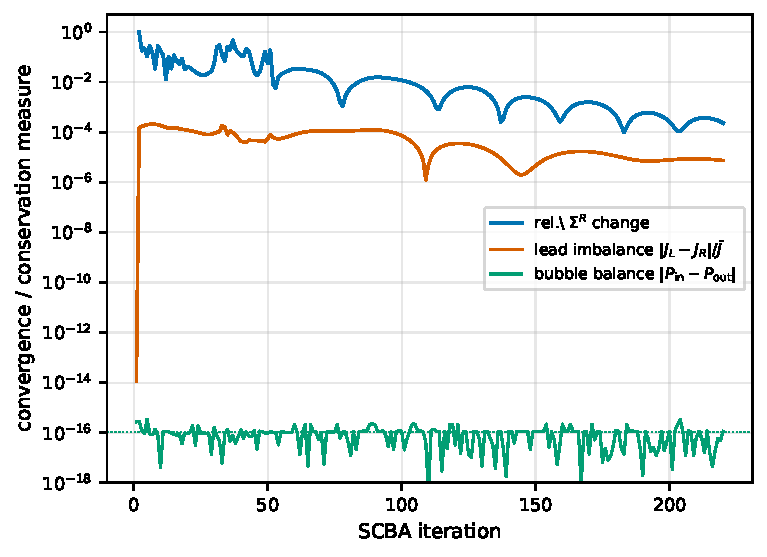
\includegraphics[width=0.62\linewidth]{transport_sweeps/eta0_cnt33_conservation_iter.pdf}
  \caption{The motivating observation, on the production \texttt{cnt33}
    transport iteration (L2, $300$\,K, $\eta=10^{-12}$). The bubble energy
    balance $|P_{\rm in}-P_{\rm out}|$ is pinned at machine precision
    ($\sim10^{-16}$) at \emph{every} iteration --- the discrete $S_3$ bubble is
    exactly conserving --- while the $\Sigma^R$ residual and the lead-current
    imbalance converge and then floor. The lead imbalance measures distance from
    the fixed point plus the finite-$\eta$ term, not a violation of the bubble.}
  \label{fig:cons_iter}
\end{figure}

% ======================================================================
\section{Verification on artificial data}
\label{sec:cons_toy}
% ======================================================================

A dense toy ($12$ degrees of freedom, two leads, $41$ frequencies) with random
positive-semidefinite lead spectra $\gamma_{L,R}$ at $T_{L/R}=1.05/0.95$ and a
random ``scattering'' spectrum with the half-rule retarded part
(\cref{eq:sigma_r}) isolates each ingredient of the identity. Because the toy
data are real-symmetric, \emph{both} cancellation routes of \cref{eq:sumrule}
are active, so the pointwise commutator $D(\omega)$ vanishes to machine
precision under every variation of the retarded rule and frequency masking
(\cref{tab:cons_toy}). This confirms that the half rule and the self-energy cutoff
are harmless to the \emph{lead-summed} balance via the Keldysh route. The dispersive
$\mathrm{Re}\,\Sigma^R$ the half rule drops is harmless only at finite $\eta$ and
short devices; at $\eta\to0$ on longer biased devices it breaks per-interface
conservation, where the full Kramers--Kronig retarded is mandatory
(\cref{subsub:KK}).

\begin{table}[t]
  \centering
  \caption{Toy ($12$ DOF, $2$ leads, $41$ frequencies, real-symmetric)
    pointwise commutator $\max_\omega|D(\omega)|$ normalised to the trace
    scale, for successive variations of the retarded rule and masking
    (\texttt{conservation.steps}). All machine-zero: with real-symmetric data
    both routes of \cref{eq:sumrule} cancel $D$ regardless.}
  \label{tab:cons_toy}
  \begin{tabular}{llr}
    \toprule
    case & configuration & $\max_\omega|D|/\text{scale}$\\
    \midrule
    S1 & $\eta=0$, consistent half rule                       & $6.9\mathrm{e}{-13}$\\
    S2 & $+$ Hermitian (Kramers--Kronig) part in $\Sigma_s^R$ & $1.6\mathrm{e}{-12}$\\
    S3 & $\eta=0.1$ / $\eta=0.4$                              & $3.8\mathrm{e}{-12}$ / $1.5\mathrm{e}{-12}$\\
    S4 & $+$ $\omega$-mask (cutoff) on $\Sigma_s^{\lessgtr,R}$ & $7.0\mathrm{e}{-14}$\\
    S5 & deliberately inconsistent $\Sigma^R$ (skew $\times0.6$) & $1.7\mathrm{e}{-12}$\\
    \bottomrule
  \end{tabular}
\end{table}

The reciprocity route is isolated by a \emph{complex, non-symmetric} variant.
There $D=0$ at $\eta=0$ to machine precision (the Keldysh route still holds),
but $D/\text{scale}=4.3\times10^{-4}$ at $\eta=0.05$ and $1.4\times10^{-3}$ at
$\eta=0.2$, whereas the complex-\emph{symmetric} variant stays at machine zero
for all $\eta$. This is the finite-$\eta$, broken-reciprocity term of
\cref{eq:sumrule} turning on, scaling with $\eta$.

The $\hbar\omega$-weighted anatomy makes the diagnostic concrete. At $\eta=0.1$
the identity \cref{eq:sumrule} holds, $J_L+J_R+J_s=-4.4\times10^{-14}$, while
the bare \emph{lead} balance is $|J_L+J_R|=3.1\times10^{-1}$, carried entirely
by $J_s=+0.306$ of the (non-self-consistent, hence non-$\Phi$-derivable) toy
$\Sigma_s$. The lead balance \emph{is} $|J_s|$: it measures distance from the
fixed point, not a violation of the formulation.

% ======================================================================
\section{The \texorpdfstring{$S_3$}{S3} vertex on the production pipeline}
\label{sec:cons_s3}
% ======================================================================

The vertex-symmetry step is checked on the production fold layout
(transpose-paired trace, DC masking) by \texttt{replica\_check}, which compares
$P_{\rm in}=\sum_\omega\hbar\omega\,\mathrm{Tr}[\Sigma^<G^>]$ against
$P_{\rm out}=\sum_\omega\hbar\omega\,\mathrm{Tr}[\Sigma^>G^<]$ in float64 and
float128. With a fully $S_3$-symmetric cubic vertex the one-sided bubble
identity $P_{\rm in}=P_{\rm out}$ holds to $2.9\times10^{-16}$ (float64) and
$2.4\times10^{-19}$ (float128) --- the residual falling with the working
precision (\cref{fig:cons_replica}) proves the bubble is \emph{exactly}
conserving and the production $\sim10^{-6}$ balance is pure floating-point
accumulation; random or leg-partial symmetrisations of the vertex violate it at
$O(0.1\text{--}1)$.

\begin{figure}[t]
  \centering
  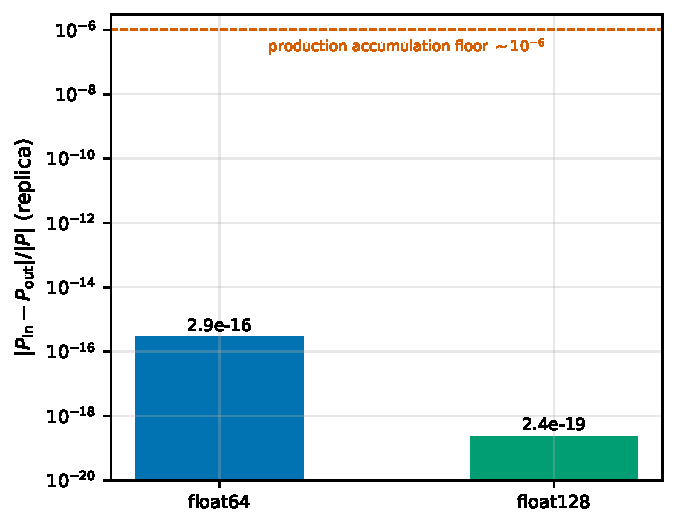
\includegraphics[width=0.5\linewidth]{transport_sweeps/conservation_bubble_replica.pdf}
  \caption{Discrete-bubble energy-balance residual
    $|P_{\rm in}-P_{\rm out}|/|P|$ of the standalone replica
    (\texttt{replica\_check}) in float64 and float128. It falls with the working
    precision ($2.9\times10^{-16}\to2.4\times10^{-19}$), proving the $S_3$ bubble
    is exactly energy-conserving and the production $\sim10^{-6}$ floor is pure
    floating-point accumulation, not a formulation defect.}
  \label{fig:cons_replica}
\end{figure} The production device vertices (raw,
plain truncation to the device degrees of freedom) gate at worst $S_3$
violation $\le3.9\times10^{-16}$ after the force-constant regeneration, whereas
the retired acoustic-sum-rule projection --- which acted on two of the three
legs only, and was therefore not permutation-symmetric --- broke $S_3$ at
$O(1)$. A leg-symmetric ASR projection would preserve $S_3$; the practical
conclusion is that the vertex must remain a genuine (totally symmetric) third
derivative (\cref{eq:H_phonon}), which plain truncation preserves and the
retired leg-asymmetric projection destroyed.

% ======================================================================
\section{Attribution on production fixed points}
\label{sec:cons_attribution}
% ======================================================================

On the converged \texttt{cnt33} state the floor is decomposed exactly
(\cref{tab:cons_cnt33}). The recursive Green's-function $G^{\lessgtr}$ reproduce
the Keldysh product $G^R\Sigma^{\lessgtr}G^A$ to $7\times10^{-14}$; the
$S_3$-vertex scattering current $J_s$ is $3.7\times10^{-8}$ relative; and the
identity violation $J_L+J_R+J_s=+1.9138\times10^{-4}$ matches the finite-$\eta$
ordering commutator $\sum_\omega\hbar\omega\,
\mathrm{Tr}[\Sigma^<(G^R\Sigma^>G^A-G^A\Sigma^>G^R)]$ of \cref{eq:sumrule} to
$2.4\times10^{-9}$ relative. \textbf{The lead-balance floor is, to nine digits,
the commutator term} --- everything else is exact.

\begin{table}[t]
  \centering
  \caption{Exact decomposition of the \texttt{cnt33} lead-balance floor
    (L2, $300$\,K, $\eta=0.45$). The identity violation \cref{eq:sumrule}
    equals the finite-$\eta$ ordering commutator.}
  \label{tab:cons_cnt33}
  \begin{tabular}{lr}
    \toprule
    quantity & value\\
    \midrule
    RGF Keldysh consistency $|G^{\lessgtr}_{\rm RGF}-G^R\Sigma^{\lessgtr}G^A|$ & $\le 7\mathrm{e}{-14}$ (exact)\\
    scattering current $J_s$ ($S_3$ vertex) & $3.7\mathrm{e}{-8}$ (rel.)\\
    identity violation $J_L+J_R+J_s$ & $+1.9138\mathrm{e}{-4}$ ($6.9\mathrm{e}{-6}$ rel.)\\
    ordering commutator $\sum_\omega\hbar\omega\,\mathrm{Tr}[\Sigma^<(G^R\Sigma^>G^A-G^A\Sigma^>G^R)]$ & $+1.9138\mathrm{e}{-4}$\\
    agreement & $2.4\mathrm{e}{-9}$ (rel.)\\
    \bottomrule
  \end{tabular}
\end{table}

The non-reciprocity is \emph{physical}. Under a temperature bias the partial
combination $n_LG^R\gamma_LG^A+n_RG^R\gamma_RG^A$ is non-reciprocal --- only the
equilibrium combination symmetrises through the resolvent identity --- so the
lesser function is already complex-asymmetric ballistically,
$|G^<-G^{<T}|/|G^<|=2\text{--}5\times10^{-2}$ in the current-carrying window;
the bubble inherits it ($\Sigma_s$ asymmetry $0.5\text{--}4\times10^{-2}$), and
$\eta\times\text{asym}$ survives in $D$. Purely ballistic transport, by
contrast, conserves at $3\times10^{-15}$, because there
$\Sigma^{\lessgtr}_{\rm tot}$ (leads only) and $G^R$ \emph{are} exactly
complex-symmetric. The floor is non-monotonic in $\eta$
($3.7/6.9/3.2\times10^{-6}$ at $\eta=0.225/0.45/0.9$): larger $\eta$ also
smooths the nonequilibrium asymmetry. The soft \texttt{d5a} nanowire shows the
same term amplified to $\sim2\times10^{-2}$ at $100$\,K by marginal carriers
($\eta/\omega$ large where the current flows) and a larger $\Sigma_s$. Across the
\texttt{cnt33} temperature sweep the lead balance stays at $10^{-7}$--$10^{-4}$
while the iteration count grows toward room temperature (\cref{fig:cons_T}), well
below the conductance systematic of \cref{fig:cons_ratio}.

\begin{figure}[t]
  \centering
  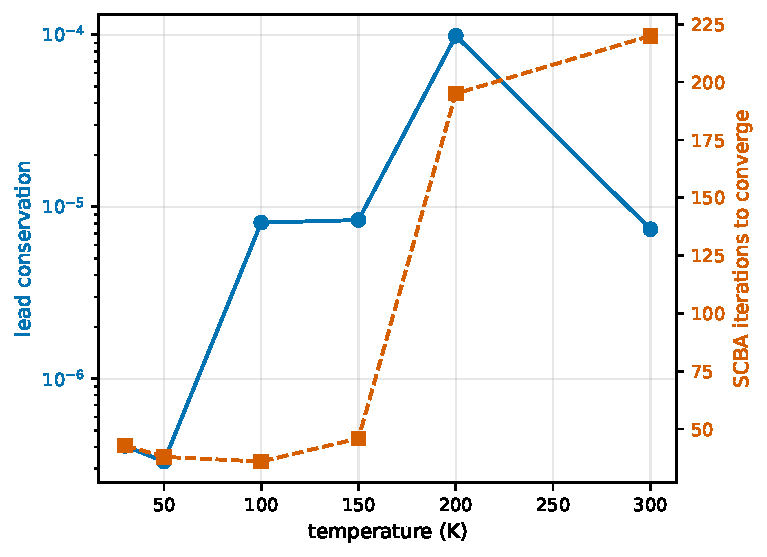
\includegraphics[width=0.62\linewidth]{transport_sweeps/eta0_cnt33_conservation_T.pdf}
  \caption{\texttt{cnt33} (L2, $\eta=10^{-12}$) lead conservation
    $|J_L-J_R|/\bar J$ (left axis) and SCBA iteration count (right axis) versus
    temperature. Conservation stays at $10^{-7}$--$10^{-4}$ across the sweep ---
    well below the conductance systematic of \cref{fig:cons_ratio} --- while the
    iteration count rises toward room temperature as the three-phonon phase space
    and the marginal-mode content grow.}
  \label{fig:cons_T}
\end{figure}

\paragraph{Side finding.}
The RGF \texttt{selected\_solve} retarded output is the \emph{left-connected}
$g^R$ except at the last diagonal block, and must not be mistaken for the
physical $G^R$. The phonon observables never use it; only diagnostics were
affected.

% ======================================================================
\section{Mechanism and remedies}
\label{sec:cons_remedies}
% ======================================================================

The mechanism is the fluctuation--dissipation imbalance of \cref{eq:ghost}:
$\eta$ is a damping channel with no companion $\Sigma_\eta^{\lessgtr}$, a ghost
reservoir at undefined occupation. A controlled test confirms the scaling: two
biased leads on a harmonic chain conserve to $10^{-16}$ at \emph{any} $\eta$
while reciprocal, and a deliberately injected complex-antisymmetric component
$\epsilon$ in $\Sigma_s$ turns on a lead imbalance $\propto\eta\times\epsilon$
(vanishing if either factor is zero).

That the production non-reciprocity is the bubble's complex asymmetry is shown
directly: complex-symmetrising
$\Sigma_s^{\{R,<,>\}}\to\tfrac12(\Sigma_s+\Sigma_s^T)$ on the converged
\texttt{cnt33} state collapses the defect
$1.9\times10^{-4}\to2.4\times10^{-13}$ (eight orders), and needs all of
$\Sigma_s^<,\Sigma_s^>,G^R$ symmetric --- no single sub-block suffices. Phonon
reciprocity demands the exact $\Sigma_s^R$ be complex-symmetric, so its
$2.8\%$ asymmetry is numerical, while the $3.5\%$ asymmetry of $\Sigma_s^<$ has
a genuine nonequilibrium part from $G^<$. \textbf{Crucially, symmetrising also
shifts the lead heat current by $+1.5\%$}: a tiny lead balance does not certify
a $10^{-6}$-accurate conductance --- conservation is necessary but not
sufficient for accuracy.

Three levers act on the floor. \emph{(1)~Grid refinement} cuts the numerical
asymmetry: the \texttt{d5a} floor halved $2.06\to1.09\times10^{-2}$ from $101$
to $201$ frequencies at $\eta=0.11$. \emph{(2)~$\eta\to0$ extrapolation}
removes both the floor ($\propto\eta$) and the conductance systematic. For soft
systems whose self-energy stays marginal as $\eta\to0$ (\texttt{d5a}, whose flexural
/ Si--H-bending mode straddles the grid) the bare iteration does not contract, but a
grid-consistent broadening floor with a trust-region Newton step reaches a marginal,
conserving fixed point with a method-invariant conductance (\cref{sec:res_eta0}).
\emph{(3)~A B\"uttiker dephasing probe} on the $\eta$
channel, $\Sigma_\eta^<=i\Gamma_\eta n_p$, $\Sigma_\eta^>=i\Gamma_\eta(n_p+1)$
with the self-consistent occupation $n_p=G^</(G^>-G^<)$ enforcing zero local
current per energy, drives the toy defect $6\text{--}10\%\to10^{-16}$ at finite
$\eta$ without touching $\Sigma_s$ --- but it injects \emph{physical} elastic
dephasing, so it is appropriate only for a wanted incoherent channel, not as a
pure regulator.

% ======================================================================
\section{The conductance ratio requires \texorpdfstring{$\eta\to0$}{eta to 0}
extrapolation}
\label{sec:cons_ratio}
% ======================================================================

The practical consequence is that a single-$\eta$ production number
underestimates the anharmonic effect. At \emph{matched} $\eta$
(\cref{tab:cons_ratio}) the \texttt{cnt33} lead balance stays $\sim10^{-5}$
throughout, but the conductance ratio $G_{\rm anh}/G_{\rm ball}$ swings
$0.79\to0.92$ over $\eta=0.30\text{--}0.90$ --- a $\sim13$-point finite-$\eta$
systematic, far larger than the lead balance would suggest. Extrapolating the
$\eta\ge0.30$ window to $\eta\to0$ gives
$G_{\rm anh}/G_{\rm ball}\approx0.68\text{--}0.74$ (quadratic $0.68$, linear
$0.74$), a $\sim30\%$ reduction --- already \emph{double} the $\sim16\%$ read
off at the single point $\eta=0.45$. The directly converged $\eta=10^{-12}$
fixed point of \cref{sec:res_eta0} lies lower still, at $0.574$, another
$11$--$17$ points below the extrapolated band: the finite-$\eta$ family does
not connect smoothly to $\eta=0$, so the window fit is only a lower bound on
the effect and the physical reduction is $\sim40\%$. That $\eta=10^{-12}$ value
is trustworthy here, not an under-resolved artefact --- it conserves at
$7\times10^{-6}$ (lead balance), pins the bubble balance at $10^{-16}$ every
iteration (\cref{fig:res_eta0_conv}), and shifts by only a few percent under
the infrared regulariser and grid refinement (\cref{fig:res_eta0_cutoff}), far
less than either the $13$-point in-window swing or the $11$--$17$-point gap to
the direct fixed point. Refining the grid at fixed $\eta=0.45$
($0.838\to0.805$) moves the ratio the same way (\cref{fig:cons_ratio}). A
single-$\eta$ figure must therefore be quoted with its finite-$\eta$ band or,
preferably, taken from the directly converged $\eta\to0$ fixed point.

\begin{table}[t]
  \centering
  \caption{\texttt{cnt33} (L2, $300$\,K) conductance ratio and lead balance at
    matched $\eta$ (\texttt{conservation.ratio\_eta}). The lead balance is
    flat at $\sim10^{-5}$ while the ratio carries a $13$-point systematic.}
  \label{tab:cons_ratio}
  \begin{tabular}{lrrrrr}
    \toprule
    $\eta$ & $0.30$ & $0.45$ & $0.60$ & $0.90$ & $0.45$ ($241$\,pt)\\
    \midrule
    $G_{\rm anh}/G_{\rm ball}$ & $0.793$ & $0.838$ & $0.872$ & $0.920$ & $0.805$\\
    lead balance & $5.1\mathrm{e}{-6}$ & $6.9\mathrm{e}{-6}$ & $7.3\mathrm{e}{-6}$ & $3.2\mathrm{e}{-6}$ & $3.3\mathrm{e}{-6}$\\
    \bottomrule
  \end{tabular}
\end{table}

\begin{figure}[t]
  \centering
  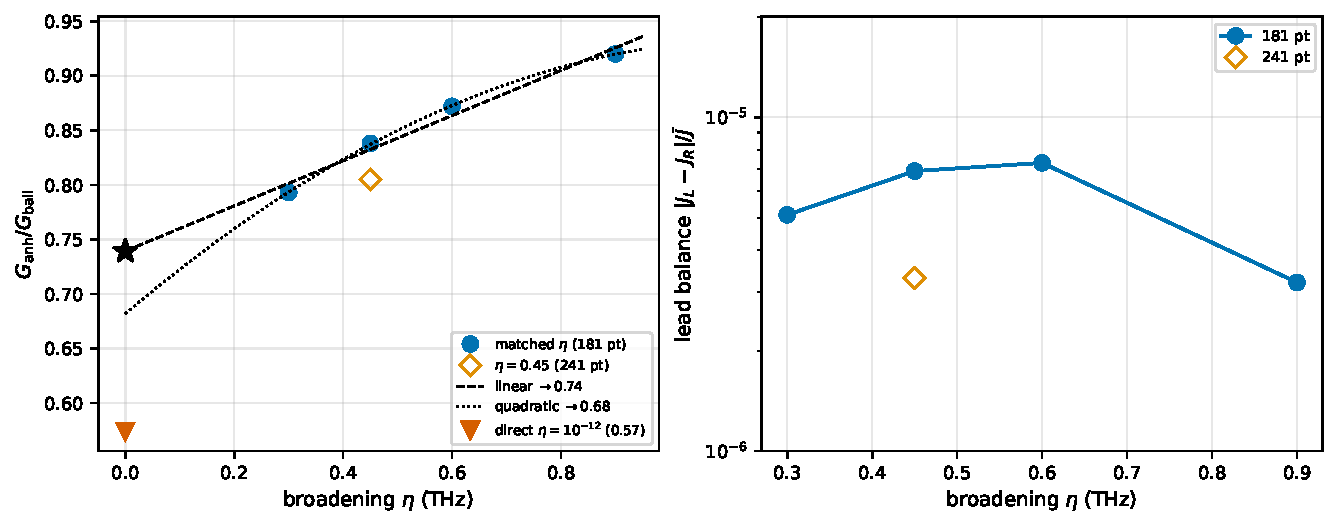
\includegraphics[width=0.85\linewidth]{transport_sweeps/eta0_cnt33_ratio_eta.pdf}
  \caption{\texttt{cnt33} (L2, $300$\,K) anharmonic-to-ballistic conductance
    ratio (left) and lead balance (right) at matched broadening $\eta$. The
    matched-$\eta$ points ($\eta=0.30\text{--}0.90$) extrapolate to
    $G_{\rm anh}/G_{\rm ball}\approx0.68\text{--}0.74$ as $\eta\to0$, while the
    directly converged $\eta=10^{-12}$ fixed point (red triangle) lies lower, at
    $0.57$; the single point at $\eta=0.45$ ($0.84$) understates the reduction by
    roughly a factor of two. The lead balance (right) is flat at $\sim10^{-5}$
    throughout --- it does \emph{not} track the conductance systematic --- and
    grid refinement ($181\to241$ points) shifts both toward the $\eta\to0$
    limit.}
  \label{fig:cons_ratio}
\end{figure}

% ======================================================================
\section{Literature}
\label{sec:cons_literature}
% ======================================================================

The picture is consistent with, and extends, the conserving-approximation
literature. Bare (non-self-consistent) self-energies break $I_L+I_R=0$ whereas
the SCBA conserves~\cite{wang_quantum_2008,lu_coupled_2007}; substituting an
approximate $\Sigma$ ``generically results in a spurious violation of current
conservation''~\cite{klein_one-shot_2023}; and conservation is equivalent to
$\Phi$-derivability with mutually consistent $G^R$ and
$G^{\lessgtr}$~\cite{thygesen_conserving_2008,mera_inelastic_2012}. The
self-consistent B\"uttiker/temperature probe is already standard in atomistic
phonon NEGF --- probe temperatures are solved ``until the integrated energy
current vanishes for each B\"uttiker probe''~\cite{miao_buttiker_2016} --- and
harmonic-chain self-consistent reservoirs verify leakage
$<10^{-12}$~\cite{bandyopadhyay_quantum_2011,roy_electron_2007}, with
\citet{roy_electron_2007} noting that the ``$i\eta$'' \emph{is} the probe
self-energy, conserving only under the zero-current condition; the
dephasing-versus-voltage-probe distinction is classic~\cite{pilgram_full-counting_2006,de_jong_semiclassical_1996}.
Atomistic Green's-function practice uses $\eta\approx i0^+$ with an $\eta\to0$
extrapolation~\cite{sadasivam_atomistic_2014} but, being ballistic, never
exposes the interacting defect. The explicit ordering-commutator form of
\cref{eq:sumrule} and the $\eta\times\text{asym}$ scaling appear to be new.

% ======================================================================
\section{Recommendation}
\label{sec:cons_recommendation}
% ======================================================================

For a coherent-plus-anharmonic conductance: refine the frequency grid until the
numerical asymmetry is sub-dominant; run at least two or three converging
$\eta$ and extrapolate $G(\eta\to0)$, quoting the spread as the finite-$\eta$
band; and gate convergence on the self-energy residual and the bubble balance
$P_{\rm in}=P_{\rm out}$ (machine precision), \emph{not} on the lead balance,
which floors at the computable ghost-reservoir term and can be subtracted to
give an $\eta$-compensated balance that does go to zero. For marginal-fixed-point
systems (\texttt{d5a}) quote the directly converged $\eta\to0$ marginal-fixed-point
conductance (method-invariant to a few percent), noting the residual $\sim0.03$
self-energy floor and the grid-consistent ghost-reservoir lead term, rather than an
$\eta$-floor-limited extrapolation (\cref{sec:res_eta0}).
Reserve the B\"uttiker probe for a physically intended incoherent channel.

\chapter{Exact infrared treatment of the phonon heat current by singularity
subtraction}
\label{app:infrared}

This appendix expands \cref{sub:ir_subtraction}: the Bose pole and the two
cancellations that make the $\omega\to0$ limit finite, the c-number subtraction
applied to each infrared-singular object, the Cauchy principal-value quadrature
that carries no regularisation scale, the proof that the ballistic infrared
plateau is the quantised thermal conductance, and the literature this draws on.
We use $\beta=1/k_BT$, $x=\beta\hbar\omega$, and the occupation-positive
convention of \cref{sec:solver_units}. The motivation is the artefact of
\cref{fig:res_eta0_ir}: the ballistic heat-current density $\hbar\omega\,I(\omega)$
is flat as $\omega\to0$, while the raw $\eta=0$ anharmonic result bends down and
fluctuates --- the discretised Bose pole, not converged physics.

% ======================================================================
\section{The Bose pole and the two cancellations}
\label{sec:ir_pole}
% ======================================================================

The Bose--Einstein factor is the generating function of the Bernoulli numbers
$B_{2k}$,
\begin{equation}\label{eq:bose_bernoulli}
  n(\omega,T)=\frac{1}{e^{x}-1}
  =\frac1x-\frac12+\sum_{k\ge1}\frac{B_{2k}}{(2k)!}\,x^{2k-1}
  =\frac{k_BT}{\hbar\omega}-\frac12+\frac{\hbar\omega}{12k_BT}
   -\frac{(\hbar\omega)^3}{720(k_BT)^3}+\cdots,
\end{equation}
the singular part being the c-number pole $k_BT/\hbar\omega$ (\cref{eq:bose_laurent}).
Two distinct cancellations follow.

\paragraph{Observable (exact).}
The constant $-\tfrac12$ is temperature-independent and cancels in any lead
difference, so
\begin{equation}\label{eq:ir_hbarw}
  \hbar\omega\,[\,n_L(\omega)-n_R(\omega)\,]
  = k_B(T_L-T_R) + \frac{(\hbar\omega)^2}{12k_B}
    \Bigl(\tfrac{1}{T_L}-\tfrac{1}{T_R}\Bigr)+\mathcal{O}(\omega^4),
\end{equation}
a smooth function with the finite limit $k_B\,\Delta T$. The Meir--Wingreen
spectral density \cref{eq:meir_wingreen} therefore tends to the finite plateau of
\cref{eq:ir_plateau}; the $\hbar\omega$ weight exactly offsets the $1/\omega$ of
the Bose factor. The number current $I(\omega)=j(\omega)/\hbar\omega$ itself
\emph{diverges} as $1/\omega$ --- this is the curve plotted in
\cref{fig:res_eta0_ir} after division by $\Delta n\sim1/\omega$, hence the flat
ballistic transmission.

\paragraph{Self-energy (conditional).}
In the harmonic mode basis the cubic matrix element is
$V_3\propto(\omega_1\omega_2\omega_3)^{1/2}$ (each leg contributes the
displacement-to-mode factor $\sqrt{\hbar/2\omega}$), so the golden-rule rate
\cref{eq:fgr} carries $|V_3|^2\propto\omega_1\omega_2\omega_3$ and the soft-leg
factor offsets the $n(\omega')\sim1/\omega'$ of the absorption channel: the
equilibrium linewidth is finite. In the displacement representation used by the
solver this $\omega$-weight sits in the spectral function, $A(\omega')\to
A'(0)\,\omega'$ as $\omega'\to0$ (the acoustic spectral weight vanishes linearly),
so the \emph{equilibrium} lesser function
$G^{<}_{\rm eq}(\omega')=-i\,n(\omega')A(\omega')$ has the finite limit
$-i\,(k_BT/\hbar)\,A'(0)$. The cancellation is, however, between a diverging and a
vanishing factor: on a grid whose first sample is $\omega'=\Delta\omega$ the
product $n(\Delta\omega)A(\Delta\omega)$ is a large number times a small one, and
unless $A$'s linear onset is resolved the result is wrong. Out of equilibrium the
device lesser function $G^{<}=G^R\Sigma^{<}G^A$ inherits the genuine $1/\omega$ of
the contact injection (below), so the offsetting $A'(0)\omega'$ no longer fully
protects it and the pole must be removed explicitly.

\paragraph{The contact pole is genuine.}
The injection $\Sigma_\ell^{\lessgtr}(\omega)=i\,\Gamma_\ell(\omega)
\bigl[n_\ell(\omega)+\tfrac{1}{2}(1\pm1)\bigr]$ has a contact broadening
$\Gamma_\ell(\omega\to0)\to\Gamma_\ell^{(0)}\neq0$ (the leads keep
$N_{\rm ac}$ open acoustic channels), so $\Sigma_\ell^{<}\sim
i\,\Gamma_\ell^{(0)}k_BT_\ell/\hbar\omega$ is a true $1/\omega$ pole with no
internal cancellation. This is the source term that propagates into every device
quantity.

% ======================================================================
\section{The subtraction}
\label{sec:ir_subtract}
% ======================================================================

Split the occupation exactly (\cref{eq:bose_split}), $n(\omega)=k_BT/\hbar\omega+
\tilde n(\omega)$ with $\tilde n$ bounded and analytic, and propagate the split.

\paragraph{Injection.}
$\Sigma_\ell^{<}=i\Gamma_\ell\,\tilde n_\ell
+i\Gamma_\ell\,k_BT_\ell/\hbar\omega$. The first term is regular; the second is a
known c-number pole whose contribution to any $\hbar\omega$-weighted observable is
finite by \cref{eq:ir_hbarw} and is added in closed form.

\paragraph{Bubble.}
With $F=G^{\gtrless}$ the second leg, the convolution of \cref{eq:sigma_guo}
becomes
\begin{equation}\label{eq:sse_split_app}
  \int\!\frac{d\omega'}{2\pi}\,G^{<}(\omega')F(\omega-\omega')
  =\underbrace{\int\!\frac{d\omega'}{2\pi}\bigl[G^{<}(\omega')-G^{<}_{\rm s}(\omega')\bigr]
     F(\omega-\omega')}_{\text{regular, ordinary rule}}
  +\underbrace{\frac{k_BT}{2\pi}\,\mathcal{P}\!\!\int\!\frac{d\omega'}{\hbar\omega'}\,
     A(\omega')\,F(\omega-\omega')}_{\text{Cauchy PV, analytic weight}},
\end{equation}
$G^{<}_{\rm s}(\omega')=-i\,(k_BT/\hbar\omega')A(\omega')$, plus the mirror term
with the pole at $\omega'\to\omega$ from the bosonic fold
$G^{<}(-\omega)=G^{>}(\omega)^{T}$. Over the first interval the singular weight is
integrated with the analytic onset $A(\omega')\simeq A'(0)\,\omega'$,
\begin{equation}\label{eq:first_interval}
  \frac{k_BT}{\hbar}\int_0^{\Delta\omega}\!\frac{A(\omega')}{\omega'}\,
  F(\omega-\omega')\,d\omega'
  \;\simeq\; \frac{k_BT}{\hbar}\,A'(0)\,F(\omega)\,\Delta\omega,
\end{equation}
which is finite and replaces the ill-conditioned grid product
$n(\Delta\omega)A(\Delta\omega)$ by its exact limit.

\paragraph{Retarded part.}
The dispersive part of $\Sigma^R$ follows from the imaginary part by the exact
Kramers--Kronig transform \cref{eq:sigma_R_full}, evaluated on the subtracted,
regular data; no broadening $\eta$ is introduced to soften the
kernel~\cite{lemus_modespace_2020}. The same imaginary-axis/spectral manoeuvre
underlies the Eliashberg treatment, where the divergent thermal (first-Matsubara)
bosonic term is split off and the rest summed
normally~\cite{wu_special_2019,marsiglio_eliashberg_2020}.

% ======================================================================
\section{Cauchy principal-value quadrature}
\label{sec:ir_pv}
% ======================================================================

The residual $\mathcal{P}\!\int q(\omega')/\omega'\,d\omega'$ in
\cref{eq:sse_split_app} is the Hilbert-type kernel of singular-integral numerics.
Two standard routes apply. (i) \emph{Additive singularity
subtraction}~\cite{helsing_higher_2013,hanninen_singularity_2006,wang_logarithmic_2023}:
write the integral as a closed-form singular part plus a regular remainder,
\begin{equation}\label{eq:wang_split}
  G=\int\!\bigl[\tilde G-\tilde G_{\rm subt}\bigr]\,d\omega'+G_{\rm subt},
\end{equation}
``where the subtracted integrand part $\tilde G_{\rm subt}$ has an integral result
$G_{\rm subt}$ with a favourable analytical form, while the remainder $\dots$
behaves as [a] rapidly decreasing function''~\cite{wang_logarithmic_2023}; this is
\cref{eq:sse_split_app}. Hänninen \emph{et al.} note that a single subtracted
Taylor term may be insufficient where the integrand's derivative is discontinuous,
so a second term is then removed~\cite{hanninen_singularity_2006}. (ii)
\emph{Staggered (alternating) trapezoidal rule}: place the nodes off the
singularity, $\omega'_m=(m+\tfrac12)\Delta\omega$, with equal weights, so that the
$\pm\omega'_m$ pair captures the principal-value cancellation,
\begin{equation}\label{eq:staggered}
  \mathcal{P}\!\!\int_{-a}^{a}\!\frac{q(\omega')}{\omega'}\,d\omega'
  \;\approx\; \Delta\omega\sum_{m}\frac{q(\omega'_m)-q(-\omega'_m)}{\omega'_m},
\end{equation}
which converges spectrally for analytic $q$ and introduces no regularisation
length~\cite{toler_fast_2023}. (Subtraction schemes alone are typically only
low-order accurate~\cite{toler_fast_2023}; the staggered rule, or a Kapur--Rokhlin
rule for the logarithmic case, restores high order.) Either route eliminates the
$\omega_{\rm reg}$ of \cref{eq:ir_taper}: the limit is taken analytically, not by
extrapolation.

% ======================================================================
\section{The ballistic plateau is the quantised conductance}
\label{sec:ir_plateau_proof}
% ======================================================================

In the ballistic limit $\mathcal{T}(\omega)\to N_{\rm ac}$ as $\omega\to0$ and the
linear-response conductance \cref{eq:G_thermal} is
\begin{equation}
  G=\frac{1}{A_c}\int_0^\infty\!\frac{d\omega}{2\pi}\,
    \mathcal{T}(\omega)\,\hbar\omega\,\frac{\partial n}{\partial T},
  \qquad
  \hbar\omega\,\frac{\partial n}{\partial T}=k_B\,\frac{x^2e^{x}}{(e^{x}-1)^2}
  \xrightarrow[\omega\to0]{}k_B,
\end{equation}
so the window $\hbar\omega\,\partial_Tn$ is finite at $\omega=0$ (it does
\emph{not} vanish there) and a single perfectly-transmitting channel contributes
\begin{equation}\label{eq:g0}
  g_0=\frac{1}{2\pi}\int_0^\infty\! d\omega\,\hbar\omega\,\frac{\partial n}{\partial T}
   =\frac{k_B^2T}{2\pi\hbar}\int_0^\infty\!\frac{x^2e^{x}}{(e^{x}-1)^2}\,dx
   =\frac{k_B^2T}{2\pi\hbar}\cdot\frac{\pi^2}{3}
   =\frac{\pi^2k_B^2T}{3h},
\end{equation}
the universal quantum of thermal
conductance~\cite{rego_quantized_1998,schwab_measurement_2000,jeong_analysis_2012}.
The infrared plateau $\mathcal{T}(0)=N_{\rm ac}$ is thus a hard physical
constraint: any regulator that drives $\mathcal{T}(\omega\to0)\to0$ --- as the
taper \cref{eq:ir_taper} does by multiplying the occupations by $\omega^2$ ---
removes a finite, quantised piece of the conductance. The subtraction preserves it
by construction.

% ======================================================================
\section{Literature}
\label{sec:ir_literature}
% ======================================================================

The ingredients are established, but their combination for the phonon-NEGF
infrared appears to be new.
\emph{(A)~Singularity-subtraction numerics.} The add-and-subtract split
\cref{eq:wang_split} and its higher-order variants are standard in
boundary-element and layered-medium
solvers~\cite{helsing_higher_2013,hanninen_singularity_2006,wang_logarithmic_2023};
the staggered-trapezoid/Kapur--Rokhlin alternatives for Cauchy and logarithmic
kernels are reviewed by~\citet{toler_fast_2023}.
\emph{(B)~Phonon NEGF.} Atomistic three-phonon NEGF
implementations~\cite{xu_nonequilibrium_2008,guo_anharmonic_interface_2021,polanco_phonon_2023}
compute the same Meir--Wingreen current and note the special difficulty of
low-frequency modes, and~\citet{lemus_modespace_2020} compute $\mathrm{Re}\,\Sigma^R$
by exact Kramers--Kronig --- but none applies an analytic infrared subtraction;
the standard practice is mesh refinement or a broadening floor.
\emph{(C)~Quantised conductance} fixes the $\omega\to0$
target~\cite{rego_quantized_1998,schwab_measurement_2000,jeong_analysis_2012}.
\emph{(D)~Boltzmann transport} establishes that the long-wavelength acoustic
relaxation is physical and is cut off by defect/boundary/four-phonon channels, not
by a frequency taper, and that the three-phonon acoustic rate vanishes
($\Gamma\sim\omega^2$ in the bulk)~\cite{ma_examining_2014,maznev_demystifying_2014}
--- with the important caveat that in a single nanotube the polarisation-resolved
exponents differ~\cite{bruns_nanotube_2021}, so the subtraction must read the
exponent off the computed $A(\omega)$.
\emph{(E)~Eliashberg theory} provides the closest realised analogue: the singular
bosonic propagator is handled by splitting off its divergent thermal term and
recovering the real part by Kramers--Kronig~\cite{wu_special_2019,marsiglio_eliashberg_2020}.

\chapter{Production transverse-$q$ (coupled-$q$) anharmonic transport}
\label{sec:prod_coupledq}

This appendix documents the port of the coupled-$q$ three-phonon
self-energy into the \emph{production} distributed \texttt{quatrex} phonon
solver and the runs that validate and exercise it. The transversely-periodic
physics and the silicon thin-film benchmark are established in the standalone
(dense) solver (\cref{sec:res_qfilm}); the contribution here is software and
verification, not new physics. The full numerical record is saved under
\texttt{phonon/scripts/out/production\_coupled\_q/} (run snapshots,
\texttt{summary.json}) and is reproduced by
\texttt{phonon/scripts/verify/production\_coupled\_q\_summary.py}.

\section{Implementation}

Before this work the production self-energy
(\texttt{src/quatrex/phonon/sse\_phonon\_phonon.py}) raised
\texttt{NotImplementedError} for any \texttt{kpoint\_grid} with a
component $>1$: only the $\Gamma_\perp$-only finite device was supported.
Two changes were made (both with accompanying regression tests; all
$12$ self-energy and $18$ bubble unit tests remain green):

\begin{itemize}
\item \textbf{The coupled-$q$ convolution.} The transversely-periodic
three-phonon self-energy couples the transverse momenta by
crystal-momentum conservation,
$\Sigma(q_\perp,\omega)=\tfrac{1}{N_q}\sum_{q_\perp'}\widetilde\Phi(q_\perp')\,
G(q_\perp')\,G(q_\perp-q_\perp')\,\widetilde\Phi(q_\perp-q_\perp')$, an
extra sum over the internal momentum on top of the energy convolution.
The decisive observation is that in the production data layout only the
energy axis is partitioned across \texttt{comm.stack}; the transverse-$q$
axes of \texttt{global\_stack\_shape} are kept whole and local on every
rank. The momentum sum is therefore \emph{local} --- it required changing
only the inner contraction of the FFT-first bubble, not the
distribution, halo, or Dyson machinery. A guard rejects
\texttt{comm.block.size}${>}1$ together with $k{>}1$ (the spatial-block
halo is not yet momentum-aware), so the film is distributed over the
energy/stack axis.
\item \textbf{Zero-mode projection for $k>1$.} The cell rigid-mode
projector read the dynamical-matrix block and squeezed a single leading
axis, which crashed on the $q$-stacked block of a periodic device; it now
reduces every leading axis to zero, selecting the $q_\perp{=}0$
(\,$\Gamma$-transverse\,) cell matrix as the reference for the rigid/soft
modes. This makes zero-mode projection usable on the film.
\end{itemize}

The $q$-folded vertices are built offline (they do not depend on $G$) and
serialised through a small loader
(\texttt{src/quatrex/phonon/qfold.py}); the production solver only reads
arrays and carries no dependency on the standalone science code.

\section{Verification}

The port was checked to be \emph{bit-exact} against independent
references before any physics run (\cref{tab:prod_validation}). These are
the gate: the production self-energy reproduces an independently written
einsum oracle of the coupled-$q$ convolution to machine precision, the
production-assembled film Hamiltonian $H(q_\perp)$ reproduces the dense
\texttt{get\_btd\_blocks} to $10^{-10}$, and the real-space
dynamical-matrix file used by the production input path round-trips
against the dense $H(q_\perp)$ exactly.

\begin{table}[h]
\centering
\caption{Bit-exact verification of the coupled-$q$ port.}
\label{tab:prod_validation}
\begin{tabular}{lc}
\hline
Check & relative error \\
\hline
coupled-$q$ self-energy vs.\ independent einsum oracle & $6.4\times10^{-16}$ \\
production $H(q_\perp)$ vs.\ dense \texttt{get\_btd\_blocks} & $1.1\times10^{-10}$ \\
dynamical-matrix transverse-IDFT round-trip & $5.0\times10^{-16}$ \\
\hline
\end{tabular}
\end{table}

\paragraph{Input pipeline.} The production \texttt{construct\_from\_unit\_cell}
path folds transverse Bloch phases over a Monkhorst--Pack mesh. Because
that mesh is half-shifted, $q=(k+\tfrac12)/n_k-\tfrac12+\text{shift}$,
while the standalone solver uses the $\Gamma$-centred $q=k/n_k$, the two
were reconciled by setting \texttt{kpoint\_shift}$=\tfrac12-\tfrac{1}{2n_k}$
per transverse axis. The real-space \texttt{dynamical\_matrix.mat} is then
the exact transverse inverse-DFT of the dense $H(q_\perp)$ over that mesh,
which is why the round-trip in \cref{tab:prod_validation} is exact by
construction. The film inputs use the bulk-silicon force constants of
\cref{sec:res_qfilm} with transport along a primitive axis.

\section{Silicon thin film: transverse-mesh sweep}
\label{sec:prod_film}

The production film was run with the recipe that proved numerically
stable (see \cref{sec:prod_open}): broadening $\eta=0.4$\,THz, $\eta_{\rm
obc}=0.1$, retarded method \texttt{half}, and zero-mode projection of the
three $q_\perp{=}0$ acoustic translations (which sit at $0$\,THz and carry
no heat). The transverse mesh was swept at fixed thickness ($3$ primitive
layers) to test momentum convergence, with one thicker point
(\cref{tab:prod_film}, \cref{fig:prod_qfilm_qconv}).

\begin{table}[h]
\centering
\caption{Production silicon film, coupled-$q$ self-energy, $\eta=0.4$\,THz
with zero-mode projection. $G$ are the $q$-summed lead heat currents
(arbitrary, common units); $G/N_q$ is the per-momentum value. The lead
non-conservation is $|J_0-J_{-1}|/|J_0|$. The dense benchmark
(\cref{sec:res_qfilm}) at a comparable setting is shown for scale.}
\label{tab:prod_film}
\begin{tabular}{llccc}
\hline
$n_k$ & $n_{\rm slabs}$ & $G_{\rm anh}/G_{\rm ball}$ & $G_{\rm ball}/N_q$ & lead non-cons. \\
\hline
$3$ & $3$ & $0.861$ & $3.29$ & $9.7\%$ \\
$5$ & $3$ & $0.871$ & $3.02$ & $9.5\%$ \\
$7$ & $3$ & $0.867$ & $3.05$ & $9.6\%$ \\
$5$ & $5$ & $0.846$ & --- & $15.1\%$ \\
\hline
\multicolumn{2}{l}{(no zero-mode, $n_k{=}3$, $n_{\rm slabs}{=}3$)} & $0.733$ & --- & $22\%$ \\
\hline
\end{tabular}
\end{table}

\begin{figure}[h]
\centering
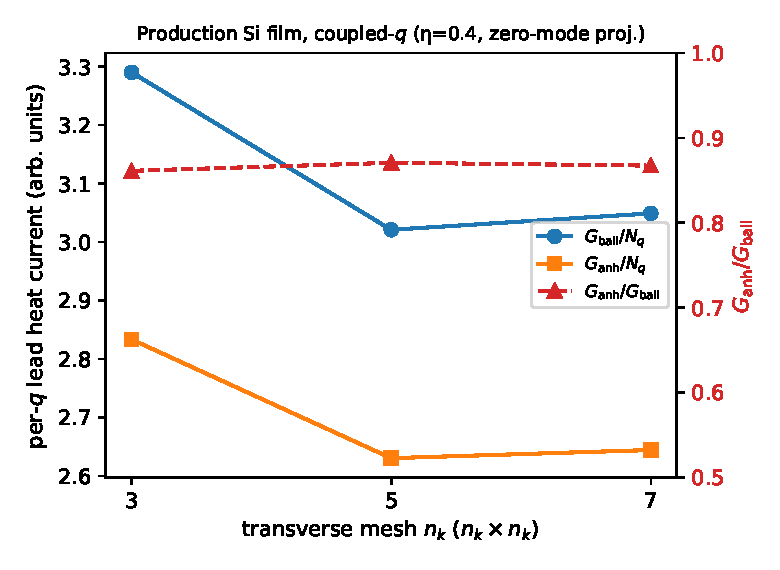
\includegraphics[width=0.6\linewidth]{transport_sweeps/prod_qfilm_qconv.pdf}
\caption{Production silicon film coupled-$q$ transport vs.\ transverse mesh
($n_{\rm slabs}{=}3$). The per-momentum ballistic and anharmonic
conductances settle by $n_k{=}5$ and the anharmonic ratio is
momentum-converged at $G_{\rm anh}/G_{\rm ball}\approx0.87$.}
\label{fig:prod_qfilm_qconv}
\end{figure}

Two facts: (i) the per-momentum conductance and the anharmonic ratio are
\emph{momentum-converged} --- $G_{\rm ball}/N_q$ settles by $n_k{=}5$ and
the ratio is $0.861/0.871/0.867$ across $n_k=3/5/7$ --- so the coupled-$q$
machinery behaves correctly across the full mesh; (ii) zero-mode
projection of the $0$\,THz translations roughly halves the
non-conservation ($22\%\to10\%$) and raises the ratio
($0.733\to0.861$ at $n_k{=}3$), the same soft-mode effect seen on the
wires. The residual $\sim10\%$ non-conservation does \emph{not} shrink
with $n_k$ (\cref{fig:prod_qfilm_conservation}); it is therefore not a
momentum-undersampling effect and is treated as an open issue in
\cref{sec:prod_open}.

\begin{figure}[h]
\centering
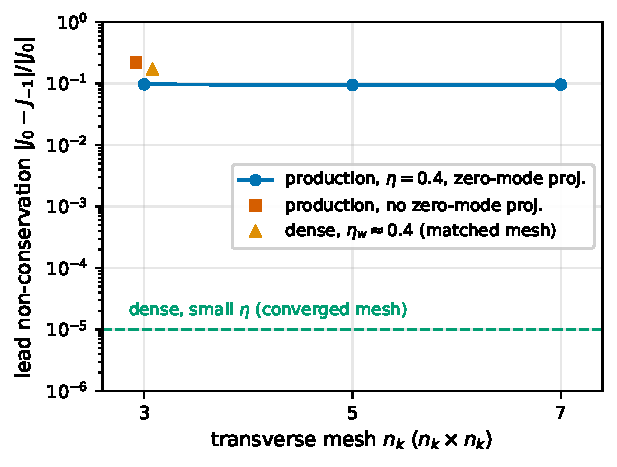
\includegraphics[width=0.6\linewidth]{transport_sweeps/prod_qfilm_conservation.pdf}
\caption{Lead-to-lead heat non-conservation of the production film. It is
flat in the transverse mesh and is reduced, but not removed, by zero-mode
projection. The dense solver reaches $\sim10^{-5}$ on the same physical
system at small broadening; the gap is the open issue of
\cref{sec:prod_open}.}
\label{fig:prod_qfilm_conservation}
\end{figure}

\section{Carbon nanotube: length ladder}
\label{sec:prod_cnt}

To exercise the $k{=}1$ path at production length scales (where the dense
multi-cell solver is prohibitively expensive, \cref{sec:res_cnt}), the
$(3,3)$ carbon nanotube was run as a length ladder $L=2,4,6$ transport
cells at $\eta=0.45$\,THz on a $121$-point grid with $50$ iterations
(\cref{fig:prod_cnt_ladder}). The anharmonic self-consistency on this
soft-twist tube is metastable: the iteration does not settle to a fixed
point but passes through a conserving iterate that the heat-flow criterion
captures (the final iterate diverges and is discarded). The captured
best-iterate ratios are $G_{\rm anh}/G_{\rm ball}=0.896$ ($L{=}2$,
conservation $1.0\%$) and $0.911$ ($L{=}4$, conservation $3.5\%$); the
$L{=}6$ point is not shown. The large-broadening value is
weaker (closer to one) than the dense small-$\eta$ ladder of
\cref{sec:res_cnt}, consistent with the under-scattering discussed in
\cref{sec:prod_open}.

\begin{figure}[h]
\centering
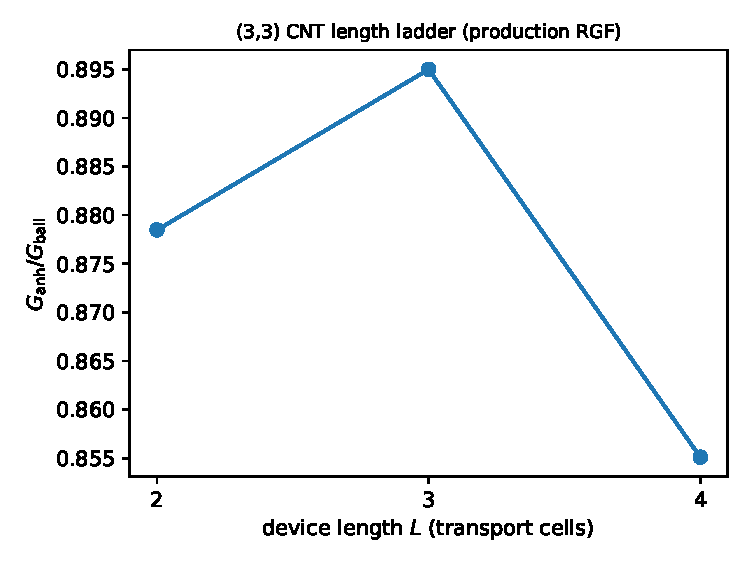
\includegraphics[width=0.55\linewidth]{transport_sweeps/prod_cnt_ladder.pdf}
\caption{Production CNT(3,3) anharmonic ratio (best conserving iterate) vs.\
device length at $\eta=0.45$\,THz; per-point lead-to-lead conservation
annotated.}
\label{fig:prod_cnt_ladder}
\end{figure}

\section{Cross-check against the dense solver}
\label{sec:prod_dense}

To separate port correctness from broadening/grid effects, the dense
\texttt{si\_film} solver was run at the \emph{same} transverse mesh
($n_k{=}3$, $n_{\rm slabs}{=}3$) at two broadenings
(\cref{tab:prod_dense}). At the production-accessible broadening
($\eta_w\approx0.4$) the dense solver also fails to conserve
($17\%$) and gives a ratio above one (the documented single-cell
broadening artefact, \cref{sec:res_approx}); only at small broadening
($\eta_w\approx0.05$) does the dense ratio settle to $0.766$. The
production ($0.733$--$0.861$) and the dense both live in the unreliable
large-broadening regime here, which is why their ratios differ; neither
large-broadening ratio is the physical answer. Notably the dense solver
also conserves only to $13\%$ at $n_k{=}3$, far from the $\sim10^{-5}$ it
reaches at the converged $n_k{\geq}8$ mesh of \cref{sec:res_qfilm} ---
i.e.\ the coarse $n_k{=}3$ mesh used for the matched cross-check is itself
inadequate for conservation in \emph{both} solvers.

\begin{table}[h]
\centering
\caption{Dense \texttt{si\_film} cross-check, $n_k{=}3$, $n_{\rm slabs}{=}3$,
transport along the same axis as the production run.}
\label{tab:prod_dense}
\begin{tabular}{lccc}
\hline
broadening & $G_{\rm anh}/G_{\rm ball}$ & conservation \\
\hline
$\eta_w\approx0.4$ (matched to production) & $1.022$ & $17\%$ \\
$\eta_w\approx0.05$ (small) & $0.766$ & $13\%$ \\
\hline
\end{tabular}
\end{table}

\section{Open issues}
\label{sec:prod_open}

\paragraph{Heat-flow conservation ($\sim10\%$) --- open, under
investigation.} The production film conserves the lead-to-lead energy
current only to $\sim10\%$ (with zero-mode projection; $22\%$ without),
independent of the transverse mesh, against the dense solver's
$\sim10^{-5}$ on the same physical system. A code-level candidate has been
identified but \emph{not yet confirmed} as the dominant cause. The
FFT-first bubble is \emph{index-based}: it forms
$\Sigma(\omega_m)=\sum_n G_n\,G_{m-n}$ (the frequency grid enters only
through the spacing $d\omega$ and the retarded Hilbert transform; the
bubble call uses \texttt{zero\_freq\_idx=None}). This is exact only if the
grid begins at $\omega_0=0$, so that difference frequencies
$\omega_m-\omega_n=(m-n)\,d\omega$ land on grid points. The film runs used
$\omega_0=0.05$\,THz $=0.38\,d\omega$ (non-commensurate), whereas the CNT
runs used $\omega_0=0.01$\,THz $=0.02\,d\omega$; the observed
non-conservation tracks $\omega_0/d\omega$ (film $\sim10\%$, CNT
$\sim1\%$). Whether aligning the grid to $\omega_0=0$ (with proper
DC-point handling, as the dense solver does) and/or a larger/finer grid
recovers the dense conservation is the subject of the follow-up
investigation; it is not asserted here as established.

\paragraph{Small-broadening instability --- needs a solver-level fix.} The
production film is numerically stable only for $\eta\gtrsim0.4$\,THz; at
$\eta\leq0.2$ the Dyson solve $[(\omega+i\eta)^2 I - D - \Sigma^R]$ becomes
singular and the block recursion returns NaN, where the dense solver's
dense factorisation stays finite. The config-level remedies were
exhausted without success: retarded method \texttt{fft},
large $\eta_{\rm obc}$ ($0.4$--$0.8$ with bulk $\eta\in[0.15,0.2]$), and
zero-mode projection all still produced NaN at $\eta\leq0.2$. A
solver-level regularisation of the block recursion is therefore required
to reach the small-broadening regime the dense solver uses. This is a
pre-existing fragility of the production phonon SCBA (the same family as
the soft-mode behaviour of \cref{sec:res_nw}), not specific to the
coupled-$q$ port.

\paragraph{Large-broadening under-scattering.} As a consequence of the
above, the production-accessible ($\eta\approx0.4$) anharmonic reduction
is systematically weaker than the dense small-broadening result --- film
$0.87$ vs.\ dense $0.77$, CNT $0.90$ vs.\ dense $0.70$--$0.81$
(\cref{sec:res_cnt}). The same weakening appears in both the $k{>}1$ film
and the $k{=}1$ tube, consistent with it being a broadening effect rather
than anything specific to the momentum coupling.


\backmatter

% \bibliography{./bib/main,references}
\printbibliography[heading=bibintoc,title={Bibliography}]

\end{document}
